\documentclass{book}
\usepackage[a4paper,top=2.5cm,bottom=2.5cm,left=2.5cm,right=2.5cm]{geometry}
\usepackage{makeidx}
\usepackage{natbib}
\usepackage{graphicx}
\usepackage{multicol}
\usepackage{float}
\usepackage{listings}
\usepackage{color}
\usepackage{ifthen}
\usepackage[table]{xcolor}
\usepackage{textcomp}
\usepackage{alltt}
\usepackage{ifpdf}
\ifpdf
\usepackage[pdftex,
            pagebackref=true,
            colorlinks=true,
            linkcolor=blue,
            unicode
           ]{hyperref}
\else
\usepackage[ps2pdf,
            pagebackref=true,
            colorlinks=true,
            linkcolor=blue,
            unicode
           ]{hyperref}
\usepackage{pspicture}
\fi
\usepackage[utf8]{inputenc}
\usepackage{mathptmx}
\usepackage[scaled=.90]{helvet}
\usepackage{courier}
\usepackage{sectsty}
\usepackage{amssymb}
\usepackage[titles]{tocloft}
\usepackage{doxygen}
\lstset{language=C++,inputencoding=utf8,basicstyle=\footnotesize,breaklines=true,breakatwhitespace=true,tabsize=4,numbers=left }
\makeindex
\setcounter{tocdepth}{3}
\renewcommand{\footrulewidth}{0.4pt}
\renewcommand{\familydefault}{\sfdefault}
\hfuzz=15pt
\setlength{\emergencystretch}{15pt}
\hbadness=750
\tolerance=750
\begin{document}
\hypersetup{pageanchor=false,citecolor=blue}
\begin{titlepage}
\vspace*{7cm}
\begin{center}
{\Large Ba\-Ka\-Plan \\[1ex]\large 0.\-7 }\\
\vspace*{1cm}
{\large Generated by Doxygen 1.8.3.1}\\
\vspace*{0.5cm}
{\small Sun May 19 2013 20:32:43}\\
\end{center}
\end{titlepage}
\clearemptydoublepage
\pagenumbering{roman}
\tableofcontents
\clearemptydoublepage
\pagenumbering{arabic}
\hypersetup{pageanchor=true,citecolor=blue}
\chapter{Main Page}
\label{index}\hypertarget{index}{}This software creates seating plan for examinations. It provides five different strategies to create seat plan.

\subsection*{R\-E\-Q\-U\-I\-R\-E\-M\-E\-N\-T\-S\-: }

\begin{DoxyVerb}1) GNU G++ Compiler
2) Configure public_html and cgi-bin in home
3) CGICC Library
4) MySQL Connector for C++
5) Boost Library
6) jwSMTP Library
7) libharu PDF Library
8) exim4 mail server
\end{DoxyVerb}


Installation of requirements

1) G\-N\-U G++ Compiler

Run following command in terminal to install \begin{DoxyVerb}$ sudo apt-get install g++
\end{DoxyVerb}


2) Configure public\-\_\-html/cgi-\/bin folder for executing files on browser.\par
 Assuming you already installed apache if not then run following command in terminal \begin{DoxyVerb}$ sudo apt-get install apache2
\end{DoxyVerb}


{\bfseries Steps to configure public\-\_\-html} \begin{DoxyVerb}$ mkdir ~/public_html

$ sudo a2enmod userdir

$ sudo service apache2 restart
\end{DoxyVerb}


Give 755 permissions to public\-\_\-html directory \begin{DoxyVerb}$ chmod -R 755 ~/public_html
\end{DoxyVerb}


Now open \href{http://localhost/~username}{\tt http\-://localhost/$\sim$username} in browser. Here username is your login name.

{\bfseries Steps to configure cgi-\/bin in public\-\_\-html} \begin{DoxyVerb}$ sudo a2enmod cgi

$ sudo a2enmod cgid

$ sudo service apache2 restart

$ cd ~/public_html

$ mkdir cgi-bin

$ cd /etc/apache2

$ sudo vim sites-available/default
\end{DoxyVerb}


Add following text in file\-: \begin{DoxyVerb}ScriptAlias /cgi-bin/ /home/*/public_html/cgi-bin/
<Directory "/home/*/public_html/cgi-bin">
    AllowOverride None
    Options +ExecCGI -MultiViews +SymLinksIfOwnerMatch
    SetHandler cgi-script
    Order allow,deny
    Allow from all
</Directory>
\end{DoxyVerb}


Save it and then restart apache \begin{DoxyVerb}$ sudo service apache2 restart
\end{DoxyVerb}


3) C\-G\-I\-C\-C Library\par


Run following command in terminal \begin{DoxyVerb}$ sudo apt-get install libcgicc-dev
\end{DoxyVerb}


O\-R

Download any latest package from \href{http://ftp.gnu.org/gnu/cgicc/}{\tt http\-://ftp.\-gnu.\-org/gnu/cgicc/}\par


Then run following commands in terminal \begin{DoxyVerb}$ tar xzf cgicc-X.X.X.tar.gz 

$ cd cgicc-X.X.X/ 

$ ./configure --prefix=/usr 

$ make

$ sudo make install
\end{DoxyVerb}


4) My\-S\-Q\-L and My\-S\-Q\-L Connector for C++

Run following commands in terminal \begin{DoxyVerb}$ sudo apt-get install mysql-server mysql-client

$ sudo apt-get install libmysql++

$ sudo apt-get install libmysql++-dev
\end{DoxyVerb}


5) Boost Library

Run following command in terminal \begin{DoxyVerb}$ sudo apt-get install libboost1.53-dev 
\end{DoxyVerb}


6) jw\-S\-M\-T\-P Library

Download \href{http://sourceforge.net/projects/jwsmtp/files/latest/download}{\tt jw\-S\-M\-T\-P} Library

Follow steps to install \begin{DoxyVerb}$ cd ~/Downloads
$ tar -xzf jwsmtp-X.X.X.tar.gz
$ cd jwsmtp-X.X.X
$ ./configure
$ make
$ sudo make install

NOTE: If you got error in */mailer.cpp or */demo2.cpp file then
include string header file in that. And again run make
\end{DoxyVerb}


7) libharu P\-D\-F Library

Download \href{https://github.com/libharu/libharu/tarball/master}{\tt libharu} Library

Follow the steps to install \begin{DoxyVerb}$ cd ~/Downloads
$ tar -xzf libharu-libharu-RELEASE_2_3_0RC2-61-g22e741e.tar.gz
$ cd libharu-libharu-22e741e
$ cmake -G 'Unix Makefiles'
$ make
$ sudo make install

NOTE: If you get any error regarding cmake, then run
$ sudo apt-get install cmake
to install cmake
\end{DoxyVerb}


8) exim4 Mail Server

Run the following commands in terminal \begin{DoxyVerb}$ sudo apt-get install exim4
$ sudo dpkg-reconfigure exim4-config
\end{DoxyVerb}


A Mail Server Configuration window will appear.\par
 Follow the following instructions to configure the mail server. \begin{DoxyVerb}1) The first page is just and introduction. Press ENTER
2) On the second page choose the second option i.e 
   mail sent by smarthost; received via SMTP or fetchmail and 
   press ENTER.
3) Next Keep the system mail name as it is and press ENTER.
4) Just Press Enter for the next page.
5) The next page asks you to enter IP addresses to listen on
   incoming SMTP connections. Leave it as it is and Press ENTER
6) Even on the next page let the value be the default one and 
   Press ENTER.
7) Leave the next page as it is and Press ENTER.
8) The next page asks you for IP address or host name of the outgoing
   smarthost. Enter “smtp.example.com::587″. Where example refers to
   gmail, yahoo or any other mail service provider and 587 is port number.
9) The Next page asks you if you want to hide local mail name in 
   outgoing mail? Choose “No”.
10)The Next asks you if you want to keep number of DNS-queries minimal?
   Choose “No”.
11)On the next page choose the  delivery method for local mail as
   mbox format in /var/mail/.
12)Next page asks you if you want to split configuration into small
   files? Choose “No”. 
13)Next keep root and postmaster mail recipient empty.
\end{DoxyVerb}


Now terminal will show that M\-T\-A is being restarted.\par
 After this is done, run the following command in terminal \begin{DoxyVerb}$ sudo vim /etc/exim4/passwd.client
\end{DoxyVerb}


Add following in the file \begin{DoxyVerb}*:USERNAME@example.com:PASSWORD.

Where, USERNAME is  a valid email address and PASSWORD is  password for USERNAME.
\end{DoxyVerb}


\subsection*{I\-N\-S\-T\-A\-L\-L\-A\-T\-I\-O\-N\-: }

Check \href{https://github.com/GreatDevelopers/bakaplan/blob/master/INSTALLATION.txt}{\tt I\-N\-S\-T\-A\-L\-L\-A\-T\-I\-O\-N} steps for using this software.

\subsection*{A\-U\-T\-H\-O\-R\-S\-: }

{\bfseries Mentor and Manager}

Dr. Hardeep Singh Rai

Website\-: \href{http://gndec.ac.in/~hsrai}{\tt http\-://gndec.\-ac.\-in/$\sim$hsrai}

{\bfseries \href{https://github.com/GreatDevelopers/bakaplan/wiki/Contributors}{\tt Developers}}

\href{https://github.com/megha55}{\tt Mandeep Kaur}

Website\-: \href{http://simak.in}{\tt http\-://simak.\-in}

\href{https://github.com/Jaskaran28193}{\tt Jaskaran Singh Lamba}

Blog\-: \href{http://lambajaskaran.wordpress.com/}{\tt http\-://lambajaskaran.\-wordpress.\-com/}

Email\-: baithnekaplan \mbox{[}A\-T\mbox{]} gmail.\-com 
\chapter{Hierarchical Index}
\section{\-Class \-Hierarchy}
\-This inheritance list is sorted roughly, but not completely, alphabetically\-:\begin{DoxyCompactList}
\item \contentsline{section}{\-Database}{\pageref{de/d03/classDatabase}}{}
\item \contentsline{section}{\-Data\-Sheet}{\pageref{dd/dcc/classDataSheet}}{}
\item \contentsline{section}{\-Exapand\-Roll\-No}{\pageref{d2/d9b/classExapandRollNo}}{}
\item \contentsline{section}{\-Input\-Detail}{\pageref{db/d6e/classInputDetail}}{}
\begin{DoxyCompactList}
\item \contentsline{section}{\-Class\-Detail}{\pageref{d9/ddf/classClassDetail}}{}
\item \contentsline{section}{\-Date\-Sheet}{\pageref{de/d0e/classDateSheet}}{}
\item \contentsline{section}{\-Exam\-Detail}{\pageref{df/d4d/classExamDetail}}{}
\begin{DoxyCompactList}
\item \contentsline{section}{\-Valid\-Strategy}{\pageref{d9/d15/classValidStrategy}}{}
\end{DoxyCompactList}
\item \contentsline{section}{\-Login}{\pageref{dd/dfd/classLogin}}{}
\begin{DoxyCompactList}
\item \contentsline{section}{\-Project\-Detail}{\pageref{d3/dd8/classProjectDetail}}{}
\end{DoxyCompactList}
\item \contentsline{section}{\-Report}{\pageref{da/da8/classReport}}{}
\item \contentsline{section}{\-Roll\-No\-Detail}{\pageref{d6/db0/classRollNoDetail}}{}
\item \contentsline{section}{\-Room\-Detail}{\pageref{d4/de5/classRoomDetail}}{}
\item \contentsline{section}{\-Strategy}{\pageref{d2/df2/classStrategy}}{}
\end{DoxyCompactList}
\item \contentsline{section}{\-Input\-Field\-Name}{\pageref{dd/db2/classInputFieldName}}{}
\item \contentsline{section}{\-Java\-Script}{\pageref{da/dac/classJavaScript}}{}
\item \contentsline{section}{\-Page\-Structure\-Maker}{\pageref{de/d88/classPageStructureMaker}}{}
\begin{DoxyCompactList}
\item \contentsline{section}{\-Page\-Layout}{\pageref{d7/d9e/classPageLayout}}{}
\end{DoxyCompactList}
\item \contentsline{section}{\-Read\-Input}{\pageref{de/d50/classReadInput}}{}
\begin{DoxyCompactList}
\item \contentsline{section}{\-Arrange\-Roll\-No}{\pageref{da/de9/classArrangeRollNo}}{}
\begin{DoxyCompactList}
\item \contentsline{section}{\-Date\-Sheet}{\pageref{de/d0e/classDateSheet}}{}
\end{DoxyCompactList}
\item \contentsline{section}{\-Expand\-Roll\-No}{\pageref{d0/d6e/classExpandRollNo}}{}
\item \contentsline{section}{\-Seat\-Plan}{\pageref{d2/d41/classSeatPlan}}{}
\begin{DoxyCompactList}
\item \contentsline{section}{\-Strategy}{\pageref{d2/df2/classStrategy}}{}
\end{DoxyCompactList}
\end{DoxyCompactList}
\item \contentsline{section}{\-Read\-Input\-Field}{\pageref{d8/d37/classReadInputField}}{}
\item \contentsline{section}{\-Send\-Mail}{\pageref{d6/d66/classSendMail}}{}
\end{DoxyCompactList}

\chapter{Class Index}
\section{Class List}
Here are the classes, structs, unions and interfaces with brief descriptions\-:\begin{DoxyCompactList}
\item\contentsline{section}{\hyperlink{classArrangeRollNo}{Arrange\-Roll\-No} }{\pageref{classArrangeRollNo}}{}
\item\contentsline{section}{\hyperlink{classBranchDetails}{Branch\-Details} }{\pageref{classBranchDetails}}{}
\item\contentsline{section}{\hyperlink{classBranchReport}{Branch\-Report} }{\pageref{classBranchReport}}{}
\item\contentsline{section}{\hyperlink{classExamDetails}{Exam\-Details} }{\pageref{classExamDetails}}{}
\item\contentsline{section}{\hyperlink{classExapandRollNo}{Exapand\-Roll\-No} }{\pageref{classExapandRollNo}}{}
\item\contentsline{section}{\hyperlink{classHome}{Home} }{\pageref{classHome}}{}
\item\contentsline{section}{\hyperlink{classHomeCSS}{Home\-C\-S\-S} }{\pageref{classHomeCSS}}{}
\item\contentsline{section}{\hyperlink{classHTMLTags}{H\-T\-M\-L\-Tags} \\*Base class containong Basic Html Tags and methods }{\pageref{classHTMLTags}}{}
\item\contentsline{section}{\hyperlink{classReadBranchDetails}{Read\-Branch\-Details} }{\pageref{classReadBranchDetails}}{}
\item\contentsline{section}{\hyperlink{classReadExamDetails}{Read\-Exam\-Details} }{\pageref{classReadExamDetails}}{}
\item\contentsline{section}{\hyperlink{classReadInput}{Read\-Input} }{\pageref{classReadInput}}{}
\item\contentsline{section}{\hyperlink{classReadRollNoDetails}{Read\-Roll\-No\-Details} }{\pageref{classReadRollNoDetails}}{}
\item\contentsline{section}{\hyperlink{classReadRoomDetails}{Read\-Room\-Details} }{\pageref{classReadRoomDetails}}{}
\item\contentsline{section}{\hyperlink{classReport}{Report} }{\pageref{classReport}}{}
\item\contentsline{section}{\hyperlink{classRollNoDetails}{Roll\-No\-Details} }{\pageref{classRollNoDetails}}{}
\item\contentsline{section}{\hyperlink{classRoomDetails}{Room\-Details} }{\pageref{classRoomDetails}}{}
\item\contentsline{section}{\hyperlink{classRoomReport}{Room\-Report} }{\pageref{classRoomReport}}{}
\item\contentsline{section}{\hyperlink{classSeatPlan}{Seat\-Plan} }{\pageref{classSeatPlan}}{}
\item\contentsline{section}{\hyperlink{classStrategy}{Strategy} }{\pageref{classStrategy}}{}
\item\contentsline{section}{\hyperlink{classSubjectWiseRollNo}{Subject\-Wise\-Roll\-No} }{\pageref{classSubjectWiseRollNo}}{}
\item\contentsline{section}{\hyperlink{classValidation}{Validation} }{\pageref{classValidation}}{}
\end{DoxyCompactList}

\chapter{File Index}
\section{File List}
Here is a list of all documented files with brief descriptions\-:\begin{DoxyCompactList}
\item\contentsline{section}{frontend/src/\hyperlink{adduser-main_8cpp}{adduser-\/main.\-cpp} \\*Adding new user and setting its password }{\pageref{adduser-main_8cpp}}{}
\item\contentsline{section}{frontend/src/\hyperlink{class-main_8cpp}{class-\/main.\-cpp} \\*Main method }{\pageref{class-main_8cpp}}{}
\item\contentsline{section}{frontend/src/\hyperlink{class_8cc}{class.\-cc} \\*\hyperlink{classClassDetail}{Class\-Detail} function definition }{\pageref{class_8cc}}{}
\item\contentsline{section}{frontend/src/\hyperlink{confirm-main_8cpp}{confirm-\/main.\-cpp} \\*Main method to call Confirm\-Page of \hyperlink{classLogin}{Login} class and creating confirm.\-html page }{\pageref{confirm-main_8cpp}}{}
\item\contentsline{section}{frontend/src/{\bfseries database.\-cc} }{\pageref{database_8cc}}{}
\item\contentsline{section}{frontend/src/\hyperlink{datesheet-main_8cpp}{datesheet-\/main.\-cpp} \\*Main method }{\pageref{datesheet-main_8cpp}}{}
\item\contentsline{section}{frontend/src/{\bfseries datesheet.\-cc} }{\pageref{datesheet_8cc}}{}
\item\contentsline{section}{frontend/src/\hyperlink{exam-main_8cpp}{exam-\/main.\-cpp} \\*Main method }{\pageref{exam-main_8cpp}}{}
\item\contentsline{section}{frontend/src/\hyperlink{exam_8cc}{exam.\-cc} \\*\hyperlink{classExamDetail}{Exam\-Detail} Class func. definition }{\pageref{exam_8cc}}{}
\item\contentsline{section}{frontend/src/{\bfseries inputdetail.\-cc} }{\pageref{inputdetail_8cc}}{}
\item\contentsline{section}{frontend/src/{\bfseries inputfieldname.\-cc} }{\pageref{inputfieldname_8cc}}{}
\item\contentsline{section}{frontend/src/\hyperlink{javascript_8cc}{javascript.\-cc} \\*Function definition of javascript class }{\pageref{javascript_8cc}}{}
\item\contentsline{section}{frontend/src/\hyperlink{login-main_8cpp}{login-\/main.\-cpp} \\*Main Function for create login.\-html page }{\pageref{login-main_8cpp}}{}
\item\contentsline{section}{frontend/src/{\bfseries login.\-cc} }{\pageref{login_8cc}}{}
\item\contentsline{section}{frontend/src/\hyperlink{logout-main_8cpp}{logout-\/main.\-cpp} \\*Log out user account }{\pageref{logout-main_8cpp}}{}
\item\contentsline{section}{frontend/src/{\bfseries md5.\-cc} }{\pageref{md5_8cc}}{}
\item\contentsline{section}{frontend/src/{\bfseries newuser-\/main.\-cpp} }{\pageref{newuser-main_8cpp}}{}
\item\contentsline{section}{frontend/src/{\bfseries pagelayout.\-cc} }{\pageref{pagelayout_8cc}}{}
\item\contentsline{section}{frontend/src/{\bfseries pagestructure.\-cc} }{\pageref{pagestructure_8cc}}{}
\item\contentsline{section}{frontend/src/{\bfseries project-\/main.\-cpp} }{\pageref{project-main_8cpp}}{}
\item\contentsline{section}{frontend/src/{\bfseries project.\-cc} }{\pageref{project_8cc}}{}
\item\contentsline{section}{frontend/src/{\bfseries readinputfield.\-cc} }{\pageref{readinputfield_8cc}}{}
\item\contentsline{section}{frontend/src/\hyperlink{register-main_8cpp}{register-\/main.\-cpp} \\*Main method for register.\-html }{\pageref{register-main_8cpp}}{}
\item\contentsline{section}{frontend/src/\hyperlink{report-main_8cpp}{report-\/main.\-cpp} \\*Main method }{\pageref{report-main_8cpp}}{}
\item\contentsline{section}{frontend/src/{\bfseries report.\-cc} }{\pageref{report_8cc}}{}
\item\contentsline{section}{frontend/src/{\bfseries reset-\/main.\-cpp} }{\pageref{reset-main_8cpp}}{}
\item\contentsline{section}{frontend/src/\hyperlink{rollno-main_8cpp}{rollno-\/main.\-cpp} \\*Main method }{\pageref{rollno-main_8cpp}}{}
\item\contentsline{section}{frontend/src/\hyperlink{rollno_8cc}{rollno.\-cc} \\*Roll\-No detail Class definition }{\pageref{rollno_8cc}}{}
\item\contentsline{section}{frontend/src/\hyperlink{room-main_8cpp}{room-\/main.\-cpp} \\*Main method }{\pageref{room-main_8cpp}}{}
\item\contentsline{section}{frontend/src/\hyperlink{room_8cc}{room.\-cc} \\*\hyperlink{classRoomDetail}{Room\-Detail} class definition }{\pageref{room_8cc}}{}
\item\contentsline{section}{frontend/src/\hyperlink{sendmail_8cc}{sendmail.\-cc} \\*Function Definitons of \hyperlink{classSendMail}{Send\-Mail} Class }{\pageref{sendmail_8cc}}{}
\item\contentsline{section}{frontend/src/\hyperlink{strategy-main_8cpp}{strategy-\/main.\-cpp} \\*Main method }{\pageref{strategy-main_8cpp}}{}
\item\contentsline{section}{frontend/src/{\bfseries strategy.\-cc} }{\pageref{strategy_8cc}}{}
\item\contentsline{section}{frontend/src/\hyperlink{validstrategy-main_8cpp}{validstrategy-\/main.\-cpp} \\*Main method }{\pageref{validstrategy-main_8cpp}}{}
\item\contentsline{section}{frontend/src/{\bfseries validstrategy.\-cc} }{\pageref{validstrategy_8cc}}{}
\item\contentsline{section}{frontend/src/backend/\hyperlink{arrangerollno_8cc}{arrangerollno.\-cc} \\*Function definition of \hyperlink{classArrangeRollNo}{Arrange\-Roll\-No} class }{\pageref{arrangerollno_8cc}}{}
\item\contentsline{section}{frontend/src/backend/{\bfseries datesheet.\-cc} }{\pageref{backend_2datesheet_8cc}}{}
\item\contentsline{section}{frontend/src/backend/\hyperlink{expandrollno_8cc}{expandrollno.\-cc} \\*Function definition of \hyperlink{classExpandRollNo}{Expand\-Roll\-No} class defintion }{\pageref{expandrollno_8cc}}{}
\item\contentsline{section}{frontend/src/backend/\hyperlink{main_8cpp}{main.\-cpp} \\*Main Method }{\pageref{main_8cpp}}{}
\item\contentsline{section}{frontend/src/backend/\hyperlink{readinput_8cc}{readinput.\-cc} \\*Function Definition of \hyperlink{classReadInput}{Read\-Input} Class }{\pageref{readinput_8cc}}{}
\item\contentsline{section}{frontend/src/backend/{\bfseries report.\-cc} }{\pageref{backend_2report_8cc}}{}
\item\contentsline{section}{frontend/src/backend/\hyperlink{seatplan_8cc}{seatplan.\-cc} \\*Function definition of \hyperlink{classSeatPlan}{Seat\-Plan} Class }{\pageref{seatplan_8cc}}{}
\item\contentsline{section}{frontend/src/backend/{\bfseries strategy.\-cc} }{\pageref{backend_2strategy_8cc}}{}
\item\contentsline{section}{frontend/src/backend/header/\hyperlink{arrangerollno_8h}{arrangerollno.\-h} \\*\hyperlink{classArrangeRollNo}{Arrange\-Roll\-No} class for arranging roll no, sorting, and removing roll nos that are not required for seating plan }{\pageref{arrangerollno_8h}}{}
\item\contentsline{section}{frontend/src/backend/header/{\bfseries datesheet.\-h} }{\pageref{backend_2header_2datesheet_8h}}{}
\item\contentsline{section}{frontend/src/backend/header/\hyperlink{expandrollno_8h}{expandrollno.\-h} \\*\hyperlink{classExpandRollNo}{Expand\-Roll\-No} class declaration for expanding roll nos }{\pageref{expandrollno_8h}}{}
\item\contentsline{section}{frontend/src/backend/header/{\bfseries filename.\-h} }{\pageref{backend_2header_2filename_8h}}{}
\item\contentsline{section}{frontend/src/backend/header/{\bfseries header.\-h} }{\pageref{backend_2header_2header_8h}}{}
\item\contentsline{section}{frontend/src/backend/header/\hyperlink{readinput_8h}{readinput.\-h} \\*Declaration of \hyperlink{classReadInput}{Read\-Input} class for reading input details from file }{\pageref{readinput_8h}}{}
\item\contentsline{section}{frontend/src/backend/header/{\bfseries report.\-h} }{\pageref{backend_2header_2report_8h}}{}
\item\contentsline{section}{frontend/src/backend/header/\hyperlink{seatplan_8h}{seatplan.\-h} \\*Declaration of \hyperlink{classSeatPlan}{Seat\-Plan} class for generating seating plan }{\pageref{seatplan_8h}}{}
\item\contentsline{section}{frontend/src/backend/header/{\bfseries strategy.\-h} }{\pageref{backend_2header_2strategy_8h}}{}
\item\contentsline{section}{frontend/src/header/{\bfseries cgicc.\-h} }{\pageref{cgicc_8h}}{}
\item\contentsline{section}{frontend/src/header/\hyperlink{class_8h}{class.\-h} \\*\hyperlink{classClassDetail}{Class\-Detail} Class declaration }{\pageref{class_8h}}{}
\item\contentsline{section}{frontend/src/header/{\bfseries constant.\-h} }{\pageref{constant_8h}}{}
\item\contentsline{section}{frontend/src/header/{\bfseries database-\/detail.\-h} }{\pageref{database-detail_8h}}{}
\item\contentsline{section}{frontend/src/header/{\bfseries database.\-h} }{\pageref{database_8h}}{}
\item\contentsline{section}{frontend/src/header/{\bfseries datesheet.\-h} }{\pageref{header_2datesheet_8h}}{}
\item\contentsline{section}{frontend/src/header/\hyperlink{exam_8h}{exam.\-h} \\*\hyperlink{classExamDetail}{Exam\-Detail} class for exam detail }{\pageref{exam_8h}}{}
\item\contentsline{section}{frontend/src/header/{\bfseries filename.\-h} }{\pageref{header_2filename_8h}}{}
\item\contentsline{section}{frontend/src/header/{\bfseries header.\-h} }{\pageref{header_2header_8h}}{}
\item\contentsline{section}{frontend/src/header/{\bfseries inputdetail.\-h} }{\pageref{inputdetail_8h}}{}
\item\contentsline{section}{frontend/src/header/{\bfseries inputfieldname.\-h} }{\pageref{inputfieldname_8h}}{}
\item\contentsline{section}{frontend/src/header/{\bfseries javascript.\-h} }{\pageref{javascript_8h}}{}
\item\contentsline{section}{frontend/src/header/{\bfseries login.\-h} }{\pageref{login_8h}}{}
\item\contentsline{section}{frontend/src/header/{\bfseries md5.\-h} }{\pageref{md5_8h}}{}
\item\contentsline{section}{frontend/src/header/{\bfseries pagelayout.\-h} }{\pageref{pagelayout_8h}}{}
\item\contentsline{section}{frontend/src/header/{\bfseries pagestructure.\-h} }{\pageref{pagestructure_8h}}{}
\item\contentsline{section}{frontend/src/header/{\bfseries project.\-h} }{\pageref{project_8h}}{}
\item\contentsline{section}{frontend/src/header/{\bfseries readinputfield.\-h} }{\pageref{readinputfield_8h}}{}
\item\contentsline{section}{frontend/src/header/{\bfseries report.\-h} }{\pageref{header_2report_8h}}{}
\item\contentsline{section}{frontend/src/header/\hyperlink{rollno_8h}{rollno.\-h} \\*Roll\-No class declaration for taking roll no detail }{\pageref{rollno_8h}}{}
\item\contentsline{section}{frontend/src/header/\hyperlink{room_8h}{room.\-h} \\*\hyperlink{classRoomDetail}{Room\-Detail} class }{\pageref{room_8h}}{}
\item\contentsline{section}{frontend/src/header/\hyperlink{sendmail-detail_8h}{sendmail-\/detail.\-h} \\*S\-M\-T\-P swttings detail }{\pageref{sendmail-detail_8h}}{}
\item\contentsline{section}{frontend/src/header/\hyperlink{sendmail_8h}{sendmail.\-h} \\*Declaration of \hyperlink{classSendMail}{Send\-Mail} Class usinf jw\-S\-M\-T\-P library }{\pageref{sendmail_8h}}{}
\item\contentsline{section}{frontend/src/header/{\bfseries strategy.\-h} }{\pageref{header_2strategy_8h}}{}
\item\contentsline{section}{frontend/src/header/{\bfseries validstrategy.\-h} }{\pageref{validstrategy_8h}}{}
\end{DoxyCompactList}

\chapter{Class Documentation}
\hypertarget{classArrangeRollNo}{\section{\-Arrange\-Roll\-No \-Class \-Reference}
\label{classArrangeRollNo}\index{\-Arrange\-Roll\-No@{\-Arrange\-Roll\-No}}
}


\-Arrange roll no class for sorting, removing redundant roll nos and also excludeing roll nos that are not for seating plan.  




{\ttfamily \#include $<$arrangerollno.\-h$>$}

\-Inheritance diagram for \-Arrange\-Roll\-No\-:\begin{figure}[H]
\begin{center}
\leavevmode
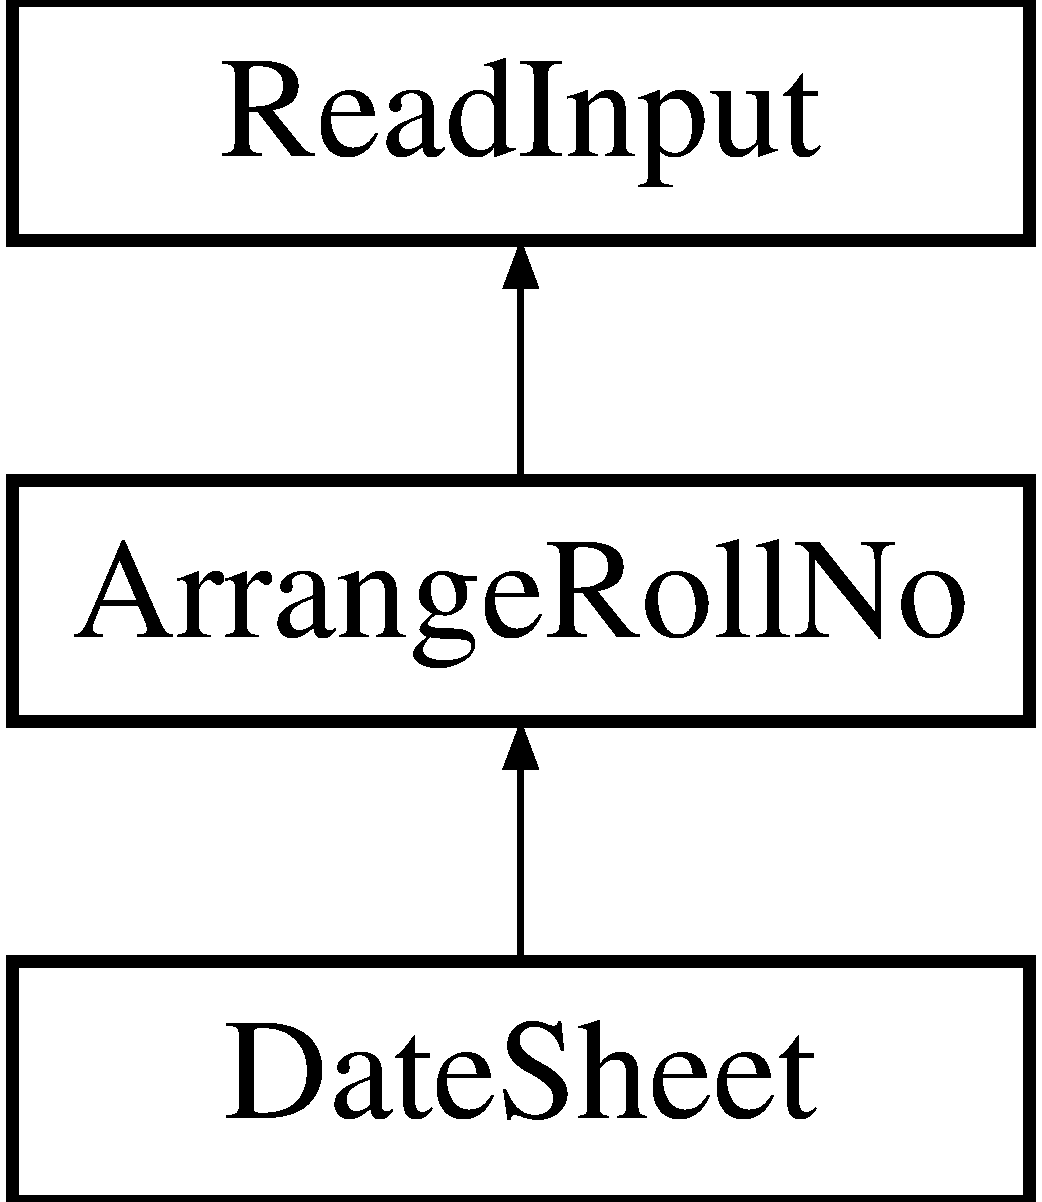
\includegraphics[height=3.000000cm]{classArrangeRollNo}
\end{center}
\end{figure}
\subsection*{\-Public \-Member \-Functions}
\begin{DoxyCompactItemize}
\item 
\hyperlink{classArrangeRollNo_a430515990d97ffa02b65ed5d15d79c9f}{\-Arrange\-Roll\-No} ()
\begin{DoxyCompactList}\small\item\em \-Constructor. \end{DoxyCompactList}\item 
void \hyperlink{classArrangeRollNo_aae9734fb7b98d980d3f1feb1b52a6195}{\-Sort\-Roll\-No} (\-I\-N\-T\-\_\-\-V\-E\-C \&rollno)
\begin{DoxyCompactList}\small\item\em \-Function for sorting roll no vector array. \end{DoxyCompactList}\item 
void \hyperlink{classArrangeRollNo_ab0b6350a9113b86925133d7199929020}{\-Remove\-Redundancy} (\-I\-N\-T\-\_\-\-V\-E\-C \&rollno)
\item 
void \hyperlink{classArrangeRollNo_adeb652c1977c668d2cd519c1a4f317bd}{\-Remove\-Non\-Eligible\-Roll\-No} (\-I\-N\-T\-\_\-\-V\-E\-C \&rollno, \-I\-N\-T\-\_\-\-V\-E\-C \&\hyperlink{classArrangeRollNo_a1f6740950e3180731b74c3ecdc19b98c}{not\-Included\-R\-No})
\begin{DoxyCompactList}\small\item\em \-Removing roll no that are not eligible. \end{DoxyCompactList}\item 
void \hyperlink{classArrangeRollNo_a69151212acbfeb90780b066ade988418}{\-Add\-Prefix\-With\-Roll\-No} (\-I\-N\-T\-\_\-\-V\-E\-C \&rollno, \-S\-T\-R\-I\-N\-G\-\_\-\-V\-E\-C \&\hyperlink{classArrangeRollNo_ac70b1f6e601cc5786ef339a38ae18c6f}{prefix})
\begin{DoxyCompactList}\small\item\em \-Adding prefix with roll nos. \end{DoxyCompactList}\item 
void \hyperlink{classArrangeRollNo_a12e17989e12519e37083b7f5649ebbec}{\-Write\-Arranged\-Roll\-No} ()
\begin{DoxyCompactList}\small\item\em \-Writing arranged roll nos to file as \-O/p file. \end{DoxyCompactList}\item 
void \hyperlink{classArrangeRollNo_a795fde3b512631e07d7189138b39b775}{\-Main} (string p\-I\-D)
\begin{DoxyCompactList}\small\item\em \-Main function to call all functions. \end{DoxyCompactList}\item 
\hyperlink{classArrangeRollNo_acbdaa06590d381ec19a7a07c718b9282}{$\sim$\-Arrange\-Roll\-No} ()
\begin{DoxyCompactList}\small\item\em \-Destructor. \end{DoxyCompactList}\end{DoxyCompactItemize}
\subsection*{\-Protected \-Attributes}
\begin{DoxyCompactItemize}
\item 
\-I\-N\-T\-\_\-\-V\-E\-C \hyperlink{classArrangeRollNo_ad75d3ee3f709606da5b4871098c3e978}{roll\-No}
\item 
\-I\-N\-T\-\_\-\-V\-E\-C \hyperlink{classArrangeRollNo_a1f6740950e3180731b74c3ecdc19b98c}{not\-Included\-R\-No}
\item 
\hypertarget{classArrangeRollNo_ab39f82c658365388d106b3dcc18e69fb}{\-I\-N\-T\-\_\-\-V\-E\-C {\bfseries roll\-No\-Size}}\label{classArrangeRollNo_ab39f82c658365388d106b3dcc18e69fb}

\item 
\hypertarget{classArrangeRollNo_a728b87c54815f5393e93da5909ed90b2}{\-I\-N\-T\-\_\-\-V\-E\-C {\bfseries not\-Included\-R\-No\-Size}}\label{classArrangeRollNo_a728b87c54815f5393e93da5909ed90b2}

\item 
\-S\-T\-R\-I\-N\-G\-\_\-\-V\-E\-C \hyperlink{classArrangeRollNo_ac70b1f6e601cc5786ef339a38ae18c6f}{prefix}
\item 
\-S\-T\-R\-I\-N\-G\-\_\-2\-D\-V\-E\-C \hyperlink{classArrangeRollNo_aa0401159b5d59c7afe77980a391a9a0a}{prefix\-Roll\-No}
\item 
\hyperlink{classExpandRollNo}{\-Expand\-Roll\-No} \hyperlink{classArrangeRollNo_a7ddd59b57f85cf6fea265d38c284df92}{expand\-R\-No}
\end{DoxyCompactItemize}


\subsection{\-Detailed \-Description}
\-Arrange roll no class for sorting, removing redundant roll nos and also excludeing roll nos that are not for seating plan. 

\-Include \hyperlink{arrangerollno_8h}{arrangerollno.\-h} file

\-Include \hyperlink{expandrollno_8h}{expandrollno.\-h} file 

\-Definition at line 30 of file arrangerollno.\-h.



\subsection{\-Constructor \& \-Destructor \-Documentation}
\hypertarget{classArrangeRollNo_a430515990d97ffa02b65ed5d15d79c9f}{\index{\-Arrange\-Roll\-No@{\-Arrange\-Roll\-No}!\-Arrange\-Roll\-No@{\-Arrange\-Roll\-No}}
\index{\-Arrange\-Roll\-No@{\-Arrange\-Roll\-No}!ArrangeRollNo@{\-Arrange\-Roll\-No}}
\subsubsection[{\-Arrange\-Roll\-No}]{\setlength{\rightskip}{0pt plus 5cm}{\bf \-Arrange\-Roll\-No\-::\-Arrange\-Roll\-No} (
\begin{DoxyParamCaption}
{}
\end{DoxyParamCaption}
)}}\label{classArrangeRollNo_a430515990d97ffa02b65ed5d15d79c9f}


\-Constructor. 

\-Constructor 

\-Definition at line 27 of file arrangerollno.\-cc.

\hypertarget{classArrangeRollNo_acbdaa06590d381ec19a7a07c718b9282}{\index{\-Arrange\-Roll\-No@{\-Arrange\-Roll\-No}!$\sim$\-Arrange\-Roll\-No@{$\sim$\-Arrange\-Roll\-No}}
\index{$\sim$\-Arrange\-Roll\-No@{$\sim$\-Arrange\-Roll\-No}!ArrangeRollNo@{\-Arrange\-Roll\-No}}
\subsubsection[{$\sim$\-Arrange\-Roll\-No}]{\setlength{\rightskip}{0pt plus 5cm}{\bf \-Arrange\-Roll\-No\-::$\sim$\-Arrange\-Roll\-No} (
\begin{DoxyParamCaption}
{}
\end{DoxyParamCaption}
)}}\label{classArrangeRollNo_acbdaa06590d381ec19a7a07c718b9282}


\-Destructor. 

\-Desrtuctor 

\-Definition at line 212 of file arrangerollno.\-cc.



\subsection{\-Member \-Function \-Documentation}
\hypertarget{classArrangeRollNo_a69151212acbfeb90780b066ade988418}{\index{\-Arrange\-Roll\-No@{\-Arrange\-Roll\-No}!\-Add\-Prefix\-With\-Roll\-No@{\-Add\-Prefix\-With\-Roll\-No}}
\index{\-Add\-Prefix\-With\-Roll\-No@{\-Add\-Prefix\-With\-Roll\-No}!ArrangeRollNo@{\-Arrange\-Roll\-No}}
\subsubsection[{\-Add\-Prefix\-With\-Roll\-No}]{\setlength{\rightskip}{0pt plus 5cm}void {\bf \-Arrange\-Roll\-No\-::\-Add\-Prefix\-With\-Roll\-No} (
\begin{DoxyParamCaption}
\item[{\-I\-N\-T\-\_\-\-V\-E\-C \&}]{roll\-No, }
\item[{\-S\-T\-R\-I\-N\-G\-\_\-\-V\-E\-C \&}]{prefix}
\end{DoxyParamCaption}
)}}\label{classArrangeRollNo_a69151212acbfeb90780b066ade988418}


\-Adding prefix with roll nos. 

\-Adding prefix with roll nos


\begin{DoxyParams}{\-Parameters}
{\em roll\-No} & \-List of eligible roll nos \\
\hline
{\em prefix} & \-Prefix ie added with roll nos \\
\hline
\end{DoxyParams}


\-Definition at line 107 of file arrangerollno.\-cc.

\hypertarget{classArrangeRollNo_a795fde3b512631e07d7189138b39b775}{\index{\-Arrange\-Roll\-No@{\-Arrange\-Roll\-No}!\-Main@{\-Main}}
\index{\-Main@{\-Main}!ArrangeRollNo@{\-Arrange\-Roll\-No}}
\subsubsection[{\-Main}]{\setlength{\rightskip}{0pt plus 5cm}void {\bf \-Arrange\-Roll\-No\-::\-Main} (
\begin{DoxyParamCaption}
\item[{string}]{p\-I\-D}
\end{DoxyParamCaption}
)}}\label{classArrangeRollNo_a795fde3b512631e07d7189138b39b775}


\-Main function to call all functions. 

\-Main method to call all function in order/sequence


\begin{DoxyParams}{\-Parameters}
{\em p\-I\-D} & \-Project \-I\-D \\
\hline
\end{DoxyParams}


\-Reimplemented in \hyperlink{classDateSheet_af749306c14297b5c93c16f48f551d5bb}{\-Date\-Sheet}.



\-Definition at line 151 of file arrangerollno.\-cc.

\hypertarget{classArrangeRollNo_adeb652c1977c668d2cd519c1a4f317bd}{\index{\-Arrange\-Roll\-No@{\-Arrange\-Roll\-No}!\-Remove\-Non\-Eligible\-Roll\-No@{\-Remove\-Non\-Eligible\-Roll\-No}}
\index{\-Remove\-Non\-Eligible\-Roll\-No@{\-Remove\-Non\-Eligible\-Roll\-No}!ArrangeRollNo@{\-Arrange\-Roll\-No}}
\subsubsection[{\-Remove\-Non\-Eligible\-Roll\-No}]{\setlength{\rightskip}{0pt plus 5cm}void {\bf \-Arrange\-Roll\-No\-::\-Remove\-Non\-Eligible\-Roll\-No} (
\begin{DoxyParamCaption}
\item[{\-I\-N\-T\-\_\-\-V\-E\-C \&}]{roll\-No, }
\item[{\-I\-N\-T\-\_\-\-V\-E\-C \&}]{not\-Included\-R\-No}
\end{DoxyParamCaption}
)}}\label{classArrangeRollNo_adeb652c1977c668d2cd519c1a4f317bd}


\-Removing roll no that are not eligible. 

\-Removing non eligible roll nos


\begin{DoxyParams}{\-Parameters}
{\em roll\-No} & roll nos for seating plan \\
\hline
{\em not\-Included\-R\-No} & \-Roll no list that is not eligible for seating plan \\
\hline
\end{DoxyParams}


\-Definition at line 79 of file arrangerollno.\-cc.

\hypertarget{classArrangeRollNo_ab0b6350a9113b86925133d7199929020}{\index{\-Arrange\-Roll\-No@{\-Arrange\-Roll\-No}!\-Remove\-Redundancy@{\-Remove\-Redundancy}}
\index{\-Remove\-Redundancy@{\-Remove\-Redundancy}!ArrangeRollNo@{\-Arrange\-Roll\-No}}
\subsubsection[{\-Remove\-Redundancy}]{\setlength{\rightskip}{0pt plus 5cm}void {\bf \-Arrange\-Roll\-No\-::\-Remove\-Redundancy} (
\begin{DoxyParamCaption}
\item[{\-I\-N\-T\-\_\-\-V\-E\-C \&}]{rollno}
\end{DoxyParamCaption}
)}}\label{classArrangeRollNo_ab0b6350a9113b86925133d7199929020}
\-Removing redundancy from roll nos 

\-Definition at line 51 of file arrangerollno.\-cc.

\hypertarget{classArrangeRollNo_aae9734fb7b98d980d3f1feb1b52a6195}{\index{\-Arrange\-Roll\-No@{\-Arrange\-Roll\-No}!\-Sort\-Roll\-No@{\-Sort\-Roll\-No}}
\index{\-Sort\-Roll\-No@{\-Sort\-Roll\-No}!ArrangeRollNo@{\-Arrange\-Roll\-No}}
\subsubsection[{\-Sort\-Roll\-No}]{\setlength{\rightskip}{0pt plus 5cm}void {\bf \-Arrange\-Roll\-No\-::\-Sort\-Roll\-No} (
\begin{DoxyParamCaption}
\item[{\-I\-N\-T\-\_\-\-V\-E\-C \&}]{roll\-No}
\end{DoxyParamCaption}
)}}\label{classArrangeRollNo_aae9734fb7b98d980d3f1feb1b52a6195}


\-Function for sorting roll no vector array. 

\-Sorting \-Roll nos


\begin{DoxyParams}{\-Parameters}
{\em roll\-No} & \-For sorting array \\
\hline
\end{DoxyParams}


\-Definition at line 39 of file arrangerollno.\-cc.

\hypertarget{classArrangeRollNo_a12e17989e12519e37083b7f5649ebbec}{\index{\-Arrange\-Roll\-No@{\-Arrange\-Roll\-No}!\-Write\-Arranged\-Roll\-No@{\-Write\-Arranged\-Roll\-No}}
\index{\-Write\-Arranged\-Roll\-No@{\-Write\-Arranged\-Roll\-No}!ArrangeRollNo@{\-Arrange\-Roll\-No}}
\subsubsection[{\-Write\-Arranged\-Roll\-No}]{\setlength{\rightskip}{0pt plus 5cm}void {\bf \-Arrange\-Roll\-No\-::\-Write\-Arranged\-Roll\-No} (
\begin{DoxyParamCaption}
{}
\end{DoxyParamCaption}
)}}\label{classArrangeRollNo_a12e17989e12519e37083b7f5649ebbec}


\-Writing arranged roll nos to file as \-O/p file. 

\-Writing arranged roll no's into file 

\-Definition at line 124 of file arrangerollno.\-cc.



\subsection{\-Member \-Data \-Documentation}
\hypertarget{classArrangeRollNo_a7ddd59b57f85cf6fea265d38c284df92}{\index{\-Arrange\-Roll\-No@{\-Arrange\-Roll\-No}!expand\-R\-No@{expand\-R\-No}}
\index{expand\-R\-No@{expand\-R\-No}!ArrangeRollNo@{\-Arrange\-Roll\-No}}
\subsubsection[{expand\-R\-No}]{\setlength{\rightskip}{0pt plus 5cm}{\bf \-Expand\-Roll\-No} {\bf \-Arrange\-Roll\-No\-::expand\-R\-No}\hspace{0.3cm}{\ttfamily  \mbox{[}protected\mbox{]}}}}\label{classArrangeRollNo_a7ddd59b57f85cf6fea265d38c284df92}
\-Object of \hyperlink{classExpandRollNo}{\-Expand\-Roll\-No} class 

\-Definition at line 45 of file arrangerollno.\-h.

\hypertarget{classArrangeRollNo_a1f6740950e3180731b74c3ecdc19b98c}{\index{\-Arrange\-Roll\-No@{\-Arrange\-Roll\-No}!not\-Included\-R\-No@{not\-Included\-R\-No}}
\index{not\-Included\-R\-No@{not\-Included\-R\-No}!ArrangeRollNo@{\-Arrange\-Roll\-No}}
\subsubsection[{not\-Included\-R\-No}]{\setlength{\rightskip}{0pt plus 5cm}\-I\-N\-T\-\_\-\-V\-E\-C {\bf \-Arrange\-Roll\-No\-::not\-Included\-R\-No}\hspace{0.3cm}{\ttfamily  \mbox{[}protected\mbox{]}}}}\label{classArrangeRollNo_a1f6740950e3180731b74c3ecdc19b98c}
stroring rollnos that are not included 

\-Definition at line 34 of file arrangerollno.\-h.

\hypertarget{classArrangeRollNo_ac70b1f6e601cc5786ef339a38ae18c6f}{\index{\-Arrange\-Roll\-No@{\-Arrange\-Roll\-No}!prefix@{prefix}}
\index{prefix@{prefix}!ArrangeRollNo@{\-Arrange\-Roll\-No}}
\subsubsection[{prefix}]{\setlength{\rightskip}{0pt plus 5cm}\-S\-T\-R\-I\-N\-G\-\_\-\-V\-E\-C {\bf \-Arrange\-Roll\-No\-::prefix}\hspace{0.3cm}{\ttfamily  \mbox{[}protected\mbox{]}}}}\label{classArrangeRollNo_ac70b1f6e601cc5786ef339a38ae18c6f}
\-Storing prefix of roll nos 

\-Reimplemented from \hyperlink{classReadInput_a6a96c934f8c9a2a2056dc50505017e52}{\-Read\-Input}.



\-Definition at line 40 of file arrangerollno.\-h.

\hypertarget{classArrangeRollNo_aa0401159b5d59c7afe77980a391a9a0a}{\index{\-Arrange\-Roll\-No@{\-Arrange\-Roll\-No}!prefix\-Roll\-No@{prefix\-Roll\-No}}
\index{prefix\-Roll\-No@{prefix\-Roll\-No}!ArrangeRollNo@{\-Arrange\-Roll\-No}}
\subsubsection[{prefix\-Roll\-No}]{\setlength{\rightskip}{0pt plus 5cm}\-S\-T\-R\-I\-N\-G\-\_\-2\-D\-V\-E\-C {\bf \-Arrange\-Roll\-No\-::prefix\-Roll\-No}\hspace{0.3cm}{\ttfamily  \mbox{[}protected\mbox{]}}}}\label{classArrangeRollNo_aa0401159b5d59c7afe77980a391a9a0a}
\-Roll no with prefix 

\-Definition at line 43 of file arrangerollno.\-h.

\hypertarget{classArrangeRollNo_ad75d3ee3f709606da5b4871098c3e978}{\index{\-Arrange\-Roll\-No@{\-Arrange\-Roll\-No}!roll\-No@{roll\-No}}
\index{roll\-No@{roll\-No}!ArrangeRollNo@{\-Arrange\-Roll\-No}}
\subsubsection[{roll\-No}]{\setlength{\rightskip}{0pt plus 5cm}\-I\-N\-T\-\_\-\-V\-E\-C {\bf \-Arrange\-Roll\-No\-::roll\-No}\hspace{0.3cm}{\ttfamily  \mbox{[}protected\mbox{]}}}}\label{classArrangeRollNo_ad75d3ee3f709606da5b4871098c3e978}
\-Reading roll nos 

\-Reimplemented from \hyperlink{classReadInput_a862fbffdffa56fc6d66b1d1f14dae087}{\-Read\-Input}.



\-Definition at line 34 of file arrangerollno.\-h.



\-The documentation for this class was generated from the following files\-:\begin{DoxyCompactItemize}
\item 
frontend/src/backend/header/\hyperlink{arrangerollno_8h}{arrangerollno.\-h}\item 
frontend/src/backend/\hyperlink{arrangerollno_8cc}{arrangerollno.\-cc}\end{DoxyCompactItemize}

\hypertarget{classClassDetail}{\section{Class\-Detail Class Reference}
\label{classClassDetail}\index{Class\-Detail@{Class\-Detail}}
}


For getting class details nd reading projectdetail.  




{\ttfamily \#include $<$class.\-h$>$}

Inheritance diagram for Class\-Detail\-:\begin{figure}[H]
\begin{center}
\leavevmode
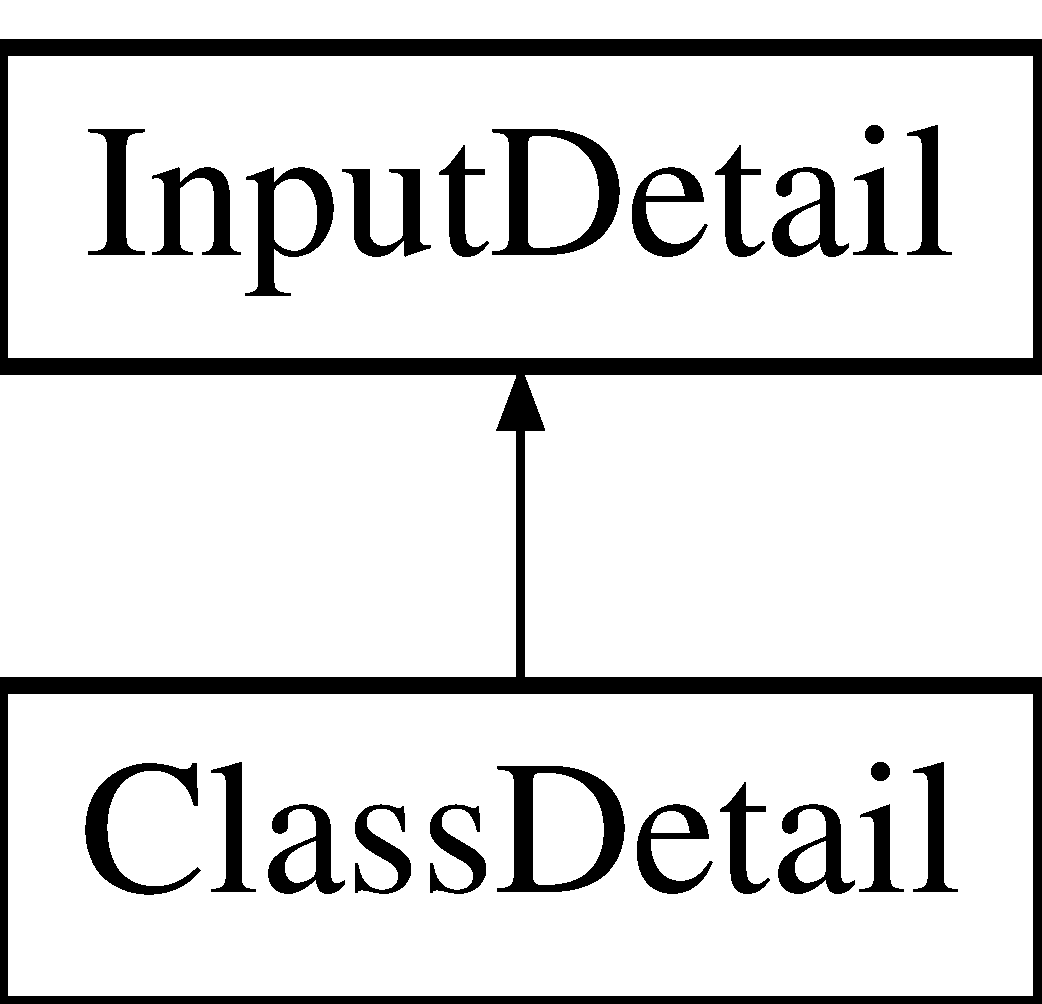
\includegraphics[height=2.000000cm]{classClassDetail}
\end{center}
\end{figure}
\subsection*{Public Member Functions}
\begin{DoxyCompactItemize}
\item 
\hyperlink{classClassDetail_a70975c4ff964e21958e31f2020cdc643}{Class\-Detail} ()
\begin{DoxyCompactList}\small\item\em Constructor. \end{DoxyCompactList}\item 
void \hyperlink{classClassDetail_a2e2384f482bb2dca5f2d8a1c27491ae9}{Set\-Default\-Value} ()
\begin{DoxyCompactList}\small\item\em Setting default values of text fields (classname, subject name, subject code) \end{DoxyCompactList}\item 
void \hyperlink{classClassDetail_a360bb591c7b1559d1b6bac0609dbad1e}{Project\-Type} ()
\begin{DoxyCompactList}\small\item\em For reading project type ie old or new then calling Old\-Project and New\-Project func. accord to that. \end{DoxyCompactList}\item 
void \hyperlink{classClassDetail_af8cb05bf1c3d5581edddcdab96def081}{Old\-Project} ()
\begin{DoxyCompactList}\small\item\em This func. is called is project type = Old. \end{DoxyCompactList}\item 
void \hyperlink{classClassDetail_a521c8e315fa844a04932382ae85335bf}{New\-Project} ()
\begin{DoxyCompactList}\small\item\em This func tis called if Project\-Type = New. \end{DoxyCompactList}\item 
void \hyperlink{classClassDetail_a645fe4306391def818cdadbdc3febbf7}{Class\-Detail\-Page} (string \hyperlink{classInputDetail_a1abb16cd695678c3fa05e3c812823fee}{msg}=\char`\"{}\char`\"{})
\begin{DoxyCompactList}\small\item\em function for displaying html page for class details \end{DoxyCompactList}\item 
\hyperlink{classClassDetail_a2aeaf33b0a277a897aad308cffde211a}{$\sim$\-Class\-Detail} ()
\begin{DoxyCompactList}\small\item\em Destructor. \end{DoxyCompactList}\end{DoxyCompactItemize}
\subsection*{Protected Attributes}
\begin{DoxyCompactItemize}
\item 
\hypertarget{classClassDetail_af920fe4a369c37b9b48b1c4a5451b99c}{\hyperlink{classProjectDetail}{Project\-Detail} {\bfseries project}}\label{classClassDetail_af920fe4a369c37b9b48b1c4a5451b99c}

\item 
\hypertarget{classClassDetail_ae990299c6643a8d4f958585e790d0dc8}{S\-T\-R\-I\-N\-G\-\_\-\-V\-E\-C {\bfseries value}}\label{classClassDetail_ae990299c6643a8d4f958585e790d0dc8}

\end{DoxyCompactItemize}


\subsection{Detailed Description}
For getting class details nd reading projectdetail. 

Include \hyperlink{class_8h}{class.\-h}

Include \hyperlink{project_8h_source}{project.\-h} 

Definition at line 30 of file class.\-h.



\subsection{Constructor \& Destructor Documentation}
\hypertarget{classClassDetail_a70975c4ff964e21958e31f2020cdc643}{\index{Class\-Detail@{Class\-Detail}!Class\-Detail@{Class\-Detail}}
\index{Class\-Detail@{Class\-Detail}!ClassDetail@{Class\-Detail}}
\subsubsection[{Class\-Detail}]{\setlength{\rightskip}{0pt plus 5cm}Class\-Detail\-::\-Class\-Detail (
\begin{DoxyParamCaption}
{}
\end{DoxyParamCaption}
)}}\label{classClassDetail_a70975c4ff964e21958e31f2020cdc643}


Constructor. 

Constructor 

Definition at line 27 of file class.\-cc.

\hypertarget{classClassDetail_a2aeaf33b0a277a897aad308cffde211a}{\index{Class\-Detail@{Class\-Detail}!$\sim$\-Class\-Detail@{$\sim$\-Class\-Detail}}
\index{$\sim$\-Class\-Detail@{$\sim$\-Class\-Detail}!ClassDetail@{Class\-Detail}}
\subsubsection[{$\sim$\-Class\-Detail}]{\setlength{\rightskip}{0pt plus 5cm}Class\-Detail\-::$\sim$\-Class\-Detail (
\begin{DoxyParamCaption}
{}
\end{DoxyParamCaption}
)}}\label{classClassDetail_a2aeaf33b0a277a897aad308cffde211a}


Destructor. 

D\-Estructor 

Definition at line 319 of file class.\-cc.



\subsection{Member Function Documentation}
\hypertarget{classClassDetail_a645fe4306391def818cdadbdc3febbf7}{\index{Class\-Detail@{Class\-Detail}!Class\-Detail\-Page@{Class\-Detail\-Page}}
\index{Class\-Detail\-Page@{Class\-Detail\-Page}!ClassDetail@{Class\-Detail}}
\subsubsection[{Class\-Detail\-Page}]{\setlength{\rightskip}{0pt plus 5cm}void Class\-Detail\-::\-Class\-Detail\-Page (
\begin{DoxyParamCaption}
\item[{string}]{msg = {\ttfamily \char`\"{}\char`\"{}}}
\end{DoxyParamCaption}
)}}\label{classClassDetail_a645fe4306391def818cdadbdc3febbf7}


function for displaying html page for class details 

Class detail page


\begin{DoxyParams}{Parameters}
{\em msg} & For displaying error message if any \\
\hline
\end{DoxyParams}


Definition at line 181 of file class.\-cc.

\hypertarget{classClassDetail_a521c8e315fa844a04932382ae85335bf}{\index{Class\-Detail@{Class\-Detail}!New\-Project@{New\-Project}}
\index{New\-Project@{New\-Project}!ClassDetail@{Class\-Detail}}
\subsubsection[{New\-Project}]{\setlength{\rightskip}{0pt plus 5cm}void Class\-Detail\-::\-New\-Project (
\begin{DoxyParamCaption}
{}
\end{DoxyParamCaption}
)}}\label{classClassDetail_a521c8e315fa844a04932382ae85335bf}


This func tis called if Project\-Type = New. 

New project $<$ If project\-Name already exists 

Definition at line 96 of file class.\-cc.

\hypertarget{classClassDetail_af8cb05bf1c3d5581edddcdab96def081}{\index{Class\-Detail@{Class\-Detail}!Old\-Project@{Old\-Project}}
\index{Old\-Project@{Old\-Project}!ClassDetail@{Class\-Detail}}
\subsubsection[{Old\-Project}]{\setlength{\rightskip}{0pt plus 5cm}void Class\-Detail\-::\-Old\-Project (
\begin{DoxyParamCaption}
{}
\end{DoxyParamCaption}
)}}\label{classClassDetail_af8cb05bf1c3d5581edddcdab96def081}


This func. is called is project type = Old. 

Existing project $<$ If project\-Name already exists 

Definition at line 132 of file class.\-cc.

\hypertarget{classClassDetail_a360bb591c7b1559d1b6bac0609dbad1e}{\index{Class\-Detail@{Class\-Detail}!Project\-Type@{Project\-Type}}
\index{Project\-Type@{Project\-Type}!ClassDetail@{Class\-Detail}}
\subsubsection[{Project\-Type}]{\setlength{\rightskip}{0pt plus 5cm}void Class\-Detail\-::\-Project\-Type (
\begin{DoxyParamCaption}
{}
\end{DoxyParamCaption}
)}}\label{classClassDetail_a360bb591c7b1559d1b6bac0609dbad1e}


For reading project type ie old or new then calling Old\-Project and New\-Project func. accord to that. 

Type of project 

Definition at line 49 of file class.\-cc.

\hypertarget{classClassDetail_a2e2384f482bb2dca5f2d8a1c27491ae9}{\index{Class\-Detail@{Class\-Detail}!Set\-Default\-Value@{Set\-Default\-Value}}
\index{Set\-Default\-Value@{Set\-Default\-Value}!ClassDetail@{Class\-Detail}}
\subsubsection[{Set\-Default\-Value}]{\setlength{\rightskip}{0pt plus 5cm}void Class\-Detail\-::\-Set\-Default\-Value (
\begin{DoxyParamCaption}
{}
\end{DoxyParamCaption}
)}}\label{classClassDetail_a2e2384f482bb2dca5f2d8a1c27491ae9}


Setting default values of text fields (classname, subject name, subject code) 

Set default values 

Definition at line 77 of file class.\-cc.



The documentation for this class was generated from the following files\-:\begin{DoxyCompactItemize}
\item 
frontend/src/header/\hyperlink{class_8h}{class.\-h}\item 
frontend/src/\hyperlink{class_8cc}{class.\-cc}\end{DoxyCompactItemize}

\hypertarget{classDatabase}{\section{Database Class Reference}
\label{classDatabase}\index{Database@{Database}}
}


{\ttfamily \#include $<$database.\-h$>$}

\subsection*{Public Member Functions}
\begin{DoxyCompactItemize}
\item 
\hyperlink{classDatabase_a4703c80e6969d33565ea340f768fdadf}{Database} ()
\item 
void \hyperlink{classDatabase_aec3d0f84e49a58a59f254c90193c1303}{Select\-Query} (string column, string table, vector$<$ string $>$ \&result)
\item 
void \hyperlink{classDatabase_a958467134aa40db133cdf6d46ab52c86}{Select\-Query} (string column, string table, string \&result, string where)
\item 
void \hyperlink{classDatabase_a6fb9e249cb97830af86c00804bb209a2}{Select\-Column} (string query, vector$<$ string $>$ \&result)
\item 
void \hyperlink{classDatabase_a20f7ccadac8f3b67d4344f7da4594eda}{Select\-Project\-I\-D} (string \&project\-I\-D)
\item 
void \hyperlink{classDatabase_a7070d93bf44c5f90504944f54607b9b0}{Insert\-User} (string user\-Email\-I\-D, string user\-Password)
\item 
void \hyperlink{classDatabase_a63d8c1af7507b1dcdc81a411f9a0b4b4}{Insert\-Query} (string query)
\item 
void \hyperlink{classDatabase_a513326ea43b2455177731fbc92c4bf4f}{Insert\-Query} (string column, string value, string table)
\item 
void \hyperlink{classDatabase_a478f862bd338a92b13c2899bb4e28843}{Insert\-Session} (string email\-I\-D, string session\-I\-D)
\item 
void \hyperlink{classDatabase_aae19d9dac16779519f94cc68e29cb57d}{Insert\-Project\-Name} (string email\-I\-D, string project\-Name)
\item 
void \hyperlink{classDatabase_ad6af2dc859cda41dcbdad9cd51f5c38b}{Insert\-Total\-Classes} (string project\-I\-D, string total\-Classes)
\item 
void \hyperlink{classDatabase_a45deae7ea496fccefb9bccd75ea5578a}{Insert\-Class\-Detail} (string project\-I\-D, string class\-Name, string total\-Subjects, string subject\-Name, string subject\-Code)
\item 
void \hyperlink{classDatabase_a8e52c1b853b6f1d96cf7053f0268838d}{Insert\-Total\-Centres} (string project\-I\-D, string total\-Centre)
\item 
void \hyperlink{classDatabase_a8b248d14e1cb2fc4ba2c9da313f385cb}{Insert\-Room\-Detail} (string project\-I\-D, string centre\-Name, string room\-No, string rows, string columns)
\item 
void \hyperlink{classDatabase_a6cd1b1181fb636aff93ba43f0fcd2764}{Insert\-Total\-Rooms} (string project\-I\-D, string centre\-Name, string totalrooms)
\item 
void \hyperlink{classDatabase_a0a1ec932aafeef96637d5ee68ac7898b}{Insert\-Exam\-Detail} (string project\-I\-D, string exam\-Name, string exam\-Date, string exam\-Time, string exam\-Venue)
\item 
void \hyperlink{classDatabase_a6015ae56eb561f579e573be709ef434c}{Insert\-Strategy} (string project\-I\-D, string strategy)
\item 
\hyperlink{classDatabase_a84d399a2ad58d69daab9b05330e1316d}{$\sim$\-Database} ()
\end{DoxyCompactItemize}
\subsection*{Protected Attributes}
\begin{DoxyCompactItemize}
\item 
M\-Y\-S\-Q\-L $\ast$ \hyperlink{classDatabase_aa232b806b05ef654cd5579bca5f1dbad}{connect}
\item 
\hypertarget{classDatabase_ad5921cd2f70d0c22895f2cc5542ab4d7}{M\-Y\-S\-Q\-L\-\_\-\-R\-E\-S $\ast$ {\bfseries res\-\_\-set}}\label{classDatabase_ad5921cd2f70d0c22895f2cc5542ab4d7}

\item 
\hypertarget{classDatabase_a71ad7ae59677936d2ca6666f9de9df40}{M\-Y\-S\-Q\-L\-\_\-\-R\-O\-W {\bfseries row}}\label{classDatabase_a71ad7ae59677936d2ca6666f9de9df40}

\item 
unsigned int \hyperlink{classDatabase_a02965883689dd1d8007c86cebf6df89e}{numrows}
\item 
string \hyperlink{classDatabase_acd64ff0e98b28cd1c6928a1236634521}{t\-Login}
\item 
\hypertarget{classDatabase_aa8ec817b6216079c8e541ec80c8bd4fa}{string {\bfseries t\-Register}}\label{classDatabase_aa8ec817b6216079c8e541ec80c8bd4fa}

\item 
\hypertarget{classDatabase_a62dd3ad69a4a07e66b412e276049ea48}{string {\bfseries t\-Project\-Detail}}\label{classDatabase_a62dd3ad69a4a07e66b412e276049ea48}

\item 
\hypertarget{classDatabase_a1b3174ab4ae9b3cb80448d48817375be}{int {\bfseries i}}\label{classDatabase_a1b3174ab4ae9b3cb80448d48817375be}

\item 
\hypertarget{classDatabase_a5b4fd605238ca66878959f5f3ba647f2}{int {\bfseries j}}\label{classDatabase_a5b4fd605238ca66878959f5f3ba647f2}

\item 
\hypertarget{classDatabase_a851daa5b233ce54d75873631b7b2167a}{string {\bfseries query}}\label{classDatabase_a851daa5b233ce54d75873631b7b2167a}

\end{DoxyCompactItemize}


\subsection{Detailed Description}
-\/-\/-\/-\/-\/-\/-\/-\/-\/-\/-\/-\/-\/-\/-\/-\/-\/-\/-\/-\/-\/-\/-\/-\/-\/-\/-\/-\/-\/-\/-\/-\/-\/-\/-\/-\/-\/-\/-\/-\/-\/-\/-\/-\/-\/-\/-\/-\/-\/-\/-\/-\/-\/-\/-\/-\/-\/-\/-\/-\/-\/-\/-\/-\/-\/-\/-\/ Include \hyperlink{header_8h_source}{header.\-h} and \hyperlink{database_8h_source}{database.\-h} ------------------------------------------------------------------ =================================================================== Class\-: \hyperlink{classDatabase}{Database} Description\-: \hyperlink{classDatabase}{Database} class for database accessability =================================================================== 

Definition at line 34 of file database.\-h.



\subsection{Constructor \& Destructor Documentation}
\hypertarget{classDatabase_a4703c80e6969d33565ea340f768fdadf}{\index{Database@{Database}!Database@{Database}}
\index{Database@{Database}!Database@{Database}}
\subsubsection[{Database}]{\setlength{\rightskip}{0pt plus 5cm}Database\-::\-Database (
\begin{DoxyParamCaption}
{}
\end{DoxyParamCaption}
)}}\label{classDatabase_a4703c80e6969d33565ea340f768fdadf}
\hyperlink{classDatabase}{Database} Constructor

-\/-\/-\/-\/-\/-\/-\/-\/-\/-\/-\/-\/-\/-\/-\/-\/-\/-\/-\/-\/-\/-\/-\/-\/-\/-\/-\/-\/-\/-\/-\/-\/-\/-\/-\/-\/-\/-\/-\/-\/-\/-\/-\/-\/-\/-\/-\/-\/-\/-\/-\/-\/-\/-\/-\/-\/-\/-\/-\/-\/-\/-\/-\/-\/-\/-\/-\/ Include \hyperlink{database_8h_source}{database.\-h} file local header file(declaration of class) ------------------------------------------------------------------ -\/-\/-\/-\/-\/-\/-\/-\/-\/-\/-\/-\/-\/-\/-\/-\/-\/-\/-\/-\/-\/-\/-\/-\/-\/-\/-\/-\/-\/-\/-\/-\/-\/-\/-\/-\/-\/-\/-\/-\/-\/-\/-\/-\/-\/-\/-\/-\/-\/-\/-\/-\/-\/-\/-\/-\/-\/-\/-\/-\/-\/-\/-\/-\/-\/-\/-\/-\/ Class\-: \hyperlink{classDatabase}{Database} Method\-: \hyperlink{classDatabase}{Database} \-:\-: \hyperlink{classDatabase_a4703c80e6969d33565ea340f768fdadf}{Database()} Description\-: Constructor to initialize database conectivity -\/-\/-\/-\/-\/-\/-\/-\/-\/-\/-\/-\/-\/-\/-\/-\/-\/-\/-\/-\/-\/-\/-\/-\/-\/-\/-\/-\/-\/-\/-\/-\/-\/-\/-\/-\/-\/-\/-\/-\/-\/-\/-\/-\/-\/-\/-\/-\/-\/-\/-\/-\/-\/-\/-\/-\/-\/-\/-\/-\/-\/-\/-\/-\/-\/-\/-\/-\/ 

Definition at line 33 of file database.\-cc.

\hypertarget{classDatabase_a84d399a2ad58d69daab9b05330e1316d}{\index{Database@{Database}!$\sim$\-Database@{$\sim$\-Database}}
\index{$\sim$\-Database@{$\sim$\-Database}!Database@{Database}}
\subsubsection[{$\sim$\-Database}]{\setlength{\rightskip}{0pt plus 5cm}Database\-::$\sim$\-Database (
\begin{DoxyParamCaption}
{}
\end{DoxyParamCaption}
)}}\label{classDatabase_a84d399a2ad58d69daab9b05330e1316d}
Select last project Id of project name \hyperlink{classDatabase}{Database} Destructor

-\/-\/-\/-\/-\/-\/-\/-\/-\/-\/-\/-\/-\/-\/-\/-\/-\/-\/-\/-\/-\/-\/-\/-\/-\/-\/-\/-\/-\/-\/-\/-\/-\/-\/-\/-\/-\/-\/-\/-\/-\/-\/-\/-\/-\/-\/-\/-\/-\/-\/-\/-\/-\/-\/-\/-\/-\/-\/-\/-\/-\/-\/-\/-\/-\/-\/-\/-\/ Class\-: \hyperlink{classDatabase}{Database} Method\-: \hyperlink{classDatabase}{Database} \-:\-: \hyperlink{classDatabase_a84d399a2ad58d69daab9b05330e1316d}{$\sim$\-Database()} Description\-: Destructor for closing database connectivity -\/-\/-\/-\/-\/-\/-\/-\/-\/-\/-\/-\/-\/-\/-\/-\/-\/-\/-\/-\/-\/-\/-\/-\/-\/-\/-\/-\/-\/-\/-\/-\/-\/-\/-\/-\/-\/-\/-\/-\/-\/-\/-\/-\/-\/-\/-\/-\/-\/-\/-\/-\/-\/-\/-\/-\/-\/-\/-\/-\/-\/-\/-\/-\/-\/-\/-\/-\/ 

Definition at line 401 of file database.\-cc.



\subsection{Member Function Documentation}
\hypertarget{classDatabase_a45deae7ea496fccefb9bccd75ea5578a}{\index{Database@{Database}!Insert\-Class\-Detail@{Insert\-Class\-Detail}}
\index{Insert\-Class\-Detail@{Insert\-Class\-Detail}!Database@{Database}}
\subsubsection[{Insert\-Class\-Detail}]{\setlength{\rightskip}{0pt plus 5cm}void Database\-::\-Insert\-Class\-Detail (
\begin{DoxyParamCaption}
\item[{string}]{project\-I\-D, }
\item[{string}]{class\-Name, }
\item[{string}]{total\-Subjects, }
\item[{string}]{subject\-Name, }
\item[{string}]{subject\-Code}
\end{DoxyParamCaption}
)}}\label{classDatabase_a45deae7ea496fccefb9bccd75ea5578a}
Insert into \hyperlink{classClassDetail}{Class\-Detail}

--------------------------------------------------------------------\par
 Class\-: \hyperlink{classDatabase}{Database} \par
 Method\-: \hyperlink{classDatabase}{Database} \-:\-: Insert\-Class\-Detail(project\-I\-D, class\-Name, subject\-Name, subject\-Code) \par
 Description\-: Inserting class detail into table \par
 -\/-\/-\/-\/-\/-\/-\/-\/-\/-\/-\/-\/-\/-\/-\/-\/-\/-\/-\/-\/-\/-\/-\/-\/-\/-\/-\/-\/-\/-\/-\/-\/-\/-\/-\/-\/-\/-\/-\/-\/-\/-\/-\/-\/-\/-\/-\/-\/-\/-\/-\/-\/-\/-\/-\/-\/-\/-\/-\/-\/-\/-\/-\/-\/-\/-\/-\/-\/ 

Definition at line 258 of file database.\-cc.

\hypertarget{classDatabase_a0a1ec932aafeef96637d5ee68ac7898b}{\index{Database@{Database}!Insert\-Exam\-Detail@{Insert\-Exam\-Detail}}
\index{Insert\-Exam\-Detail@{Insert\-Exam\-Detail}!Database@{Database}}
\subsubsection[{Insert\-Exam\-Detail}]{\setlength{\rightskip}{0pt plus 5cm}void Database\-::\-Insert\-Exam\-Detail (
\begin{DoxyParamCaption}
\item[{string}]{project\-I\-D, }
\item[{string}]{exam\-Name, }
\item[{string}]{exam\-Date, }
\item[{string}]{exam\-Time, }
\item[{string}]{exam\-Venue}
\end{DoxyParamCaption}
)}}\label{classDatabase_a0a1ec932aafeef96637d5ee68ac7898b}
Insert into exam detail

--------------------------------------------------------------------\par
 Class\-: \hyperlink{classDatabase}{Database} \par
 Method\-: \hyperlink{classDatabase}{Database} \-:\-: Insert\-Total\-Rooms(project\-I\-D, exam\-Name, exam\-Date, exam\-Time, exam\-Venue) \par
 Description\-: store data into exam detail \par
 -\/-\/-\/-\/-\/-\/-\/-\/-\/-\/-\/-\/-\/-\/-\/-\/-\/-\/-\/-\/-\/-\/-\/-\/-\/-\/-\/-\/-\/-\/-\/-\/-\/-\/-\/-\/-\/-\/-\/-\/-\/-\/-\/-\/-\/-\/-\/-\/-\/-\/-\/-\/-\/-\/-\/-\/-\/-\/-\/-\/-\/-\/-\/-\/-\/-\/-\/-\/ 

Definition at line 355 of file database.\-cc.

\hypertarget{classDatabase_aae19d9dac16779519f94cc68e29cb57d}{\index{Database@{Database}!Insert\-Project\-Name@{Insert\-Project\-Name}}
\index{Insert\-Project\-Name@{Insert\-Project\-Name}!Database@{Database}}
\subsubsection[{Insert\-Project\-Name}]{\setlength{\rightskip}{0pt plus 5cm}void Database\-::\-Insert\-Project\-Name (
\begin{DoxyParamCaption}
\item[{string}]{email\-I\-D, }
\item[{string}]{project\-Name}
\end{DoxyParamCaption}
)}}\label{classDatabase_aae19d9dac16779519f94cc68e29cb57d}
Insert Project detail into Project\-Name table

--------------------------------------------------------------------\par
 Class\-: \hyperlink{classDatabase}{Database} \par
 Method\-: \hyperlink{classDatabase}{Database} \-:\-: Insert\-Into\-Project\-Name() \par
 Description\-: Insert project name into Project\-Name table \par
 -\/-\/-\/-\/-\/-\/-\/-\/-\/-\/-\/-\/-\/-\/-\/-\/-\/-\/-\/-\/-\/-\/-\/-\/-\/-\/-\/-\/-\/-\/-\/-\/-\/-\/-\/-\/-\/-\/-\/-\/-\/-\/-\/-\/-\/-\/-\/-\/-\/-\/-\/-\/-\/-\/-\/-\/-\/-\/-\/-\/-\/-\/-\/-\/-\/-\/-\/-\/ 

Definition at line 217 of file database.\-cc.

\hypertarget{classDatabase_a63d8c1af7507b1dcdc81a411f9a0b4b4}{\index{Database@{Database}!Insert\-Query@{Insert\-Query}}
\index{Insert\-Query@{Insert\-Query}!Database@{Database}}
\subsubsection[{Insert\-Query}]{\setlength{\rightskip}{0pt plus 5cm}void Database\-::\-Insert\-Query (
\begin{DoxyParamCaption}
\item[{string}]{query}
\end{DoxyParamCaption}
)}}\label{classDatabase_a63d8c1af7507b1dcdc81a411f9a0b4b4}
Insert query with one argument

--------------------------------------------------------------------\par
 Class\-: \hyperlink{classDatabase}{Database} \par
 Method\-: \hyperlink{classDatabase}{Database} \-:\-: \hyperlink{classDatabase_a63d8c1af7507b1dcdc81a411f9a0b4b4}{Insert\-Query(string query)} \par
 Description\-: Insrting value in database \par
 -\/-\/-\/-\/-\/-\/-\/-\/-\/-\/-\/-\/-\/-\/-\/-\/-\/-\/-\/-\/-\/-\/-\/-\/-\/-\/-\/-\/-\/-\/-\/-\/-\/-\/-\/-\/-\/-\/-\/-\/-\/-\/-\/-\/-\/-\/-\/-\/-\/-\/-\/-\/-\/-\/-\/-\/-\/-\/-\/-\/-\/-\/-\/-\/-\/-\/-\/-\/ 

Definition at line 136 of file database.\-cc.

\hypertarget{classDatabase_a513326ea43b2455177731fbc92c4bf4f}{\index{Database@{Database}!Insert\-Query@{Insert\-Query}}
\index{Insert\-Query@{Insert\-Query}!Database@{Database}}
\subsubsection[{Insert\-Query}]{\setlength{\rightskip}{0pt plus 5cm}void Database\-::\-Insert\-Query (
\begin{DoxyParamCaption}
\item[{string}]{column, }
\item[{string}]{value, }
\item[{string}]{table}
\end{DoxyParamCaption}
)}}\label{classDatabase_a513326ea43b2455177731fbc92c4bf4f}
Insert Query for adding value in one column

--------------------------------------------------------------------\par
 Class\-: \hyperlink{classDatabase}{Database} \par
 Method\-: \hyperlink{classDatabase}{Database} \-:\-: Insert\-Query(string column, string value, string table) \par
 Description\-: For inserting values in database \par
 -\/-\/-\/-\/-\/-\/-\/-\/-\/-\/-\/-\/-\/-\/-\/-\/-\/-\/-\/-\/-\/-\/-\/-\/-\/-\/-\/-\/-\/-\/-\/-\/-\/-\/-\/-\/-\/-\/-\/-\/-\/-\/-\/-\/-\/-\/-\/-\/-\/-\/-\/-\/-\/-\/-\/-\/-\/-\/-\/-\/-\/-\/-\/-\/-\/-\/-\/-\/ 

Definition at line 153 of file database.\-cc.

\hypertarget{classDatabase_a8b248d14e1cb2fc4ba2c9da313f385cb}{\index{Database@{Database}!Insert\-Room\-Detail@{Insert\-Room\-Detail}}
\index{Insert\-Room\-Detail@{Insert\-Room\-Detail}!Database@{Database}}
\subsubsection[{Insert\-Room\-Detail}]{\setlength{\rightskip}{0pt plus 5cm}void Database\-::\-Insert\-Room\-Detail (
\begin{DoxyParamCaption}
\item[{string}]{project\-I\-D, }
\item[{string}]{centre\-Name, }
\item[{string}]{room\-No, }
\item[{string}]{rows, }
\item[{string}]{columns}
\end{DoxyParamCaption}
)}}\label{classDatabase_a8b248d14e1cb2fc4ba2c9da313f385cb}
Insert into room\-Detail table

--------------------------------------------------------------------\par
 Class\-: \hyperlink{classDatabase}{Database} \par
 Method\-: \hyperlink{classDatabase}{Database} \-:\-: Insert\-Room\-Detail(project\-I\-D, centre\-Name, room\-No, rows, columns) \par
 Description\-: Inserting room detail into table \par
 -\/-\/-\/-\/-\/-\/-\/-\/-\/-\/-\/-\/-\/-\/-\/-\/-\/-\/-\/-\/-\/-\/-\/-\/-\/-\/-\/-\/-\/-\/-\/-\/-\/-\/-\/-\/-\/-\/-\/-\/-\/-\/-\/-\/-\/-\/-\/-\/-\/-\/-\/-\/-\/-\/-\/-\/-\/-\/-\/-\/-\/-\/-\/-\/-\/-\/-\/-\/ 

Definition at line 303 of file database.\-cc.

\hypertarget{classDatabase_a478f862bd338a92b13c2899bb4e28843}{\index{Database@{Database}!Insert\-Session@{Insert\-Session}}
\index{Insert\-Session@{Insert\-Session}!Database@{Database}}
\subsubsection[{Insert\-Session}]{\setlength{\rightskip}{0pt plus 5cm}void Database\-::\-Insert\-Session (
\begin{DoxyParamCaption}
\item[{string}]{email\-I\-D, }
\item[{string}]{session\-I\-D}
\end{DoxyParamCaption}
)}}\label{classDatabase_a478f862bd338a92b13c2899bb4e28843}
Insert into Session table

--------------------------------------------------------------------\par
 Class\-: \hyperlink{classDatabase}{Database} \par
 Method\-: \hyperlink{classDatabase}{Database} \-:\-: Insert\-Into\-Session(string email\-I\-D, string session\-I\-D) \par
 Description\-: Inserting Session information in database \par
 -\/-\/-\/-\/-\/-\/-\/-\/-\/-\/-\/-\/-\/-\/-\/-\/-\/-\/-\/-\/-\/-\/-\/-\/-\/-\/-\/-\/-\/-\/-\/-\/-\/-\/-\/-\/-\/-\/-\/-\/-\/-\/-\/-\/-\/-\/-\/-\/-\/-\/-\/-\/-\/-\/-\/-\/-\/-\/-\/-\/-\/-\/-\/-\/-\/-\/-\/-\/ 

Definition at line 198 of file database.\-cc.

\hypertarget{classDatabase_a6015ae56eb561f579e573be709ef434c}{\index{Database@{Database}!Insert\-Strategy@{Insert\-Strategy}}
\index{Insert\-Strategy@{Insert\-Strategy}!Database@{Database}}
\subsubsection[{Insert\-Strategy}]{\setlength{\rightskip}{0pt plus 5cm}void Database\-::\-Insert\-Strategy (
\begin{DoxyParamCaption}
\item[{string}]{project\-I\-D, }
\item[{string}]{strategy}
\end{DoxyParamCaption}
)}}\label{classDatabase_a6015ae56eb561f579e573be709ef434c}
Insert into strategy

--------------------------------------------------------------------\par
 Class\-: \hyperlink{classDatabase}{Database} \par
 Method\-: \hyperlink{classDatabase}{Database} \-:\-: Insert\-Total\-Rooms(project\-I\-D, strategy) \par
 Description\-: Strategy value into table \par
 -\/-\/-\/-\/-\/-\/-\/-\/-\/-\/-\/-\/-\/-\/-\/-\/-\/-\/-\/-\/-\/-\/-\/-\/-\/-\/-\/-\/-\/-\/-\/-\/-\/-\/-\/-\/-\/-\/-\/-\/-\/-\/-\/-\/-\/-\/-\/-\/-\/-\/-\/-\/-\/-\/-\/-\/-\/-\/-\/-\/-\/-\/-\/-\/-\/-\/-\/-\/ 

Definition at line 382 of file database.\-cc.

\hypertarget{classDatabase_a8e52c1b853b6f1d96cf7053f0268838d}{\index{Database@{Database}!Insert\-Total\-Centres@{Insert\-Total\-Centres}}
\index{Insert\-Total\-Centres@{Insert\-Total\-Centres}!Database@{Database}}
\subsubsection[{Insert\-Total\-Centres}]{\setlength{\rightskip}{0pt plus 5cm}void Database\-::\-Insert\-Total\-Centres (
\begin{DoxyParamCaption}
\item[{string}]{project\-I\-D, }
\item[{string}]{total\-Centre}
\end{DoxyParamCaption}
)}}\label{classDatabase_a8e52c1b853b6f1d96cf7053f0268838d}
Insert into totalcentres

--------------------------------------------------------------------\par
 Class\-: \hyperlink{classDatabase}{Database} \par
 Method\-: \hyperlink{classDatabase}{Database} \-:\-: Inserttotal\-Centres(project\-I\-D,totalcentre) \par
 Description\-: Inserting into table total centrres \par
 -\/-\/-\/-\/-\/-\/-\/-\/-\/-\/-\/-\/-\/-\/-\/-\/-\/-\/-\/-\/-\/-\/-\/-\/-\/-\/-\/-\/-\/-\/-\/-\/-\/-\/-\/-\/-\/-\/-\/-\/-\/-\/-\/-\/-\/-\/-\/-\/-\/-\/-\/-\/-\/-\/-\/-\/-\/-\/-\/-\/-\/-\/-\/-\/-\/-\/-\/-\/ 

Definition at line 282 of file database.\-cc.

\hypertarget{classDatabase_ad6af2dc859cda41dcbdad9cd51f5c38b}{\index{Database@{Database}!Insert\-Total\-Classes@{Insert\-Total\-Classes}}
\index{Insert\-Total\-Classes@{Insert\-Total\-Classes}!Database@{Database}}
\subsubsection[{Insert\-Total\-Classes}]{\setlength{\rightskip}{0pt plus 5cm}void Database\-::\-Insert\-Total\-Classes (
\begin{DoxyParamCaption}
\item[{string}]{project\-I\-D, }
\item[{string}]{total\-Classes}
\end{DoxyParamCaption}
)}}\label{classDatabase_ad6af2dc859cda41dcbdad9cd51f5c38b}
Insert Into Total\-Classes

--------------------------------------------------------------------\par
 Class\-: \hyperlink{classDatabase}{Database} \par
 Method\-: \hyperlink{classDatabase}{Database} \-:\-: Insert\-Total\-Classes(project\-I\-D, total\-Classes) \par
 Description\-: Inserting total classes into table with project I\-D \par
 -\/-\/-\/-\/-\/-\/-\/-\/-\/-\/-\/-\/-\/-\/-\/-\/-\/-\/-\/-\/-\/-\/-\/-\/-\/-\/-\/-\/-\/-\/-\/-\/-\/-\/-\/-\/-\/-\/-\/-\/-\/-\/-\/-\/-\/-\/-\/-\/-\/-\/-\/-\/-\/-\/-\/-\/-\/-\/-\/-\/-\/-\/-\/-\/-\/-\/-\/-\/ 

Definition at line 237 of file database.\-cc.

\hypertarget{classDatabase_a6cd1b1181fb636aff93ba43f0fcd2764}{\index{Database@{Database}!Insert\-Total\-Rooms@{Insert\-Total\-Rooms}}
\index{Insert\-Total\-Rooms@{Insert\-Total\-Rooms}!Database@{Database}}
\subsubsection[{Insert\-Total\-Rooms}]{\setlength{\rightskip}{0pt plus 5cm}void Database\-::\-Insert\-Total\-Rooms (
\begin{DoxyParamCaption}
\item[{string}]{project\-I\-D, }
\item[{string}]{centre\-Name, }
\item[{string}]{total\-Rooms}
\end{DoxyParamCaption}
)}}\label{classDatabase_a6cd1b1181fb636aff93ba43f0fcd2764}
Insert Into Total\-Rooms

--------------------------------------------------------------------\par
 Class\-: \hyperlink{classDatabase}{Database} \par
 Method\-: \hyperlink{classDatabase}{Database} \-:\-: Insert\-Total\-Rooms(project\-I\-D, centre\-Name, totalrooms) \par
 Description\-: Inserting into total rooms \par
 -\/-\/-\/-\/-\/-\/-\/-\/-\/-\/-\/-\/-\/-\/-\/-\/-\/-\/-\/-\/-\/-\/-\/-\/-\/-\/-\/-\/-\/-\/-\/-\/-\/-\/-\/-\/-\/-\/-\/-\/-\/-\/-\/-\/-\/-\/-\/-\/-\/-\/-\/-\/-\/-\/-\/-\/-\/-\/-\/-\/-\/-\/-\/-\/-\/-\/-\/-\/ 

Definition at line 331 of file database.\-cc.

\hypertarget{classDatabase_a7070d93bf44c5f90504944f54607b9b0}{\index{Database@{Database}!Insert\-User@{Insert\-User}}
\index{Insert\-User@{Insert\-User}!Database@{Database}}
\subsubsection[{Insert\-User}]{\setlength{\rightskip}{0pt plus 5cm}void Database\-::\-Insert\-User (
\begin{DoxyParamCaption}
\item[{string}]{user\-Email\-I\-D, }
\item[{string}]{user\-Password}
\end{DoxyParamCaption}
)}}\label{classDatabase_a7070d93bf44c5f90504944f54607b9b0}
For inserting new user in database

--------------------------------------------------------------------\par
 Class\-: \hyperlink{classDatabase}{Database} \par
 Method\-: \hyperlink{classDatabase}{Database} \-:\-: Insert\-Into\-User(string user\-Email\-I\-D, string user\-Password) \par
 Description\-: Inserting new user details into database \par
 -\/-\/-\/-\/-\/-\/-\/-\/-\/-\/-\/-\/-\/-\/-\/-\/-\/-\/-\/-\/-\/-\/-\/-\/-\/-\/-\/-\/-\/-\/-\/-\/-\/-\/-\/-\/-\/-\/-\/-\/-\/-\/-\/-\/-\/-\/-\/-\/-\/-\/-\/-\/-\/-\/-\/-\/-\/-\/-\/-\/-\/-\/-\/-\/-\/-\/-\/-\/ 

Definition at line 176 of file database.\-cc.

\hypertarget{classDatabase_a6fb9e249cb97830af86c00804bb209a2}{\index{Database@{Database}!Select\-Column@{Select\-Column}}
\index{Select\-Column@{Select\-Column}!Database@{Database}}
\subsubsection[{Select\-Column}]{\setlength{\rightskip}{0pt plus 5cm}void Database\-::\-Select\-Column (
\begin{DoxyParamCaption}
\item[{string}]{query, }
\item[{vector$<$ string $>$ \&}]{result}
\end{DoxyParamCaption}
)}}\label{classDatabase_a6fb9e249cb97830af86c00804bb209a2}
Seclect Column

--------------------------------------------------------------------\par
 Class\-: \hyperlink{classDatabase}{Database} \par
 Method\-: \hyperlink{classDatabase}{Database} \-:\-: Select\-Column \par
 Description\-: Select column from table \par
 -\/-\/-\/-\/-\/-\/-\/-\/-\/-\/-\/-\/-\/-\/-\/-\/-\/-\/-\/-\/-\/-\/-\/-\/-\/-\/-\/-\/-\/-\/-\/-\/-\/-\/-\/-\/-\/-\/-\/-\/-\/-\/-\/-\/-\/-\/-\/-\/-\/-\/-\/-\/-\/-\/-\/-\/-\/-\/-\/-\/-\/-\/-\/-\/-\/-\/-\/-\/ 

Definition at line 112 of file database.\-cc.

\hypertarget{classDatabase_a20f7ccadac8f3b67d4344f7da4594eda}{\index{Database@{Database}!Select\-Project\-I\-D@{Select\-Project\-I\-D}}
\index{Select\-Project\-I\-D@{Select\-Project\-I\-D}!Database@{Database}}
\subsubsection[{Select\-Project\-I\-D}]{\setlength{\rightskip}{0pt plus 5cm}void Database\-::\-Select\-Project\-I\-D (
\begin{DoxyParamCaption}
\item[{string \&}]{project\-I\-D}
\end{DoxyParamCaption}
)}}\label{classDatabase_a20f7ccadac8f3b67d4344f7da4594eda}
select project id from Project\-Name table 

Definition at line 95 of file database.\-cc.

\hypertarget{classDatabase_aec3d0f84e49a58a59f254c90193c1303}{\index{Database@{Database}!Select\-Query@{Select\-Query}}
\index{Select\-Query@{Select\-Query}!Database@{Database}}
\subsubsection[{Select\-Query}]{\setlength{\rightskip}{0pt plus 5cm}void Database\-::\-Select\-Query (
\begin{DoxyParamCaption}
\item[{string}]{column, }
\item[{string}]{table, }
\item[{vector$<$ string $>$ \&}]{result}
\end{DoxyParamCaption}
)}}\label{classDatabase_aec3d0f84e49a58a59f254c90193c1303}
For executing My\-S\-Q\-L query

--------------------------------------------------------------------\par
 Class\-: \hyperlink{classDatabase}{Database} \par
 Method\-: \hyperlink{classDatabase}{Database} \-:\-: Select\-Query(string column, string table) \par
 Description\-: Executing My\-S\-Q\-L Select Query and returns string value \par
 -\/-\/-\/-\/-\/-\/-\/-\/-\/-\/-\/-\/-\/-\/-\/-\/-\/-\/-\/-\/-\/-\/-\/-\/-\/-\/-\/-\/-\/-\/-\/-\/-\/-\/-\/-\/-\/-\/-\/-\/-\/-\/-\/-\/-\/-\/-\/-\/-\/-\/-\/-\/-\/-\/-\/-\/-\/-\/-\/-\/-\/-\/-\/-\/-\/-\/-\/-\/ 

Definition at line 59 of file database.\-cc.

\hypertarget{classDatabase_a958467134aa40db133cdf6d46ab52c86}{\index{Database@{Database}!Select\-Query@{Select\-Query}}
\index{Select\-Query@{Select\-Query}!Database@{Database}}
\subsubsection[{Select\-Query}]{\setlength{\rightskip}{0pt plus 5cm}void Database\-::\-Select\-Query (
\begin{DoxyParamCaption}
\item[{string}]{column, }
\item[{string}]{table, }
\item[{string \&}]{result, }
\item[{string}]{where}
\end{DoxyParamCaption}
)}}\label{classDatabase_a958467134aa40db133cdf6d46ab52c86}
Select query with where clause

--------------------------------------------------------------------\par
 Class\-: \hyperlink{classDatabase}{Database} \par
 Method\-: \hyperlink{classDatabase}{Database} \-:\-: Select\-Query(column, table, result, where) \par
 Description\-: Select column value with where clause \par
 -\/-\/-\/-\/-\/-\/-\/-\/-\/-\/-\/-\/-\/-\/-\/-\/-\/-\/-\/-\/-\/-\/-\/-\/-\/-\/-\/-\/-\/-\/-\/-\/-\/-\/-\/-\/-\/-\/-\/-\/-\/-\/-\/-\/-\/-\/-\/-\/-\/-\/-\/-\/-\/-\/-\/-\/-\/-\/-\/-\/-\/-\/-\/-\/-\/-\/-\/-\/ 

Definition at line 79 of file database.\-cc.



\subsection{Member Data Documentation}
\hypertarget{classDatabase_aa232b806b05ef654cd5579bca5f1dbad}{\index{Database@{Database}!connect@{connect}}
\index{connect@{connect}!Database@{Database}}
\subsubsection[{connect}]{\setlength{\rightskip}{0pt plus 5cm}M\-Y\-S\-Q\-L$\ast$ Database\-::connect\hspace{0.3cm}{\ttfamily [protected]}}}\label{classDatabase_aa232b806b05ef654cd5579bca5f1dbad}
My\-S\-Q\-L connectivity Variables 

Definition at line 38 of file database.\-h.

\hypertarget{classDatabase_a02965883689dd1d8007c86cebf6df89e}{\index{Database@{Database}!numrows@{numrows}}
\index{numrows@{numrows}!Database@{Database}}
\subsubsection[{numrows}]{\setlength{\rightskip}{0pt plus 5cm}unsigned int Database\-::numrows\hspace{0.3cm}{\ttfamily [protected]}}}\label{classDatabase_a02965883689dd1d8007c86cebf6df89e}
unsigned int variable 

Definition at line 43 of file database.\-h.

\hypertarget{classDatabase_acd64ff0e98b28cd1c6928a1236634521}{\index{Database@{Database}!t\-Login@{t\-Login}}
\index{t\-Login@{t\-Login}!Database@{Database}}
\subsubsection[{t\-Login}]{\setlength{\rightskip}{0pt plus 5cm}string Database\-::t\-Login\hspace{0.3cm}{\ttfamily [protected]}}}\label{classDatabase_acd64ff0e98b28cd1c6928a1236634521}
Table names t\-Tablename 

Definition at line 46 of file database.\-h.



The documentation for this class was generated from the following files\-:\begin{DoxyCompactItemize}
\item 
src/database.\-h\item 
src/database.\-cc\end{DoxyCompactItemize}

\hypertarget{classDataSheet}{\section{\-Data\-Sheet \-Class \-Reference}
\label{dd/dcc/classDataSheet}\index{\-Data\-Sheet@{\-Data\-Sheet}}
}


\subsection{\-Detailed \-Description}
\-Include datesheet.\-h file 

\-The documentation for this class was generated from the following file\-:\begin{DoxyCompactItemize}
\item 
frontend/src/backend/datesheet.\-cc\end{DoxyCompactItemize}

\hypertarget{classDateSheet}{\section{Date\-Sheet Class Reference}
\label{classDateSheet}\index{Date\-Sheet@{Date\-Sheet}}
}


\hyperlink{classDateSheet}{Date\-Sheet} class for reading datesheet detail, class detail and create datesheet.\-out file for seating plan.  




{\ttfamily \#include $<$datesheet.\-h$>$}

Inheritance diagram for Date\-Sheet\-:\begin{figure}[H]
\begin{center}
\leavevmode
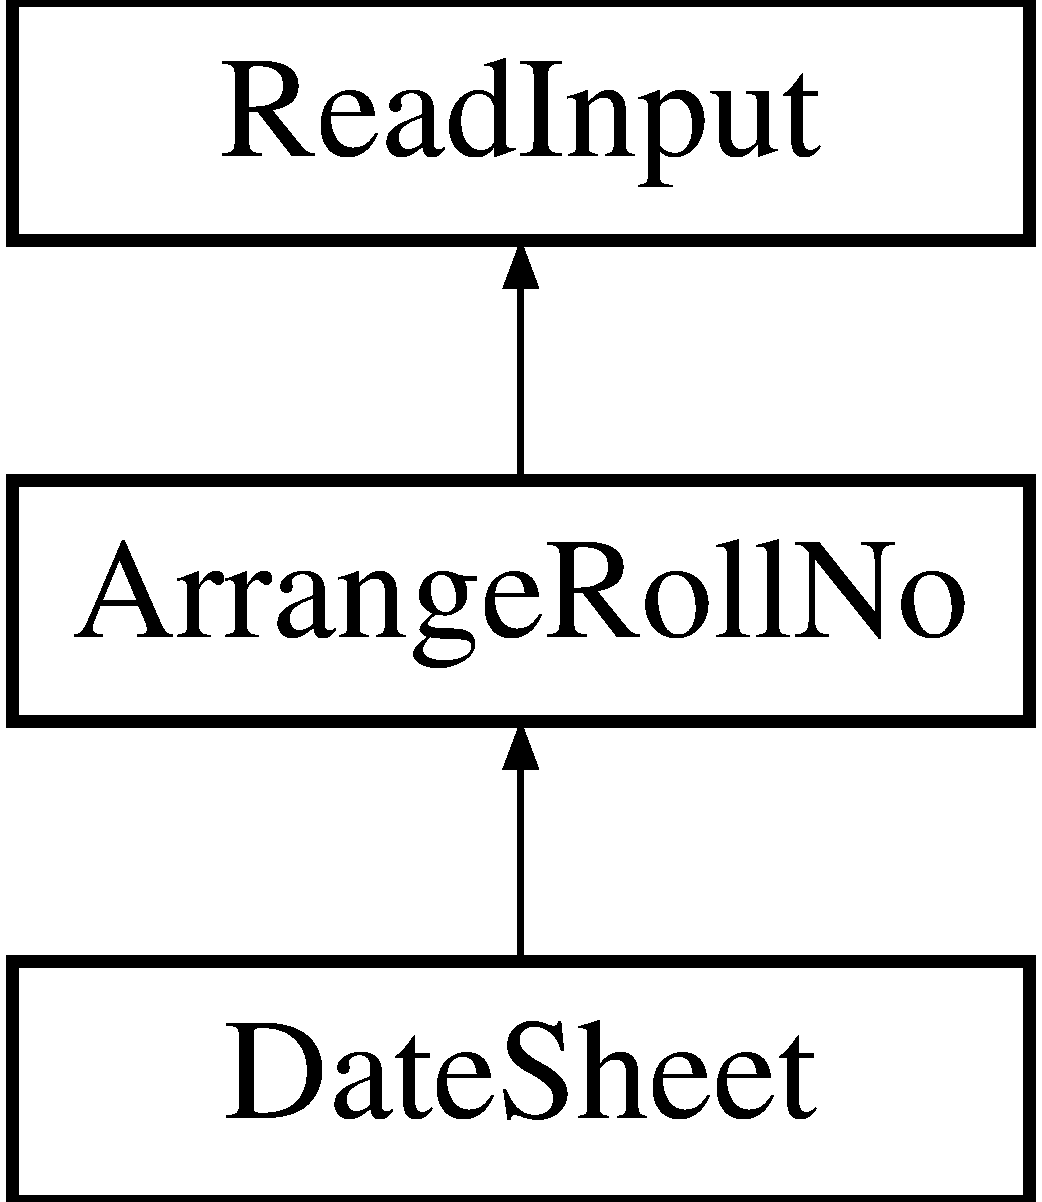
\includegraphics[height=3.000000cm]{classDateSheet}
\end{center}
\end{figure}
\subsection*{Public Member Functions}
\begin{DoxyCompactItemize}
\item 
\hyperlink{classDateSheet_a17a1e5adc9b48e53091b89061ee0a360}{Date\-Sheet} ()
\begin{DoxyCompactList}\small\item\em Constructor. \end{DoxyCompactList}\item 
void \hyperlink{classDateSheet_a8c1bd0daf35e3ea6f962a03fe78cdfa3}{Add\-Roll\-No\-With\-Date\-Sheet} ()
\begin{DoxyCompactList}\small\item\em Adding roll no to with exam subject code in datesheet. \end{DoxyCompactList}\item 
void \hyperlink{classDateSheet_a3f7ea57a0ed85dc6c09f0eda9c30016b}{Write\-Date\-Sheet} (string \hyperlink{classInputDetail_a08069ee622c626c038b821ddcc7427b4}{project\-I\-D})
\item 
void \hyperlink{classDateSheet_af749306c14297b5c93c16f48f551d5bb}{Main} (string p\-I\-D)
\item 
\hyperlink{classDateSheet_af17d25ae4f39caf7b9ea62d73541813b}{$\sim$\-Date\-Sheet} ()
\begin{DoxyCompactList}\small\item\em D\-Estructor. \end{DoxyCompactList}\item 
\hyperlink{classDateSheet_a17a1e5adc9b48e53091b89061ee0a360}{Date\-Sheet} ()
\item 
void \hyperlink{classDateSheet_a0d68cd26658c7dfc37ef512e6ed30528}{Read\-Roll\-No\-Detail} ()
\begin{DoxyCompactList}\small\item\em Reading roll no details filled by user. \end{DoxyCompactList}\item 
void \hyperlink{classDateSheet_ab34e451b5322710f149a1fff5386d852}{Write\-Roll\-No\-Detail} ()
\begin{DoxyCompactList}\small\item\em Writing rol no details into database. \end{DoxyCompactList}\item 
void \hyperlink{classDateSheet_a2eab7d9256cd56064671ac4974846a7a}{Set\-Default\-Value} ()
\begin{DoxyCompactList}\small\item\em Setting default values for i/p field of datesheet. \end{DoxyCompactList}\item 
void \hyperlink{classDateSheet_a3a1721837309480f64f78745b865615f}{Date\-Sheet\-Page} ()
\begin{DoxyCompactList}\small\item\em \hyperlink{classDateSheet}{Date\-Sheet} Page for taking I/\-P from user. \end{DoxyCompactList}\item 
\hyperlink{classDateSheet_af17d25ae4f39caf7b9ea62d73541813b}{$\sim$\-Date\-Sheet} ()
\end{DoxyCompactItemize}
\subsection*{Additional Inherited Members}


\subsection{Detailed Description}
\hyperlink{classDateSheet}{Date\-Sheet} class for reading datesheet detail, class detail and create datesheet.\-out file for seating plan. 

Datesheet class for taking datesheet detail from user.

Include \hyperlink{arrangerollno_8h}{arrangerollno.\-h} header file

include datesheet.\-h

include \hyperlink{inputdetail_8h_source}{inputdetail.\-h} 

Definition at line 27 of file datesheet.\-h.



\subsection{Constructor \& Destructor Documentation}
\hypertarget{classDateSheet_a17a1e5adc9b48e53091b89061ee0a360}{\index{Date\-Sheet@{Date\-Sheet}!Date\-Sheet@{Date\-Sheet}}
\index{Date\-Sheet@{Date\-Sheet}!DateSheet@{Date\-Sheet}}
\subsubsection[{Date\-Sheet}]{\setlength{\rightskip}{0pt plus 5cm}Date\-Sheet\-::\-Date\-Sheet (
\begin{DoxyParamCaption}
{}
\end{DoxyParamCaption}
)}}\label{classDateSheet_a17a1e5adc9b48e53091b89061ee0a360}


Constructor. 

Constructor 

Definition at line 27 of file datesheet.\-cc.

\hypertarget{classDateSheet_af17d25ae4f39caf7b9ea62d73541813b}{\index{Date\-Sheet@{Date\-Sheet}!$\sim$\-Date\-Sheet@{$\sim$\-Date\-Sheet}}
\index{$\sim$\-Date\-Sheet@{$\sim$\-Date\-Sheet}!DateSheet@{Date\-Sheet}}
\subsubsection[{$\sim$\-Date\-Sheet}]{\setlength{\rightskip}{0pt plus 5cm}Date\-Sheet\-::$\sim$\-Date\-Sheet (
\begin{DoxyParamCaption}
{}
\end{DoxyParamCaption}
)}}\label{classDateSheet_af17d25ae4f39caf7b9ea62d73541813b}


D\-Estructor. 

Desructor 

Definition at line 161 of file datesheet.\-cc.

\hypertarget{classDateSheet_a17a1e5adc9b48e53091b89061ee0a360}{\index{Date\-Sheet@{Date\-Sheet}!Date\-Sheet@{Date\-Sheet}}
\index{Date\-Sheet@{Date\-Sheet}!DateSheet@{Date\-Sheet}}
\subsubsection[{Date\-Sheet}]{\setlength{\rightskip}{0pt plus 5cm}Date\-Sheet\-::\-Date\-Sheet (
\begin{DoxyParamCaption}
{}
\end{DoxyParamCaption}
)}}\label{classDateSheet_a17a1e5adc9b48e53091b89061ee0a360}
Constructor \hypertarget{classDateSheet_af17d25ae4f39caf7b9ea62d73541813b}{\index{Date\-Sheet@{Date\-Sheet}!$\sim$\-Date\-Sheet@{$\sim$\-Date\-Sheet}}
\index{$\sim$\-Date\-Sheet@{$\sim$\-Date\-Sheet}!DateSheet@{Date\-Sheet}}
\subsubsection[{$\sim$\-Date\-Sheet}]{\setlength{\rightskip}{0pt plus 5cm}Date\-Sheet\-::$\sim$\-Date\-Sheet (
\begin{DoxyParamCaption}
{}
\end{DoxyParamCaption}
)}}\label{classDateSheet_af17d25ae4f39caf7b9ea62d73541813b}
Destructor 

\subsection{Member Function Documentation}
\hypertarget{classDateSheet_a8c1bd0daf35e3ea6f962a03fe78cdfa3}{\index{Date\-Sheet@{Date\-Sheet}!Add\-Roll\-No\-With\-Date\-Sheet@{Add\-Roll\-No\-With\-Date\-Sheet}}
\index{Add\-Roll\-No\-With\-Date\-Sheet@{Add\-Roll\-No\-With\-Date\-Sheet}!DateSheet@{Date\-Sheet}}
\subsubsection[{Add\-Roll\-No\-With\-Date\-Sheet}]{\setlength{\rightskip}{0pt plus 5cm}void Date\-Sheet\-::\-Add\-Roll\-No\-With\-Date\-Sheet (
\begin{DoxyParamCaption}
{}
\end{DoxyParamCaption}
)}}\label{classDateSheet_a8c1bd0daf35e3ea6f962a03fe78cdfa3}


Adding roll no to with exam subject code in datesheet. 

Adding roll nos with date sheet 

Definition at line 38 of file datesheet.\-cc.

\hypertarget{classDateSheet_a3a1721837309480f64f78745b865615f}{\index{Date\-Sheet@{Date\-Sheet}!Date\-Sheet\-Page@{Date\-Sheet\-Page}}
\index{Date\-Sheet\-Page@{Date\-Sheet\-Page}!DateSheet@{Date\-Sheet}}
\subsubsection[{Date\-Sheet\-Page}]{\setlength{\rightskip}{0pt plus 5cm}void Date\-Sheet\-::\-Date\-Sheet\-Page (
\begin{DoxyParamCaption}
{}
\end{DoxyParamCaption}
)}}\label{classDateSheet_a3a1721837309480f64f78745b865615f}


\hyperlink{classDateSheet}{Date\-Sheet} Page for taking I/\-P from user. 

\hyperlink{classDateSheet}{Date\-Sheet} page for taking I/\-P from user 

Definition at line 183 of file datesheet.\-cc.

\hypertarget{classDateSheet_af749306c14297b5c93c16f48f551d5bb}{\index{Date\-Sheet@{Date\-Sheet}!Main@{Main}}
\index{Main@{Main}!DateSheet@{Date\-Sheet}}
\subsubsection[{Main}]{\setlength{\rightskip}{0pt plus 5cm}void Date\-Sheet\-::\-Main (
\begin{DoxyParamCaption}
\item[{string}]{p\-I\-D}
\end{DoxyParamCaption}
)}}\label{classDateSheet_af749306c14297b5c93c16f48f551d5bb}
Main function to call other functions 

Definition at line 143 of file datesheet.\-cc.

\hypertarget{classDateSheet_a0d68cd26658c7dfc37ef512e6ed30528}{\index{Date\-Sheet@{Date\-Sheet}!Read\-Roll\-No\-Detail@{Read\-Roll\-No\-Detail}}
\index{Read\-Roll\-No\-Detail@{Read\-Roll\-No\-Detail}!DateSheet@{Date\-Sheet}}
\subsubsection[{Read\-Roll\-No\-Detail}]{\setlength{\rightskip}{0pt plus 5cm}void Date\-Sheet\-::\-Read\-Roll\-No\-Detail (
\begin{DoxyParamCaption}
{}
\end{DoxyParamCaption}
)}}\label{classDateSheet_a0d68cd26658c7dfc37ef512e6ed30528}


Reading roll no details filled by user. 

Read\-Roll\-No detail 

Definition at line 45 of file datesheet.\-cc.

\hypertarget{classDateSheet_a2eab7d9256cd56064671ac4974846a7a}{\index{Date\-Sheet@{Date\-Sheet}!Set\-Default\-Value@{Set\-Default\-Value}}
\index{Set\-Default\-Value@{Set\-Default\-Value}!DateSheet@{Date\-Sheet}}
\subsubsection[{Set\-Default\-Value}]{\setlength{\rightskip}{0pt plus 5cm}void Date\-Sheet\-::\-Set\-Default\-Value (
\begin{DoxyParamCaption}
{}
\end{DoxyParamCaption}
)}}\label{classDateSheet_a2eab7d9256cd56064671ac4974846a7a}


Setting default values for i/p field of datesheet. 

Setting dafalut values for datedheet page 

Definition at line 167 of file datesheet.\-cc.

\hypertarget{classDateSheet_a3f7ea57a0ed85dc6c09f0eda9c30016b}{\index{Date\-Sheet@{Date\-Sheet}!Write\-Date\-Sheet@{Write\-Date\-Sheet}}
\index{Write\-Date\-Sheet@{Write\-Date\-Sheet}!DateSheet@{Date\-Sheet}}
\subsubsection[{Write\-Date\-Sheet}]{\setlength{\rightskip}{0pt plus 5cm}void Date\-Sheet\-::\-Write\-Date\-Sheet (
\begin{DoxyParamCaption}
\item[{string}]{project\-I\-D}
\end{DoxyParamCaption}
)}}\label{classDateSheet_a3f7ea57a0ed85dc6c09f0eda9c30016b}
Writing datesheet.\-out file i.\-e. used for seating plan 

Definition at line 99 of file datesheet.\-cc.

\hypertarget{classDateSheet_ab34e451b5322710f149a1fff5386d852}{\index{Date\-Sheet@{Date\-Sheet}!Write\-Roll\-No\-Detail@{Write\-Roll\-No\-Detail}}
\index{Write\-Roll\-No\-Detail@{Write\-Roll\-No\-Detail}!DateSheet@{Date\-Sheet}}
\subsubsection[{Write\-Roll\-No\-Detail}]{\setlength{\rightskip}{0pt plus 5cm}void Date\-Sheet\-::\-Write\-Roll\-No\-Detail (
\begin{DoxyParamCaption}
{}
\end{DoxyParamCaption}
)}}\label{classDateSheet_ab34e451b5322710f149a1fff5386d852}


Writing rol no details into database. 

Write roll no detail into database 

Definition at line 114 of file datesheet.\-cc.



The documentation for this class was generated from the following files\-:\begin{DoxyCompactItemize}
\item 
frontend/src/backend/header/datesheet.\-h\item 
frontend/src/header/datesheet.\-h\item 
frontend/src/backend/datesheet.\-cc\item 
frontend/src/datesheet.\-cc\end{DoxyCompactItemize}

\hypertarget{classExamDetail}{\section{\-Exam\-Detail \-Class \-Reference}
\label{classExamDetail}\index{\-Exam\-Detail@{\-Exam\-Detail}}
}


\hyperlink{classExamDetail}{\-Exam\-Detail} class for getting exam from user.  




{\ttfamily \#include $<$exam.\-h$>$}

\-Inheritance diagram for \-Exam\-Detail\-:\begin{figure}[H]
\begin{center}
\leavevmode
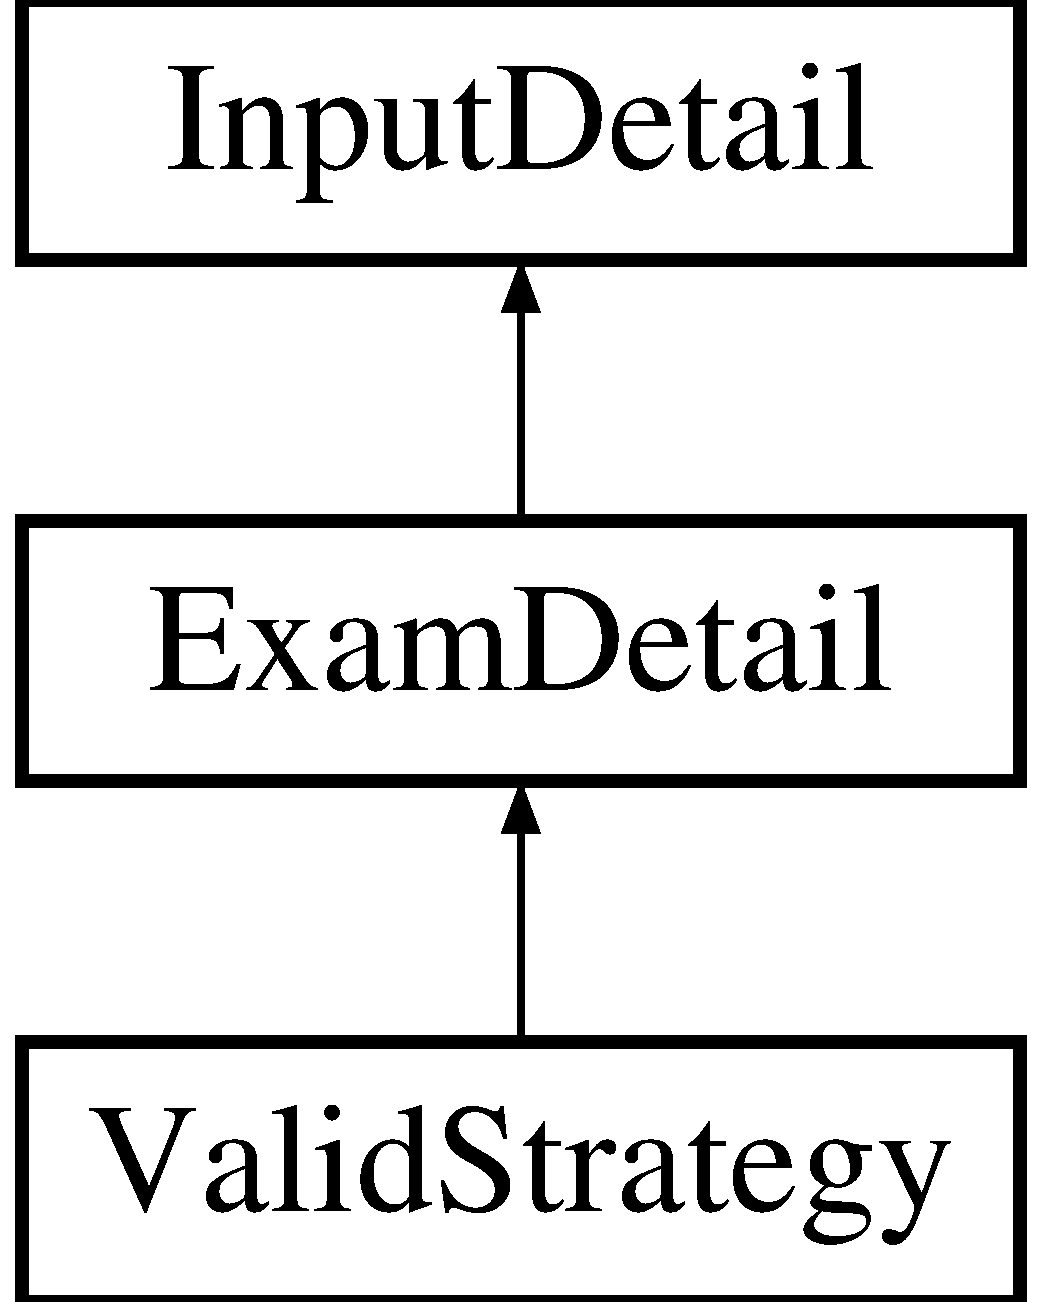
\includegraphics[height=3.000000cm]{classExamDetail}
\end{center}
\end{figure}
\subsection*{\-Public \-Member \-Functions}
\begin{DoxyCompactItemize}
\item 
\hyperlink{classExamDetail_ad555c8a79c821f4e9e75c9b882366991}{\-Exam\-Detail} ()
\begin{DoxyCompactList}\small\item\em \-Constructor. \end{DoxyCompactList}\item 
void \hyperlink{classExamDetail_a460c5736a52aa73ee2627a322d9022f8}{\-Read\-Room\-Detail} ()
\begin{DoxyCompactList}\small\item\em \-Reading room details from previous page. \end{DoxyCompactList}\item 
void \hyperlink{classExamDetail_a51cb1af0e7d6f077aa662b120fd7aec2}{\-Write\-Room\-Detail} ()
\begin{DoxyCompactList}\small\item\em \-After \-Reading, saving details in \hyperlink{classDatabase}{\-Database}. \end{DoxyCompactList}\item 
void \hyperlink{classExamDetail_a3f17d1b2a87cf9530ce2dc5c65244165}{\-Set\-Default\-Value} ()
\begin{DoxyCompactList}\small\item\em \-Setting \-Default values for exam fields if projecy is new or old project has empty detail in database. \end{DoxyCompactList}\item 
void \hyperlink{classExamDetail_aa5bccd1f578e6149ad212206e95d9d57}{\-Exam\-Detail\-Page} ()
\begin{DoxyCompactList}\small\item\em \-Page for taking exam detail. \end{DoxyCompactList}\item 
\hyperlink{classExamDetail_ac613efeb54bd3ddc025b6665e23eb3b0}{$\sim$\-Exam\-Detail} ()
\begin{DoxyCompactList}\small\item\em \-Destructor. \end{DoxyCompactList}\end{DoxyCompactItemize}


\subsection{\-Detailed \-Description}
\hyperlink{classExamDetail}{\-Exam\-Detail} class for getting exam from user. 

\-Include \hyperlink{exam_8h}{exam.\-h}

\-Include \hyperlink{inputdetail_8h_source}{inputdetail.\-h} 

\-Definition at line 29 of file exam.\-h.



\subsection{\-Constructor \& \-Destructor \-Documentation}
\hypertarget{classExamDetail_ad555c8a79c821f4e9e75c9b882366991}{\index{\-Exam\-Detail@{\-Exam\-Detail}!\-Exam\-Detail@{\-Exam\-Detail}}
\index{\-Exam\-Detail@{\-Exam\-Detail}!ExamDetail@{\-Exam\-Detail}}
\subsubsection[{\-Exam\-Detail}]{\setlength{\rightskip}{0pt plus 5cm}{\bf \-Exam\-Detail\-::\-Exam\-Detail} (
\begin{DoxyParamCaption}
{}
\end{DoxyParamCaption}
)}}\label{classExamDetail_ad555c8a79c821f4e9e75c9b882366991}


\-Constructor. 

\-Constroctor 

\-Definition at line 27 of file exam.\-cc.

\hypertarget{classExamDetail_ac613efeb54bd3ddc025b6665e23eb3b0}{\index{\-Exam\-Detail@{\-Exam\-Detail}!$\sim$\-Exam\-Detail@{$\sim$\-Exam\-Detail}}
\index{$\sim$\-Exam\-Detail@{$\sim$\-Exam\-Detail}!ExamDetail@{\-Exam\-Detail}}
\subsubsection[{$\sim$\-Exam\-Detail}]{\setlength{\rightskip}{0pt plus 5cm}{\bf \-Exam\-Detail\-::$\sim$\-Exam\-Detail} (
\begin{DoxyParamCaption}
{}
\end{DoxyParamCaption}
)}}\label{classExamDetail_ac613efeb54bd3ddc025b6665e23eb3b0}


\-Destructor. 

\-Destructor 

\-Definition at line 571 of file exam.\-cc.



\subsection{\-Member \-Function \-Documentation}
\hypertarget{classExamDetail_aa5bccd1f578e6149ad212206e95d9d57}{\index{\-Exam\-Detail@{\-Exam\-Detail}!\-Exam\-Detail\-Page@{\-Exam\-Detail\-Page}}
\index{\-Exam\-Detail\-Page@{\-Exam\-Detail\-Page}!ExamDetail@{\-Exam\-Detail}}
\subsubsection[{\-Exam\-Detail\-Page}]{\setlength{\rightskip}{0pt plus 5cm}void {\bf \-Exam\-Detail\-::\-Exam\-Detail\-Page} (
\begin{DoxyParamCaption}
{}
\end{DoxyParamCaption}
)}}\label{classExamDetail_aa5bccd1f578e6149ad212206e95d9d57}


\-Page for taking exam detail. 

\-Exam \-Detail \-Page 

\-Definition at line 327 of file exam.\-cc.

\hypertarget{classExamDetail_a460c5736a52aa73ee2627a322d9022f8}{\index{\-Exam\-Detail@{\-Exam\-Detail}!\-Read\-Room\-Detail@{\-Read\-Room\-Detail}}
\index{\-Read\-Room\-Detail@{\-Read\-Room\-Detail}!ExamDetail@{\-Exam\-Detail}}
\subsubsection[{\-Read\-Room\-Detail}]{\setlength{\rightskip}{0pt plus 5cm}void {\bf \-Exam\-Detail\-::\-Read\-Room\-Detail} (
\begin{DoxyParamCaption}
{}
\end{DoxyParamCaption}
)}}\label{classExamDetail_a460c5736a52aa73ee2627a322d9022f8}


\-Reading room details from previous page. 

\-Reading room detail 

\-Reimplemented in \hyperlink{classValidStrategy_acf1a8763ec29b441c822a9ab8c80dc4b}{\-Valid\-Strategy}.



\-Definition at line 106 of file exam.\-cc.

\hypertarget{classExamDetail_a3f17d1b2a87cf9530ce2dc5c65244165}{\index{\-Exam\-Detail@{\-Exam\-Detail}!\-Set\-Default\-Value@{\-Set\-Default\-Value}}
\index{\-Set\-Default\-Value@{\-Set\-Default\-Value}!ExamDetail@{\-Exam\-Detail}}
\subsubsection[{\-Set\-Default\-Value}]{\setlength{\rightskip}{0pt plus 5cm}void {\bf \-Exam\-Detail\-::\-Set\-Default\-Value} (
\begin{DoxyParamCaption}
{}
\end{DoxyParamCaption}
)}}\label{classExamDetail_a3f17d1b2a87cf9530ce2dc5c65244165}


\-Setting \-Default values for exam fields if projecy is new or old project has empty detail in database. 

\-Setting default values 

\-Definition at line 48 of file exam.\-cc.

\hypertarget{classExamDetail_a51cb1af0e7d6f077aa662b120fd7aec2}{\index{\-Exam\-Detail@{\-Exam\-Detail}!\-Write\-Room\-Detail@{\-Write\-Room\-Detail}}
\index{\-Write\-Room\-Detail@{\-Write\-Room\-Detail}!ExamDetail@{\-Exam\-Detail}}
\subsubsection[{\-Write\-Room\-Detail}]{\setlength{\rightskip}{0pt plus 5cm}void {\bf \-Exam\-Detail\-::\-Write\-Room\-Detail} (
\begin{DoxyParamCaption}
{}
\end{DoxyParamCaption}
)}}\label{classExamDetail_a51cb1af0e7d6f077aa662b120fd7aec2}


\-After \-Reading, saving details in \hyperlink{classDatabase}{\-Database}. 

\-Writing room details into database 

\-Definition at line 227 of file exam.\-cc.



\-The documentation for this class was generated from the following files\-:\begin{DoxyCompactItemize}
\item 
frontend/src/header/\hyperlink{exam_8h}{exam.\-h}\item 
frontend/src/\hyperlink{exam_8cc}{exam.\-cc}\end{DoxyCompactItemize}

\hypertarget{classExapandRollNo}{\section{Exapand\-Roll\-No Class Reference}
\label{classExapandRollNo}\index{Exapand\-Roll\-No@{Exapand\-Roll\-No}}
}
Inheritance diagram for Exapand\-Roll\-No\-:\begin{figure}[H]
\begin{center}
\leavevmode
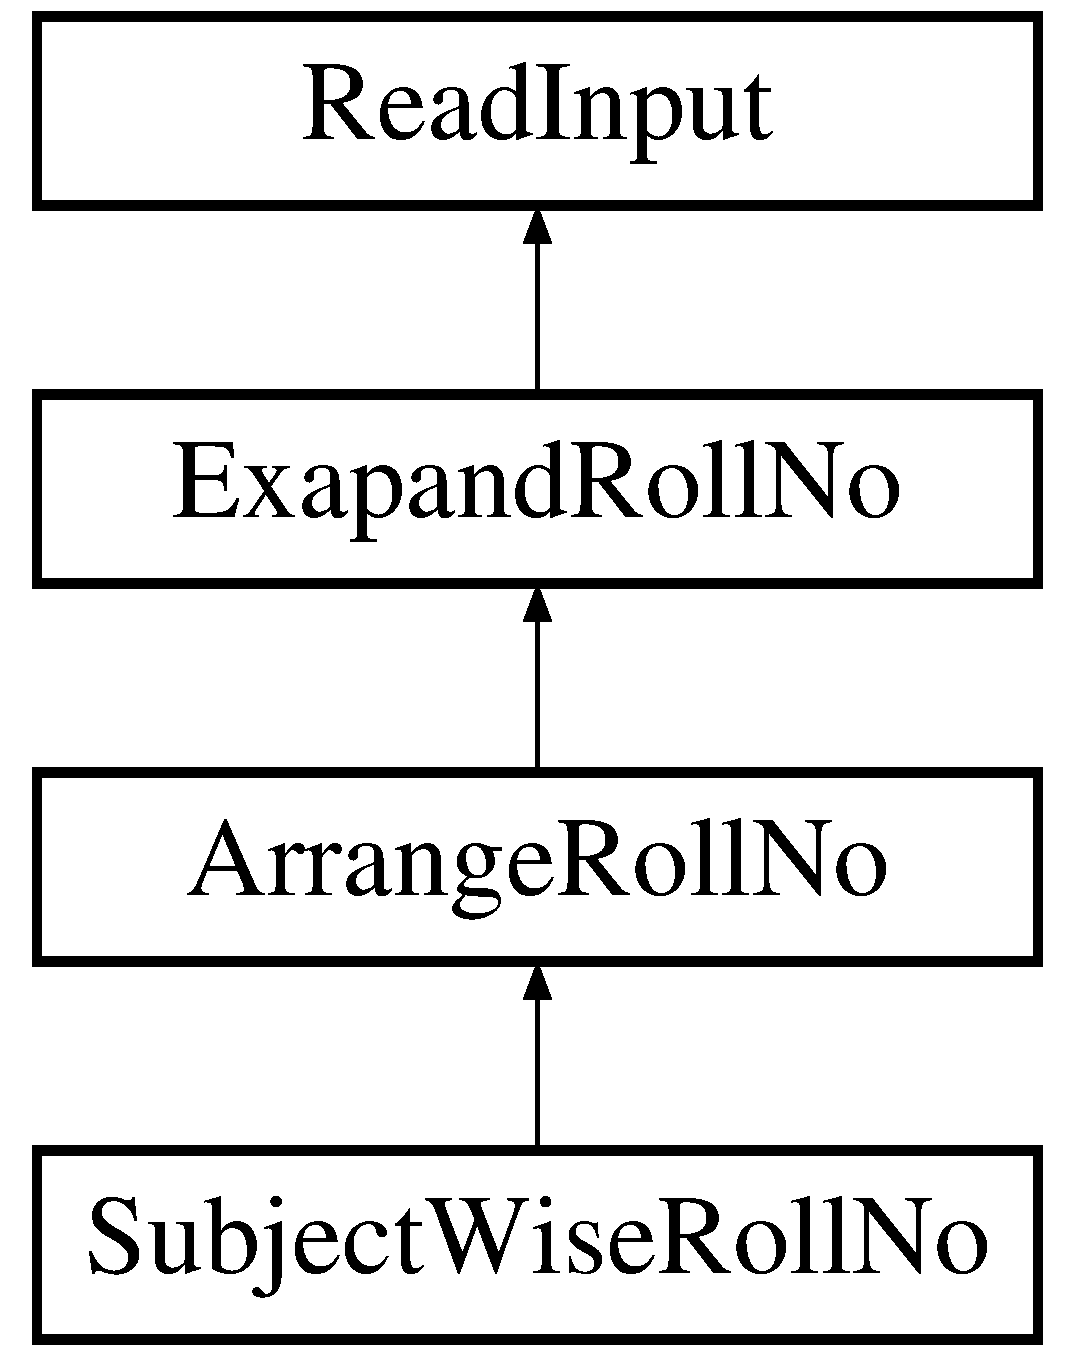
\includegraphics[height=4.000000cm]{classExapandRollNo}
\end{center}
\end{figure}
\subsection*{Public Member Functions}
\begin{DoxyCompactItemize}
\item 
\hypertarget{classExapandRollNo_a19a299d6ebbff3af32fdee08fcc164ee}{void {\bfseries expand\-Input} ()}\label{classExapandRollNo_a19a299d6ebbff3af32fdee08fcc164ee}

\item 
\hypertarget{classExapandRollNo_ad1a2a298aa0834a6da672e152cd4e24f}{void {\bfseries add\-Seperator} ()}\label{classExapandRollNo_ad1a2a298aa0834a6da672e152cd4e24f}

\item 
\hypertarget{classExapandRollNo_a9125b4dc6bbdb81dc4007cec1e86a7e9}{void {\bfseries expand\-Roll\-No} ()}\label{classExapandRollNo_a9125b4dc6bbdb81dc4007cec1e86a7e9}

\item 
\hypertarget{classExapandRollNo_a69ff3dc919a8b297b46926839184b349}{{\footnotesize template$<$typename Out\-Iter $>$ }\\bool {\bfseries expand\-Roll\-Number\-List} (istream \&is, Out\-Iter out)}\label{classExapandRollNo_a69ff3dc919a8b297b46926839184b349}

\item 
\hypertarget{classExapandRollNo_a3b767bfce279771a398abaa725753e33}{void {\bfseries remove\-Zero} ()}\label{classExapandRollNo_a3b767bfce279771a398abaa725753e33}

\item 
\hypertarget{classExapandRollNo_ae11d041a516d6fce629364d6e6796955}{void {\bfseries show\-Expand\-Roll\-No} ()}\label{classExapandRollNo_ae11d041a516d6fce629364d6e6796955}

\item 
\hypertarget{classExapandRollNo_afbfccde139eb71155e0b0fce02962d1c}{void {\bfseries Main} ()}\label{classExapandRollNo_afbfccde139eb71155e0b0fce02962d1c}

\end{DoxyCompactItemize}
\subsection*{Protected Attributes}
\begin{DoxyCompactItemize}
\item 
\hypertarget{classExapandRollNo_ae27a8647cfc7f93a5ba2fbfef8afa5c8}{int {\bfseries roll\-\_\-no} \mbox{[}M\-I\-N\-\_\-\-S\-I\-Z\-E\mbox{]}\mbox{[}M\-A\-X\-\_\-\-S\-I\-Z\-E\mbox{]}\mbox{[}M\-A\-X\-\_\-\-S\-I\-Z\-E\mbox{]}}\label{classExapandRollNo_ae27a8647cfc7f93a5ba2fbfef8afa5c8}

\item 
\hypertarget{classExapandRollNo_a892479a25a021a95e9c4b38ed30208a5}{int {\bfseries roll\-\_\-size} \mbox{[}M\-I\-N\-\_\-\-S\-I\-Z\-E\mbox{]}\mbox{[}M\-I\-N\-\_\-\-S\-I\-Z\-E\mbox{]}}\label{classExapandRollNo_a892479a25a021a95e9c4b38ed30208a5}

\item 
\hypertarget{classExapandRollNo_ac3526c93e25b52ab118f66150c980dbd}{int {\bfseries not\-\_\-roll\-\_\-no} \mbox{[}M\-I\-N\-\_\-\-S\-I\-Z\-E\mbox{]}\mbox{[}M\-A\-X\-\_\-\-S\-I\-Z\-E\mbox{]}\mbox{[}M\-A\-X\-\_\-\-S\-I\-Z\-E\mbox{]}}\label{classExapandRollNo_ac3526c93e25b52ab118f66150c980dbd}

\item 
\hypertarget{classExapandRollNo_a809856dbd610c81509f2fdf2cc11e57f}{int {\bfseries not\-\_\-roll\-\_\-size} \mbox{[}M\-I\-N\-\_\-\-S\-I\-Z\-E\mbox{]}\mbox{[}M\-I\-N\-\_\-\-S\-I\-Z\-E\mbox{]}}\label{classExapandRollNo_a809856dbd610c81509f2fdf2cc11e57f}

\end{DoxyCompactItemize}


The documentation for this class was generated from the following files\-:\begin{DoxyCompactItemize}
\item 
expand-\/rollno.\-h\item 
expand-\/rollno.\-cc\end{DoxyCompactItemize}

\hypertarget{classExpandRollNo}{\section{\-Expand\-Roll\-No \-Class \-Reference}
\label{classExpandRollNo}\index{\-Expand\-Roll\-No@{\-Expand\-Roll\-No}}
}
\-Inheritance diagram for \-Expand\-Roll\-No\-:\begin{figure}[H]
\begin{center}
\leavevmode
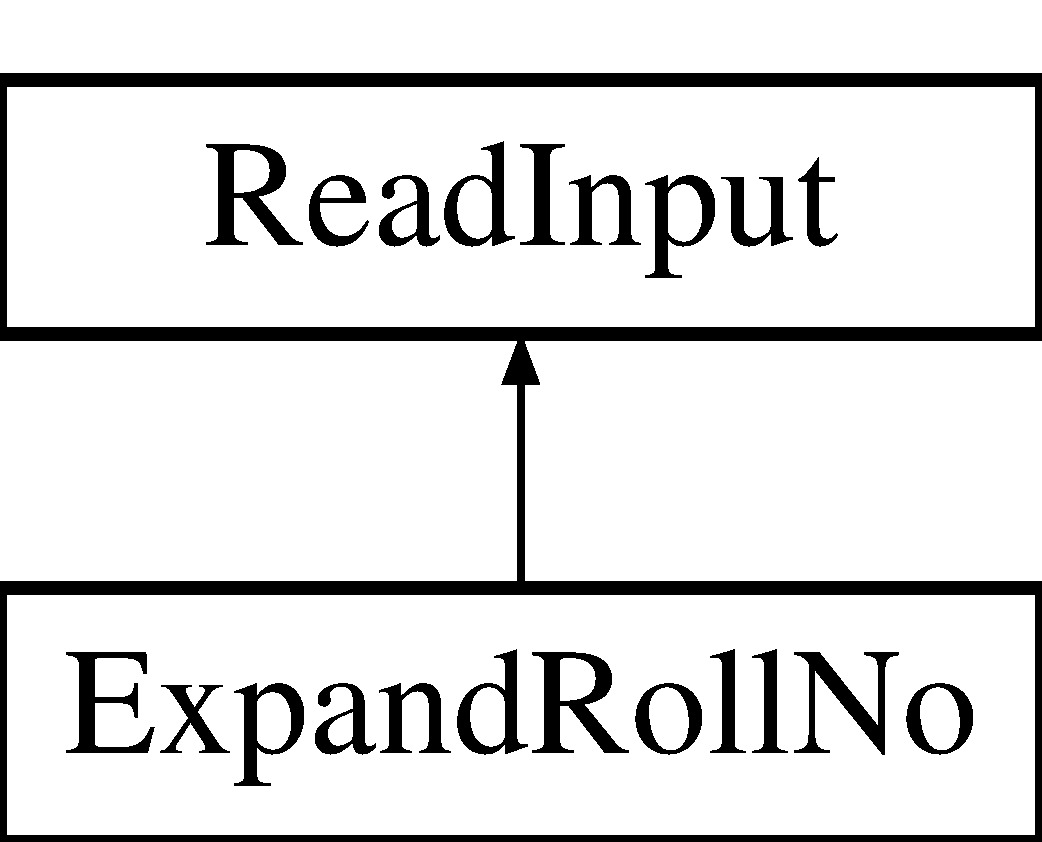
\includegraphics[height=2.000000cm]{classExpandRollNo}
\end{center}
\end{figure}
\subsection*{\-Public \-Member \-Functions}
\begin{DoxyCompactItemize}
\item 
\hyperlink{classExpandRollNo_a60e3a3d50ebe826b6d5c3304757812ca}{\-Expand\-Roll\-No} ()
\item 
{\footnotesize template$<$typename Out\-Iter $>$ }\\bool \hyperlink{classExpandRollNo_afcb476d9d9f1fdabd456f3ec84b14184}{\-Expand\-Roll\-No\-List} (istream \&is, \-Out\-Iter out)
\begin{DoxyCompactList}\small\item\em \-Templete for expanding roll nos. \end{DoxyCompactList}\item 
void \hyperlink{classExpandRollNo_a4917831a98da9aa068b2589945b46065}{\-Expand\-Roll\-Nos} (string \hyperlink{classReadInput_a3ad470a25b3e0a29466bf4ff1f7d8e81}{project\-I\-D})
\begin{DoxyCompactList}\small\item\em \-Expanding \-Roll nos. \end{DoxyCompactList}\item 
void \hyperlink{classExpandRollNo_af95bc4c35354c225bdfff5fae7f6b845}{\-Write\-Expand\-Roll\-No} (string \hyperlink{classReadInput_a3ad470a25b3e0a29466bf4ff1f7d8e81}{project\-I\-D})
\begin{DoxyCompactList}\small\item\em \-Write expanded roll nos into file. \end{DoxyCompactList}\item 
\hyperlink{classExpandRollNo_acf3cb7b789bd49a79672cb93dac2ed7c}{$\sim$\-Expand\-Roll\-No} ()
\begin{DoxyCompactList}\small\item\em \-Destructor. \end{DoxyCompactList}\end{DoxyCompactItemize}
\subsection*{\-Protected \-Attributes}
\begin{DoxyCompactItemize}
\item 
\hypertarget{classExpandRollNo_a048403e926bacac445f692538e5e3b81}{\-I\-N\-T\-\_\-\-V\-E\-C {\bfseries roll\-No\-Size}}\label{classExpandRollNo_a048403e926bacac445f692538e5e3b81}

\item 
\hypertarget{classExpandRollNo_af998ac9fe5669a5d2a379faba52a57cc}{\-I\-N\-T\-\_\-\-V\-E\-C {\bfseries not\-Included\-R\-No\-Size}}\label{classExpandRollNo_af998ac9fe5669a5d2a379faba52a57cc}

\end{DoxyCompactItemize}


\subsection{\-Detailed \-Description}


\-Definition at line 27 of file expandrollno.\-h.



\subsection{\-Constructor \& \-Destructor \-Documentation}
\hypertarget{classExpandRollNo_a60e3a3d50ebe826b6d5c3304757812ca}{\index{\-Expand\-Roll\-No@{\-Expand\-Roll\-No}!\-Expand\-Roll\-No@{\-Expand\-Roll\-No}}
\index{\-Expand\-Roll\-No@{\-Expand\-Roll\-No}!ExpandRollNo@{\-Expand\-Roll\-No}}
\subsubsection[{\-Expand\-Roll\-No}]{\setlength{\rightskip}{0pt plus 5cm}{\bf \-Expand\-Roll\-No\-::\-Expand\-Roll\-No} (
\begin{DoxyParamCaption}
{}
\end{DoxyParamCaption}
)}}\label{classExpandRollNo_a60e3a3d50ebe826b6d5c3304757812ca}
\-Constructor

include \hyperlink{expandrollno_8h}{expandrollno.\-h} 

\-Definition at line 22 of file expandrollno.\-cc.

\hypertarget{classExpandRollNo_acf3cb7b789bd49a79672cb93dac2ed7c}{\index{\-Expand\-Roll\-No@{\-Expand\-Roll\-No}!$\sim$\-Expand\-Roll\-No@{$\sim$\-Expand\-Roll\-No}}
\index{$\sim$\-Expand\-Roll\-No@{$\sim$\-Expand\-Roll\-No}!ExpandRollNo@{\-Expand\-Roll\-No}}
\subsubsection[{$\sim$\-Expand\-Roll\-No}]{\setlength{\rightskip}{0pt plus 5cm}{\bf \-Expand\-Roll\-No\-::$\sim$\-Expand\-Roll\-No} (
\begin{DoxyParamCaption}
{}
\end{DoxyParamCaption}
)}}\label{classExpandRollNo_acf3cb7b789bd49a79672cb93dac2ed7c}


\-Destructor. 

\-Destructor 

\-Definition at line 195 of file expandrollno.\-cc.



\subsection{\-Member \-Function \-Documentation}
\hypertarget{classExpandRollNo_afcb476d9d9f1fdabd456f3ec84b14184}{\index{\-Expand\-Roll\-No@{\-Expand\-Roll\-No}!\-Expand\-Roll\-No\-List@{\-Expand\-Roll\-No\-List}}
\index{\-Expand\-Roll\-No\-List@{\-Expand\-Roll\-No\-List}!ExpandRollNo@{\-Expand\-Roll\-No}}
\subsubsection[{\-Expand\-Roll\-No\-List}]{\setlength{\rightskip}{0pt plus 5cm}template$<$typename Out\-Iter $>$ bool {\bf \-Expand\-Roll\-No\-::\-Expand\-Roll\-No\-List} (
\begin{DoxyParamCaption}
\item[{istream \&}]{is, }
\item[{\-Out\-Iter}]{out}
\end{DoxyParamCaption}
)}}\label{classExpandRollNo_afcb476d9d9f1fdabd456f3ec84b14184}


\-Templete for expanding roll nos. 

\-Template for expanding roll no 

\-Definition at line 94 of file expandrollno.\-cc.

\hypertarget{classExpandRollNo_a4917831a98da9aa068b2589945b46065}{\index{\-Expand\-Roll\-No@{\-Expand\-Roll\-No}!\-Expand\-Roll\-Nos@{\-Expand\-Roll\-Nos}}
\index{\-Expand\-Roll\-Nos@{\-Expand\-Roll\-Nos}!ExpandRollNo@{\-Expand\-Roll\-No}}
\subsubsection[{\-Expand\-Roll\-Nos}]{\setlength{\rightskip}{0pt plus 5cm}void {\bf \-Expand\-Roll\-No\-::\-Expand\-Roll\-Nos} (
\begin{DoxyParamCaption}
\item[{string}]{project\-I\-D}
\end{DoxyParamCaption}
)}}\label{classExpandRollNo_a4917831a98da9aa068b2589945b46065}


\-Expanding \-Roll nos. 

\-For expanding roll no and calling \-Expand\-Roll\-No\-List templete


\begin{DoxyParams}{\-Parameters}
{\em project\-I\-D} & \-Project \-I\-D of user's project \\
\hline
\end{DoxyParams}


\-Definition at line 34 of file expandrollno.\-cc.

\hypertarget{classExpandRollNo_af95bc4c35354c225bdfff5fae7f6b845}{\index{\-Expand\-Roll\-No@{\-Expand\-Roll\-No}!\-Write\-Expand\-Roll\-No@{\-Write\-Expand\-Roll\-No}}
\index{\-Write\-Expand\-Roll\-No@{\-Write\-Expand\-Roll\-No}!ExpandRollNo@{\-Expand\-Roll\-No}}
\subsubsection[{\-Write\-Expand\-Roll\-No}]{\setlength{\rightskip}{0pt plus 5cm}void {\bf \-Expand\-Roll\-No\-::\-Write\-Expand\-Roll\-No} (
\begin{DoxyParamCaption}
\item[{string}]{project\-I\-D}
\end{DoxyParamCaption}
)}}\label{classExpandRollNo_af95bc4c35354c225bdfff5fae7f6b845}


\-Write expanded roll nos into file. 

\-Write expanded roll no's in file


\begin{DoxyParams}{\-Parameters}
{\em project\-I\-D} & \-Project \-I\-D of user's project \\
\hline
\end{DoxyParams}


\-Definition at line 149 of file expandrollno.\-cc.



\-The documentation for this class was generated from the following files\-:\begin{DoxyCompactItemize}
\item 
frontend/src/backend/header/\hyperlink{expandrollno_8h}{expandrollno.\-h}\item 
frontend/src/backend/\hyperlink{expandrollno_8cc}{expandrollno.\-cc}\end{DoxyCompactItemize}

\hypertarget{classInputDetail}{\section{Input\-Detail Class Reference}
\label{classInputDetail}\index{Input\-Detail@{Input\-Detail}}
}


For declaring common variables and functions also used as base class.  




{\ttfamily \#include $<$input\-\_\-detail.\-h$>$}

Inheritance diagram for Input\-Detail\-:\begin{figure}[H]
\begin{center}
\leavevmode
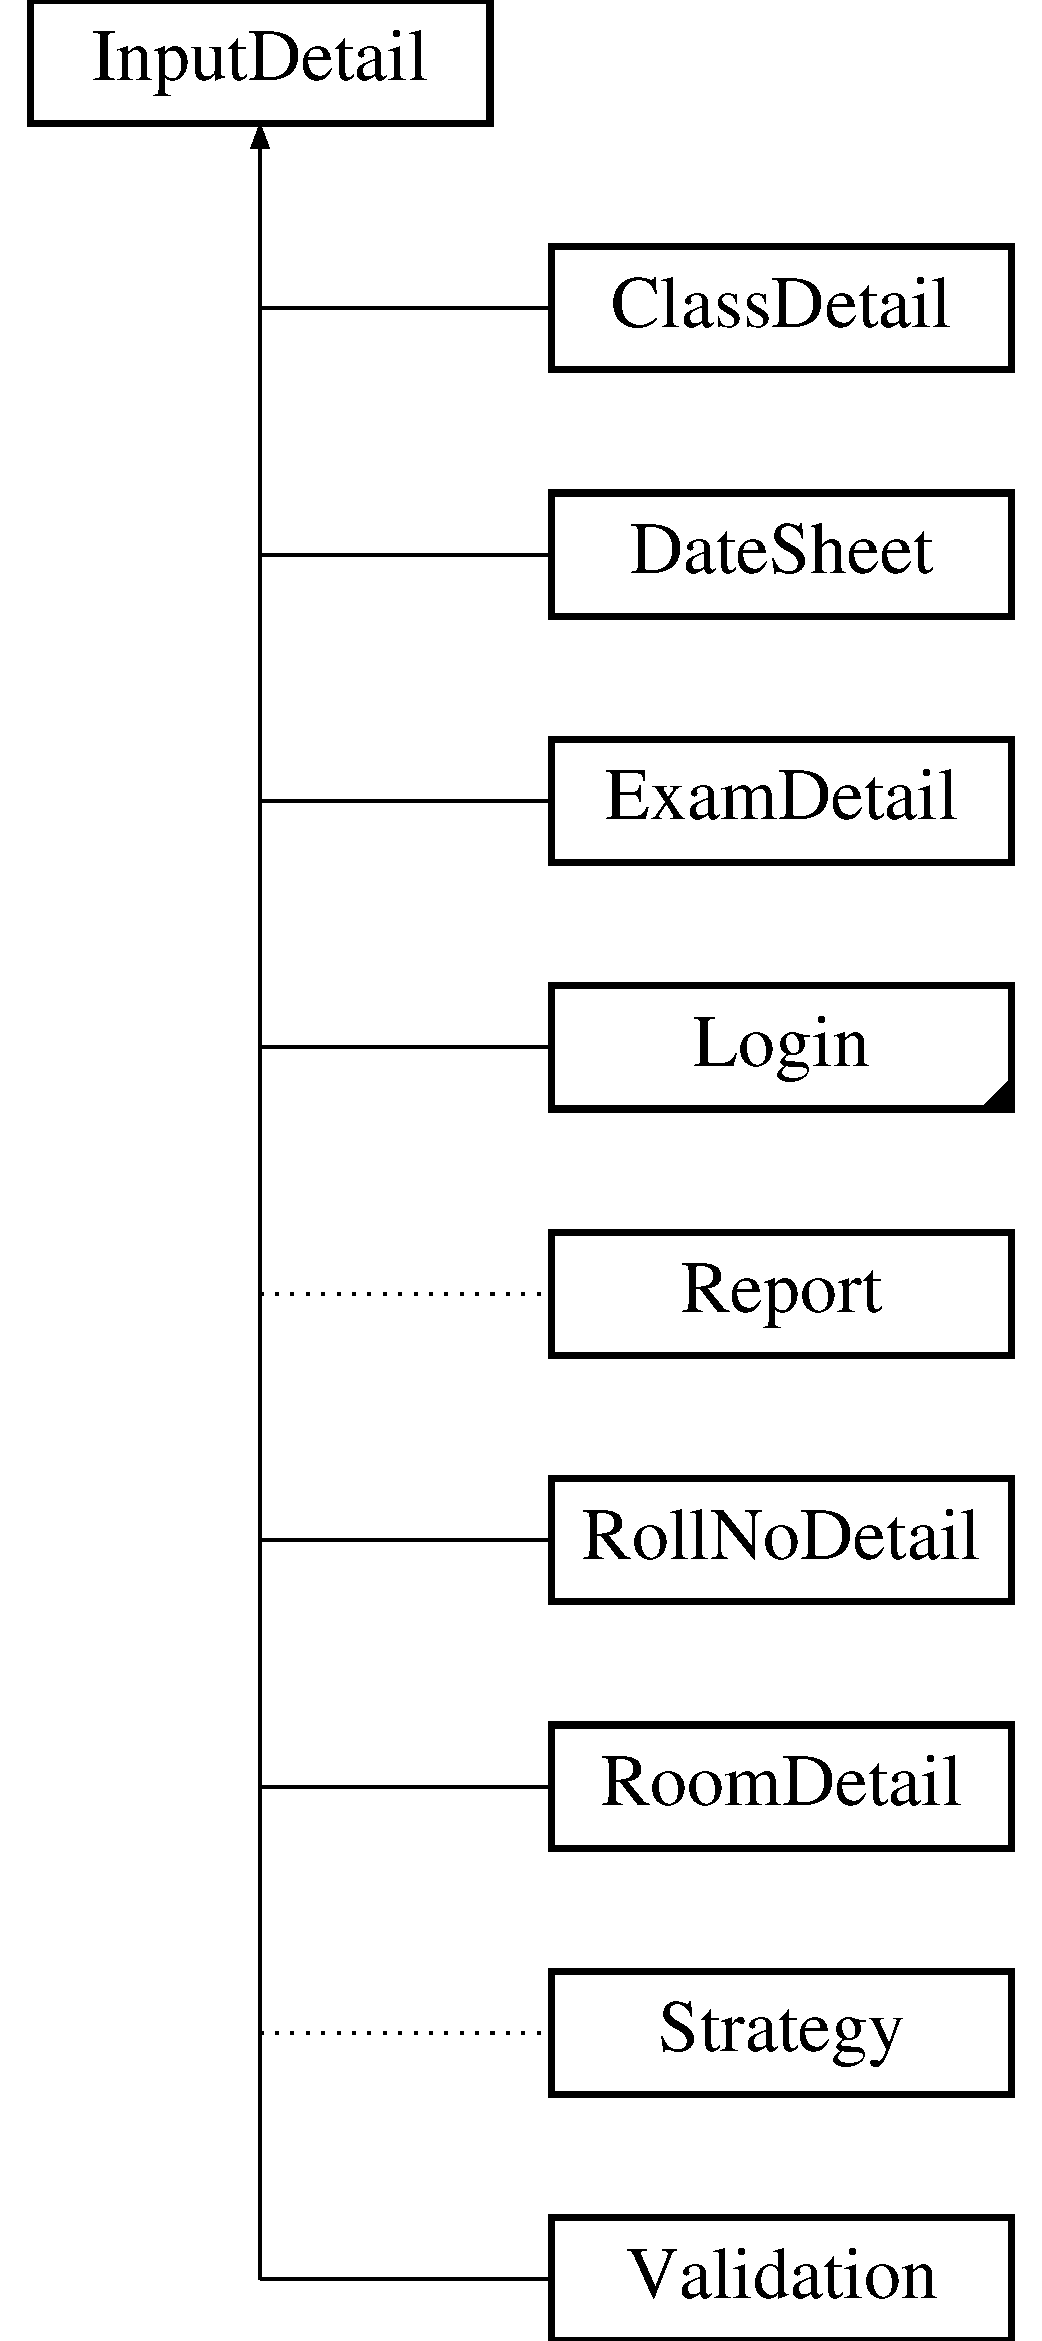
\includegraphics[height=3.000000cm]{classInputDetail}
\end{center}
\end{figure}
\subsection*{Public Member Functions}
\begin{DoxyCompactItemize}
\item 
\hyperlink{classInputDetail_ab53655b14d922eb32b5d5d06c702e497}{Input\-Detail} ()
\begin{DoxyCompactList}\small\item\em Constructor. \end{DoxyCompactList}\item 
string \hyperlink{classInputDetail_ad0a78d7c864bcccf7813a526d59573be}{Int\-To\-String} (int value)
\begin{DoxyCompactList}\small\item\em Converting integer to string. \end{DoxyCompactList}\item 
int \hyperlink{classInputDetail_aaf532dd61f0aee82b116fef2da8e821f}{String\-To\-Int} (string value)
\begin{DoxyCompactList}\small\item\em Converting String to Int. \end{DoxyCompactList}\item 
string \hyperlink{classInputDetail_a509ee6dd2de52e87cb764d0b0cceb05a}{File\-Name} (string file, string project\-I\-D, int file\-Type)
\begin{DoxyCompactList}\small\item\em For creating filename w.\-r.\-t to project\-I\-D. \end{DoxyCompactList}\item 
\hypertarget{classInputDetail_a0dbdaef0be3dc072999e4ae06f5e4e36}{\hyperlink{classInputDetail_a0dbdaef0be3dc072999e4ae06f5e4e36}{$\sim$\-Input\-Detail} ()}\label{classInputDetail_a0dbdaef0be3dc072999e4ae06f5e4e36}

\begin{DoxyCompactList}\small\item\em Destructor. \end{DoxyCompactList}\end{DoxyCompactItemize}
\subsection*{Public Attributes}
\begin{DoxyCompactItemize}
\item 
\hyperlink{classDatabase}{Database} \hyperlink{classInputDetail_ac388f27ccea9830c3c27f68d7134e061}{db}
\item 
\hyperlink{classReadInputField}{Read\-Input\-Field} \hyperlink{classInputDetail_ac0cc70b017ef94fb55acb46fc44f0df5}{read\-Field}
\end{DoxyCompactItemize}
\subsection*{Protected Attributes}
\begin{DoxyCompactItemize}
\item 
\hypertarget{classInputDetail_a2e9226db1b744de4bf406398f48cf962}{int {\bfseries i}}\label{classInputDetail_a2e9226db1b744de4bf406398f48cf962}

\item 
\hypertarget{classInputDetail_af124a26cb4e4f86d0d9eb68200ee500b}{int {\bfseries j}}\label{classInputDetail_af124a26cb4e4f86d0d9eb68200ee500b}

\item 
\hypertarget{classInputDetail_a1bb6b8bff3d5fc6d5c998e4c451035bc}{int {\bfseries k}}\label{classInputDetail_a1bb6b8bff3d5fc6d5c998e4c451035bc}

\item 
int \hyperlink{classInputDetail_a3a950727518c2f6ed3c068125a037b9e}{l}
\item 
stringstream \hyperlink{classInputDetail_a5284736b5fd3db0251cfeab7c581c0bd}{ss}
\item 
\hypertarget{classInputDetail_abacd5d7ee7ebd7e9f36bbf3fefd13a5d}{string {\bfseries temp}}\label{classInputDetail_abacd5d7ee7ebd7e9f36bbf3fefd13a5d}

\item 
string \hyperlink{classInputDetail_aa5659e496977cc83f743725f6aaf2d6a}{temp1}
\item 
\hypertarget{classInputDetail_a08069ee622c626c038b821ddcc7427b4}{string {\bfseries project\-I\-D}}\label{classInputDetail_a08069ee622c626c038b821ddcc7427b4}

\item 
\hypertarget{classInputDetail_ad3f1db4fddbe0d4efbf1d5bc74d52257}{string {\bfseries email\-I\-D}}\label{classInputDetail_ad3f1db4fddbe0d4efbf1d5bc74d52257}

\item 
string \hyperlink{classInputDetail_a4a7fb27e52bed0f40de143634f2c486b}{file\-Name}
\item 
string \hyperlink{classInputDetail_a79d8a59940f25f4d2089e241c71a4279}{where}
\item 
string \hyperlink{classInputDetail_a1abb16cd695678c3fa05e3c812823fee}{msg}
\item 
S\-T\-R\-I\-N\-G\-\_\-\-V\-E\-C \hyperlink{classInputDetail_abee6a659eb2e34b260aaf8b05d6003b4}{vec\-Temp}
\item 
S\-T\-R\-I\-N\-G\-\_\-\-V\-E\-C \hyperlink{classInputDetail_ae8ccc2e838c6d5a93ea544370dc1f272}{old\-Project}
\item 
S\-T\-R\-I\-N\-G\-\_\-\-V\-E\-C \hyperlink{classInputDetail_ab09ed4176090a72237531cedf00afb41}{split\-String}
\item 
ifstream \hyperlink{classInputDetail_a4c62c1934fbfcdcc8e2afaee44a87c15}{in\-File}
\item 
ofstream \hyperlink{classInputDetail_a2b8484cfbfee98ae69e8476f8fd40000}{out\-File}
\item 
string \hyperlink{classInputDetail_a1f276e4df260009d465032ec64f3a543}{session\-I\-D}
\end{DoxyCompactItemize}


\subsection{Detailed Description}
For declaring common variables and functions also used as base class. 

Definition at line 36 of file input\-\_\-detail.\-h.



\subsection{Constructor \& Destructor Documentation}
\hypertarget{classInputDetail_ab53655b14d922eb32b5d5d06c702e497}{\index{Input\-Detail@{Input\-Detail}!Input\-Detail@{Input\-Detail}}
\index{Input\-Detail@{Input\-Detail}!InputDetail@{Input\-Detail}}
\subsubsection[{Input\-Detail}]{\setlength{\rightskip}{0pt plus 5cm}Input\-Detail\-::\-Input\-Detail (
\begin{DoxyParamCaption}
{}
\end{DoxyParamCaption}
)}}\label{classInputDetail_ab53655b14d922eb32b5d5d06c702e497}


Constructor. 

$<$ Shortname for namespace 

Definition at line 23 of file input\-\_\-detail.\-cc.



\subsection{Member Function Documentation}
\hypertarget{classInputDetail_a509ee6dd2de52e87cb764d0b0cceb05a}{\index{Input\-Detail@{Input\-Detail}!File\-Name@{File\-Name}}
\index{File\-Name@{File\-Name}!InputDetail@{Input\-Detail}}
\subsubsection[{File\-Name}]{\setlength{\rightskip}{0pt plus 5cm}string Input\-Detail\-::\-File\-Name (
\begin{DoxyParamCaption}
\item[{string}]{file, }
\item[{string}]{project\-I\-D, }
\item[{int}]{file\-Type}
\end{DoxyParamCaption}
)}}\label{classInputDetail_a509ee6dd2de52e87cb764d0b0cceb05a}


For creating filename w.\-r.\-t to project\-I\-D. 


\begin{DoxyParams}{Parameters}
{\em project\-I\-D} & Unique I\-D i.\-e. used to read file of user \\
\hline
{\em file} & I/\-O file Name \\
\hline
{\em file\-Type} & For defining file type i.\-e I/\-P or O/\-P file. If file\-Type == 1, Input file If file\-Type == 0(else), Output File\\
\hline
\end{DoxyParams}
\begin{DoxyReturn}{Returns}
file\-Name This function will return file name with project I\-D 
\end{DoxyReturn}


Definition at line 82 of file input\-\_\-detail.\-cc.

\hypertarget{classInputDetail_ad0a78d7c864bcccf7813a526d59573be}{\index{Input\-Detail@{Input\-Detail}!Int\-To\-String@{Int\-To\-String}}
\index{Int\-To\-String@{Int\-To\-String}!InputDetail@{Input\-Detail}}
\subsubsection[{Int\-To\-String}]{\setlength{\rightskip}{0pt plus 5cm}string Input\-Detail\-::\-Int\-To\-String (
\begin{DoxyParamCaption}
\item[{int}]{value}
\end{DoxyParamCaption}
)}}\label{classInputDetail_ad0a78d7c864bcccf7813a526d59573be}


Converting integer to string. 


\begin{DoxyParams}{Parameters}
{\em value} & Value to be converted into string \\
\hline
\end{DoxyParams}


Definition at line 35 of file input\-\_\-detail.\-cc.

\hypertarget{classInputDetail_aaf532dd61f0aee82b116fef2da8e821f}{\index{Input\-Detail@{Input\-Detail}!String\-To\-Int@{String\-To\-Int}}
\index{String\-To\-Int@{String\-To\-Int}!InputDetail@{Input\-Detail}}
\subsubsection[{String\-To\-Int}]{\setlength{\rightskip}{0pt plus 5cm}int Input\-Detail\-::\-String\-To\-Int (
\begin{DoxyParamCaption}
\item[{string}]{value}
\end{DoxyParamCaption}
)}}\label{classInputDetail_aaf532dd61f0aee82b116fef2da8e821f}


Converting String to Int. 


\begin{DoxyParams}{Parameters}
{\em value} & String value to be converted into int \\
\hline
\end{DoxyParams}


Definition at line 47 of file input\-\_\-detail.\-cc.



\subsection{Member Data Documentation}
\hypertarget{classInputDetail_ac388f27ccea9830c3c27f68d7134e061}{\index{Input\-Detail@{Input\-Detail}!db@{db}}
\index{db@{db}!InputDetail@{Input\-Detail}}
\subsubsection[{db}]{\setlength{\rightskip}{0pt plus 5cm}{\bf Database} Input\-Detail\-::db}}\label{classInputDetail_ac388f27ccea9830c3c27f68d7134e061}
Data\-Base class's object 

Definition at line 67 of file input\-\_\-detail.\-h.

\hypertarget{classInputDetail_a4a7fb27e52bed0f40de143634f2c486b}{\index{Input\-Detail@{Input\-Detail}!file\-Name@{file\-Name}}
\index{file\-Name@{file\-Name}!InputDetail@{Input\-Detail}}
\subsubsection[{file\-Name}]{\setlength{\rightskip}{0pt plus 5cm}string Input\-Detail\-::file\-Name\hspace{0.3cm}{\ttfamily [protected]}}}\label{classInputDetail_a4a7fb27e52bed0f40de143634f2c486b}
File name for opening file 

Definition at line 49 of file input\-\_\-detail.\-h.

\hypertarget{classInputDetail_a4c62c1934fbfcdcc8e2afaee44a87c15}{\index{Input\-Detail@{Input\-Detail}!in\-File@{in\-File}}
\index{in\-File@{in\-File}!InputDetail@{Input\-Detail}}
\subsubsection[{in\-File}]{\setlength{\rightskip}{0pt plus 5cm}ifstream Input\-Detail\-::in\-File\hspace{0.3cm}{\ttfamily [protected]}}}\label{classInputDetail_a4c62c1934fbfcdcc8e2afaee44a87c15}
For Reading file 

Definition at line 61 of file input\-\_\-detail.\-h.

\hypertarget{classInputDetail_a3a950727518c2f6ed3c068125a037b9e}{\index{Input\-Detail@{Input\-Detail}!l@{l}}
\index{l@{l}!InputDetail@{Input\-Detail}}
\subsubsection[{l}]{\setlength{\rightskip}{0pt plus 5cm}int Input\-Detail\-::l\hspace{0.3cm}{\ttfamily [protected]}}}\label{classInputDetail_a3a950727518c2f6ed3c068125a037b9e}
Looping Variables 

Definition at line 41 of file input\-\_\-detail.\-h.

\hypertarget{classInputDetail_a1abb16cd695678c3fa05e3c812823fee}{\index{Input\-Detail@{Input\-Detail}!msg@{msg}}
\index{msg@{msg}!InputDetail@{Input\-Detail}}
\subsubsection[{msg}]{\setlength{\rightskip}{0pt plus 5cm}string Input\-Detail\-::msg\hspace{0.3cm}{\ttfamily [protected]}}}\label{classInputDetail_a1abb16cd695678c3fa05e3c812823fee}
For Displaying error message 

Definition at line 49 of file input\-\_\-detail.\-h.

\hypertarget{classInputDetail_ae8ccc2e838c6d5a93ea544370dc1f272}{\index{Input\-Detail@{Input\-Detail}!old\-Project@{old\-Project}}
\index{old\-Project@{old\-Project}!InputDetail@{Input\-Detail}}
\subsubsection[{old\-Project}]{\setlength{\rightskip}{0pt plus 5cm}S\-T\-R\-I\-N\-G\-\_\-\-V\-E\-C Input\-Detail\-::old\-Project\hspace{0.3cm}{\ttfamily [protected]}}}\label{classInputDetail_ae8ccc2e838c6d5a93ea544370dc1f272}
For stroring old projects if any 

Definition at line 55 of file input\-\_\-detail.\-h.

\hypertarget{classInputDetail_a2b8484cfbfee98ae69e8476f8fd40000}{\index{Input\-Detail@{Input\-Detail}!out\-File@{out\-File}}
\index{out\-File@{out\-File}!InputDetail@{Input\-Detail}}
\subsubsection[{out\-File}]{\setlength{\rightskip}{0pt plus 5cm}ofstream Input\-Detail\-::out\-File\hspace{0.3cm}{\ttfamily [protected]}}}\label{classInputDetail_a2b8484cfbfee98ae69e8476f8fd40000}
For writing file 

Definition at line 62 of file input\-\_\-detail.\-h.

\hypertarget{classInputDetail_ac0cc70b017ef94fb55acb46fc44f0df5}{\index{Input\-Detail@{Input\-Detail}!read\-Field@{read\-Field}}
\index{read\-Field@{read\-Field}!InputDetail@{Input\-Detail}}
\subsubsection[{read\-Field}]{\setlength{\rightskip}{0pt plus 5cm}{\bf Read\-Input\-Field} Input\-Detail\-::read\-Field}}\label{classInputDetail_ac0cc70b017ef94fb55acb46fc44f0df5}
Reading Inpur fields 

Definition at line 68 of file input\-\_\-detail.\-h.

\hypertarget{classInputDetail_a1f276e4df260009d465032ec64f3a543}{\index{Input\-Detail@{Input\-Detail}!session\-I\-D@{session\-I\-D}}
\index{session\-I\-D@{session\-I\-D}!InputDetail@{Input\-Detail}}
\subsubsection[{session\-I\-D}]{\setlength{\rightskip}{0pt plus 5cm}string Input\-Detail\-::session\-I\-D\hspace{0.3cm}{\ttfamily [protected]}}}\label{classInputDetail_a1f276e4df260009d465032ec64f3a543}
Session I\-D 

Definition at line 63 of file input\-\_\-detail.\-h.

\hypertarget{classInputDetail_ab09ed4176090a72237531cedf00afb41}{\index{Input\-Detail@{Input\-Detail}!split\-String@{split\-String}}
\index{split\-String@{split\-String}!InputDetail@{Input\-Detail}}
\subsubsection[{split\-String}]{\setlength{\rightskip}{0pt plus 5cm}S\-T\-R\-I\-N\-G\-\_\-\-V\-E\-C Input\-Detail\-::split\-String\hspace{0.3cm}{\ttfamily [protected]}}}\label{classInputDetail_ab09ed4176090a72237531cedf00afb41}
For storing values of splitted string 

Definition at line 55 of file input\-\_\-detail.\-h.

\hypertarget{classInputDetail_a5284736b5fd3db0251cfeab7c581c0bd}{\index{Input\-Detail@{Input\-Detail}!ss@{ss}}
\index{ss@{ss}!InputDetail@{Input\-Detail}}
\subsubsection[{ss}]{\setlength{\rightskip}{0pt plus 5cm}stringstream Input\-Detail\-::ss\hspace{0.3cm}{\ttfamily [protected]}}}\label{classInputDetail_a5284736b5fd3db0251cfeab7c581c0bd}
For converting int to string 

Definition at line 43 of file input\-\_\-detail.\-h.

\hypertarget{classInputDetail_aa5659e496977cc83f743725f6aaf2d6a}{\index{Input\-Detail@{Input\-Detail}!temp1@{temp1}}
\index{temp1@{temp1}!InputDetail@{Input\-Detail}}
\subsubsection[{temp1}]{\setlength{\rightskip}{0pt plus 5cm}string Input\-Detail\-::temp1\hspace{0.3cm}{\ttfamily [protected]}}}\label{classInputDetail_aa5659e496977cc83f743725f6aaf2d6a}
For temporary strorage 

Definition at line 44 of file input\-\_\-detail.\-h.

\hypertarget{classInputDetail_abee6a659eb2e34b260aaf8b05d6003b4}{\index{Input\-Detail@{Input\-Detail}!vec\-Temp@{vec\-Temp}}
\index{vec\-Temp@{vec\-Temp}!InputDetail@{Input\-Detail}}
\subsubsection[{vec\-Temp}]{\setlength{\rightskip}{0pt plus 5cm}S\-T\-R\-I\-N\-G\-\_\-\-V\-E\-C Input\-Detail\-::vec\-Temp\hspace{0.3cm}{\ttfamily [protected]}}}\label{classInputDetail_abee6a659eb2e34b260aaf8b05d6003b4}
string Vector temporary use 

Definition at line 55 of file input\-\_\-detail.\-h.

\hypertarget{classInputDetail_a79d8a59940f25f4d2089e241c71a4279}{\index{Input\-Detail@{Input\-Detail}!where@{where}}
\index{where@{where}!InputDetail@{Input\-Detail}}
\subsubsection[{where}]{\setlength{\rightskip}{0pt plus 5cm}string Input\-Detail\-::where\hspace{0.3cm}{\ttfamily [protected]}}}\label{classInputDetail_a79d8a59940f25f4d2089e241c71a4279}
Temp variable to store where clause 

Definition at line 49 of file input\-\_\-detail.\-h.



The documentation for this class was generated from the following files\-:\begin{DoxyCompactItemize}
\item 
src/cpp/frontend/header/input\-\_\-detail.\-h\item 
src/cpp/frontend/\hyperlink{input__detail_8cc}{input\-\_\-detail.\-cc}\end{DoxyCompactItemize}

\hypertarget{classInputFieldName}{\section{\-Input\-Field\-Name \-Class \-Reference}
\label{classInputFieldName}\index{\-Input\-Field\-Name@{\-Input\-Field\-Name}}
}


{\ttfamily \#include $<$inputfieldname.\-h$>$}

\subsection*{\-Public \-Member \-Functions}
\begin{DoxyCompactItemize}
\item 
\hyperlink{classInputFieldName_a185ace189c56eed847111756922e5158}{\-Input\-Field\-Name} ()
\item 
void \hyperlink{classInputFieldName_a5232eb098c6354207a97264cbc14a3fa}{\-Set\-Field\-Names} ()
\end{DoxyCompactItemize}
\subsection*{\-Public \-Attributes}
\begin{DoxyCompactItemize}
\item 
string \hyperlink{classInputFieldName_ad8b28ebeabdabb5967542e317f549280}{class\-Name}
\item 
string \hyperlink{classInputFieldName_a5bf413dee6dcf29c1872e93f150d48c0}{total\-Classes}
\item 
string \hyperlink{classInputFieldName_ac58130077f39d82aaf447b1a67e9f70f}{total\-Subjects}
\item 
string \hyperlink{classInputFieldName_af1cc6871c33344c365e6e25ea482bd48}{subject\-Code}
\item 
string \hyperlink{classInputFieldName_a0614731b959afef6bb00f9fc957e7521}{subject\-Name}
\item 
string \hyperlink{classInputFieldName_a6a67c361f3b631fb6c3620c14a615fb9}{class\-I\-D}
\item 
string \hyperlink{classInputFieldName_a161d155f8faca2c5dea1bbd607b17553}{prefix}
\item 
string \hyperlink{classInputFieldName_a24baf5c915b4ee0fb8678e03adec043a}{start\-Roll\-No}
\item 
string \hyperlink{classInputFieldName_a06435f9ba5a529cbba4ee1ce9b02e5cc}{end\-Roll\-No}
\item 
string \hyperlink{classInputFieldName_a9ee6ee84737e1199bdfd9fb24c82c2c7}{not\-Included}
\item 
string \hyperlink{classInputFieldName_ab93b034743570810afe89aea88a7bbf6}{project\-Name}
\item 
string \hyperlink{classInputFieldName_ac4bd117f3137956473f1a1d5ce9106a5}{project\-I\-D}
\item 
string \hyperlink{classInputFieldName_aaa398a603dfe98f4eca022ec9d90bc09}{project\-Type}
\item 
string \hyperlink{classInputFieldName_a05541618feaaebe7a3f74b0bf8fa74b9}{email\-I\-D}
\item 
string \hyperlink{classInputFieldName_a318f819ef4663d7e5f40d91180093cb9}{password}
\item 
string \hyperlink{classInputFieldName_acd50095ae8540a735bcd5787b904b06c}{retype\-Password}
\item 
string \hyperlink{classInputFieldName_a26cffcb455cb1b977aa60b68c5b48fe4}{key}
\item 
string \hyperlink{classInputFieldName_af88ac102ec3a4adbb9edc7c3d61919cb}{total\-Centres}
\item 
string \hyperlink{classInputFieldName_a51fe8230341d7863ffd4672f2c986beb}{total\-Rooms}
\item 
string \hyperlink{classInputFieldName_a19c67f2d38cde97f856d4ca3639f4fc7}{centre\-Name}
\item 
string \hyperlink{classInputFieldName_abb6b245e03e76aa29d7ef8733298e72f}{room\-No}
\item 
string \hyperlink{classInputFieldName_a1b5a819437f52b4bb6b0ea59f542f9a9}{rows}
\item 
string \hyperlink{classInputFieldName_abca049f347e589f24b672c19907c5c72}{columns}
\item 
string \hyperlink{classInputFieldName_a9a6b827d404cb279cc0ed836c069e4a9}{strategy\-Choice}
\item 
string \hyperlink{classInputFieldName_a4cee41667cdc0e38f8f76af94ef39c36}{exam\-Name}
\item 
string \hyperlink{classInputFieldName_a4e60d793497c36b2d80e2411cbb915d8}{exam\-Date}
\item 
string \hyperlink{classInputFieldName_afef45e787d3c737f9bdc3126ce29d8b9}{exam\-Session}
\item 
string \hyperlink{classInputFieldName_ab667062be019e5912683d33c45885bd3}{exam\-Time}
\item 
string \hyperlink{classInputFieldName_affaa2fe8246959748f43ea58f161b2b5}{exam\-Venue}
\item 
string \hyperlink{classInputFieldName_afb053a44abe76e108533e23902e90321}{date}
\item 
string \hyperlink{classInputFieldName_a3cc09a852d20e96bb4908b9f66c01ed7}{exam\-Code}
\item 
string \hyperlink{classInputFieldName_a12ba65660edd7f8f7ecf1e25893716da}{total\-Days}
\item 
string \hyperlink{classInputFieldName_a6de91205e7eac3168e17d100ab4d8e64}{same\-Detail}
\item 
string \hyperlink{classInputFieldName_a12e0f0ec0ad7962271d6dae576e5ee0a}{last\-Row}
\item 
string \hyperlink{classInputFieldName_adfb1d136313267eecabe30391a03b49b}{row\-Index}
\end{DoxyCompactItemize}


\subsection{\-Detailed \-Description}
-\/-\/-\/-\/-\/-\/-\/-\/-\/-\/-\/-\/-\/-\/-\/-\/-\/-\/-\/-\/-\/-\/-\/-\/-\/-\/-\/-\/-\/-\/-\/-\/-\/-\/-\/-\/-\/-\/-\/-\/-\/-\/-\/-\/-\/-\/-\/-\/-\/-\/-\/-\/-\/-\/-\/-\/-\/-\/-\/-\/-\/-\/-\/-\/-\/-\/-\/ \-Include local header file that has global header files -\/-\/-\/-\/-\/-\/-\/-\/-\/-\/-\/-\/-\/-\/-\/-\/-\/-\/-\/-\/-\/-\/-\/-\/-\/-\/-\/-\/-\/-\/-\/-\/-\/-\/-\/-\/-\/-\/-\/-\/-\/-\/-\/-\/-\/-\/-\/-\/-\/-\/-\/-\/-\/-\/-\/-\/-\/-\/-\/-\/-\/-\/-\/-\/-\/-\/ =================================================================== \-Class\-: \hyperlink{classInputFieldName}{\-Input\-Field\-Name} \-Description\-: \-This class has variable names for all fields that are used to take input from user. =================================================================== 

\-Definition at line 37 of file inputfieldname.\-h.



\subsection{\-Constructor \& \-Destructor \-Documentation}
\hypertarget{classInputFieldName_a185ace189c56eed847111756922e5158}{\index{\-Input\-Field\-Name@{\-Input\-Field\-Name}!\-Input\-Field\-Name@{\-Input\-Field\-Name}}
\index{\-Input\-Field\-Name@{\-Input\-Field\-Name}!InputFieldName@{\-Input\-Field\-Name}}
\subsubsection[{\-Input\-Field\-Name}]{\setlength{\rightskip}{0pt plus 5cm}{\bf \-Input\-Field\-Name\-::\-Input\-Field\-Name} (
\begin{DoxyParamCaption}
{}
\end{DoxyParamCaption}
)}}\label{classInputFieldName_a185ace189c56eed847111756922e5158}
\-Constructor

-\/-\/-\/-\/-\/-\/-\/-\/-\/-\/-\/-\/-\/-\/-\/-\/-\/-\/-\/-\/-\/-\/-\/-\/-\/-\/-\/-\/-\/-\/-\/-\/-\/-\/-\/-\/-\/-\/-\/-\/-\/-\/-\/-\/-\/-\/-\/-\/-\/-\/-\/-\/-\/-\/-\/-\/-\/-\/-\/-\/-\/-\/-\/-\/-\/-\/-\/ \-Include header file that contains \hyperlink{classInputFieldName}{\-Input\-Field\-Name} \-Class's \-Declaration -\/-\/-\/-\/-\/-\/-\/-\/-\/-\/-\/-\/-\/-\/-\/-\/-\/-\/-\/-\/-\/-\/-\/-\/-\/-\/-\/-\/-\/-\/-\/-\/-\/-\/-\/-\/-\/-\/-\/-\/-\/-\/-\/-\/-\/-\/-\/-\/-\/-\/-\/-\/-\/-\/-\/-\/-\/-\/-\/-\/-\/-\/-\/-\/-\/-\/ -\/-\/-\/-\/-\/-\/-\/-\/-\/-\/-\/-\/-\/-\/-\/-\/-\/-\/-\/-\/-\/-\/-\/-\/-\/-\/-\/-\/-\/-\/-\/-\/-\/-\/-\/-\/-\/-\/-\/-\/-\/-\/-\/-\/-\/-\/-\/-\/-\/-\/-\/-\/-\/-\/-\/-\/-\/-\/-\/-\/-\/-\/-\/-\/-\/-\/-\/ \-Definition of member functions -\/-\/-\/-\/-\/-\/-\/-\/-\/-\/-\/-\/-\/-\/-\/-\/-\/-\/-\/-\/-\/-\/-\/-\/-\/-\/-\/-\/-\/-\/-\/-\/-\/-\/-\/-\/-\/-\/-\/-\/-\/-\/-\/-\/-\/-\/-\/-\/-\/-\/-\/-\/-\/-\/-\/-\/-\/-\/-\/-\/-\/-\/-\/-\/-\/-\/ -\/-\/-\/-\/-\/-\/-\/-\/-\/-\/-\/-\/-\/-\/-\/-\/-\/-\/-\/-\/-\/-\/-\/-\/-\/-\/-\/-\/-\/-\/-\/-\/-\/-\/-\/-\/-\/-\/-\/-\/-\/-\/-\/-\/-\/-\/-\/-\/-\/-\/-\/-\/-\/-\/-\/-\/-\/-\/-\/-\/-\/-\/-\/-\/-\/-\/-\/-\/ \-Class\-: \hyperlink{classInputFieldName}{\-Input\-Field\-Name} \-Method\-: \hyperlink{classInputFieldName}{\-Input\-Field\-Name} \-:\-: \hyperlink{classInputFieldName_a185ace189c56eed847111756922e5158}{\-Input\-Field\-Name()} \-Description\-: \-Constructor calls \hyperlink{classInputFieldName_a5232eb098c6354207a97264cbc14a3fa}{\-Set\-Field\-Names()} -\/-\/-\/-\/-\/-\/-\/-\/-\/-\/-\/-\/-\/-\/-\/-\/-\/-\/-\/-\/-\/-\/-\/-\/-\/-\/-\/-\/-\/-\/-\/-\/-\/-\/-\/-\/-\/-\/-\/-\/-\/-\/-\/-\/-\/-\/-\/-\/-\/-\/-\/-\/-\/-\/-\/-\/-\/-\/-\/-\/-\/-\/-\/-\/-\/-\/-\/-\/ 

\-Definition at line 38 of file inputfieldname.\-cc.



\subsection{\-Member \-Function \-Documentation}
\hypertarget{classInputFieldName_a5232eb098c6354207a97264cbc14a3fa}{\index{\-Input\-Field\-Name@{\-Input\-Field\-Name}!\-Set\-Field\-Names@{\-Set\-Field\-Names}}
\index{\-Set\-Field\-Names@{\-Set\-Field\-Names}!InputFieldName@{\-Input\-Field\-Name}}
\subsubsection[{\-Set\-Field\-Names}]{\setlength{\rightskip}{0pt plus 5cm}void {\bf \-Input\-Field\-Name\-::\-Set\-Field\-Names} (
\begin{DoxyParamCaption}
{}
\end{DoxyParamCaption}
)}}\label{classInputFieldName_a5232eb098c6354207a97264cbc14a3fa}
\-Set \-Field \-Values

-\/-\/-\/-\/-\/-\/-\/-\/-\/-\/-\/-\/-\/-\/-\/-\/-\/-\/-\/-\/-\/-\/-\/-\/-\/-\/-\/-\/-\/-\/-\/-\/-\/-\/-\/-\/-\/-\/-\/-\/-\/-\/-\/-\/-\/-\/-\/-\/-\/-\/-\/-\/-\/-\/-\/-\/-\/-\/-\/-\/-\/-\/-\/-\/-\/-\/-\/-\/ \-Class\-: \hyperlink{classInputFieldName}{\-Input\-Field\-Name} \-Method\-: \hyperlink{classInputFieldName}{\-Input\-Field\-Name} \-:\-: \hyperlink{classInputFieldName_a5232eb098c6354207a97264cbc14a3fa}{\-Set\-Field\-Names()} \-Description\-: \-Assign \-Values of field names in its respective variables. -\/-\/-\/-\/-\/-\/-\/-\/-\/-\/-\/-\/-\/-\/-\/-\/-\/-\/-\/-\/-\/-\/-\/-\/-\/-\/-\/-\/-\/-\/-\/-\/-\/-\/-\/-\/-\/-\/-\/-\/-\/-\/-\/-\/-\/-\/-\/-\/-\/-\/-\/-\/-\/-\/-\/-\/-\/-\/-\/-\/-\/-\/-\/-\/-\/-\/-\/-\/ 

\-Definition at line 52 of file inputfieldname.\-cc.



\subsection{\-Member \-Data \-Documentation}
\hypertarget{classInputFieldName_a19c67f2d38cde97f856d4ca3639f4fc7}{\index{\-Input\-Field\-Name@{\-Input\-Field\-Name}!centre\-Name@{centre\-Name}}
\index{centre\-Name@{centre\-Name}!InputFieldName@{\-Input\-Field\-Name}}
\subsubsection[{centre\-Name}]{\setlength{\rightskip}{0pt plus 5cm}string {\bf \-Input\-Field\-Name\-::centre\-Name}}}\label{classInputFieldName_a19c67f2d38cde97f856d4ca3639f4fc7}
\-Center \-Name 

\-Definition at line 63 of file inputfieldname.\-h.

\hypertarget{classInputFieldName_a6a67c361f3b631fb6c3620c14a615fb9}{\index{\-Input\-Field\-Name@{\-Input\-Field\-Name}!class\-I\-D@{class\-I\-D}}
\index{class\-I\-D@{class\-I\-D}!InputFieldName@{\-Input\-Field\-Name}}
\subsubsection[{class\-I\-D}]{\setlength{\rightskip}{0pt plus 5cm}string {\bf \-Input\-Field\-Name\-::class\-I\-D}}}\label{classInputFieldName_a6a67c361f3b631fb6c3620c14a615fb9}
\-Class id 

\-Definition at line 44 of file inputfieldname.\-h.

\hypertarget{classInputFieldName_ad8b28ebeabdabb5967542e317f549280}{\index{\-Input\-Field\-Name@{\-Input\-Field\-Name}!class\-Name@{class\-Name}}
\index{class\-Name@{class\-Name}!InputFieldName@{\-Input\-Field\-Name}}
\subsubsection[{class\-Name}]{\setlength{\rightskip}{0pt plus 5cm}string {\bf \-Input\-Field\-Name\-::class\-Name}}}\label{classInputFieldName_ad8b28ebeabdabb5967542e317f549280}
\-Class\-Name 

\-Definition at line 44 of file inputfieldname.\-h.

\hypertarget{classInputFieldName_abca049f347e589f24b672c19907c5c72}{\index{\-Input\-Field\-Name@{\-Input\-Field\-Name}!columns@{columns}}
\index{columns@{columns}!InputFieldName@{\-Input\-Field\-Name}}
\subsubsection[{columns}]{\setlength{\rightskip}{0pt plus 5cm}string {\bf \-Input\-Field\-Name\-::columns}}}\label{classInputFieldName_abca049f347e589f24b672c19907c5c72}
\-Columns in room 

\-Definition at line 63 of file inputfieldname.\-h.

\hypertarget{classInputFieldName_afb053a44abe76e108533e23902e90321}{\index{\-Input\-Field\-Name@{\-Input\-Field\-Name}!date@{date}}
\index{date@{date}!InputFieldName@{\-Input\-Field\-Name}}
\subsubsection[{date}]{\setlength{\rightskip}{0pt plus 5cm}string {\bf \-Input\-Field\-Name\-::date}}}\label{classInputFieldName_afb053a44abe76e108533e23902e90321}
\-Date of examination 

\-Definition at line 63 of file inputfieldname.\-h.

\hypertarget{classInputFieldName_a05541618feaaebe7a3f74b0bf8fa74b9}{\index{\-Input\-Field\-Name@{\-Input\-Field\-Name}!email\-I\-D@{email\-I\-D}}
\index{email\-I\-D@{email\-I\-D}!InputFieldName@{\-Input\-Field\-Name}}
\subsubsection[{email\-I\-D}]{\setlength{\rightskip}{0pt plus 5cm}string {\bf \-Input\-Field\-Name\-::email\-I\-D}}}\label{classInputFieldName_a05541618feaaebe7a3f74b0bf8fa74b9}
\-Email \-Field 

\-Definition at line 63 of file inputfieldname.\-h.

\hypertarget{classInputFieldName_a06435f9ba5a529cbba4ee1ce9b02e5cc}{\index{\-Input\-Field\-Name@{\-Input\-Field\-Name}!end\-Roll\-No@{end\-Roll\-No}}
\index{end\-Roll\-No@{end\-Roll\-No}!InputFieldName@{\-Input\-Field\-Name}}
\subsubsection[{end\-Roll\-No}]{\setlength{\rightskip}{0pt plus 5cm}string {\bf \-Input\-Field\-Name\-::end\-Roll\-No}}}\label{classInputFieldName_a06435f9ba5a529cbba4ee1ce9b02e5cc}
ending rollno 

\-Definition at line 44 of file inputfieldname.\-h.

\hypertarget{classInputFieldName_a3cc09a852d20e96bb4908b9f66c01ed7}{\index{\-Input\-Field\-Name@{\-Input\-Field\-Name}!exam\-Code@{exam\-Code}}
\index{exam\-Code@{exam\-Code}!InputFieldName@{\-Input\-Field\-Name}}
\subsubsection[{exam\-Code}]{\setlength{\rightskip}{0pt plus 5cm}string {\bf \-Input\-Field\-Name\-::exam\-Code}}}\label{classInputFieldName_a3cc09a852d20e96bb4908b9f66c01ed7}
\-Exam code accord to date sheet 

\-Definition at line 63 of file inputfieldname.\-h.

\hypertarget{classInputFieldName_a4e60d793497c36b2d80e2411cbb915d8}{\index{\-Input\-Field\-Name@{\-Input\-Field\-Name}!exam\-Date@{exam\-Date}}
\index{exam\-Date@{exam\-Date}!InputFieldName@{\-Input\-Field\-Name}}
\subsubsection[{exam\-Date}]{\setlength{\rightskip}{0pt plus 5cm}string {\bf \-Input\-Field\-Name\-::exam\-Date}}}\label{classInputFieldName_a4e60d793497c36b2d80e2411cbb915d8}
\-Examination \-Date 

\-Definition at line 63 of file inputfieldname.\-h.

\hypertarget{classInputFieldName_a4cee41667cdc0e38f8f76af94ef39c36}{\index{\-Input\-Field\-Name@{\-Input\-Field\-Name}!exam\-Name@{exam\-Name}}
\index{exam\-Name@{exam\-Name}!InputFieldName@{\-Input\-Field\-Name}}
\subsubsection[{exam\-Name}]{\setlength{\rightskip}{0pt plus 5cm}string {\bf \-Input\-Field\-Name\-::exam\-Name}}}\label{classInputFieldName_a4cee41667cdc0e38f8f76af94ef39c36}
\-Examination \-Name 

\-Definition at line 63 of file inputfieldname.\-h.

\hypertarget{classInputFieldName_afef45e787d3c737f9bdc3126ce29d8b9}{\index{\-Input\-Field\-Name@{\-Input\-Field\-Name}!exam\-Session@{exam\-Session}}
\index{exam\-Session@{exam\-Session}!InputFieldName@{\-Input\-Field\-Name}}
\subsubsection[{exam\-Session}]{\setlength{\rightskip}{0pt plus 5cm}string {\bf \-Input\-Field\-Name\-::exam\-Session}}}\label{classInputFieldName_afef45e787d3c737f9bdc3126ce29d8b9}
\-Exam. \-Session (\-M/\-E) 

\-Definition at line 63 of file inputfieldname.\-h.

\hypertarget{classInputFieldName_ab667062be019e5912683d33c45885bd3}{\index{\-Input\-Field\-Name@{\-Input\-Field\-Name}!exam\-Time@{exam\-Time}}
\index{exam\-Time@{exam\-Time}!InputFieldName@{\-Input\-Field\-Name}}
\subsubsection[{exam\-Time}]{\setlength{\rightskip}{0pt plus 5cm}string {\bf \-Input\-Field\-Name\-::exam\-Time}}}\label{classInputFieldName_ab667062be019e5912683d33c45885bd3}
\-Examination \-Time 

\-Definition at line 63 of file inputfieldname.\-h.

\hypertarget{classInputFieldName_affaa2fe8246959748f43ea58f161b2b5}{\index{\-Input\-Field\-Name@{\-Input\-Field\-Name}!exam\-Venue@{exam\-Venue}}
\index{exam\-Venue@{exam\-Venue}!InputFieldName@{\-Input\-Field\-Name}}
\subsubsection[{exam\-Venue}]{\setlength{\rightskip}{0pt plus 5cm}string {\bf \-Input\-Field\-Name\-::exam\-Venue}}}\label{classInputFieldName_affaa2fe8246959748f43ea58f161b2b5}
\-Examination \-Venue 

\-Definition at line 63 of file inputfieldname.\-h.

\hypertarget{classInputFieldName_a26cffcb455cb1b977aa60b68c5b48fe4}{\index{\-Input\-Field\-Name@{\-Input\-Field\-Name}!key@{key}}
\index{key@{key}!InputFieldName@{\-Input\-Field\-Name}}
\subsubsection[{key}]{\setlength{\rightskip}{0pt plus 5cm}string {\bf \-Input\-Field\-Name\-::key}}}\label{classInputFieldName_a26cffcb455cb1b977aa60b68c5b48fe4}
\-Registration \-Key 

\-Definition at line 63 of file inputfieldname.\-h.

\hypertarget{classInputFieldName_a12e0f0ec0ad7962271d6dae576e5ee0a}{\index{\-Input\-Field\-Name@{\-Input\-Field\-Name}!last\-Row@{last\-Row}}
\index{last\-Row@{last\-Row}!InputFieldName@{\-Input\-Field\-Name}}
\subsubsection[{last\-Row}]{\setlength{\rightskip}{0pt plus 5cm}string {\bf \-Input\-Field\-Name\-::last\-Row}}}\label{classInputFieldName_a12e0f0ec0ad7962271d6dae576e5ee0a}
\-Last row index value 

\-Definition at line 63 of file inputfieldname.\-h.

\hypertarget{classInputFieldName_a9ee6ee84737e1199bdfd9fb24c82c2c7}{\index{\-Input\-Field\-Name@{\-Input\-Field\-Name}!not\-Included@{not\-Included}}
\index{not\-Included@{not\-Included}!InputFieldName@{\-Input\-Field\-Name}}
\subsubsection[{not\-Included}]{\setlength{\rightskip}{0pt plus 5cm}string {\bf \-Input\-Field\-Name\-::not\-Included}}}\label{classInputFieldName_a9ee6ee84737e1199bdfd9fb24c82c2c7}
roll that are not included in seating plan 

\-Definition at line 44 of file inputfieldname.\-h.

\hypertarget{classInputFieldName_a318f819ef4663d7e5f40d91180093cb9}{\index{\-Input\-Field\-Name@{\-Input\-Field\-Name}!password@{password}}
\index{password@{password}!InputFieldName@{\-Input\-Field\-Name}}
\subsubsection[{password}]{\setlength{\rightskip}{0pt plus 5cm}string {\bf \-Input\-Field\-Name\-::password}}}\label{classInputFieldName_a318f819ef4663d7e5f40d91180093cb9}
\-Password field 

\-Definition at line 63 of file inputfieldname.\-h.

\hypertarget{classInputFieldName_a161d155f8faca2c5dea1bbd607b17553}{\index{\-Input\-Field\-Name@{\-Input\-Field\-Name}!prefix@{prefix}}
\index{prefix@{prefix}!InputFieldName@{\-Input\-Field\-Name}}
\subsubsection[{prefix}]{\setlength{\rightskip}{0pt plus 5cm}string {\bf \-Input\-Field\-Name\-::prefix}}}\label{classInputFieldName_a161d155f8faca2c5dea1bbd607b17553}
\-Prefix of rollno 

\-Definition at line 44 of file inputfieldname.\-h.

\hypertarget{classInputFieldName_ac4bd117f3137956473f1a1d5ce9106a5}{\index{\-Input\-Field\-Name@{\-Input\-Field\-Name}!project\-I\-D@{project\-I\-D}}
\index{project\-I\-D@{project\-I\-D}!InputFieldName@{\-Input\-Field\-Name}}
\subsubsection[{project\-I\-D}]{\setlength{\rightskip}{0pt plus 5cm}string {\bf \-Input\-Field\-Name\-::project\-I\-D}}}\label{classInputFieldName_ac4bd117f3137956473f1a1d5ce9106a5}
\-Project \-I\-D 

\-Definition at line 44 of file inputfieldname.\-h.

\hypertarget{classInputFieldName_ab93b034743570810afe89aea88a7bbf6}{\index{\-Input\-Field\-Name@{\-Input\-Field\-Name}!project\-Name@{project\-Name}}
\index{project\-Name@{project\-Name}!InputFieldName@{\-Input\-Field\-Name}}
\subsubsection[{project\-Name}]{\setlength{\rightskip}{0pt plus 5cm}string {\bf \-Input\-Field\-Name\-::project\-Name}}}\label{classInputFieldName_ab93b034743570810afe89aea88a7bbf6}
\-Project \-Name 

\-Definition at line 44 of file inputfieldname.\-h.

\hypertarget{classInputFieldName_aaa398a603dfe98f4eca022ec9d90bc09}{\index{\-Input\-Field\-Name@{\-Input\-Field\-Name}!project\-Type@{project\-Type}}
\index{project\-Type@{project\-Type}!InputFieldName@{\-Input\-Field\-Name}}
\subsubsection[{project\-Type}]{\setlength{\rightskip}{0pt plus 5cm}string {\bf \-Input\-Field\-Name\-::project\-Type}}}\label{classInputFieldName_aaa398a603dfe98f4eca022ec9d90bc09}
\-Project\-Type ie new or old 

\-Definition at line 44 of file inputfieldname.\-h.

\hypertarget{classInputFieldName_acd50095ae8540a735bcd5787b904b06c}{\index{\-Input\-Field\-Name@{\-Input\-Field\-Name}!retype\-Password@{retype\-Password}}
\index{retype\-Password@{retype\-Password}!InputFieldName@{\-Input\-Field\-Name}}
\subsubsection[{retype\-Password}]{\setlength{\rightskip}{0pt plus 5cm}string {\bf \-Input\-Field\-Name\-::retype\-Password}}}\label{classInputFieldName_acd50095ae8540a735bcd5787b904b06c}
\-Retype \-Password 

\-Definition at line 63 of file inputfieldname.\-h.

\hypertarget{classInputFieldName_abb6b245e03e76aa29d7ef8733298e72f}{\index{\-Input\-Field\-Name@{\-Input\-Field\-Name}!room\-No@{room\-No}}
\index{room\-No@{room\-No}!InputFieldName@{\-Input\-Field\-Name}}
\subsubsection[{room\-No}]{\setlength{\rightskip}{0pt plus 5cm}string {\bf \-Input\-Field\-Name\-::room\-No}}}\label{classInputFieldName_abb6b245e03e76aa29d7ef8733298e72f}
\-Room \-Nos w.\-r.\-t to centre name 

\-Definition at line 63 of file inputfieldname.\-h.

\hypertarget{classInputFieldName_adfb1d136313267eecabe30391a03b49b}{\index{\-Input\-Field\-Name@{\-Input\-Field\-Name}!row\-Index@{row\-Index}}
\index{row\-Index@{row\-Index}!InputFieldName@{\-Input\-Field\-Name}}
\subsubsection[{row\-Index}]{\setlength{\rightskip}{0pt plus 5cm}string {\bf \-Input\-Field\-Name\-::row\-Index}}}\label{classInputFieldName_adfb1d136313267eecabe30391a03b49b}
\-Index values of all rows 

\-Definition at line 63 of file inputfieldname.\-h.

\hypertarget{classInputFieldName_a1b5a819437f52b4bb6b0ea59f542f9a9}{\index{\-Input\-Field\-Name@{\-Input\-Field\-Name}!rows@{rows}}
\index{rows@{rows}!InputFieldName@{\-Input\-Field\-Name}}
\subsubsection[{rows}]{\setlength{\rightskip}{0pt plus 5cm}string {\bf \-Input\-Field\-Name\-::rows}}}\label{classInputFieldName_a1b5a819437f52b4bb6b0ea59f542f9a9}
\-Rows of room 

\-Definition at line 63 of file inputfieldname.\-h.

\hypertarget{classInputFieldName_a6de91205e7eac3168e17d100ab4d8e64}{\index{\-Input\-Field\-Name@{\-Input\-Field\-Name}!same\-Detail@{same\-Detail}}
\index{same\-Detail@{same\-Detail}!InputFieldName@{\-Input\-Field\-Name}}
\subsubsection[{same\-Detail}]{\setlength{\rightskip}{0pt plus 5cm}string {\bf \-Input\-Field\-Name\-::same\-Detail}}}\label{classInputFieldName_a6de91205e7eac3168e17d100ab4d8e64}
\-Same detail of room, exam, strategy for seating plan 

\-Definition at line 63 of file inputfieldname.\-h.

\hypertarget{classInputFieldName_a24baf5c915b4ee0fb8678e03adec043a}{\index{\-Input\-Field\-Name@{\-Input\-Field\-Name}!start\-Roll\-No@{start\-Roll\-No}}
\index{start\-Roll\-No@{start\-Roll\-No}!InputFieldName@{\-Input\-Field\-Name}}
\subsubsection[{start\-Roll\-No}]{\setlength{\rightskip}{0pt plus 5cm}string {\bf \-Input\-Field\-Name\-::start\-Roll\-No}}}\label{classInputFieldName_a24baf5c915b4ee0fb8678e03adec043a}
starting roll no 

\-Definition at line 44 of file inputfieldname.\-h.

\hypertarget{classInputFieldName_a9a6b827d404cb279cc0ed836c069e4a9}{\index{\-Input\-Field\-Name@{\-Input\-Field\-Name}!strategy\-Choice@{strategy\-Choice}}
\index{strategy\-Choice@{strategy\-Choice}!InputFieldName@{\-Input\-Field\-Name}}
\subsubsection[{strategy\-Choice}]{\setlength{\rightskip}{0pt plus 5cm}string {\bf \-Input\-Field\-Name\-::strategy\-Choice}}}\label{classInputFieldName_a9a6b827d404cb279cc0ed836c069e4a9}
\hyperlink{classStrategy}{\-Strategy} option selected by user 

\-Definition at line 63 of file inputfieldname.\-h.

\hypertarget{classInputFieldName_af1cc6871c33344c365e6e25ea482bd48}{\index{\-Input\-Field\-Name@{\-Input\-Field\-Name}!subject\-Code@{subject\-Code}}
\index{subject\-Code@{subject\-Code}!InputFieldName@{\-Input\-Field\-Name}}
\subsubsection[{subject\-Code}]{\setlength{\rightskip}{0pt plus 5cm}string {\bf \-Input\-Field\-Name\-::subject\-Code}}}\label{classInputFieldName_af1cc6871c33344c365e6e25ea482bd48}
\-Subject\-Code 

\-Definition at line 44 of file inputfieldname.\-h.

\hypertarget{classInputFieldName_a0614731b959afef6bb00f9fc957e7521}{\index{\-Input\-Field\-Name@{\-Input\-Field\-Name}!subject\-Name@{subject\-Name}}
\index{subject\-Name@{subject\-Name}!InputFieldName@{\-Input\-Field\-Name}}
\subsubsection[{subject\-Name}]{\setlength{\rightskip}{0pt plus 5cm}string {\bf \-Input\-Field\-Name\-::subject\-Name}}}\label{classInputFieldName_a0614731b959afef6bb00f9fc957e7521}
\-Subject\-Name 

\-Definition at line 44 of file inputfieldname.\-h.

\hypertarget{classInputFieldName_af88ac102ec3a4adbb9edc7c3d61919cb}{\index{\-Input\-Field\-Name@{\-Input\-Field\-Name}!total\-Centres@{total\-Centres}}
\index{total\-Centres@{total\-Centres}!InputFieldName@{\-Input\-Field\-Name}}
\subsubsection[{total\-Centres}]{\setlength{\rightskip}{0pt plus 5cm}string {\bf \-Input\-Field\-Name\-::total\-Centres}}}\label{classInputFieldName_af88ac102ec3a4adbb9edc7c3d61919cb}
\-Total centres 

\-Definition at line 63 of file inputfieldname.\-h.

\hypertarget{classInputFieldName_a5bf413dee6dcf29c1872e93f150d48c0}{\index{\-Input\-Field\-Name@{\-Input\-Field\-Name}!total\-Classes@{total\-Classes}}
\index{total\-Classes@{total\-Classes}!InputFieldName@{\-Input\-Field\-Name}}
\subsubsection[{total\-Classes}]{\setlength{\rightskip}{0pt plus 5cm}string {\bf \-Input\-Field\-Name\-::total\-Classes}}}\label{classInputFieldName_a5bf413dee6dcf29c1872e93f150d48c0}
\-Total\-Classes 

\-Definition at line 44 of file inputfieldname.\-h.

\hypertarget{classInputFieldName_a12ba65660edd7f8f7ecf1e25893716da}{\index{\-Input\-Field\-Name@{\-Input\-Field\-Name}!total\-Days@{total\-Days}}
\index{total\-Days@{total\-Days}!InputFieldName@{\-Input\-Field\-Name}}
\subsubsection[{total\-Days}]{\setlength{\rightskip}{0pt plus 5cm}string {\bf \-Input\-Field\-Name\-::total\-Days}}}\label{classInputFieldName_a12ba65660edd7f8f7ecf1e25893716da}
\-Total days in datesheet 

\-Definition at line 63 of file inputfieldname.\-h.

\hypertarget{classInputFieldName_a51fe8230341d7863ffd4672f2c986beb}{\index{\-Input\-Field\-Name@{\-Input\-Field\-Name}!total\-Rooms@{total\-Rooms}}
\index{total\-Rooms@{total\-Rooms}!InputFieldName@{\-Input\-Field\-Name}}
\subsubsection[{total\-Rooms}]{\setlength{\rightskip}{0pt plus 5cm}string {\bf \-Input\-Field\-Name\-::total\-Rooms}}}\label{classInputFieldName_a51fe8230341d7863ffd4672f2c986beb}
\-Total \-Rooms w.\-r.\-t centers name 

\-Definition at line 63 of file inputfieldname.\-h.

\hypertarget{classInputFieldName_ac58130077f39d82aaf447b1a67e9f70f}{\index{\-Input\-Field\-Name@{\-Input\-Field\-Name}!total\-Subjects@{total\-Subjects}}
\index{total\-Subjects@{total\-Subjects}!InputFieldName@{\-Input\-Field\-Name}}
\subsubsection[{total\-Subjects}]{\setlength{\rightskip}{0pt plus 5cm}string {\bf \-Input\-Field\-Name\-::total\-Subjects}}}\label{classInputFieldName_ac58130077f39d82aaf447b1a67e9f70f}
\-Total\-Subjects 

\-Definition at line 44 of file inputfieldname.\-h.



\-The documentation for this class was generated from the following files\-:\begin{DoxyCompactItemize}
\item 
frontend/src/header/inputfieldname.\-h\item 
frontend/src/inputfieldname.\-cc\end{DoxyCompactItemize}

\hypertarget{classJavaScript}{\section{Java\-Script Class Reference}
\label{classJavaScript}\index{Java\-Script@{Java\-Script}}
}


{\ttfamily \#include $<$javascript.\-h$>$}

\subsection*{Public Member Functions}
\begin{DoxyCompactItemize}
\item 
\hyperlink{classJavaScript_ae45070413edc06c447260718ff071390}{Java\-Script} ()
\item 
void \hyperlink{classJavaScript_a00f423ed216ac8558efc63d450e76b0e}{On\-Focus\-Event} ()
\item 
void \hyperlink{classJavaScript_ac5803cc3a4389673132a35070d0b0825}{On\-Change\-Event} ()
\end{DoxyCompactItemize}


\subsection{Detailed Description}


 \subsubsection*{Include header.\-h file}



 Class\-: \hyperlink{classJavaScript}{Java\-Script} \subsection*{Description\-: For creating .js files}

Definition at line 36 of file javascript.\-h.



\subsection{Constructor \& Destructor Documentation}
\hypertarget{classJavaScript_ae45070413edc06c447260718ff071390}{\index{Java\-Script@{Java\-Script}!Java\-Script@{Java\-Script}}
\index{Java\-Script@{Java\-Script}!JavaScript@{Java\-Script}}
\subsubsection[{Java\-Script}]{\setlength{\rightskip}{0pt plus 5cm}Java\-Script\-::\-Java\-Script (
\begin{DoxyParamCaption}
{}
\end{DoxyParamCaption}
)}}\label{classJavaScript_ae45070413edc06c447260718ff071390}
Constructor 

\subsection{Member Function Documentation}
\hypertarget{classJavaScript_ac5803cc3a4389673132a35070d0b0825}{\index{Java\-Script@{Java\-Script}!On\-Change\-Event@{On\-Change\-Event}}
\index{On\-Change\-Event@{On\-Change\-Event}!JavaScript@{Java\-Script}}
\subsubsection[{On\-Change\-Event}]{\setlength{\rightskip}{0pt plus 5cm}void Java\-Script\-::\-On\-Change\-Event (
\begin{DoxyParamCaption}
{}
\end{DoxyParamCaption}
)}}\label{classJavaScript_ac5803cc3a4389673132a35070d0b0825}
onchange func. of javascript for i/p fields \hypertarget{classJavaScript_a00f423ed216ac8558efc63d450e76b0e}{\index{Java\-Script@{Java\-Script}!On\-Focus\-Event@{On\-Focus\-Event}}
\index{On\-Focus\-Event@{On\-Focus\-Event}!JavaScript@{Java\-Script}}
\subsubsection[{On\-Focus\-Event}]{\setlength{\rightskip}{0pt plus 5cm}void Java\-Script\-::\-On\-Focus\-Event (
\begin{DoxyParamCaption}
{}
\end{DoxyParamCaption}
)}}\label{classJavaScript_a00f423ed216ac8558efc63d450e76b0e}
For input fields(onfocus action) 

The documentation for this class was generated from the following file\-:\begin{DoxyCompactItemize}
\item 
src/header/javascript.\-h\end{DoxyCompactItemize}

\hypertarget{classLogin}{\section{\-Login \-Class \-Reference}
\label{dd/dfd/classLogin}\index{\-Login@{\-Login}}
}


{\ttfamily \#include $<$login.\-h$>$}

\-Inheritance diagram for \-Login\-:\begin{figure}[H]
\begin{center}
\leavevmode
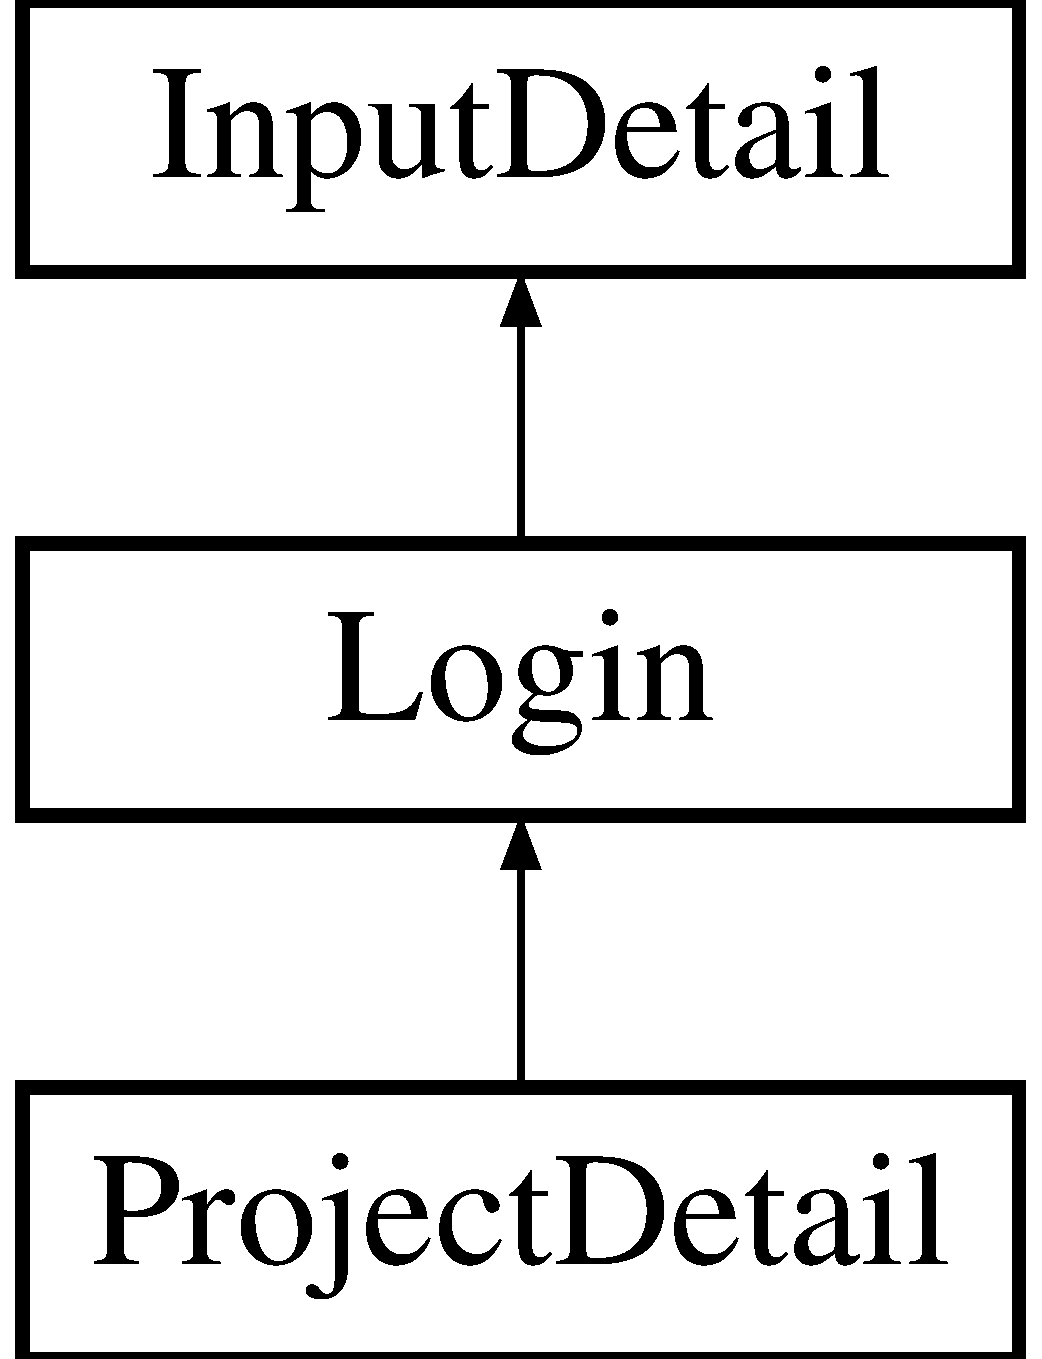
\includegraphics[height=3.000000cm]{dd/dfd/classLogin}
\end{center}
\end{figure}
\subsection*{\-Public \-Member \-Functions}
\begin{DoxyCompactItemize}
\item 
\hyperlink{classLogin_a4847f3e07e43b540d3339392346f87ff}{\-Login} ()
\begin{DoxyCompactList}\small\item\em \-Comstructor. \end{DoxyCompactList}\item 
void \hyperlink{classLogin_a2b2b36f506bcb5e7179b0b3afe164ace}{\-Login\-Page} (string \hyperlink{classInputDetail_a1abb16cd695678c3fa05e3c812823fee}{msg}=\char`\"{}\char`\"{}, string \hyperlink{classLogin_abea56d6d6403f1e627294f222dd77310}{email\-I\-D}=\char`\"{}abc@you.\-com\char`\"{}, string \hyperlink{classLogin_a39f7fd03b2b27c927c657ee73e7fcbbc}{password}=\char`\"{}\char`\"{})
\begin{DoxyCompactList}\small\item\em \-Function for creating login \-Page. \end{DoxyCompactList}\item 
void \hyperlink{classLogin_ab5bc65de431f277f15a3b423ad915808}{\-Read\-Login\-Detail} ()
\begin{DoxyCompactList}\small\item\em \-Reading login detail from text fields filled by user. \end{DoxyCompactList}\item 
void \hyperlink{classLogin_a3f4e5e4087c007e8e605849778881b39}{\-Registration\-Page} (string \hyperlink{classInputDetail_a1abb16cd695678c3fa05e3c812823fee}{msg}=\char`\"{}\char`\"{}, string \hyperlink{classLogin_abea56d6d6403f1e627294f222dd77310}{email\-I\-D}=\char`\"{}abc@you.\-com\char`\"{})
\begin{DoxyCompactList}\small\item\em \-For registering new user. \end{DoxyCompactList}\item 
void \hyperlink{classLogin_ae4f139afcb706f09b337befd123d5e18}{\-New\-User} ()
\begin{DoxyCompactList}\small\item\em \-Adding new user into database and if user already exists then move back to register page for unique email id. \end{DoxyCompactList}\item 
void \hyperlink{classLogin_ad127628ca09987d733477f90b828ad1e}{\-Select\-Login\-Detail} ()
\begin{DoxyCompactList}\small\item\em \-For reading email \-Id and password from \-User table in database. \end{DoxyCompactList}\item 
void \hyperlink{classLogin_a79ea5bbaeaa2ec6d21cd3195c522b863}{\-Confirm\-Page} (string \hyperlink{classInputDetail_a1abb16cd695678c3fa05e3c812823fee}{msg}=\char`\"{}\char`\"{}, string \hyperlink{classLogin_a39f7fd03b2b27c927c657ee73e7fcbbc}{password}=\char`\"{}\char`\"{}, string \hyperlink{classLogin_ade36f8943aafce470ef4b8353c79b2c6}{retype\-Password}=\char`\"{}\char`\"{})
\begin{DoxyCompactList}\small\item\em \-Page for validating email \-I\-D and setting user's password. \end{DoxyCompactList}\item 
void \hyperlink{classLogin_ac91737b2085d0b7e8943f49f2d08a0ff}{\-Add\-User} ()
\begin{DoxyCompactList}\small\item\em \-Add \-New user. \end{DoxyCompactList}\item 
void \hyperlink{classLogin_a4c5f4b15cce8b6bf325f35544f512fe2}{\-Reset\-Password\-Page} (string type=\char`\"{}1\char`\"{}, string \hyperlink{classInputDetail_a1abb16cd695678c3fa05e3c812823fee}{msg}=\char`\"{}\char`\"{}, string \hyperlink{classLogin_abea56d6d6403f1e627294f222dd77310}{email\-I\-D}=\char`\"{}abc@you.\-com\char`\"{})
\item 
void \hyperlink{classLogin_aa6978512971283a486347c3aa6ae0478}{\-Reset\-Password\-Form} (string type, string \hyperlink{classInputDetail_a1abb16cd695678c3fa05e3c812823fee}{msg}, string \hyperlink{classLogin_abea56d6d6403f1e627294f222dd77310}{email\-I\-D})
\item 
void \hyperlink{classLogin_a153d72df8d3333317e60219e8f6b8257}{\-Logout\-Page} ()
\begin{DoxyCompactList}\small\item\em \-Page for logging out. \end{DoxyCompactList}\item 
\hyperlink{classLogin_a659bc7233ec12c79b9fa523c1734fbbc}{$\sim$\-Login} ()
\end{DoxyCompactItemize}
\subsection*{\-Protected \-Attributes}
\begin{DoxyCompactItemize}
\item 
\-S\-T\-R\-I\-N\-G\-\_\-\-V\-E\-C \hyperlink{classLogin_abea56d6d6403f1e627294f222dd77310}{email\-I\-D}
\item 
\-S\-T\-R\-I\-N\-G\-\_\-\-V\-E\-C \hyperlink{classLogin_a39f7fd03b2b27c927c657ee73e7fcbbc}{password}
\item 
\-S\-T\-R\-I\-N\-G\-\_\-\-V\-E\-C \hyperlink{classLogin_ae22f0ed73e5248cd71a7b2167676376a}{reg\-Key}
\item 
string \hyperlink{classLogin_aa83b4706e0f0f0afc65f210ee8e4839a}{user\-Email\-I\-D}
\item 
string \hyperlink{classLogin_a9731be126468f535f161f045c95687c6}{user\-Password}
\item 
string \hyperlink{classLogin_ade36f8943aafce470ef4b8353c79b2c6}{retype\-Password}
\item 
string \hyperlink{classLogin_a624f15ecf989648b73a91743f67a6880}{current\-Time}
\item 
\hypertarget{classLogin_ab7769b44690490b43fc9046ad5958baf}{string {\bfseries key}}\label{dd/dfd/classLogin_ab7769b44690490b43fc9046ad5958baf}

\item 
\hypertarget{classLogin_a36ff1dd294aaaf884805325cee3b83d3}{\hyperlink{classSendMail}{\-Send\-Mail} {\bfseries send\-Mail}}\label{dd/dfd/classLogin_a36ff1dd294aaaf884805325cee3b83d3}

\end{DoxyCompactItemize}


\subsection{\-Detailed \-Description}
-\/-\/-\/-\/-\/-\/-\/-\/-\/-\/-\/-\/-\/-\/-\/-\/-\/-\/-\/-\/-\/-\/-\/-\/-\/-\/-\/-\/-\/-\/-\/-\/-\/-\/-\/-\/-\/-\/-\/-\/-\/-\/-\/-\/-\/-\/-\/-\/-\/-\/-\/-\/-\/-\/-\/-\/-\/-\/-\/-\/-\/-\/-\/-\/-\/-\/-\/ \-Include required header files -\/-\/-\/-\/-\/-\/-\/-\/-\/-\/-\/-\/-\/-\/-\/-\/-\/-\/-\/-\/-\/-\/-\/-\/-\/-\/-\/-\/-\/-\/-\/-\/-\/-\/-\/-\/-\/-\/-\/-\/-\/-\/-\/-\/-\/-\/-\/-\/-\/-\/-\/-\/-\/-\/-\/-\/-\/-\/-\/-\/-\/-\/-\/-\/-\/-\/ =================================================================== \-Class\-: \hyperlink{classLogin}{\-Login} \-Description\-: \hyperlink{classLogin}{\-Login} class for user login ===================================================================

\-Include \hyperlink{login_8h_source}{login.\-h} header file 

\-Definition at line 38 of file login.\-h.



\subsection{\-Constructor \& \-Destructor \-Documentation}
\hypertarget{classLogin_a4847f3e07e43b540d3339392346f87ff}{\index{\-Login@{\-Login}!\-Login@{\-Login}}
\index{\-Login@{\-Login}!Login@{\-Login}}
\subsubsection[{\-Login}]{\setlength{\rightskip}{0pt plus 5cm}{\bf \-Login\-::\-Login} (
\begin{DoxyParamCaption}
{}
\end{DoxyParamCaption}
)}}\label{dd/dfd/classLogin_a4847f3e07e43b540d3339392346f87ff}


\-Comstructor. 

\-Constructor 

\-Definition at line 32 of file login.\-cc.

\hypertarget{classLogin_a659bc7233ec12c79b9fa523c1734fbbc}{\index{\-Login@{\-Login}!$\sim$\-Login@{$\sim$\-Login}}
\index{$\sim$\-Login@{$\sim$\-Login}!Login@{\-Login}}
\subsubsection[{$\sim$\-Login}]{\setlength{\rightskip}{0pt plus 5cm}{\bf \-Login\-::$\sim$\-Login} (
\begin{DoxyParamCaption}
{}
\end{DoxyParamCaption}
)\hspace{0.3cm}{\ttfamily  \mbox{[}inline\mbox{]}}}}\label{dd/dfd/classLogin_a659bc7233ec12c79b9fa523c1734fbbc}
\-Destructor 

\-Definition at line 94 of file login.\-h.



\subsection{\-Member \-Function \-Documentation}
\hypertarget{classLogin_ac91737b2085d0b7e8943f49f2d08a0ff}{\index{\-Login@{\-Login}!\-Add\-User@{\-Add\-User}}
\index{\-Add\-User@{\-Add\-User}!Login@{\-Login}}
\subsubsection[{\-Add\-User}]{\setlength{\rightskip}{0pt plus 5cm}void {\bf \-Login\-::\-Add\-User} (
\begin{DoxyParamCaption}
{}
\end{DoxyParamCaption}
)}}\label{dd/dfd/classLogin_ac91737b2085d0b7e8943f49f2d08a0ff}


\-Add \-New user. 

\-Add new user 

\-Definition at line 273 of file login.\-cc.

\hypertarget{classLogin_a79ea5bbaeaa2ec6d21cd3195c522b863}{\index{\-Login@{\-Login}!\-Confirm\-Page@{\-Confirm\-Page}}
\index{\-Confirm\-Page@{\-Confirm\-Page}!Login@{\-Login}}
\subsubsection[{\-Confirm\-Page}]{\setlength{\rightskip}{0pt plus 5cm}void {\bf \-Login\-::\-Confirm\-Page} (
\begin{DoxyParamCaption}
\item[{string}]{msg = {\ttfamily \char`\"{}\char`\"{}}, }
\item[{string}]{password = {\ttfamily \char`\"{}\char`\"{}}, }
\item[{string}]{retype\-Password = {\ttfamily \char`\"{}\char`\"{}}}
\end{DoxyParamCaption}
)}}\label{dd/dfd/classLogin_a79ea5bbaeaa2ec6d21cd3195c522b863}


\-Page for validating email \-I\-D and setting user's password. 


\begin{DoxyParams}{\-Parameters}
{\em msg} & \-Shows error message \\
\hline
{\em password} & \-Password filled by user \\
\hline
{\em retype\-Password} & \-Password filled by user \\
\hline
\end{DoxyParams}


\-Definition at line 212 of file login.\-cc.

\hypertarget{classLogin_a2b2b36f506bcb5e7179b0b3afe164ace}{\index{\-Login@{\-Login}!\-Login\-Page@{\-Login\-Page}}
\index{\-Login\-Page@{\-Login\-Page}!Login@{\-Login}}
\subsubsection[{\-Login\-Page}]{\setlength{\rightskip}{0pt plus 5cm}void {\bf \-Login\-::\-Login\-Page} (
\begin{DoxyParamCaption}
\item[{string}]{msg = {\ttfamily \char`\"{}\char`\"{}}, }
\item[{string}]{email\-I\-D = {\ttfamily \char`\"{}abc@you.com\char`\"{}}, }
\item[{string}]{password = {\ttfamily \char`\"{}\char`\"{}}}
\end{DoxyParamCaption}
)}}\label{dd/dfd/classLogin_a2b2b36f506bcb5e7179b0b3afe164ace}


\-Function for creating login \-Page. 

\-Creating login page


\begin{DoxyParams}{\-Parameters}
{\em msg} & \-Show \-Message if email\-I\-D/ password incorrect \\
\hline
{\em emial\-I\-D} & user filled email id \\
\hline
{\em password} & uer password \\
\hline
\end{DoxyParams}


\-Definition at line 87 of file login.\-cc.

\hypertarget{classLogin_a153d72df8d3333317e60219e8f6b8257}{\index{\-Login@{\-Login}!\-Logout\-Page@{\-Logout\-Page}}
\index{\-Logout\-Page@{\-Logout\-Page}!Login@{\-Login}}
\subsubsection[{\-Logout\-Page}]{\setlength{\rightskip}{0pt plus 5cm}void {\bf \-Login\-::\-Logout\-Page} (
\begin{DoxyParamCaption}
{}
\end{DoxyParamCaption}
)}}\label{dd/dfd/classLogin_a153d72df8d3333317e60219e8f6b8257}


\-Page for logging out. 

\-Logout \-Page 

\-Definition at line 315 of file login.\-cc.

\hypertarget{classLogin_ae4f139afcb706f09b337befd123d5e18}{\index{\-Login@{\-Login}!\-New\-User@{\-New\-User}}
\index{\-New\-User@{\-New\-User}!Login@{\-Login}}
\subsubsection[{\-New\-User}]{\setlength{\rightskip}{0pt plus 5cm}void {\bf \-Login\-::\-New\-User} (
\begin{DoxyParamCaption}
{}
\end{DoxyParamCaption}
)}}\label{dd/dfd/classLogin_ae4f139afcb706f09b337befd123d5e18}


\-Adding new user into database and if user already exists then move back to register page for unique email id. 

\-Add new user in database 

\-Definition at line 172 of file login.\-cc.

\hypertarget{classLogin_ab5bc65de431f277f15a3b423ad915808}{\index{\-Login@{\-Login}!\-Read\-Login\-Detail@{\-Read\-Login\-Detail}}
\index{\-Read\-Login\-Detail@{\-Read\-Login\-Detail}!Login@{\-Login}}
\subsubsection[{\-Read\-Login\-Detail}]{\setlength{\rightskip}{0pt plus 5cm}void {\bf \-Login\-::\-Read\-Login\-Detail} (
\begin{DoxyParamCaption}
{}
\end{DoxyParamCaption}
)}}\label{dd/dfd/classLogin_ab5bc65de431f277f15a3b423ad915808}


\-Reading login detail from text fields filled by user. 

\-Read \hyperlink{classLogin}{\-Login} \-Detail


\begin{DoxyParams}{\-Parameters}
{\em } & \\
\hline
\end{DoxyParams}


\-Definition at line 71 of file login.\-cc.

\hypertarget{classLogin_a3f4e5e4087c007e8e605849778881b39}{\index{\-Login@{\-Login}!\-Registration\-Page@{\-Registration\-Page}}
\index{\-Registration\-Page@{\-Registration\-Page}!Login@{\-Login}}
\subsubsection[{\-Registration\-Page}]{\setlength{\rightskip}{0pt plus 5cm}void {\bf \-Login\-::\-Registration\-Page} (
\begin{DoxyParamCaption}
\item[{string}]{msg = {\ttfamily \char`\"{}\char`\"{}}, }
\item[{string}]{email\-I\-D = {\ttfamily \char`\"{}abc@you.com\char`\"{}}}
\end{DoxyParamCaption}
)}}\label{dd/dfd/classLogin_a3f4e5e4087c007e8e605849778881b39}


\-For registering new user. 

\-Register user page 

\-Definition at line 131 of file login.\-cc.

\hypertarget{classLogin_aa6978512971283a486347c3aa6ae0478}{\index{\-Login@{\-Login}!\-Reset\-Password\-Form@{\-Reset\-Password\-Form}}
\index{\-Reset\-Password\-Form@{\-Reset\-Password\-Form}!Login@{\-Login}}
\subsubsection[{\-Reset\-Password\-Form}]{\setlength{\rightskip}{0pt plus 5cm}void {\bf \-Login\-::\-Reset\-Password\-Form} (
\begin{DoxyParamCaption}
\item[{string}]{type, }
\item[{string}]{msg, }
\item[{string}]{email\-I\-D}
\end{DoxyParamCaption}
)}}\label{dd/dfd/classLogin_aa6978512971283a486347c3aa6ae0478}
\-Reset \-Password \-Forms 

\-Definition at line 347 of file login.\-cc.

\hypertarget{classLogin_a4c5f4b15cce8b6bf325f35544f512fe2}{\index{\-Login@{\-Login}!\-Reset\-Password\-Page@{\-Reset\-Password\-Page}}
\index{\-Reset\-Password\-Page@{\-Reset\-Password\-Page}!Login@{\-Login}}
\subsubsection[{\-Reset\-Password\-Page}]{\setlength{\rightskip}{0pt plus 5cm}void {\bf \-Login\-::\-Reset\-Password\-Page} (
\begin{DoxyParamCaption}
\item[{string}]{type = {\ttfamily \char`\"{}1\char`\"{}}, }
\item[{string}]{msg = {\ttfamily \char`\"{}\char`\"{}}, }
\item[{string}]{email\-I\-D = {\ttfamily \char`\"{}abc@you.com\char`\"{}}}
\end{DoxyParamCaption}
)}}\label{dd/dfd/classLogin_a4c5f4b15cce8b6bf325f35544f512fe2}
\-Reset password of existing user 

\-Definition at line 325 of file login.\-cc.

\hypertarget{classLogin_ad127628ca09987d733477f90b828ad1e}{\index{\-Login@{\-Login}!\-Select\-Login\-Detail@{\-Select\-Login\-Detail}}
\index{\-Select\-Login\-Detail@{\-Select\-Login\-Detail}!Login@{\-Login}}
\subsubsection[{\-Select\-Login\-Detail}]{\setlength{\rightskip}{0pt plus 5cm}void {\bf \-Login\-::\-Select\-Login\-Detail} (
\begin{DoxyParamCaption}
{}
\end{DoxyParamCaption}
)}}\label{dd/dfd/classLogin_ad127628ca09987d733477f90b828ad1e}


\-For reading email \-Id and password from \-User table in database. 

\-For selecting emial and password fron user table 

\-Definition at line 44 of file login.\-cc.



\subsection{\-Member \-Data \-Documentation}
\hypertarget{classLogin_a624f15ecf989648b73a91743f67a6880}{\index{\-Login@{\-Login}!current\-Time@{current\-Time}}
\index{current\-Time@{current\-Time}!Login@{\-Login}}
\subsubsection[{current\-Time}]{\setlength{\rightskip}{0pt plus 5cm}string {\bf \-Login\-::current\-Time}\hspace{0.3cm}{\ttfamily  \mbox{[}protected\mbox{]}}}}\label{dd/dfd/classLogin_a624f15ecf989648b73a91743f67a6880}
\-Currennt \-Time 

\-Definition at line 51 of file login.\-h.

\hypertarget{classLogin_abea56d6d6403f1e627294f222dd77310}{\index{\-Login@{\-Login}!email\-I\-D@{email\-I\-D}}
\index{email\-I\-D@{email\-I\-D}!Login@{\-Login}}
\subsubsection[{email\-I\-D}]{\setlength{\rightskip}{0pt plus 5cm}\-S\-T\-R\-I\-N\-G\-\_\-\-V\-E\-C {\bf \-Login\-::email\-I\-D}\hspace{0.3cm}{\ttfamily  \mbox{[}protected\mbox{]}}}}\label{dd/dfd/classLogin_abea56d6d6403f1e627294f222dd77310}
\-For storting email and password of users \-Email \-I\-D as vector 

\-Reimplemented from \hyperlink{classInputDetail_ad3f1db4fddbe0d4efbf1d5bc74d52257}{\-Input\-Detail}.



\-Definition at line 43 of file login.\-h.

\hypertarget{classLogin_a39f7fd03b2b27c927c657ee73e7fcbbc}{\index{\-Login@{\-Login}!password@{password}}
\index{password@{password}!Login@{\-Login}}
\subsubsection[{password}]{\setlength{\rightskip}{0pt plus 5cm}\-S\-T\-R\-I\-N\-G\-\_\-\-V\-E\-C {\bf \-Login\-::password}\hspace{0.3cm}{\ttfamily  \mbox{[}protected\mbox{]}}}}\label{dd/dfd/classLogin_a39f7fd03b2b27c927c657ee73e7fcbbc}
password as vector variable 

\-Definition at line 43 of file login.\-h.

\hypertarget{classLogin_ae22f0ed73e5248cd71a7b2167676376a}{\index{\-Login@{\-Login}!reg\-Key@{reg\-Key}}
\index{reg\-Key@{reg\-Key}!Login@{\-Login}}
\subsubsection[{reg\-Key}]{\setlength{\rightskip}{0pt plus 5cm}\-S\-T\-R\-I\-N\-G\-\_\-\-V\-E\-C {\bf \-Login\-::reg\-Key}\hspace{0.3cm}{\ttfamily  \mbox{[}protected\mbox{]}}}}\label{dd/dfd/classLogin_ae22f0ed73e5248cd71a7b2167676376a}
\-Registration key 

\-Definition at line 43 of file login.\-h.

\hypertarget{classLogin_ade36f8943aafce470ef4b8353c79b2c6}{\index{\-Login@{\-Login}!retype\-Password@{retype\-Password}}
\index{retype\-Password@{retype\-Password}!Login@{\-Login}}
\subsubsection[{retype\-Password}]{\setlength{\rightskip}{0pt plus 5cm}string {\bf \-Login\-::retype\-Password}\hspace{0.3cm}{\ttfamily  \mbox{[}protected\mbox{]}}}}\label{dd/dfd/classLogin_ade36f8943aafce470ef4b8353c79b2c6}
\-For reading password 

\-Definition at line 47 of file login.\-h.

\hypertarget{classLogin_aa83b4706e0f0f0afc65f210ee8e4839a}{\index{\-Login@{\-Login}!user\-Email\-I\-D@{user\-Email\-I\-D}}
\index{user\-Email\-I\-D@{user\-Email\-I\-D}!Login@{\-Login}}
\subsubsection[{user\-Email\-I\-D}]{\setlength{\rightskip}{0pt plus 5cm}string {\bf \-Login\-::user\-Email\-I\-D}\hspace{0.3cm}{\ttfamily  \mbox{[}protected\mbox{]}}}}\label{dd/dfd/classLogin_aa83b4706e0f0f0afc65f210ee8e4839a}
\-For reading email\-I\-D in text field 

\-Definition at line 47 of file login.\-h.

\hypertarget{classLogin_a9731be126468f535f161f045c95687c6}{\index{\-Login@{\-Login}!user\-Password@{user\-Password}}
\index{user\-Password@{user\-Password}!Login@{\-Login}}
\subsubsection[{user\-Password}]{\setlength{\rightskip}{0pt plus 5cm}string {\bf \-Login\-::user\-Password}\hspace{0.3cm}{\ttfamily  \mbox{[}protected\mbox{]}}}}\label{dd/dfd/classLogin_a9731be126468f535f161f045c95687c6}
\-For reading password in text field 

\-Definition at line 47 of file login.\-h.



\-The documentation for this class was generated from the following files\-:\begin{DoxyCompactItemize}
\item 
frontend/src/header/login.\-h\item 
frontend/src/login.\-cc\end{DoxyCompactItemize}

\hypertarget{classMD5}{\section{M\-D5 Class Reference}
\label{classMD5}\index{M\-D5@{M\-D5}}
}
\subsection*{Public Types}
\begin{DoxyCompactItemize}
\item 
\hypertarget{classMD5_aa836972700679dbcff6ae8337f6db464}{typedef unsigned int {\bfseries size\-\_\-type}}\label{classMD5_aa836972700679dbcff6ae8337f6db464}

\end{DoxyCompactItemize}
\subsection*{Public Member Functions}
\begin{DoxyCompactItemize}
\item 
\hypertarget{classMD5_a155356ffd713345e69e6dcbd9f8da6ce}{{\bfseries M\-D5} (const std\-::string \&text)}\label{classMD5_a155356ffd713345e69e6dcbd9f8da6ce}

\item 
\hypertarget{classMD5_ac5ddf6cd8f940422396d321ea90ed045}{void {\bfseries update} (const unsigned char $\ast$buf, size\-\_\-type length)}\label{classMD5_ac5ddf6cd8f940422396d321ea90ed045}

\item 
\hypertarget{classMD5_ac5ccba375539b993958fb235f8ac849c}{void {\bfseries update} (const char $\ast$buf, size\-\_\-type length)}\label{classMD5_ac5ccba375539b993958fb235f8ac849c}

\item 
\hypertarget{classMD5_a10f607494a3f2e3e515fc4b99d1a06cc}{\hyperlink{classMD5}{M\-D5} \& {\bfseries finalize} ()}\label{classMD5_a10f607494a3f2e3e515fc4b99d1a06cc}

\item 
\hypertarget{classMD5_ad36c65acf87e397bf717bc3defbc0c7a}{std\-::string {\bfseries hexdigest} () const }\label{classMD5_ad36c65acf87e397bf717bc3defbc0c7a}

\end{DoxyCompactItemize}
\subsection*{Friends}
\begin{DoxyCompactItemize}
\item 
\hypertarget{classMD5_a0739666fd0f3a7117546f6c50e0783b2}{std\-::ostream \& {\bfseries operator$<$$<$} (std\-::ostream \&, \hyperlink{classMD5}{M\-D5} md5)}\label{classMD5_a0739666fd0f3a7117546f6c50e0783b2}

\end{DoxyCompactItemize}


\subsection{Detailed Description}


Definition at line 69 of file md5.\-h.



The documentation for this class was generated from the following files\-:\begin{DoxyCompactItemize}
\item 
src/header/md5.\-h\item 
src/md5.\-cc\end{DoxyCompactItemize}

\hypertarget{classPageLayout}{\section{Page\-Layout Class Reference}
\label{classPageLayout}\index{Page\-Layout@{Page\-Layout}}
}


{\ttfamily \#include $<$pagelayout.\-h$>$}

Inheritance diagram for Page\-Layout\-:\begin{figure}[H]
\begin{center}
\leavevmode
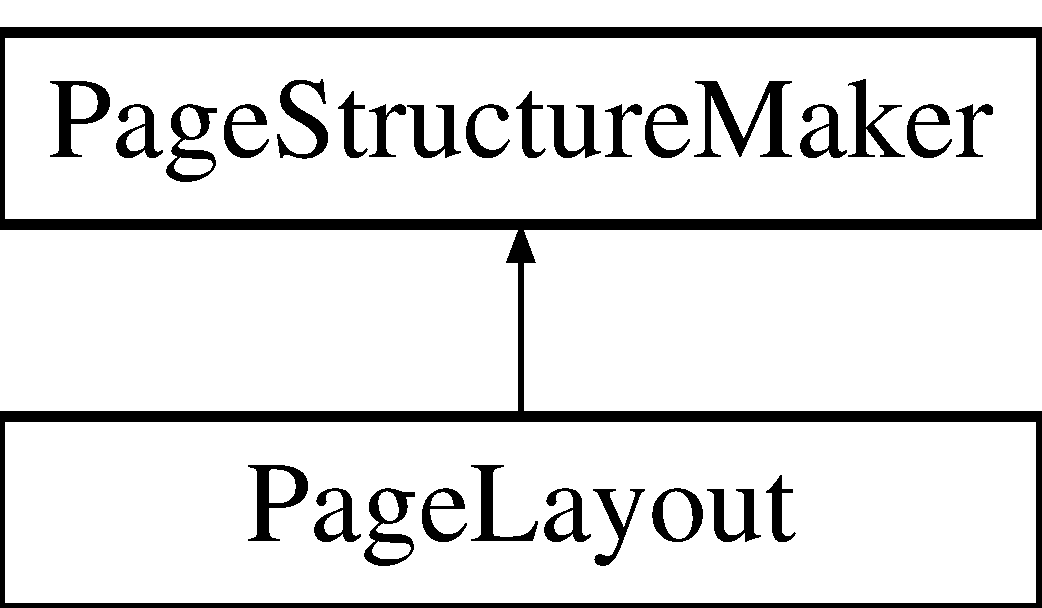
\includegraphics[height=5.000000cm]{classPageLayout}
\end{center}
\end{figure}
\subsection*{Public Member Functions}
\begin{DoxyCompactItemize}
\item 
\hyperlink{classPageLayout_ab3f470f006f9820610d9aaebe5b8427b}{Page\-Layout} ()
\item 
void \hyperlink{classPageLayout_a7726061f0653245f644a05807fa92472}{Header} ()
\item 
void \hyperlink{classPageLayout_a68aa868a8868b12964f161838b5f814c}{Footer} ()
\item 
void \hyperlink{classPageLayout_a49af1dca286bbee9432192a7b3c00332}{Menu} ()
\item 
void \hyperlink{classPageLayout_ae60235c6af48e3ebbc6343d02456da0c}{Logo} (string logo\-Name)
\item 
void \hyperlink{classPageLayout_ae50907d56f0ba7a85f7ccfdeafa45bcc}{Head} (string title\-Name)
\item 
void \hyperlink{classPageLayout_a449b4dde24cf3dc10299dc3c7bfc0e9c}{Set\-Cookies} (string email\-I\-D, string \hyperlink{classPageLayout_ab796c4a12a3f9c089881085e508e2a1c}{session\-I\-D})
\item 
void \hyperlink{classPageLayout_a9884173383d3e9b91e5b4ba6a619caa9}{Context\-Type} ()
\item 
void \hyperlink{classPageLayout_abe2cfa43480c1b48125b3d618cab7831}{Logout\-Link} ()
\item 
void \hyperlink{classPageStructureMaker_aaf78d67380c400cc0057c6519276f721}{Set\-H\-T\-M\-L\-Variables} ()
\item 
void \hyperlink{classPageStructureMaker_ad25d6abc983253567e2370882fc1b407}{H\-T\-M\-L\-Start} ()
\item 
void \hyperlink{classPageStructureMaker_a63b877af1c2c8de8332e3f7eb4c2c2b0}{H\-T\-M\-L\-End} ()
\item 
void \hyperlink{classPageStructureMaker_a14312134cb108f91f2e6d9cbd6916e97}{Head\-Start} ()
\item 
void \hyperlink{classPageStructureMaker_ad64115d592b0989b422a93f85278186e}{Head\-End} ()
\item 
void \hyperlink{classPageStructureMaker_a81e902ddc0c0287df1ba0f614a3774d6}{Title} (string page\-Title)
\item 
void \hyperlink{classPageStructureMaker_aacdb11817f8ab246bc59c552e04e862d}{C\-S\-S} (string href)
\item 
void \hyperlink{classPageStructureMaker_ac221d1169f4dbcef6adb00938919193d}{Javascript} (string src)
\item 
void \hyperlink{classPageStructureMaker_ab7a645675166f34fac99f1ed8feb7c27}{Body\-Start} ()
\item 
void \hyperlink{classPageStructureMaker_ac91e234e2d54dedd9d7e556fabf21d2b}{Body\-End} ()
\item 
void \hyperlink{classPageStructureMaker_a927f92889555dd316c129f706be86a5c}{Div\-Start} (string id, string class\-Name)
\item 
void \hyperlink{classPageStructureMaker_a2913e76bf188ed777dcd33003ef6207d}{Div\-End} ()
\item 
void \hyperlink{classPageStructureMaker_a3f25d5b844a2251883acb80d8fabb77d}{Form\-Start} (string name, string action, string method)
\item 
void \hyperlink{classPageStructureMaker_a65d97f23bb543f3db5201b2009f7f65a}{Form\-End} ()
\item 
void \hyperlink{classPageStructureMaker_a04e68e69005f3933e0f496c3db474daf}{Table\-Start} (string id, string class\-Name)
\item 
void \hyperlink{classPageStructureMaker_a7f8fefbe7a825c1b7761fc8a0f1bb8e4}{Table\-End} ()
\item 
void \hyperlink{classPageStructureMaker_ac24ce26202757aaa30402155daf8a3d0}{List\-Start} (string list\-Type)
\item 
void \hyperlink{classPageStructureMaker_a8578b1555ad2fc92a9efc7dbf7d1fe87}{List\-End} (string list\-Type)
\item 
void \hyperlink{classPageStructureMaker_adf4116e526026edc3c8a3bcf96a7e929}{List\-Item} (string list\-Item)
\item 
void \hyperlink{classPageStructureMaker_a8c0fae5b599182863066de56ae0cea42}{Anchor} (string href, string target)
\item 
void \hyperlink{classPageStructureMaker_a3547027801e298307527f1e934787b13}{Input\-Field} (string type, string name, int name\-No, string value)
\item 
void \hyperlink{classPageStructureMaker_a928ea6f84a8f7833c128034068a4b9a7}{Input\-Field} (string type, string name, string value)
\item 
void \hyperlink{classPageStructureMaker_ae8684bb66ca463e2f92e09c96137f9e3}{Select\-Field\-Start} (string name)
\item 
void \hyperlink{classPageStructureMaker_a81eb3cdbc840a4c8165cef87330ade09}{Select\-Field\-End} ()
\item 
void \hyperlink{classPageStructureMaker_a77856078e74dab25329132ea07466f92}{Select\-Option\-Start} (string value, string selected)
\item 
void \hyperlink{classPageStructureMaker_a7682f479f7f1012d426ec9f9535def60}{Select\-Option\-End} ()
\item 
void \hyperlink{classPageStructureMaker_a419feca1cfdb50e1be757eb1c2707a73}{Button} (string id, string type, string class\-Name, string value)
\end{DoxyCompactItemize}
\subsection*{Protected Attributes}
\begin{DoxyCompactItemize}
\item 
\hypertarget{classPageLayout_a8a3c1ddc422df2556fbc95d0cd575a05}{string {\bfseries project\-Name}}\label{classPageLayout_a8a3c1ddc422df2556fbc95d0cd575a05}

\item 
\hypertarget{classPageLayout_a9abec89a54a6f0dac84114919d2ad117}{ifstream {\bfseries in\-File}}\label{classPageLayout_a9abec89a54a6f0dac84114919d2ad117}

\item 
\hypertarget{classPageLayout_ad52913274f786e82e1e09f5df4bf5347}{ofstream {\bfseries out\-File}}\label{classPageLayout_ad52913274f786e82e1e09f5df4bf5347}

\item 
string \hyperlink{classPageLayout_ab796c4a12a3f9c089881085e508e2a1c}{session\-I\-D}
\item 
string \hyperlink{classPageStructureMaker_af41d4e21b808f5f8dc2c727f775b6fb2}{start\-H1}
\item 
\hypertarget{classPageStructureMaker_a3786a6f477632e4a60205a988d6b599d}{string {\bfseries end\-H1}}\label{classPageStructureMaker_a3786a6f477632e4a60205a988d6b599d}

\item 
\hypertarget{classPageStructureMaker_adb966c147c6328c8e48281c882de776d}{string {\bfseries start\-H3}}\label{classPageStructureMaker_adb966c147c6328c8e48281c882de776d}

\item 
\hypertarget{classPageStructureMaker_a22e6bf3eb787284b745d694613c1d9da}{string {\bfseries end\-H3}}\label{classPageStructureMaker_a22e6bf3eb787284b745d694613c1d9da}

\item 
\hypertarget{classPageStructureMaker_a7e458e675a3adf987a153e08f3795941}{string {\bfseries start\-T\-D}}\label{classPageStructureMaker_a7e458e675a3adf987a153e08f3795941}

\item 
\hypertarget{classPageStructureMaker_ad27f03939a04048a03be0f1bb8edd38a}{string {\bfseries end\-T\-D}}\label{classPageStructureMaker_ad27f03939a04048a03be0f1bb8edd38a}

\item 
\hypertarget{classPageStructureMaker_a4fe234b016efcb9eaa757879b8858190}{string {\bfseries start\-T\-H}}\label{classPageStructureMaker_a4fe234b016efcb9eaa757879b8858190}

\item 
\hypertarget{classPageStructureMaker_aa244b4ef71850dc76fcfb5157bcaf8fc}{string {\bfseries end\-T\-H}}\label{classPageStructureMaker_aa244b4ef71850dc76fcfb5157bcaf8fc}

\item 
\hypertarget{classPageStructureMaker_aa59b4949d26fab5a72710fa9fc3e8ea9}{string {\bfseries start\-T\-R}}\label{classPageStructureMaker_aa59b4949d26fab5a72710fa9fc3e8ea9}

\item 
\hypertarget{classPageStructureMaker_afee49ebdcbc0971142fcf7eae8baa306}{string {\bfseries end\-T\-R}}\label{classPageStructureMaker_afee49ebdcbc0971142fcf7eae8baa306}

\item 
\hypertarget{classPageStructureMaker_aa0f624b485f07f6e19151b1df3dc59a3}{string {\bfseries start\-B}}\label{classPageStructureMaker_aa0f624b485f07f6e19151b1df3dc59a3}

\item 
\hypertarget{classPageStructureMaker_ad46c3195310a1f0226e21d2eb5befb00}{string {\bfseries end\-B}}\label{classPageStructureMaker_ad46c3195310a1f0226e21d2eb5befb00}

\item 
\hypertarget{classPageStructureMaker_a63911cb925ccdc6c879905a677ed8881}{string {\bfseries brk}}\label{classPageStructureMaker_a63911cb925ccdc6c879905a677ed8881}

\end{DoxyCompactItemize}


\subsection{Detailed Description}
-\/-\/-\/-\/-\/-\/-\/-\/-\/-\/-\/-\/-\/-\/-\/-\/-\/-\/-\/-\/-\/-\/-\/-\/-\/-\/-\/-\/-\/-\/-\/-\/-\/-\/-\/-\/-\/-\/-\/-\/-\/-\/-\/-\/-\/-\/-\/-\/-\/-\/-\/-\/-\/-\/-\/-\/-\/-\/-\/-\/-\/-\/-\/-\/-\/-\/-\/ Include required header files ------------------------------------------------------------------ =================================================================== Class\-: \hyperlink{classPageLayout}{Page\-Layout} \-: public \hyperlink{classPageStructureMaker}{Page\-Structure\-Maker} Description\-: For adding header and footer to page =================================================================== 

Definition at line 33 of file pagelayout.\-h.



\subsection{Constructor \& Destructor Documentation}
\hypertarget{classPageLayout_ab3f470f006f9820610d9aaebe5b8427b}{\index{Page\-Layout@{Page\-Layout}!Page\-Layout@{Page\-Layout}}
\index{Page\-Layout@{Page\-Layout}!PageLayout@{Page\-Layout}}
\subsubsection[{Page\-Layout}]{\setlength{\rightskip}{0pt plus 5cm}Page\-Layout\-::\-Page\-Layout (
\begin{DoxyParamCaption}
{}
\end{DoxyParamCaption}
)}}\label{classPageLayout_ab3f470f006f9820610d9aaebe5b8427b}
Constructor

-\/-\/-\/-\/-\/-\/-\/-\/-\/-\/-\/-\/-\/-\/-\/-\/-\/-\/-\/-\/-\/-\/-\/-\/-\/-\/-\/-\/-\/-\/-\/-\/-\/-\/-\/-\/-\/-\/-\/-\/-\/-\/-\/-\/-\/-\/-\/-\/-\/-\/-\/-\/-\/-\/-\/-\/-\/-\/-\/-\/-\/-\/-\/-\/-\/-\/-\/ Include local header file ------------------------------------------------------------------ -\/-\/-\/-\/-\/-\/-\/-\/-\/-\/-\/-\/-\/-\/-\/-\/-\/-\/-\/-\/-\/-\/-\/-\/-\/-\/-\/-\/-\/-\/-\/-\/-\/-\/-\/-\/-\/-\/-\/-\/-\/-\/-\/-\/-\/-\/-\/-\/-\/-\/-\/-\/-\/-\/-\/-\/-\/-\/-\/-\/-\/-\/-\/-\/-\/-\/-\/ Function Definitions of \hyperlink{classPageLayout}{Page\-Layout} Class ------------------------------------------------------------------ -\/-\/-\/-\/-\/-\/-\/-\/-\/-\/-\/-\/-\/-\/-\/-\/-\/-\/-\/-\/-\/-\/-\/-\/-\/-\/-\/-\/-\/-\/-\/-\/-\/-\/-\/-\/-\/-\/-\/-\/-\/-\/-\/-\/-\/-\/-\/-\/-\/-\/-\/-\/-\/-\/-\/-\/-\/-\/-\/-\/-\/-\/-\/-\/-\/-\/-\/-\/ Class\-: \hyperlink{classPageLayout}{Page\-Layout} Method\-: \hyperlink{classPageLayout}{Page\-Layout} \-:\-: \hyperlink{classPageLayout_ab3f470f006f9820610d9aaebe5b8427b}{Page\-Layout()} Description\-: Constructor -\/-\/-\/-\/-\/-\/-\/-\/-\/-\/-\/-\/-\/-\/-\/-\/-\/-\/-\/-\/-\/-\/-\/-\/-\/-\/-\/-\/-\/-\/-\/-\/-\/-\/-\/-\/-\/-\/-\/-\/-\/-\/-\/-\/-\/-\/-\/-\/-\/-\/-\/-\/-\/-\/-\/-\/-\/-\/-\/-\/-\/-\/-\/-\/-\/-\/-\/-\/ 

Definition at line 38 of file pagelayout.\-cc.



\subsection{Member Function Documentation}
\hypertarget{classPageStructureMaker_a8c0fae5b599182863066de56ae0cea42}{\index{Page\-Layout@{Page\-Layout}!Anchor@{Anchor}}
\index{Anchor@{Anchor}!PageLayout@{Page\-Layout}}
\subsubsection[{Anchor}]{\setlength{\rightskip}{0pt plus 5cm}void Page\-Structure\-Maker\-::\-Anchor (
\begin{DoxyParamCaption}
\item[{string}]{href, }
\item[{string}]{target}
\end{DoxyParamCaption}
)\hspace{0.3cm}{\ttfamily [inherited]}}}\label{classPageStructureMaker_a8c0fae5b599182863066de56ae0cea42}
Anchor Tag

--------------------------------------------------------------------\par
 Class\-: \hyperlink{classPageStructureMaker}{Page\-Structure\-Maker} \par
 Method\-: \hyperlink{classPageStructureMaker}{Page\-Structure\-Maker} \-:\-: Anchor(string href) \par
 Description\-: Anchor Tag \par
 -\/-\/-\/-\/-\/-\/-\/-\/-\/-\/-\/-\/-\/-\/-\/-\/-\/-\/-\/-\/-\/-\/-\/-\/-\/-\/-\/-\/-\/-\/-\/-\/-\/-\/-\/-\/-\/-\/-\/-\/-\/-\/-\/-\/-\/-\/-\/-\/-\/-\/-\/-\/-\/-\/-\/-\/-\/-\/-\/-\/-\/-\/-\/-\/-\/-\/-\/-\/ 

Definition at line 318 of file pagestructure.\-cc.

\hypertarget{classPageStructureMaker_ac91e234e2d54dedd9d7e556fabf21d2b}{\index{Page\-Layout@{Page\-Layout}!Body\-End@{Body\-End}}
\index{Body\-End@{Body\-End}!PageLayout@{Page\-Layout}}
\subsubsection[{Body\-End}]{\setlength{\rightskip}{0pt plus 5cm}void Page\-Structure\-Maker\-::\-Body\-End (
\begin{DoxyParamCaption}
{}
\end{DoxyParamCaption}
)\hspace{0.3cm}{\ttfamily [inherited]}}}\label{classPageStructureMaker_ac91e234e2d54dedd9d7e556fabf21d2b}
Display $<$/\-B\-O\-D\-Y$>$

-\/-\/-\/-\/-\/-\/-\/-\/-\/-\/-\/-\/-\/-\/-\/-\/-\/-\/-\/-\/-\/-\/-\/-\/-\/-\/-\/-\/-\/-\/-\/-\/-\/-\/-\/-\/-\/-\/-\/-\/-\/-\/-\/-\/-\/-\/-\/-\/-\/-\/-\/-\/-\/-\/-\/-\/-\/-\/-\/-\/-\/-\/-\/-\/-\/-\/-\/-\/ Class\-: \hyperlink{classPageStructureMaker}{Page\-Structure\-Maker} Method\-: \hyperlink{classPageStructureMaker}{Page\-Structure\-Maker} \-:\-: \hyperlink{classPageStructureMaker_ac91e234e2d54dedd9d7e556fabf21d2b}{Body\-End()} Description\-: Display $<$/\-B\-O\-D\-Y$>$ -\/-\/-\/-\/-\/-\/-\/-\/-\/-\/-\/-\/-\/-\/-\/-\/-\/-\/-\/-\/-\/-\/-\/-\/-\/-\/-\/-\/-\/-\/-\/-\/-\/-\/-\/-\/-\/-\/-\/-\/-\/-\/-\/-\/-\/-\/-\/-\/-\/-\/-\/-\/-\/-\/-\/-\/-\/-\/-\/-\/-\/-\/-\/-\/-\/-\/-\/-\/ 

Definition at line 180 of file pagestructure.\-cc.

\hypertarget{classPageStructureMaker_ab7a645675166f34fac99f1ed8feb7c27}{\index{Page\-Layout@{Page\-Layout}!Body\-Start@{Body\-Start}}
\index{Body\-Start@{Body\-Start}!PageLayout@{Page\-Layout}}
\subsubsection[{Body\-Start}]{\setlength{\rightskip}{0pt plus 5cm}void Page\-Structure\-Maker\-::\-Body\-Start (
\begin{DoxyParamCaption}
{}
\end{DoxyParamCaption}
)\hspace{0.3cm}{\ttfamily [inherited]}}}\label{classPageStructureMaker_ab7a645675166f34fac99f1ed8feb7c27}
Display $<$\-B\-O\-D\-Y$>$

-\/-\/-\/-\/-\/-\/-\/-\/-\/-\/-\/-\/-\/-\/-\/-\/-\/-\/-\/-\/-\/-\/-\/-\/-\/-\/-\/-\/-\/-\/-\/-\/-\/-\/-\/-\/-\/-\/-\/-\/-\/-\/-\/-\/-\/-\/-\/-\/-\/-\/-\/-\/-\/-\/-\/-\/-\/-\/-\/-\/-\/-\/-\/-\/-\/-\/-\/-\/ Class\-: \hyperlink{classPageStructureMaker}{Page\-Structure\-Maker} Method\-: \hyperlink{classPageStructureMaker}{Page\-Structure\-Maker} \-:\-: \hyperlink{classPageStructureMaker_ab7a645675166f34fac99f1ed8feb7c27}{Body\-Start()} Description\-: Display $<$B\-O\-D\-Y$>$ -\/-\/-\/-\/-\/-\/-\/-\/-\/-\/-\/-\/-\/-\/-\/-\/-\/-\/-\/-\/-\/-\/-\/-\/-\/-\/-\/-\/-\/-\/-\/-\/-\/-\/-\/-\/-\/-\/-\/-\/-\/-\/-\/-\/-\/-\/-\/-\/-\/-\/-\/-\/-\/-\/-\/-\/-\/-\/-\/-\/-\/-\/-\/-\/-\/-\/-\/-\/ 

Definition at line 166 of file pagestructure.\-cc.

\hypertarget{classPageStructureMaker_a419feca1cfdb50e1be757eb1c2707a73}{\index{Page\-Layout@{Page\-Layout}!Button@{Button}}
\index{Button@{Button}!PageLayout@{Page\-Layout}}
\subsubsection[{Button}]{\setlength{\rightskip}{0pt plus 5cm}void Page\-Structure\-Maker\-::\-Button (
\begin{DoxyParamCaption}
\item[{string}]{id, }
\item[{string}]{type, }
\item[{string}]{class\-Name, }
\item[{string}]{value}
\end{DoxyParamCaption}
)\hspace{0.3cm}{\ttfamily [inherited]}}}\label{classPageStructureMaker_a419feca1cfdb50e1be757eb1c2707a73}
Button

-\/-\/-\/-\/-\/-\/-\/-\/-\/-\/-\/-\/-\/-\/-\/-\/-\/-\/-\/-\/-\/-\/-\/-\/-\/-\/-\/-\/-\/-\/-\/-\/-\/-\/-\/-\/-\/-\/-\/-\/-\/-\/-\/-\/-\/-\/-\/-\/-\/-\/-\/-\/-\/-\/-\/-\/-\/-\/-\/-\/-\/-\/-\/-\/-\/-\/-\/-\/ Class\-: \hyperlink{classPageStructureMaker}{Page\-Structure\-Maker} Method\-: \hyperlink{classPageStructureMaker}{Page\-Structure\-Maker} \-:\-: Button(string id, string type, string class\-Name, string value) Description\-: Create button(next, submit, etc) -\/-\/-\/-\/-\/-\/-\/-\/-\/-\/-\/-\/-\/-\/-\/-\/-\/-\/-\/-\/-\/-\/-\/-\/-\/-\/-\/-\/-\/-\/-\/-\/-\/-\/-\/-\/-\/-\/-\/-\/-\/-\/-\/-\/-\/-\/-\/-\/-\/-\/-\/-\/-\/-\/-\/-\/-\/-\/-\/-\/-\/-\/-\/-\/-\/-\/-\/-\/ 

Definition at line 436 of file pagestructure.\-cc.

\hypertarget{classPageLayout_a9884173383d3e9b91e5b4ba6a619caa9}{\index{Page\-Layout@{Page\-Layout}!Context\-Type@{Context\-Type}}
\index{Context\-Type@{Context\-Type}!PageLayout@{Page\-Layout}}
\subsubsection[{Context\-Type}]{\setlength{\rightskip}{0pt plus 5cm}void Page\-Layout\-::\-Context\-Type (
\begin{DoxyParamCaption}
{}
\end{DoxyParamCaption}
)}}\label{classPageLayout_a9884173383d3e9b91e5b4ba6a619caa9}
Context-\/\-Type header

--------------------------------------------------------------------\par
 Class\-: \hyperlink{classPageLayout}{Page\-Layout} \par
 Method\-: \hyperlink{classPageLayout}{Page\-Layout} \-:\-: Context\-Type \par
 Description\-: Setting content-\/type header \par
 -\/-\/-\/-\/-\/-\/-\/-\/-\/-\/-\/-\/-\/-\/-\/-\/-\/-\/-\/-\/-\/-\/-\/-\/-\/-\/-\/-\/-\/-\/-\/-\/-\/-\/-\/-\/-\/-\/-\/-\/-\/-\/-\/-\/-\/-\/-\/-\/-\/-\/-\/-\/-\/-\/-\/-\/-\/-\/-\/-\/-\/-\/-\/-\/-\/-\/-\/-\/ 

Definition at line 162 of file pagelayout.\-cc.

\hypertarget{classPageStructureMaker_aacdb11817f8ab246bc59c552e04e862d}{\index{Page\-Layout@{Page\-Layout}!C\-S\-S@{C\-S\-S}}
\index{C\-S\-S@{C\-S\-S}!PageLayout@{Page\-Layout}}
\subsubsection[{C\-S\-S}]{\setlength{\rightskip}{0pt plus 5cm}void Page\-Structure\-Maker\-::\-C\-S\-S (
\begin{DoxyParamCaption}
\item[{string}]{href}
\end{DoxyParamCaption}
)\hspace{0.3cm}{\ttfamily [inherited]}}}\label{classPageStructureMaker_aacdb11817f8ab246bc59c552e04e862d}
Add External C\-S\-S

-\/-\/-\/-\/-\/-\/-\/-\/-\/-\/-\/-\/-\/-\/-\/-\/-\/-\/-\/-\/-\/-\/-\/-\/-\/-\/-\/-\/-\/-\/-\/-\/-\/-\/-\/-\/-\/-\/-\/-\/-\/-\/-\/-\/-\/-\/-\/-\/-\/-\/-\/-\/-\/-\/-\/-\/-\/-\/-\/-\/-\/-\/-\/-\/-\/-\/-\/-\/ Class\-: \hyperlink{classPageStructureMaker}{Page\-Structure\-Maker} Method\-: \hyperlink{classPageStructureMaker}{Page\-Structure\-Maker} \-:\-: \hyperlink{classPageStructureMaker_aacdb11817f8ab246bc59c552e04e862d}{C\-S\-S(string href)} Description\-: Add External C\-S\-S file -\/-\/-\/-\/-\/-\/-\/-\/-\/-\/-\/-\/-\/-\/-\/-\/-\/-\/-\/-\/-\/-\/-\/-\/-\/-\/-\/-\/-\/-\/-\/-\/-\/-\/-\/-\/-\/-\/-\/-\/-\/-\/-\/-\/-\/-\/-\/-\/-\/-\/-\/-\/-\/-\/-\/-\/-\/-\/-\/-\/-\/-\/-\/-\/-\/-\/-\/-\/ 

Definition at line 138 of file pagestructure.\-cc.

\hypertarget{classPageStructureMaker_a2913e76bf188ed777dcd33003ef6207d}{\index{Page\-Layout@{Page\-Layout}!Div\-End@{Div\-End}}
\index{Div\-End@{Div\-End}!PageLayout@{Page\-Layout}}
\subsubsection[{Div\-End}]{\setlength{\rightskip}{0pt plus 5cm}void Page\-Structure\-Maker\-::\-Div\-End (
\begin{DoxyParamCaption}
{}
\end{DoxyParamCaption}
)\hspace{0.3cm}{\ttfamily [inherited]}}}\label{classPageStructureMaker_a2913e76bf188ed777dcd33003ef6207d}
End div section

-\/-\/-\/-\/-\/-\/-\/-\/-\/-\/-\/-\/-\/-\/-\/-\/-\/-\/-\/-\/-\/-\/-\/-\/-\/-\/-\/-\/-\/-\/-\/-\/-\/-\/-\/-\/-\/-\/-\/-\/-\/-\/-\/-\/-\/-\/-\/-\/-\/-\/-\/-\/-\/-\/-\/-\/-\/-\/-\/-\/-\/-\/-\/-\/-\/-\/-\/-\/ Class\-: \hyperlink{classPageStructureMaker}{Page\-Structure\-Maker} Method\-: \hyperlink{classPageStructureMaker}{Page\-Structure\-Maker} \-:\-: \hyperlink{classPageStructureMaker_a2913e76bf188ed777dcd33003ef6207d}{Div\-End()} Description\-: Close Div Section -\/-\/-\/-\/-\/-\/-\/-\/-\/-\/-\/-\/-\/-\/-\/-\/-\/-\/-\/-\/-\/-\/-\/-\/-\/-\/-\/-\/-\/-\/-\/-\/-\/-\/-\/-\/-\/-\/-\/-\/-\/-\/-\/-\/-\/-\/-\/-\/-\/-\/-\/-\/-\/-\/-\/-\/-\/-\/-\/-\/-\/-\/-\/-\/-\/-\/-\/-\/ 

Definition at line 209 of file pagestructure.\-cc.

\hypertarget{classPageStructureMaker_a927f92889555dd316c129f706be86a5c}{\index{Page\-Layout@{Page\-Layout}!Div\-Start@{Div\-Start}}
\index{Div\-Start@{Div\-Start}!PageLayout@{Page\-Layout}}
\subsubsection[{Div\-Start}]{\setlength{\rightskip}{0pt plus 5cm}void Page\-Structure\-Maker\-::\-Div\-Start (
\begin{DoxyParamCaption}
\item[{string}]{id, }
\item[{string}]{class\-Name}
\end{DoxyParamCaption}
)\hspace{0.3cm}{\ttfamily [inherited]}}}\label{classPageStructureMaker_a927f92889555dd316c129f706be86a5c}
Start Div Section

-\/-\/-\/-\/-\/-\/-\/-\/-\/-\/-\/-\/-\/-\/-\/-\/-\/-\/-\/-\/-\/-\/-\/-\/-\/-\/-\/-\/-\/-\/-\/-\/-\/-\/-\/-\/-\/-\/-\/-\/-\/-\/-\/-\/-\/-\/-\/-\/-\/-\/-\/-\/-\/-\/-\/-\/-\/-\/-\/-\/-\/-\/-\/-\/-\/-\/-\/-\/ Class\-: \hyperlink{classPageStructureMaker}{Page\-Structure\-Maker} Method\-: \hyperlink{classPageStructureMaker}{Page\-Structure\-Maker} \-:\-: Div\-Start(string id, string class\-Name) Description\-: Start Div Section with id and class\-Name(for C\-S\-S) -\/-\/-\/-\/-\/-\/-\/-\/-\/-\/-\/-\/-\/-\/-\/-\/-\/-\/-\/-\/-\/-\/-\/-\/-\/-\/-\/-\/-\/-\/-\/-\/-\/-\/-\/-\/-\/-\/-\/-\/-\/-\/-\/-\/-\/-\/-\/-\/-\/-\/-\/-\/-\/-\/-\/-\/-\/-\/-\/-\/-\/-\/-\/-\/-\/-\/-\/-\/ 

Definition at line 195 of file pagestructure.\-cc.

\hypertarget{classPageLayout_a68aa868a8868b12964f161838b5f814c}{\index{Page\-Layout@{Page\-Layout}!Footer@{Footer}}
\index{Footer@{Footer}!PageLayout@{Page\-Layout}}
\subsubsection[{Footer}]{\setlength{\rightskip}{0pt plus 5cm}void Page\-Layout\-::\-Footer (
\begin{DoxyParamCaption}
{}
\end{DoxyParamCaption}
)}}\label{classPageLayout_a68aa868a8868b12964f161838b5f814c}
Footer Section of Page

-\/-\/-\/-\/-\/-\/-\/-\/-\/-\/-\/-\/-\/-\/-\/-\/-\/-\/-\/-\/-\/-\/-\/-\/-\/-\/-\/-\/-\/-\/-\/-\/-\/-\/-\/-\/-\/-\/-\/-\/-\/-\/-\/-\/-\/-\/-\/-\/-\/-\/-\/-\/-\/-\/-\/-\/-\/-\/-\/-\/-\/-\/-\/-\/-\/-\/-\/-\/ Class\-: \hyperlink{classPageLayout}{Page\-Layout} Method\-: \hyperlink{classPageLayout}{Page\-Layout} \-:\-: \hyperlink{classPageLayout_a68aa868a8868b12964f161838b5f814c}{Footer()} Description\-: Footer of pages -\/-\/-\/-\/-\/-\/-\/-\/-\/-\/-\/-\/-\/-\/-\/-\/-\/-\/-\/-\/-\/-\/-\/-\/-\/-\/-\/-\/-\/-\/-\/-\/-\/-\/-\/-\/-\/-\/-\/-\/-\/-\/-\/-\/-\/-\/-\/-\/-\/-\/-\/-\/-\/-\/-\/-\/-\/-\/-\/-\/-\/-\/-\/-\/-\/-\/-\/-\/ 

Reimplemented in \hyperlink{classInputDetail_acbc05b1bc6a371cf0a52222cc95e467d}{Input\-Detail}.



Definition at line 190 of file pagelayout.\-cc.

\hypertarget{classPageStructureMaker_a65d97f23bb543f3db5201b2009f7f65a}{\index{Page\-Layout@{Page\-Layout}!Form\-End@{Form\-End}}
\index{Form\-End@{Form\-End}!PageLayout@{Page\-Layout}}
\subsubsection[{Form\-End}]{\setlength{\rightskip}{0pt plus 5cm}void Page\-Structure\-Maker\-::\-Form\-End (
\begin{DoxyParamCaption}
{}
\end{DoxyParamCaption}
)\hspace{0.3cm}{\ttfamily [inherited]}}}\label{classPageStructureMaker_a65d97f23bb543f3db5201b2009f7f65a}
End Form

-\/-\/-\/-\/-\/-\/-\/-\/-\/-\/-\/-\/-\/-\/-\/-\/-\/-\/-\/-\/-\/-\/-\/-\/-\/-\/-\/-\/-\/-\/-\/-\/-\/-\/-\/-\/-\/-\/-\/-\/-\/-\/-\/-\/-\/-\/-\/-\/-\/-\/-\/-\/-\/-\/-\/-\/-\/-\/-\/-\/-\/-\/-\/-\/-\/-\/-\/-\/ Class\-: \hyperlink{classPageStructureMaker}{Page\-Structure\-Maker} Method\-: \hyperlink{classPageStructureMaker}{Page\-Structure\-Maker} \-:\-: \hyperlink{classPageStructureMaker_a65d97f23bb543f3db5201b2009f7f65a}{Form\-End()} Description\-: Close Form -\/-\/-\/-\/-\/-\/-\/-\/-\/-\/-\/-\/-\/-\/-\/-\/-\/-\/-\/-\/-\/-\/-\/-\/-\/-\/-\/-\/-\/-\/-\/-\/-\/-\/-\/-\/-\/-\/-\/-\/-\/-\/-\/-\/-\/-\/-\/-\/-\/-\/-\/-\/-\/-\/-\/-\/-\/-\/-\/-\/-\/-\/-\/-\/-\/-\/-\/-\/ 

Definition at line 238 of file pagestructure.\-cc.

\hypertarget{classPageStructureMaker_a3f25d5b844a2251883acb80d8fabb77d}{\index{Page\-Layout@{Page\-Layout}!Form\-Start@{Form\-Start}}
\index{Form\-Start@{Form\-Start}!PageLayout@{Page\-Layout}}
\subsubsection[{Form\-Start}]{\setlength{\rightskip}{0pt plus 5cm}void Page\-Structure\-Maker\-::\-Form\-Start (
\begin{DoxyParamCaption}
\item[{string}]{name, }
\item[{string}]{action, }
\item[{string}]{method}
\end{DoxyParamCaption}
)\hspace{0.3cm}{\ttfamily [inherited]}}}\label{classPageStructureMaker_a3f25d5b844a2251883acb80d8fabb77d}
Start Form

-\/-\/-\/-\/-\/-\/-\/-\/-\/-\/-\/-\/-\/-\/-\/-\/-\/-\/-\/-\/-\/-\/-\/-\/-\/-\/-\/-\/-\/-\/-\/-\/-\/-\/-\/-\/-\/-\/-\/-\/-\/-\/-\/-\/-\/-\/-\/-\/-\/-\/-\/-\/-\/-\/-\/-\/-\/-\/-\/-\/-\/-\/-\/-\/-\/-\/-\/-\/ Class\-: \hyperlink{classPageStructureMaker}{Page\-Structure\-Maker} Method\-: \hyperlink{classPageStructureMaker}{Page\-Structure\-Maker} \-:\-: Form\-Start(string name, string action, string method) Description\-: Start Form with name, action and method(G\-E\-T/\-P\-O\-S\-T) -\/-\/-\/-\/-\/-\/-\/-\/-\/-\/-\/-\/-\/-\/-\/-\/-\/-\/-\/-\/-\/-\/-\/-\/-\/-\/-\/-\/-\/-\/-\/-\/-\/-\/-\/-\/-\/-\/-\/-\/-\/-\/-\/-\/-\/-\/-\/-\/-\/-\/-\/-\/-\/-\/-\/-\/-\/-\/-\/-\/-\/-\/-\/-\/-\/-\/-\/-\/ 

Definition at line 223 of file pagestructure.\-cc.

\hypertarget{classPageLayout_ae50907d56f0ba7a85f7ccfdeafa45bcc}{\index{Page\-Layout@{Page\-Layout}!Head@{Head}}
\index{Head@{Head}!PageLayout@{Page\-Layout}}
\subsubsection[{Head}]{\setlength{\rightskip}{0pt plus 5cm}void Page\-Layout\-::\-Head (
\begin{DoxyParamCaption}
\item[{string}]{title\-Name}
\end{DoxyParamCaption}
)}}\label{classPageLayout_ae50907d56f0ba7a85f7ccfdeafa45bcc}
Head Section of Page

-\/-\/-\/-\/-\/-\/-\/-\/-\/-\/-\/-\/-\/-\/-\/-\/-\/-\/-\/-\/-\/-\/-\/-\/-\/-\/-\/-\/-\/-\/-\/-\/-\/-\/-\/-\/-\/-\/-\/-\/-\/-\/-\/-\/-\/-\/-\/-\/-\/-\/-\/-\/-\/-\/-\/-\/-\/-\/-\/-\/-\/-\/-\/-\/-\/-\/-\/-\/ Class\-: \hyperlink{classPageLayout}{Page\-Layout} Method\-: \hyperlink{classPageLayout}{Page\-Layout} \-:\-: \hyperlink{classPageLayout_ae50907d56f0ba7a85f7ccfdeafa45bcc}{Head(string title\-Name)} Description\-: Head Section of page, titla\-Name pass to Title function. -\/-\/-\/-\/-\/-\/-\/-\/-\/-\/-\/-\/-\/-\/-\/-\/-\/-\/-\/-\/-\/-\/-\/-\/-\/-\/-\/-\/-\/-\/-\/-\/-\/-\/-\/-\/-\/-\/-\/-\/-\/-\/-\/-\/-\/-\/-\/-\/-\/-\/-\/-\/-\/-\/-\/-\/-\/-\/-\/-\/-\/-\/-\/-\/-\/-\/-\/-\/ 

Definition at line 106 of file pagelayout.\-cc.

\hypertarget{classPageStructureMaker_ad64115d592b0989b422a93f85278186e}{\index{Page\-Layout@{Page\-Layout}!Head\-End@{Head\-End}}
\index{Head\-End@{Head\-End}!PageLayout@{Page\-Layout}}
\subsubsection[{Head\-End}]{\setlength{\rightskip}{0pt plus 5cm}void Page\-Structure\-Maker\-::\-Head\-End (
\begin{DoxyParamCaption}
{}
\end{DoxyParamCaption}
)\hspace{0.3cm}{\ttfamily [inherited]}}}\label{classPageStructureMaker_ad64115d592b0989b422a93f85278186e}
Display $<$/\-H\-E\-A\-D$>$

-\/-\/-\/-\/-\/-\/-\/-\/-\/-\/-\/-\/-\/-\/-\/-\/-\/-\/-\/-\/-\/-\/-\/-\/-\/-\/-\/-\/-\/-\/-\/-\/-\/-\/-\/-\/-\/-\/-\/-\/-\/-\/-\/-\/-\/-\/-\/-\/-\/-\/-\/-\/-\/-\/-\/-\/-\/-\/-\/-\/-\/-\/-\/-\/-\/-\/-\/-\/ Class\-: \hyperlink{classPageStructureMaker}{Page\-Structure\-Maker} Method\-: \hyperlink{classPageStructureMaker}{Page\-Structure\-Maker} \-:\-: \hyperlink{classPageStructureMaker_ad64115d592b0989b422a93f85278186e}{Head\-End()} Description\-: Display $<$/\-H\-E\-A\-D$>$ -\/-\/-\/-\/-\/-\/-\/-\/-\/-\/-\/-\/-\/-\/-\/-\/-\/-\/-\/-\/-\/-\/-\/-\/-\/-\/-\/-\/-\/-\/-\/-\/-\/-\/-\/-\/-\/-\/-\/-\/-\/-\/-\/-\/-\/-\/-\/-\/-\/-\/-\/-\/-\/-\/-\/-\/-\/-\/-\/-\/-\/-\/-\/-\/-\/-\/-\/-\/ 

Definition at line 112 of file pagestructure.\-cc.

\hypertarget{classPageLayout_a7726061f0653245f644a05807fa92472}{\index{Page\-Layout@{Page\-Layout}!Header@{Header}}
\index{Header@{Header}!PageLayout@{Page\-Layout}}
\subsubsection[{Header}]{\setlength{\rightskip}{0pt plus 5cm}void Page\-Layout\-::\-Header (
\begin{DoxyParamCaption}
{}
\end{DoxyParamCaption}
)}}\label{classPageLayout_a7726061f0653245f644a05807fa92472}
Header Section of Page

-\/-\/-\/-\/-\/-\/-\/-\/-\/-\/-\/-\/-\/-\/-\/-\/-\/-\/-\/-\/-\/-\/-\/-\/-\/-\/-\/-\/-\/-\/-\/-\/-\/-\/-\/-\/-\/-\/-\/-\/-\/-\/-\/-\/-\/-\/-\/-\/-\/-\/-\/-\/-\/-\/-\/-\/-\/-\/-\/-\/-\/-\/-\/-\/-\/-\/-\/-\/ Class\-: \hyperlink{classPageLayout}{Page\-Layout} Method\-: \hyperlink{classPageLayout}{Page\-Layout} \-:\-: \hyperlink{classPageLayout_a7726061f0653245f644a05807fa92472}{Header()} Description\-: Call Menu Function -\/-\/-\/-\/-\/-\/-\/-\/-\/-\/-\/-\/-\/-\/-\/-\/-\/-\/-\/-\/-\/-\/-\/-\/-\/-\/-\/-\/-\/-\/-\/-\/-\/-\/-\/-\/-\/-\/-\/-\/-\/-\/-\/-\/-\/-\/-\/-\/-\/-\/-\/-\/-\/-\/-\/-\/-\/-\/-\/-\/-\/-\/-\/-\/-\/-\/-\/-\/ 

Definition at line 89 of file pagelayout.\-cc.

\hypertarget{classPageStructureMaker_a14312134cb108f91f2e6d9cbd6916e97}{\index{Page\-Layout@{Page\-Layout}!Head\-Start@{Head\-Start}}
\index{Head\-Start@{Head\-Start}!PageLayout@{Page\-Layout}}
\subsubsection[{Head\-Start}]{\setlength{\rightskip}{0pt plus 5cm}void Page\-Structure\-Maker\-::\-Head\-Start (
\begin{DoxyParamCaption}
{}
\end{DoxyParamCaption}
)\hspace{0.3cm}{\ttfamily [inherited]}}}\label{classPageStructureMaker_a14312134cb108f91f2e6d9cbd6916e97}
Display $<$\-H\-E\-A\-D$>$

-\/-\/-\/-\/-\/-\/-\/-\/-\/-\/-\/-\/-\/-\/-\/-\/-\/-\/-\/-\/-\/-\/-\/-\/-\/-\/-\/-\/-\/-\/-\/-\/-\/-\/-\/-\/-\/-\/-\/-\/-\/-\/-\/-\/-\/-\/-\/-\/-\/-\/-\/-\/-\/-\/-\/-\/-\/-\/-\/-\/-\/-\/-\/-\/-\/-\/-\/-\/ Class\-: \hyperlink{classPageStructureMaker}{Page\-Structure\-Maker} Method\-: \hyperlink{classPageStructureMaker}{Page\-Structure\-Maker} \-:\-: \hyperlink{classPageStructureMaker_a14312134cb108f91f2e6d9cbd6916e97}{Head\-Start()} Description\-: Display $<$H\-E\-A\-D$>$ -\/-\/-\/-\/-\/-\/-\/-\/-\/-\/-\/-\/-\/-\/-\/-\/-\/-\/-\/-\/-\/-\/-\/-\/-\/-\/-\/-\/-\/-\/-\/-\/-\/-\/-\/-\/-\/-\/-\/-\/-\/-\/-\/-\/-\/-\/-\/-\/-\/-\/-\/-\/-\/-\/-\/-\/-\/-\/-\/-\/-\/-\/-\/-\/-\/-\/-\/-\/ 

Definition at line 99 of file pagestructure.\-cc.

\hypertarget{classPageStructureMaker_a63b877af1c2c8de8332e3f7eb4c2c2b0}{\index{Page\-Layout@{Page\-Layout}!H\-T\-M\-L\-End@{H\-T\-M\-L\-End}}
\index{H\-T\-M\-L\-End@{H\-T\-M\-L\-End}!PageLayout@{Page\-Layout}}
\subsubsection[{H\-T\-M\-L\-End}]{\setlength{\rightskip}{0pt plus 5cm}void Page\-Structure\-Maker\-::\-H\-T\-M\-L\-End (
\begin{DoxyParamCaption}
{}
\end{DoxyParamCaption}
)\hspace{0.3cm}{\ttfamily [inherited]}}}\label{classPageStructureMaker_a63b877af1c2c8de8332e3f7eb4c2c2b0}
Display $<$/\-H\-T\-M\-L$>$

-\/-\/-\/-\/-\/-\/-\/-\/-\/-\/-\/-\/-\/-\/-\/-\/-\/-\/-\/-\/-\/-\/-\/-\/-\/-\/-\/-\/-\/-\/-\/-\/-\/-\/-\/-\/-\/-\/-\/-\/-\/-\/-\/-\/-\/-\/-\/-\/-\/-\/-\/-\/-\/-\/-\/-\/-\/-\/-\/-\/-\/-\/-\/-\/-\/-\/-\/-\/ Class\-: \hyperlink{classPageStructureMaker}{Page\-Structure\-Maker} Method\-: \hyperlink{classPageStructureMaker}{Page\-Structure\-Maker} \-:\-: \hyperlink{classPageStructureMaker_a63b877af1c2c8de8332e3f7eb4c2c2b0}{H\-T\-M\-L\-End()} Description\-: Display $<$/\-H\-T\-M\-L$>$ -\/-\/-\/-\/-\/-\/-\/-\/-\/-\/-\/-\/-\/-\/-\/-\/-\/-\/-\/-\/-\/-\/-\/-\/-\/-\/-\/-\/-\/-\/-\/-\/-\/-\/-\/-\/-\/-\/-\/-\/-\/-\/-\/-\/-\/-\/-\/-\/-\/-\/-\/-\/-\/-\/-\/-\/-\/-\/-\/-\/-\/-\/-\/-\/-\/-\/-\/-\/ 

Definition at line 86 of file pagestructure.\-cc.

\hypertarget{classPageStructureMaker_ad25d6abc983253567e2370882fc1b407}{\index{Page\-Layout@{Page\-Layout}!H\-T\-M\-L\-Start@{H\-T\-M\-L\-Start}}
\index{H\-T\-M\-L\-Start@{H\-T\-M\-L\-Start}!PageLayout@{Page\-Layout}}
\subsubsection[{H\-T\-M\-L\-Start}]{\setlength{\rightskip}{0pt plus 5cm}void Page\-Structure\-Maker\-::\-H\-T\-M\-L\-Start (
\begin{DoxyParamCaption}
{}
\end{DoxyParamCaption}
)\hspace{0.3cm}{\ttfamily [inherited]}}}\label{classPageStructureMaker_ad25d6abc983253567e2370882fc1b407}
Display $<$\-H\-T\-M\-L$>$

-\/-\/-\/-\/-\/-\/-\/-\/-\/-\/-\/-\/-\/-\/-\/-\/-\/-\/-\/-\/-\/-\/-\/-\/-\/-\/-\/-\/-\/-\/-\/-\/-\/-\/-\/-\/-\/-\/-\/-\/-\/-\/-\/-\/-\/-\/-\/-\/-\/-\/-\/-\/-\/-\/-\/-\/-\/-\/-\/-\/-\/-\/-\/-\/-\/-\/-\/-\/ Class\-: \hyperlink{classPageStructureMaker}{Page\-Structure\-Maker} Method\-: \hyperlink{classPageStructureMaker}{Page\-Structure\-Maker} \-:\-: \hyperlink{classPageStructureMaker_ad25d6abc983253567e2370882fc1b407}{H\-T\-M\-L\-Start()} Description\-: Display $<$H\-T\-M\-L$>$ Tag -\/-\/-\/-\/-\/-\/-\/-\/-\/-\/-\/-\/-\/-\/-\/-\/-\/-\/-\/-\/-\/-\/-\/-\/-\/-\/-\/-\/-\/-\/-\/-\/-\/-\/-\/-\/-\/-\/-\/-\/-\/-\/-\/-\/-\/-\/-\/-\/-\/-\/-\/-\/-\/-\/-\/-\/-\/-\/-\/-\/-\/-\/-\/-\/-\/-\/-\/-\/ 

Definition at line 73 of file pagestructure.\-cc.

\hypertarget{classPageStructureMaker_a3547027801e298307527f1e934787b13}{\index{Page\-Layout@{Page\-Layout}!Input\-Field@{Input\-Field}}
\index{Input\-Field@{Input\-Field}!PageLayout@{Page\-Layout}}
\subsubsection[{Input\-Field}]{\setlength{\rightskip}{0pt plus 5cm}void Page\-Structure\-Maker\-::\-Input\-Field (
\begin{DoxyParamCaption}
\item[{string}]{type, }
\item[{string}]{name, }
\item[{int}]{name\-No, }
\item[{string}]{value}
\end{DoxyParamCaption}
)\hspace{0.3cm}{\ttfamily [inherited]}}}\label{classPageStructureMaker_a3547027801e298307527f1e934787b13}
Input Field with 4 arguments

-\/-\/-\/-\/-\/-\/-\/-\/-\/-\/-\/-\/-\/-\/-\/-\/-\/-\/-\/-\/-\/-\/-\/-\/-\/-\/-\/-\/-\/-\/-\/-\/-\/-\/-\/-\/-\/-\/-\/-\/-\/-\/-\/-\/-\/-\/-\/-\/-\/-\/-\/-\/-\/-\/-\/-\/-\/-\/-\/-\/-\/-\/-\/-\/-\/-\/-\/-\/ Class\-: \hyperlink{classPageStructureMaker}{Page\-Structure\-Maker} Method\-: \hyperlink{classPageStructureMaker}{Page\-Structure\-Maker} \-:\-: Input\-Field(string type, string name, string value) Description\-: Create Input fields like text field, submit button, etc. -\/-\/-\/-\/-\/-\/-\/-\/-\/-\/-\/-\/-\/-\/-\/-\/-\/-\/-\/-\/-\/-\/-\/-\/-\/-\/-\/-\/-\/-\/-\/-\/-\/-\/-\/-\/-\/-\/-\/-\/-\/-\/-\/-\/-\/-\/-\/-\/-\/-\/-\/-\/-\/-\/-\/-\/-\/-\/-\/-\/-\/-\/-\/-\/-\/-\/-\/-\/ 

Definition at line 333 of file pagestructure.\-cc.

\hypertarget{classPageStructureMaker_a928ea6f84a8f7833c128034068a4b9a7}{\index{Page\-Layout@{Page\-Layout}!Input\-Field@{Input\-Field}}
\index{Input\-Field@{Input\-Field}!PageLayout@{Page\-Layout}}
\subsubsection[{Input\-Field}]{\setlength{\rightskip}{0pt plus 5cm}void Page\-Structure\-Maker\-::\-Input\-Field (
\begin{DoxyParamCaption}
\item[{string}]{type, }
\item[{string}]{name, }
\item[{string}]{value}
\end{DoxyParamCaption}
)\hspace{0.3cm}{\ttfamily [inherited]}}}\label{classPageStructureMaker_a928ea6f84a8f7833c128034068a4b9a7}
Input field with 3 arguments

--------------------------------------------------------------------\par
 Class\-: \hyperlink{classPageStructureMaker}{Page\-Structure\-Maker} \par
 Method\-: \hyperlink{classPageStructureMaker}{Page\-Structure\-Maker} \-:\-: Input\-Field(string type, string name, string value) \par
 Description\-: For creating input field with 3 arguments \par
 -\/-\/-\/-\/-\/-\/-\/-\/-\/-\/-\/-\/-\/-\/-\/-\/-\/-\/-\/-\/-\/-\/-\/-\/-\/-\/-\/-\/-\/-\/-\/-\/-\/-\/-\/-\/-\/-\/-\/-\/-\/-\/-\/-\/-\/-\/-\/-\/-\/-\/-\/-\/-\/-\/-\/-\/-\/-\/-\/-\/-\/-\/-\/-\/-\/-\/-\/-\/ 

Definition at line 361 of file pagestructure.\-cc.

\hypertarget{classPageStructureMaker_ac221d1169f4dbcef6adb00938919193d}{\index{Page\-Layout@{Page\-Layout}!Javascript@{Javascript}}
\index{Javascript@{Javascript}!PageLayout@{Page\-Layout}}
\subsubsection[{Javascript}]{\setlength{\rightskip}{0pt plus 5cm}void Page\-Structure\-Maker\-::\-Javascript (
\begin{DoxyParamCaption}
\item[{string}]{src}
\end{DoxyParamCaption}
)\hspace{0.3cm}{\ttfamily [inherited]}}}\label{classPageStructureMaker_ac221d1169f4dbcef6adb00938919193d}
Add Javascript File

-\/-\/-\/-\/-\/-\/-\/-\/-\/-\/-\/-\/-\/-\/-\/-\/-\/-\/-\/-\/-\/-\/-\/-\/-\/-\/-\/-\/-\/-\/-\/-\/-\/-\/-\/-\/-\/-\/-\/-\/-\/-\/-\/-\/-\/-\/-\/-\/-\/-\/-\/-\/-\/-\/-\/-\/-\/-\/-\/-\/-\/-\/-\/-\/-\/-\/-\/-\/ Class\-: \hyperlink{classPageStructureMaker}{Page\-Structure\-Maker} Method\-: \hyperlink{classPageStructureMaker}{Page\-Structure\-Maker} \-:\-: \hyperlink{classPageStructureMaker_ac221d1169f4dbcef6adb00938919193d}{Javascript(string src)} Description\-: Add external Javascript file -\/-\/-\/-\/-\/-\/-\/-\/-\/-\/-\/-\/-\/-\/-\/-\/-\/-\/-\/-\/-\/-\/-\/-\/-\/-\/-\/-\/-\/-\/-\/-\/-\/-\/-\/-\/-\/-\/-\/-\/-\/-\/-\/-\/-\/-\/-\/-\/-\/-\/-\/-\/-\/-\/-\/-\/-\/-\/-\/-\/-\/-\/-\/-\/-\/-\/-\/-\/ 

Definition at line 153 of file pagestructure.\-cc.

\hypertarget{classPageStructureMaker_a8578b1555ad2fc92a9efc7dbf7d1fe87}{\index{Page\-Layout@{Page\-Layout}!List\-End@{List\-End}}
\index{List\-End@{List\-End}!PageLayout@{Page\-Layout}}
\subsubsection[{List\-End}]{\setlength{\rightskip}{0pt plus 5cm}void Page\-Structure\-Maker\-::\-List\-End (
\begin{DoxyParamCaption}
\item[{string}]{list\-Type}
\end{DoxyParamCaption}
)\hspace{0.3cm}{\ttfamily [inherited]}}}\label{classPageStructureMaker_a8578b1555ad2fc92a9efc7dbf7d1fe87}
End List

--------------------------------------------------------------------\par
 Class\-: \hyperlink{classPageStructureMaker}{Page\-Structure\-Maker} \par
 Method\-: \hyperlink{classPageStructureMaker}{Page\-Structure\-Maker} \-:\-: \hyperlink{classPageStructureMaker_a8578b1555ad2fc92a9efc7dbf7d1fe87}{List\-End(string list\-Type)} \par
 Description\-: Close List Tag \par
 -\/-\/-\/-\/-\/-\/-\/-\/-\/-\/-\/-\/-\/-\/-\/-\/-\/-\/-\/-\/-\/-\/-\/-\/-\/-\/-\/-\/-\/-\/-\/-\/-\/-\/-\/-\/-\/-\/-\/-\/-\/-\/-\/-\/-\/-\/-\/-\/-\/-\/-\/-\/-\/-\/-\/-\/-\/-\/-\/-\/-\/-\/-\/-\/-\/-\/-\/-\/ 

Definition at line 292 of file pagestructure.\-cc.

\hypertarget{classPageStructureMaker_adf4116e526026edc3c8a3bcf96a7e929}{\index{Page\-Layout@{Page\-Layout}!List\-Item@{List\-Item}}
\index{List\-Item@{List\-Item}!PageLayout@{Page\-Layout}}
\subsubsection[{List\-Item}]{\setlength{\rightskip}{0pt plus 5cm}void Page\-Structure\-Maker\-::\-List\-Item (
\begin{DoxyParamCaption}
\item[{string}]{list\-Item}
\end{DoxyParamCaption}
)\hspace{0.3cm}{\ttfamily [inherited]}}}\label{classPageStructureMaker_adf4116e526026edc3c8a3bcf96a7e929}
List Item

--------------------------------------------------------------------\par
 Class\-: \hyperlink{classPageStructureMaker}{Page\-Structure\-Maker} \par
 Method\-: \hyperlink{classPageStructureMaker}{Page\-Structure\-Maker} \-:\-: \hyperlink{classPageStructureMaker_adf4116e526026edc3c8a3bcf96a7e929}{List\-Item(string list\-Item)} \par
 Description\-: List Item \par
 -\/-\/-\/-\/-\/-\/-\/-\/-\/-\/-\/-\/-\/-\/-\/-\/-\/-\/-\/-\/-\/-\/-\/-\/-\/-\/-\/-\/-\/-\/-\/-\/-\/-\/-\/-\/-\/-\/-\/-\/-\/-\/-\/-\/-\/-\/-\/-\/-\/-\/-\/-\/-\/-\/-\/-\/-\/-\/-\/-\/-\/-\/-\/-\/-\/-\/-\/-\/ 

Definition at line 305 of file pagestructure.\-cc.

\hypertarget{classPageStructureMaker_ac24ce26202757aaa30402155daf8a3d0}{\index{Page\-Layout@{Page\-Layout}!List\-Start@{List\-Start}}
\index{List\-Start@{List\-Start}!PageLayout@{Page\-Layout}}
\subsubsection[{List\-Start}]{\setlength{\rightskip}{0pt plus 5cm}void Page\-Structure\-Maker\-::\-List\-Start (
\begin{DoxyParamCaption}
\item[{string}]{list\-Type}
\end{DoxyParamCaption}
)\hspace{0.3cm}{\ttfamily [inherited]}}}\label{classPageStructureMaker_ac24ce26202757aaa30402155daf8a3d0}
Start List

--------------------------------------------------------------------\par
 Class\-: \hyperlink{classPageStructureMaker}{Page\-Structure\-Maker} \par
 Method\-: \hyperlink{classPageStructureMaker}{Page\-Structure\-Maker} \-:\-: \hyperlink{classPageStructureMaker_ac24ce26202757aaa30402155daf8a3d0}{List\-Start(string list\-Type)} \par
 Description\-: Start any list like ul, ol, etc. \par
 -\/-\/-\/-\/-\/-\/-\/-\/-\/-\/-\/-\/-\/-\/-\/-\/-\/-\/-\/-\/-\/-\/-\/-\/-\/-\/-\/-\/-\/-\/-\/-\/-\/-\/-\/-\/-\/-\/-\/-\/-\/-\/-\/-\/-\/-\/-\/-\/-\/-\/-\/-\/-\/-\/-\/-\/-\/-\/-\/-\/-\/-\/-\/-\/-\/-\/-\/-\/ 

Definition at line 279 of file pagestructure.\-cc.

\hypertarget{classPageLayout_ae60235c6af48e3ebbc6343d02456da0c}{\index{Page\-Layout@{Page\-Layout}!Logo@{Logo}}
\index{Logo@{Logo}!PageLayout@{Page\-Layout}}
\subsubsection[{Logo}]{\setlength{\rightskip}{0pt plus 5cm}void Page\-Layout\-::\-Logo (
\begin{DoxyParamCaption}
\item[{string}]{logo\-Name}
\end{DoxyParamCaption}
)}}\label{classPageLayout_ae60235c6af48e3ebbc6343d02456da0c}
Logo on Page

-\/-\/-\/-\/-\/-\/-\/-\/-\/-\/-\/-\/-\/-\/-\/-\/-\/-\/-\/-\/-\/-\/-\/-\/-\/-\/-\/-\/-\/-\/-\/-\/-\/-\/-\/-\/-\/-\/-\/-\/-\/-\/-\/-\/-\/-\/-\/-\/-\/-\/-\/-\/-\/-\/-\/-\/-\/-\/-\/-\/-\/-\/-\/-\/-\/-\/-\/-\/ Class\-: \hyperlink{classPageLayout}{Page\-Layout} Method\-: \hyperlink{classPageLayout}{Page\-Layout} \-:\-: \hyperlink{classPageLayout_ae60235c6af48e3ebbc6343d02456da0c}{Logo(string logo\-Name)} Description\-: Logo to project -\/-\/-\/-\/-\/-\/-\/-\/-\/-\/-\/-\/-\/-\/-\/-\/-\/-\/-\/-\/-\/-\/-\/-\/-\/-\/-\/-\/-\/-\/-\/-\/-\/-\/-\/-\/-\/-\/-\/-\/-\/-\/-\/-\/-\/-\/-\/-\/-\/-\/-\/-\/-\/-\/-\/-\/-\/-\/-\/-\/-\/-\/-\/-\/-\/-\/-\/-\/ 

Definition at line 74 of file pagelayout.\-cc.

\hypertarget{classPageLayout_abe2cfa43480c1b48125b3d618cab7831}{\index{Page\-Layout@{Page\-Layout}!Logout\-Link@{Logout\-Link}}
\index{Logout\-Link@{Logout\-Link}!PageLayout@{Page\-Layout}}
\subsubsection[{Logout\-Link}]{\setlength{\rightskip}{0pt plus 5cm}void Page\-Layout\-::\-Logout\-Link (
\begin{DoxyParamCaption}
{}
\end{DoxyParamCaption}
)}}\label{classPageLayout_abe2cfa43480c1b48125b3d618cab7831}
Logout link

--------------------------------------------------------------------\par
 Class\-: \hyperlink{classPageLayout}{Page\-Layout} \par
 Method\-: \hyperlink{classPageLayout}{Page\-Layout} \-:\-: Log\-Out\-Link() \par
 Description\-: logout link \par
 -\/-\/-\/-\/-\/-\/-\/-\/-\/-\/-\/-\/-\/-\/-\/-\/-\/-\/-\/-\/-\/-\/-\/-\/-\/-\/-\/-\/-\/-\/-\/-\/-\/-\/-\/-\/-\/-\/-\/-\/-\/-\/-\/-\/-\/-\/-\/-\/-\/-\/-\/-\/-\/-\/-\/-\/-\/-\/-\/-\/-\/-\/-\/-\/-\/-\/-\/-\/ 

Definition at line 175 of file pagelayout.\-cc.

\hypertarget{classPageLayout_a49af1dca286bbee9432192a7b3c00332}{\index{Page\-Layout@{Page\-Layout}!Menu@{Menu}}
\index{Menu@{Menu}!PageLayout@{Page\-Layout}}
\subsubsection[{Menu}]{\setlength{\rightskip}{0pt plus 5cm}void Page\-Layout\-::\-Menu (
\begin{DoxyParamCaption}
{}
\end{DoxyParamCaption}
)}}\label{classPageLayout_a49af1dca286bbee9432192a7b3c00332}
List/\-Menu Navigation()

-\/-\/-\/-\/-\/-\/-\/-\/-\/-\/-\/-\/-\/-\/-\/-\/-\/-\/-\/-\/-\/-\/-\/-\/-\/-\/-\/-\/-\/-\/-\/-\/-\/-\/-\/-\/-\/-\/-\/-\/-\/-\/-\/-\/-\/-\/-\/-\/-\/-\/-\/-\/-\/-\/-\/-\/-\/-\/-\/-\/-\/-\/-\/-\/-\/-\/-\/-\/ Class\-: \hyperlink{classPageLayout}{Page\-Layout} Method\-: \hyperlink{classPageLayout}{Page\-Layout} \-:\-: \hyperlink{classPageLayout_a49af1dca286bbee9432192a7b3c00332}{Menu()} Description\-: Add Menu on pages(for navigation) -\/-\/-\/-\/-\/-\/-\/-\/-\/-\/-\/-\/-\/-\/-\/-\/-\/-\/-\/-\/-\/-\/-\/-\/-\/-\/-\/-\/-\/-\/-\/-\/-\/-\/-\/-\/-\/-\/-\/-\/-\/-\/-\/-\/-\/-\/-\/-\/-\/-\/-\/-\/-\/-\/-\/-\/-\/-\/-\/-\/-\/-\/-\/-\/-\/-\/-\/-\/ 

Definition at line 51 of file pagelayout.\-cc.

\hypertarget{classPageStructureMaker_a81eb3cdbc840a4c8165cef87330ade09}{\index{Page\-Layout@{Page\-Layout}!Select\-Field\-End@{Select\-Field\-End}}
\index{Select\-Field\-End@{Select\-Field\-End}!PageLayout@{Page\-Layout}}
\subsubsection[{Select\-Field\-End}]{\setlength{\rightskip}{0pt plus 5cm}void Page\-Structure\-Maker\-::\-Select\-Field\-End (
\begin{DoxyParamCaption}
{}
\end{DoxyParamCaption}
)\hspace{0.3cm}{\ttfamily [inherited]}}}\label{classPageStructureMaker_a81eb3cdbc840a4c8165cef87330ade09}
End Select Field

-\/-\/-\/-\/-\/-\/-\/-\/-\/-\/-\/-\/-\/-\/-\/-\/-\/-\/-\/-\/-\/-\/-\/-\/-\/-\/-\/-\/-\/-\/-\/-\/-\/-\/-\/-\/-\/-\/-\/-\/-\/-\/-\/-\/-\/-\/-\/-\/-\/-\/-\/-\/-\/-\/-\/-\/-\/-\/-\/-\/-\/-\/-\/-\/-\/-\/-\/-\/ Class\-: \hyperlink{classPageStructureMaker}{Page\-Structure\-Maker} Method\-: \hyperlink{classPageStructureMaker}{Page\-Structure\-Maker} \-:\-: \hyperlink{classPageStructureMaker_a81eb3cdbc840a4c8165cef87330ade09}{Select\-Field\-End()} Description\-: Close select field -\/-\/-\/-\/-\/-\/-\/-\/-\/-\/-\/-\/-\/-\/-\/-\/-\/-\/-\/-\/-\/-\/-\/-\/-\/-\/-\/-\/-\/-\/-\/-\/-\/-\/-\/-\/-\/-\/-\/-\/-\/-\/-\/-\/-\/-\/-\/-\/-\/-\/-\/-\/-\/-\/-\/-\/-\/-\/-\/-\/-\/-\/-\/-\/-\/-\/-\/-\/ 

Definition at line 392 of file pagestructure.\-cc.

\hypertarget{classPageStructureMaker_ae8684bb66ca463e2f92e09c96137f9e3}{\index{Page\-Layout@{Page\-Layout}!Select\-Field\-Start@{Select\-Field\-Start}}
\index{Select\-Field\-Start@{Select\-Field\-Start}!PageLayout@{Page\-Layout}}
\subsubsection[{Select\-Field\-Start}]{\setlength{\rightskip}{0pt plus 5cm}void Page\-Structure\-Maker\-::\-Select\-Field\-Start (
\begin{DoxyParamCaption}
\item[{string}]{name}
\end{DoxyParamCaption}
)\hspace{0.3cm}{\ttfamily [inherited]}}}\label{classPageStructureMaker_ae8684bb66ca463e2f92e09c96137f9e3}
Select Field Start

-\/-\/-\/-\/-\/-\/-\/-\/-\/-\/-\/-\/-\/-\/-\/-\/-\/-\/-\/-\/-\/-\/-\/-\/-\/-\/-\/-\/-\/-\/-\/-\/-\/-\/-\/-\/-\/-\/-\/-\/-\/-\/-\/-\/-\/-\/-\/-\/-\/-\/-\/-\/-\/-\/-\/-\/-\/-\/-\/-\/-\/-\/-\/-\/-\/-\/-\/-\/ Class\-: \hyperlink{classPageStructureMaker}{Page\-Structure\-Maker} Method\-: \hyperlink{classPageStructureMaker}{Page\-Structure\-Maker} \-:\-: \hyperlink{classPageStructureMaker_ae8684bb66ca463e2f92e09c96137f9e3}{Select\-Field\-Start(string name)} Description\-: Create Select Field -\/-\/-\/-\/-\/-\/-\/-\/-\/-\/-\/-\/-\/-\/-\/-\/-\/-\/-\/-\/-\/-\/-\/-\/-\/-\/-\/-\/-\/-\/-\/-\/-\/-\/-\/-\/-\/-\/-\/-\/-\/-\/-\/-\/-\/-\/-\/-\/-\/-\/-\/-\/-\/-\/-\/-\/-\/-\/-\/-\/-\/-\/-\/-\/-\/-\/-\/-\/ 

Definition at line 379 of file pagestructure.\-cc.

\hypertarget{classPageStructureMaker_a7682f479f7f1012d426ec9f9535def60}{\index{Page\-Layout@{Page\-Layout}!Select\-Option\-End@{Select\-Option\-End}}
\index{Select\-Option\-End@{Select\-Option\-End}!PageLayout@{Page\-Layout}}
\subsubsection[{Select\-Option\-End}]{\setlength{\rightskip}{0pt plus 5cm}void Page\-Structure\-Maker\-::\-Select\-Option\-End (
\begin{DoxyParamCaption}
{}
\end{DoxyParamCaption}
)\hspace{0.3cm}{\ttfamily [inherited]}}}\label{classPageStructureMaker_a7682f479f7f1012d426ec9f9535def60}
Selct Option End

-\/-\/-\/-\/-\/-\/-\/-\/-\/-\/-\/-\/-\/-\/-\/-\/-\/-\/-\/-\/-\/-\/-\/-\/-\/-\/-\/-\/-\/-\/-\/-\/-\/-\/-\/-\/-\/-\/-\/-\/-\/-\/-\/-\/-\/-\/-\/-\/-\/-\/-\/-\/-\/-\/-\/-\/-\/-\/-\/-\/-\/-\/-\/-\/-\/-\/-\/-\/ Class\-: \hyperlink{classPageStructureMaker}{Page\-Structure\-Maker} Method\-: \hyperlink{classPageStructureMaker}{Page\-Structure\-Maker} \-:\-: \hyperlink{classPageStructureMaker_a7682f479f7f1012d426ec9f9535def60}{Select\-Option\-End()} Description\-: Close select option -\/-\/-\/-\/-\/-\/-\/-\/-\/-\/-\/-\/-\/-\/-\/-\/-\/-\/-\/-\/-\/-\/-\/-\/-\/-\/-\/-\/-\/-\/-\/-\/-\/-\/-\/-\/-\/-\/-\/-\/-\/-\/-\/-\/-\/-\/-\/-\/-\/-\/-\/-\/-\/-\/-\/-\/-\/-\/-\/-\/-\/-\/-\/-\/-\/-\/-\/-\/ 

Definition at line 422 of file pagestructure.\-cc.

\hypertarget{classPageStructureMaker_a77856078e74dab25329132ea07466f92}{\index{Page\-Layout@{Page\-Layout}!Select\-Option\-Start@{Select\-Option\-Start}}
\index{Select\-Option\-Start@{Select\-Option\-Start}!PageLayout@{Page\-Layout}}
\subsubsection[{Select\-Option\-Start}]{\setlength{\rightskip}{0pt plus 5cm}void Page\-Structure\-Maker\-::\-Select\-Option\-Start (
\begin{DoxyParamCaption}
\item[{string}]{value, }
\item[{string}]{selected}
\end{DoxyParamCaption}
)\hspace{0.3cm}{\ttfamily [inherited]}}}\label{classPageStructureMaker_a77856078e74dab25329132ea07466f92}
Select Option Start

-\/-\/-\/-\/-\/-\/-\/-\/-\/-\/-\/-\/-\/-\/-\/-\/-\/-\/-\/-\/-\/-\/-\/-\/-\/-\/-\/-\/-\/-\/-\/-\/-\/-\/-\/-\/-\/-\/-\/-\/-\/-\/-\/-\/-\/-\/-\/-\/-\/-\/-\/-\/-\/-\/-\/-\/-\/-\/-\/-\/-\/-\/-\/-\/-\/-\/-\/-\/ Class\-: \hyperlink{classPageStructureMaker}{Page\-Structure\-Maker} Method\-: \hyperlink{classPageStructureMaker}{Page\-Structure\-Maker} \-:\-: Select\-Option\-Start(string value, string selected) Description\-: Options for select -\/-\/-\/-\/-\/-\/-\/-\/-\/-\/-\/-\/-\/-\/-\/-\/-\/-\/-\/-\/-\/-\/-\/-\/-\/-\/-\/-\/-\/-\/-\/-\/-\/-\/-\/-\/-\/-\/-\/-\/-\/-\/-\/-\/-\/-\/-\/-\/-\/-\/-\/-\/-\/-\/-\/-\/-\/-\/-\/-\/-\/-\/-\/-\/-\/-\/-\/-\/ 

Definition at line 406 of file pagestructure.\-cc.

\hypertarget{classPageLayout_a449b4dde24cf3dc10299dc3c7bfc0e9c}{\index{Page\-Layout@{Page\-Layout}!Set\-Cookies@{Set\-Cookies}}
\index{Set\-Cookies@{Set\-Cookies}!PageLayout@{Page\-Layout}}
\subsubsection[{Set\-Cookies}]{\setlength{\rightskip}{0pt plus 5cm}void Page\-Layout\-::\-Set\-Cookies (
\begin{DoxyParamCaption}
\item[{string}]{user\-Email\-I\-D, }
\item[{string}]{session\-I\-D}
\end{DoxyParamCaption}
)}}\label{classPageLayout_a449b4dde24cf3dc10299dc3c7bfc0e9c}
For Cookies after login

--------------------------------------------------------------------\par
 Class\-: \hyperlink{classPageLayout}{Page\-Layout} \par
 Method\-: \hyperlink{classPageLayout}{Page\-Layout} \-:\-: Set\-Cookies(string session\-I\-D) \par
 Description\-: Setting session I\-D in cookies \par
 -\/-\/-\/-\/-\/-\/-\/-\/-\/-\/-\/-\/-\/-\/-\/-\/-\/-\/-\/-\/-\/-\/-\/-\/-\/-\/-\/-\/-\/-\/-\/-\/-\/-\/-\/-\/-\/-\/-\/-\/-\/-\/-\/-\/-\/-\/-\/-\/-\/-\/-\/-\/-\/-\/-\/-\/-\/-\/-\/-\/-\/-\/-\/-\/-\/-\/-\/-\/ 

Definition at line 148 of file pagelayout.\-cc.

\hypertarget{classPageStructureMaker_aaf78d67380c400cc0057c6519276f721}{\index{Page\-Layout@{Page\-Layout}!Set\-H\-T\-M\-L\-Variables@{Set\-H\-T\-M\-L\-Variables}}
\index{Set\-H\-T\-M\-L\-Variables@{Set\-H\-T\-M\-L\-Variables}!PageLayout@{Page\-Layout}}
\subsubsection[{Set\-H\-T\-M\-L\-Variables}]{\setlength{\rightskip}{0pt plus 5cm}void Page\-Structure\-Maker\-::\-Set\-H\-T\-M\-L\-Variables (
\begin{DoxyParamCaption}
{}
\end{DoxyParamCaption}
)\hspace{0.3cm}{\ttfamily [inherited]}}}\label{classPageStructureMaker_aaf78d67380c400cc0057c6519276f721}
Assingn Values to variables

-\/-\/-\/-\/-\/-\/-\/-\/-\/-\/-\/-\/-\/-\/-\/-\/-\/-\/-\/-\/-\/-\/-\/-\/-\/-\/-\/-\/-\/-\/-\/-\/-\/-\/-\/-\/-\/-\/-\/-\/-\/-\/-\/-\/-\/-\/-\/-\/-\/-\/-\/-\/-\/-\/-\/-\/-\/-\/-\/-\/-\/-\/-\/-\/-\/-\/-\/-\/ Class\-: \hyperlink{classPageStructureMaker}{Page\-Structure\-Maker} Method\-: \hyperlink{classPageStructureMaker}{Page\-Structure\-Maker} \-:\-: \hyperlink{classPageStructureMaker_aaf78d67380c400cc0057c6519276f721}{Set\-H\-T\-M\-L\-Variables()} Description\-: Set values of common H\-T\-M\-L tags in respective variables. -\/-\/-\/-\/-\/-\/-\/-\/-\/-\/-\/-\/-\/-\/-\/-\/-\/-\/-\/-\/-\/-\/-\/-\/-\/-\/-\/-\/-\/-\/-\/-\/-\/-\/-\/-\/-\/-\/-\/-\/-\/-\/-\/-\/-\/-\/-\/-\/-\/-\/-\/-\/-\/-\/-\/-\/-\/-\/-\/-\/-\/-\/-\/-\/-\/-\/-\/-\/ 

Definition at line 48 of file pagestructure.\-cc.

\hypertarget{classPageStructureMaker_a7f8fefbe7a825c1b7761fc8a0f1bb8e4}{\index{Page\-Layout@{Page\-Layout}!Table\-End@{Table\-End}}
\index{Table\-End@{Table\-End}!PageLayout@{Page\-Layout}}
\subsubsection[{Table\-End}]{\setlength{\rightskip}{0pt plus 5cm}void Page\-Structure\-Maker\-::\-Table\-End (
\begin{DoxyParamCaption}
{}
\end{DoxyParamCaption}
)\hspace{0.3cm}{\ttfamily [inherited]}}}\label{classPageStructureMaker_a7f8fefbe7a825c1b7761fc8a0f1bb8e4}
End Table

-\/-\/-\/-\/-\/-\/-\/-\/-\/-\/-\/-\/-\/-\/-\/-\/-\/-\/-\/-\/-\/-\/-\/-\/-\/-\/-\/-\/-\/-\/-\/-\/-\/-\/-\/-\/-\/-\/-\/-\/-\/-\/-\/-\/-\/-\/-\/-\/-\/-\/-\/-\/-\/-\/-\/-\/-\/-\/-\/-\/-\/-\/-\/-\/-\/-\/-\/-\/ Class\-: \hyperlink{classPageStructureMaker}{Page\-Structure\-Maker} Method\-: \hyperlink{classPageStructureMaker}{Page\-Structure\-Maker} \-:\-: \hyperlink{classPageStructureMaker_a7f8fefbe7a825c1b7761fc8a0f1bb8e4}{Table\-End()} Description\-: Close Table tag -\/-\/-\/-\/-\/-\/-\/-\/-\/-\/-\/-\/-\/-\/-\/-\/-\/-\/-\/-\/-\/-\/-\/-\/-\/-\/-\/-\/-\/-\/-\/-\/-\/-\/-\/-\/-\/-\/-\/-\/-\/-\/-\/-\/-\/-\/-\/-\/-\/-\/-\/-\/-\/-\/-\/-\/-\/-\/-\/-\/-\/-\/-\/-\/-\/-\/-\/-\/ 

Definition at line 266 of file pagestructure.\-cc.

\hypertarget{classPageStructureMaker_a04e68e69005f3933e0f496c3db474daf}{\index{Page\-Layout@{Page\-Layout}!Table\-Start@{Table\-Start}}
\index{Table\-Start@{Table\-Start}!PageLayout@{Page\-Layout}}
\subsubsection[{Table\-Start}]{\setlength{\rightskip}{0pt plus 5cm}void Page\-Structure\-Maker\-::\-Table\-Start (
\begin{DoxyParamCaption}
\item[{string}]{id, }
\item[{string}]{class\-Name}
\end{DoxyParamCaption}
)\hspace{0.3cm}{\ttfamily [inherited]}}}\label{classPageStructureMaker_a04e68e69005f3933e0f496c3db474daf}
Start Table

-\/-\/-\/-\/-\/-\/-\/-\/-\/-\/-\/-\/-\/-\/-\/-\/-\/-\/-\/-\/-\/-\/-\/-\/-\/-\/-\/-\/-\/-\/-\/-\/-\/-\/-\/-\/-\/-\/-\/-\/-\/-\/-\/-\/-\/-\/-\/-\/-\/-\/-\/-\/-\/-\/-\/-\/-\/-\/-\/-\/-\/-\/-\/-\/-\/-\/-\/-\/ Class\-: \hyperlink{classPageStructureMaker}{Page\-Structure\-Maker} Method\-: \hyperlink{classPageStructureMaker}{Page\-Structure\-Maker} \-:\-: Table\-Start(string id, string class\-Name) Description\-: Start Table with id and class\-Name(\-C\-S\-S) attributes -\/-\/-\/-\/-\/-\/-\/-\/-\/-\/-\/-\/-\/-\/-\/-\/-\/-\/-\/-\/-\/-\/-\/-\/-\/-\/-\/-\/-\/-\/-\/-\/-\/-\/-\/-\/-\/-\/-\/-\/-\/-\/-\/-\/-\/-\/-\/-\/-\/-\/-\/-\/-\/-\/-\/-\/-\/-\/-\/-\/-\/-\/-\/-\/-\/-\/-\/-\/ 

Definition at line 252 of file pagestructure.\-cc.

\hypertarget{classPageStructureMaker_a81e902ddc0c0287df1ba0f614a3774d6}{\index{Page\-Layout@{Page\-Layout}!Title@{Title}}
\index{Title@{Title}!PageLayout@{Page\-Layout}}
\subsubsection[{Title}]{\setlength{\rightskip}{0pt plus 5cm}void Page\-Structure\-Maker\-::\-Title (
\begin{DoxyParamCaption}
\item[{string}]{page\-Title}
\end{DoxyParamCaption}
)\hspace{0.3cm}{\ttfamily [inherited]}}}\label{classPageStructureMaker_a81e902ddc0c0287df1ba0f614a3774d6}
Display $<$\-T\-I\-T\-L\-E$>$ $<$/\-T\-I\-T\-L\-E$>$

-\/-\/-\/-\/-\/-\/-\/-\/-\/-\/-\/-\/-\/-\/-\/-\/-\/-\/-\/-\/-\/-\/-\/-\/-\/-\/-\/-\/-\/-\/-\/-\/-\/-\/-\/-\/-\/-\/-\/-\/-\/-\/-\/-\/-\/-\/-\/-\/-\/-\/-\/-\/-\/-\/-\/-\/-\/-\/-\/-\/-\/-\/-\/-\/-\/-\/-\/-\/ Class\-: \hyperlink{classPageStructureMaker}{Page\-Structure\-Maker} Method\-: \hyperlink{classPageStructureMaker}{Page\-Structure\-Maker} \-:\-: \hyperlink{classPageStructureMaker_a81e902ddc0c0287df1ba0f614a3774d6}{Title(string page\-Title)} Description\-: Display Page Tile -\/-\/-\/-\/-\/-\/-\/-\/-\/-\/-\/-\/-\/-\/-\/-\/-\/-\/-\/-\/-\/-\/-\/-\/-\/-\/-\/-\/-\/-\/-\/-\/-\/-\/-\/-\/-\/-\/-\/-\/-\/-\/-\/-\/-\/-\/-\/-\/-\/-\/-\/-\/-\/-\/-\/-\/-\/-\/-\/-\/-\/-\/-\/-\/-\/-\/-\/-\/ 

Definition at line 125 of file pagestructure.\-cc.



\subsection{Member Data Documentation}
\hypertarget{classPageLayout_ab796c4a12a3f9c089881085e508e2a1c}{\index{Page\-Layout@{Page\-Layout}!session\-I\-D@{session\-I\-D}}
\index{session\-I\-D@{session\-I\-D}!PageLayout@{Page\-Layout}}
\subsubsection[{session\-I\-D}]{\setlength{\rightskip}{0pt plus 5cm}string Page\-Layout\-::session\-I\-D\hspace{0.3cm}{\ttfamily [protected]}}}\label{classPageLayout_ab796c4a12a3f9c089881085e508e2a1c}
Session I\-D 

Definition at line 40 of file pagelayout.\-h.

\hypertarget{classPageStructureMaker_af41d4e21b808f5f8dc2c727f775b6fb2}{\index{Page\-Layout@{Page\-Layout}!start\-H1@{start\-H1}}
\index{start\-H1@{start\-H1}!PageLayout@{Page\-Layout}}
\subsubsection[{start\-H1}]{\setlength{\rightskip}{0pt plus 5cm}string Page\-Structure\-Maker\-::start\-H1\hspace{0.3cm}{\ttfamily [protected]}, {\ttfamily [inherited]}}}\label{classPageStructureMaker_af41d4e21b808f5f8dc2c727f775b6fb2}
H\-T\-M\-L Tag Variables for td, th, bold, etc 

Definition at line 37 of file pagestructure.\-h.



The documentation for this class was generated from the following files\-:\begin{DoxyCompactItemize}
\item 
src/pagelayout.\-h\item 
src/pagelayout.\-cc\end{DoxyCompactItemize}

\hypertarget{classPageStructureMaker}{\section{Page\-Structure\-Maker Class Reference}
\label{classPageStructureMaker}\index{Page\-Structure\-Maker@{Page\-Structure\-Maker}}
}


{\ttfamily \#include $<$pagestructure.\-h$>$}

Inheritance diagram for Page\-Structure\-Maker\-:\begin{figure}[H]
\begin{center}
\leavevmode
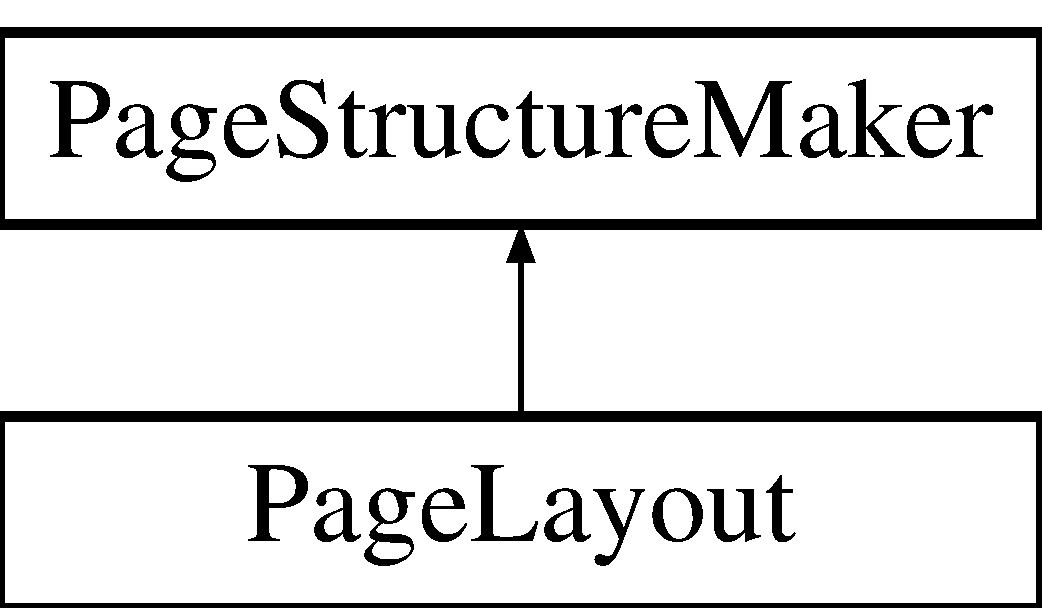
\includegraphics[height=2.000000cm]{classPageStructureMaker}
\end{center}
\end{figure}
\subsection*{Public Member Functions}
\begin{DoxyCompactItemize}
\item 
\hyperlink{classPageStructureMaker_a95e6305a2b5121840fb5b74297a040ce}{Page\-Structure\-Maker} ()
\item 
void \hyperlink{classPageStructureMaker_aaf78d67380c400cc0057c6519276f721}{Set\-H\-T\-M\-L\-Variables} ()
\item 
void \hyperlink{classPageStructureMaker_ad25d6abc983253567e2370882fc1b407}{H\-T\-M\-L\-Start} ()
\item 
void \hyperlink{classPageStructureMaker_a63b877af1c2c8de8332e3f7eb4c2c2b0}{H\-T\-M\-L\-End} ()
\item 
void \hyperlink{classPageStructureMaker_a14312134cb108f91f2e6d9cbd6916e97}{Head\-Start} ()
\item 
void \hyperlink{classPageStructureMaker_ad64115d592b0989b422a93f85278186e}{Head\-End} ()
\item 
void \hyperlink{classPageStructureMaker_a81e902ddc0c0287df1ba0f614a3774d6}{Title} (string page\-Title)
\item 
void \hyperlink{classPageStructureMaker_aacdb11817f8ab246bc59c552e04e862d}{C\-S\-S} (string href)
\item 
void \hyperlink{classPageStructureMaker_ac221d1169f4dbcef6adb00938919193d}{Javascript} (string src)
\item 
void \hyperlink{classPageStructureMaker_ab7a645675166f34fac99f1ed8feb7c27}{Body\-Start} ()
\item 
void \hyperlink{classPageStructureMaker_ac91e234e2d54dedd9d7e556fabf21d2b}{Body\-End} ()
\item 
void \hyperlink{classPageStructureMaker_a927f92889555dd316c129f706be86a5c}{Div\-Start} (string id, string class\-Name)
\item 
void \hyperlink{classPageStructureMaker_a2913e76bf188ed777dcd33003ef6207d}{Div\-End} ()
\item 
void \hyperlink{classPageStructureMaker_a3f25d5b844a2251883acb80d8fabb77d}{Form\-Start} (string name, string action, string method)
\item 
void \hyperlink{classPageStructureMaker_a65d97f23bb543f3db5201b2009f7f65a}{Form\-End} ()
\item 
void \hyperlink{classPageStructureMaker_a04e68e69005f3933e0f496c3db474daf}{Table\-Start} (string id, string class\-Name)
\item 
void \hyperlink{classPageStructureMaker_a7f8fefbe7a825c1b7761fc8a0f1bb8e4}{Table\-End} ()
\item 
void \hyperlink{classPageStructureMaker_ac24ce26202757aaa30402155daf8a3d0}{List\-Start} (string list\-Type)
\item 
void \hyperlink{classPageStructureMaker_a8578b1555ad2fc92a9efc7dbf7d1fe87}{List\-End} (string list\-Type)
\item 
void \hyperlink{classPageStructureMaker_adf4116e526026edc3c8a3bcf96a7e929}{List\-Item} (string list\-Item)
\item 
void \hyperlink{classPageStructureMaker_a8c0fae5b599182863066de56ae0cea42}{Anchor} (string href, string target)
\item 
void \hyperlink{classPageStructureMaker_aec87050d1230402d695290fe78c86f03}{Input\-Field} (string type, string name, string placeholder, string value=\char`\"{}\char`\"{})
\item 
void \hyperlink{classPageStructureMaker_af528f8da142cbc47585c4dfeded873ba}{Input\-Field} (string type, string name, int name\-No, string placeholder, string value=\char`\"{}\char`\"{})
\item 
void \hyperlink{classPageStructureMaker_ae85f66489db9a65682bb9a2c2128f433}{Label} (string for\-Field, string value)
\item 
void \hyperlink{classPageStructureMaker_ae8684bb66ca463e2f92e09c96137f9e3}{Select\-Field\-Start} (string name)
\item 
void \hyperlink{classPageStructureMaker_a81eb3cdbc840a4c8165cef87330ade09}{Select\-Field\-End} ()
\item 
void \hyperlink{classPageStructureMaker_a77856078e74dab25329132ea07466f92}{Select\-Option\-Start} (string value, string selected)
\item 
void \hyperlink{classPageStructureMaker_a7682f479f7f1012d426ec9f9535def60}{Select\-Option\-End} ()
\item 
void \hyperlink{classPageStructureMaker_a53c013b1d6251be853be8f6c413e3455}{Button} (string id, string type, string class\-Name, string value, string on\-Click=\char`\"{}\char`\"{})
\end{DoxyCompactItemize}
\subsection*{Public Attributes}
\begin{DoxyCompactItemize}
\item 
string \hyperlink{classPageStructureMaker_af41d4e21b808f5f8dc2c727f775b6fb2}{start\-H1}
\item 
\hypertarget{classPageStructureMaker_a3786a6f477632e4a60205a988d6b599d}{string {\bfseries end\-H1}}\label{classPageStructureMaker_a3786a6f477632e4a60205a988d6b599d}

\item 
\hypertarget{classPageStructureMaker_adb966c147c6328c8e48281c882de776d}{string {\bfseries start\-H3}}\label{classPageStructureMaker_adb966c147c6328c8e48281c882de776d}

\item 
\hypertarget{classPageStructureMaker_a22e6bf3eb787284b745d694613c1d9da}{string {\bfseries end\-H3}}\label{classPageStructureMaker_a22e6bf3eb787284b745d694613c1d9da}

\item 
\hypertarget{classPageStructureMaker_a7e458e675a3adf987a153e08f3795941}{string {\bfseries start\-T\-D}}\label{classPageStructureMaker_a7e458e675a3adf987a153e08f3795941}

\item 
\hypertarget{classPageStructureMaker_ad27f03939a04048a03be0f1bb8edd38a}{string {\bfseries end\-T\-D}}\label{classPageStructureMaker_ad27f03939a04048a03be0f1bb8edd38a}

\item 
\hypertarget{classPageStructureMaker_a4fe234b016efcb9eaa757879b8858190}{string {\bfseries start\-T\-H}}\label{classPageStructureMaker_a4fe234b016efcb9eaa757879b8858190}

\item 
\hypertarget{classPageStructureMaker_aa244b4ef71850dc76fcfb5157bcaf8fc}{string {\bfseries end\-T\-H}}\label{classPageStructureMaker_aa244b4ef71850dc76fcfb5157bcaf8fc}

\item 
\hypertarget{classPageStructureMaker_aa59b4949d26fab5a72710fa9fc3e8ea9}{string {\bfseries start\-T\-R}}\label{classPageStructureMaker_aa59b4949d26fab5a72710fa9fc3e8ea9}

\item 
\hypertarget{classPageStructureMaker_afee49ebdcbc0971142fcf7eae8baa306}{string {\bfseries end\-T\-R}}\label{classPageStructureMaker_afee49ebdcbc0971142fcf7eae8baa306}

\item 
\hypertarget{classPageStructureMaker_aa0f624b485f07f6e19151b1df3dc59a3}{string {\bfseries start\-B}}\label{classPageStructureMaker_aa0f624b485f07f6e19151b1df3dc59a3}

\item 
\hypertarget{classPageStructureMaker_ad46c3195310a1f0226e21d2eb5befb00}{string {\bfseries end\-B}}\label{classPageStructureMaker_ad46c3195310a1f0226e21d2eb5befb00}

\item 
\hypertarget{classPageStructureMaker_a63911cb925ccdc6c879905a677ed8881}{string {\bfseries brk}}\label{classPageStructureMaker_a63911cb925ccdc6c879905a677ed8881}

\end{DoxyCompactItemize}


\subsection{Detailed Description}
\subsection*{Include Header file }

Class\-: \hyperlink{classPageStructureMaker}{Page\-Structure\-Maker} \subsection*{Description\-: Declaration}

Definition at line 34 of file pagestructure.\-h.



\subsection{Constructor \& Destructor Documentation}
\hypertarget{classPageStructureMaker_a95e6305a2b5121840fb5b74297a040ce}{\index{Page\-Structure\-Maker@{Page\-Structure\-Maker}!Page\-Structure\-Maker@{Page\-Structure\-Maker}}
\index{Page\-Structure\-Maker@{Page\-Structure\-Maker}!PageStructureMaker@{Page\-Structure\-Maker}}
\subsubsection[{Page\-Structure\-Maker}]{\setlength{\rightskip}{0pt plus 5cm}Page\-Structure\-Maker\-::\-Page\-Structure\-Maker (
\begin{DoxyParamCaption}
{}
\end{DoxyParamCaption}
)}}\label{classPageStructureMaker_a95e6305a2b5121840fb5b74297a040ce}
Constructor



 \subsubsection*{Include htmltags.\-h header files}



 Class\-: \hyperlink{classPageStructureMaker}{Page\-Structure\-Maker} Method\-: \hyperlink{classPageStructureMaker}{Page\-Structure\-Maker} \-:\-: \hyperlink{classPageStructureMaker_a95e6305a2b5121840fb5b74297a040ce}{Page\-Structure\-Maker()} \subsubsection*{Description\-: Constructor}

Definition at line 33 of file pagestructure.\-cc.



\subsection{Member Function Documentation}
\hypertarget{classPageStructureMaker_a8c0fae5b599182863066de56ae0cea42}{\index{Page\-Structure\-Maker@{Page\-Structure\-Maker}!Anchor@{Anchor}}
\index{Anchor@{Anchor}!PageStructureMaker@{Page\-Structure\-Maker}}
\subsubsection[{Anchor}]{\setlength{\rightskip}{0pt plus 5cm}void Page\-Structure\-Maker\-::\-Anchor (
\begin{DoxyParamCaption}
\item[{string}]{href, }
\item[{string}]{target}
\end{DoxyParamCaption}
)}}\label{classPageStructureMaker_a8c0fae5b599182863066de56ae0cea42}
Anchor Tag

-\/-\/-\/-\/-\/-\/-\/-\/-\/-\/-\/-\/-\/-\/-\/-\/-\/-\/-\/-\/-\/-\/-\/-\/-\/-\/-\/-\/-\/-\/-\/-\/-\/-\/-\/-\/-\/-\/-\/-\/-\/-\/-\/-\/-\/-\/-\/-\/-\/-\/-\/-\/-\/-\/-\/-\/-\/-\/-\/-\/-\/-\/-\/-\/-\/---\par
 Class\-: \hyperlink{classPageStructureMaker}{Page\-Structure\-Maker} \par
 Method\-: \hyperlink{classPageStructureMaker}{Page\-Structure\-Maker} \-:\-: Anchor(string href) \par
 \subsubsection*{Description\-: Anchor Tag }

Definition at line 319 of file pagestructure.\-cc.

\hypertarget{classPageStructureMaker_ac91e234e2d54dedd9d7e556fabf21d2b}{\index{Page\-Structure\-Maker@{Page\-Structure\-Maker}!Body\-End@{Body\-End}}
\index{Body\-End@{Body\-End}!PageStructureMaker@{Page\-Structure\-Maker}}
\subsubsection[{Body\-End}]{\setlength{\rightskip}{0pt plus 5cm}void Page\-Structure\-Maker\-::\-Body\-End (
\begin{DoxyParamCaption}
{}
\end{DoxyParamCaption}
)}}\label{classPageStructureMaker_ac91e234e2d54dedd9d7e556fabf21d2b}
Display $<$/\-B\-O\-D\-Y$>$



 Class\-: \hyperlink{classPageStructureMaker}{Page\-Structure\-Maker} Method\-: \hyperlink{classPageStructureMaker}{Page\-Structure\-Maker} \-:\-: \hyperlink{classPageStructureMaker_ac91e234e2d54dedd9d7e556fabf21d2b}{Body\-End()} \subsubsection*{Description\-: Display $<$/\-B\-O\-D\-Y$>$}

Definition at line 180 of file pagestructure.\-cc.

\hypertarget{classPageStructureMaker_ab7a645675166f34fac99f1ed8feb7c27}{\index{Page\-Structure\-Maker@{Page\-Structure\-Maker}!Body\-Start@{Body\-Start}}
\index{Body\-Start@{Body\-Start}!PageStructureMaker@{Page\-Structure\-Maker}}
\subsubsection[{Body\-Start}]{\setlength{\rightskip}{0pt plus 5cm}void Page\-Structure\-Maker\-::\-Body\-Start (
\begin{DoxyParamCaption}
{}
\end{DoxyParamCaption}
)}}\label{classPageStructureMaker_ab7a645675166f34fac99f1ed8feb7c27}
Display $<$\-B\-O\-D\-Y$>$



 Class\-: \hyperlink{classPageStructureMaker}{Page\-Structure\-Maker} Method\-: \hyperlink{classPageStructureMaker}{Page\-Structure\-Maker} \-:\-: \hyperlink{classPageStructureMaker_ab7a645675166f34fac99f1ed8feb7c27}{Body\-Start()} \subsubsection*{Description\-: Display $<$B\-O\-D\-Y$>$}

Definition at line 166 of file pagestructure.\-cc.

\hypertarget{classPageStructureMaker_a53c013b1d6251be853be8f6c413e3455}{\index{Page\-Structure\-Maker@{Page\-Structure\-Maker}!Button@{Button}}
\index{Button@{Button}!PageStructureMaker@{Page\-Structure\-Maker}}
\subsubsection[{Button}]{\setlength{\rightskip}{0pt plus 5cm}void Page\-Structure\-Maker\-::\-Button (
\begin{DoxyParamCaption}
\item[{string}]{id, }
\item[{string}]{type, }
\item[{string}]{class\-Name, }
\item[{string}]{value, }
\item[{string}]{on\-Click = {\ttfamily \char`\"{}\char`\"{}}}
\end{DoxyParamCaption}
)}}\label{classPageStructureMaker_a53c013b1d6251be853be8f6c413e3455}
Button



 Class\-: \hyperlink{classPageStructureMaker}{Page\-Structure\-Maker} Method\-: \hyperlink{classPageStructureMaker}{Page\-Structure\-Maker} \-:\-: Button(string id, string type, string class\-Name, string value) \subsubsection*{Description\-: Create button(next, submit, etc)}

Definition at line 474 of file pagestructure.\-cc.

\hypertarget{classPageStructureMaker_aacdb11817f8ab246bc59c552e04e862d}{\index{Page\-Structure\-Maker@{Page\-Structure\-Maker}!C\-S\-S@{C\-S\-S}}
\index{C\-S\-S@{C\-S\-S}!PageStructureMaker@{Page\-Structure\-Maker}}
\subsubsection[{C\-S\-S}]{\setlength{\rightskip}{0pt plus 5cm}void Page\-Structure\-Maker\-::\-C\-S\-S (
\begin{DoxyParamCaption}
\item[{string}]{href}
\end{DoxyParamCaption}
)}}\label{classPageStructureMaker_aacdb11817f8ab246bc59c552e04e862d}
Add External C\-S\-S



 Class\-: \hyperlink{classPageStructureMaker}{Page\-Structure\-Maker} Method\-: \hyperlink{classPageStructureMaker}{Page\-Structure\-Maker} \-:\-: \hyperlink{classPageStructureMaker_aacdb11817f8ab246bc59c552e04e862d}{C\-S\-S(string href)} \subsubsection*{Description\-: Add External C\-S\-S file}

Definition at line 138 of file pagestructure.\-cc.

\hypertarget{classPageStructureMaker_a2913e76bf188ed777dcd33003ef6207d}{\index{Page\-Structure\-Maker@{Page\-Structure\-Maker}!Div\-End@{Div\-End}}
\index{Div\-End@{Div\-End}!PageStructureMaker@{Page\-Structure\-Maker}}
\subsubsection[{Div\-End}]{\setlength{\rightskip}{0pt plus 5cm}void Page\-Structure\-Maker\-::\-Div\-End (
\begin{DoxyParamCaption}
{}
\end{DoxyParamCaption}
)}}\label{classPageStructureMaker_a2913e76bf188ed777dcd33003ef6207d}
End div section



 Class\-: \hyperlink{classPageStructureMaker}{Page\-Structure\-Maker} Method\-: \hyperlink{classPageStructureMaker}{Page\-Structure\-Maker} \-:\-: \hyperlink{classPageStructureMaker_a2913e76bf188ed777dcd33003ef6207d}{Div\-End()} \subsubsection*{Description\-: Close Div Section}

Definition at line 209 of file pagestructure.\-cc.

\hypertarget{classPageStructureMaker_a927f92889555dd316c129f706be86a5c}{\index{Page\-Structure\-Maker@{Page\-Structure\-Maker}!Div\-Start@{Div\-Start}}
\index{Div\-Start@{Div\-Start}!PageStructureMaker@{Page\-Structure\-Maker}}
\subsubsection[{Div\-Start}]{\setlength{\rightskip}{0pt plus 5cm}void Page\-Structure\-Maker\-::\-Div\-Start (
\begin{DoxyParamCaption}
\item[{string}]{id, }
\item[{string}]{class\-Name}
\end{DoxyParamCaption}
)}}\label{classPageStructureMaker_a927f92889555dd316c129f706be86a5c}
Start Div Section



 Class\-: \hyperlink{classPageStructureMaker}{Page\-Structure\-Maker} Method\-: \hyperlink{classPageStructureMaker}{Page\-Structure\-Maker} \-:\-: Div\-Start(string id, string class\-Name) \subsubsection*{Description\-: Start Div Section with id and class\-Name(for C\-S\-S)}

Definition at line 195 of file pagestructure.\-cc.

\hypertarget{classPageStructureMaker_a65d97f23bb543f3db5201b2009f7f65a}{\index{Page\-Structure\-Maker@{Page\-Structure\-Maker}!Form\-End@{Form\-End}}
\index{Form\-End@{Form\-End}!PageStructureMaker@{Page\-Structure\-Maker}}
\subsubsection[{Form\-End}]{\setlength{\rightskip}{0pt plus 5cm}void Page\-Structure\-Maker\-::\-Form\-End (
\begin{DoxyParamCaption}
{}
\end{DoxyParamCaption}
)}}\label{classPageStructureMaker_a65d97f23bb543f3db5201b2009f7f65a}
End Form



 Class\-: \hyperlink{classPageStructureMaker}{Page\-Structure\-Maker} Method\-: \hyperlink{classPageStructureMaker}{Page\-Structure\-Maker} \-:\-: \hyperlink{classPageStructureMaker_a65d97f23bb543f3db5201b2009f7f65a}{Form\-End()} \subsubsection*{Description\-: Close Form}

Definition at line 239 of file pagestructure.\-cc.

\hypertarget{classPageStructureMaker_a3f25d5b844a2251883acb80d8fabb77d}{\index{Page\-Structure\-Maker@{Page\-Structure\-Maker}!Form\-Start@{Form\-Start}}
\index{Form\-Start@{Form\-Start}!PageStructureMaker@{Page\-Structure\-Maker}}
\subsubsection[{Form\-Start}]{\setlength{\rightskip}{0pt plus 5cm}void Page\-Structure\-Maker\-::\-Form\-Start (
\begin{DoxyParamCaption}
\item[{string}]{name, }
\item[{string}]{action, }
\item[{string}]{method}
\end{DoxyParamCaption}
)}}\label{classPageStructureMaker_a3f25d5b844a2251883acb80d8fabb77d}
Start Form



 Class\-: \hyperlink{classPageStructureMaker}{Page\-Structure\-Maker} Method\-: \hyperlink{classPageStructureMaker}{Page\-Structure\-Maker} \-:\-: Form\-Start(string name, string action, string method) \subsubsection*{Description\-: Start Form with name, action and method(G\-E\-T/\-P\-O\-S\-T)}

Definition at line 223 of file pagestructure.\-cc.

\hypertarget{classPageStructureMaker_ad64115d592b0989b422a93f85278186e}{\index{Page\-Structure\-Maker@{Page\-Structure\-Maker}!Head\-End@{Head\-End}}
\index{Head\-End@{Head\-End}!PageStructureMaker@{Page\-Structure\-Maker}}
\subsubsection[{Head\-End}]{\setlength{\rightskip}{0pt plus 5cm}void Page\-Structure\-Maker\-::\-Head\-End (
\begin{DoxyParamCaption}
{}
\end{DoxyParamCaption}
)}}\label{classPageStructureMaker_ad64115d592b0989b422a93f85278186e}
Display $<$/\-H\-E\-A\-D$>$



 Class\-: \hyperlink{classPageStructureMaker}{Page\-Structure\-Maker} Method\-: \hyperlink{classPageStructureMaker}{Page\-Structure\-Maker} \-:\-: \hyperlink{classPageStructureMaker_ad64115d592b0989b422a93f85278186e}{Head\-End()} \subsubsection*{Description\-: Display $<$/\-H\-E\-A\-D$>$}

Definition at line 112 of file pagestructure.\-cc.

\hypertarget{classPageStructureMaker_a14312134cb108f91f2e6d9cbd6916e97}{\index{Page\-Structure\-Maker@{Page\-Structure\-Maker}!Head\-Start@{Head\-Start}}
\index{Head\-Start@{Head\-Start}!PageStructureMaker@{Page\-Structure\-Maker}}
\subsubsection[{Head\-Start}]{\setlength{\rightskip}{0pt plus 5cm}void Page\-Structure\-Maker\-::\-Head\-Start (
\begin{DoxyParamCaption}
{}
\end{DoxyParamCaption}
)}}\label{classPageStructureMaker_a14312134cb108f91f2e6d9cbd6916e97}
Display $<$\-H\-E\-A\-D$>$



 Class\-: \hyperlink{classPageStructureMaker}{Page\-Structure\-Maker} Method\-: \hyperlink{classPageStructureMaker}{Page\-Structure\-Maker} \-:\-: \hyperlink{classPageStructureMaker_a14312134cb108f91f2e6d9cbd6916e97}{Head\-Start()} \subsubsection*{Description\-: Display $<$H\-E\-A\-D$>$}

Definition at line 99 of file pagestructure.\-cc.

\hypertarget{classPageStructureMaker_a63b877af1c2c8de8332e3f7eb4c2c2b0}{\index{Page\-Structure\-Maker@{Page\-Structure\-Maker}!H\-T\-M\-L\-End@{H\-T\-M\-L\-End}}
\index{H\-T\-M\-L\-End@{H\-T\-M\-L\-End}!PageStructureMaker@{Page\-Structure\-Maker}}
\subsubsection[{H\-T\-M\-L\-End}]{\setlength{\rightskip}{0pt plus 5cm}void Page\-Structure\-Maker\-::\-H\-T\-M\-L\-End (
\begin{DoxyParamCaption}
{}
\end{DoxyParamCaption}
)}}\label{classPageStructureMaker_a63b877af1c2c8de8332e3f7eb4c2c2b0}
Display $<$/\-H\-T\-M\-L$>$



 Class\-: \hyperlink{classPageStructureMaker}{Page\-Structure\-Maker} Method\-: \hyperlink{classPageStructureMaker}{Page\-Structure\-Maker} \-:\-: \hyperlink{classPageStructureMaker_a63b877af1c2c8de8332e3f7eb4c2c2b0}{H\-T\-M\-L\-End()} \subsubsection*{Description\-: Display $<$/\-H\-T\-M\-L$>$}

Definition at line 86 of file pagestructure.\-cc.

\hypertarget{classPageStructureMaker_ad25d6abc983253567e2370882fc1b407}{\index{Page\-Structure\-Maker@{Page\-Structure\-Maker}!H\-T\-M\-L\-Start@{H\-T\-M\-L\-Start}}
\index{H\-T\-M\-L\-Start@{H\-T\-M\-L\-Start}!PageStructureMaker@{Page\-Structure\-Maker}}
\subsubsection[{H\-T\-M\-L\-Start}]{\setlength{\rightskip}{0pt plus 5cm}void Page\-Structure\-Maker\-::\-H\-T\-M\-L\-Start (
\begin{DoxyParamCaption}
{}
\end{DoxyParamCaption}
)}}\label{classPageStructureMaker_ad25d6abc983253567e2370882fc1b407}
Display $<$\-H\-T\-M\-L$>$



 Class\-: \hyperlink{classPageStructureMaker}{Page\-Structure\-Maker} Method\-: \hyperlink{classPageStructureMaker}{Page\-Structure\-Maker} \-:\-: \hyperlink{classPageStructureMaker_ad25d6abc983253567e2370882fc1b407}{H\-T\-M\-L\-Start()} \subsubsection*{Description\-: Display $<$H\-T\-M\-L$>$ Tag }

Definition at line 73 of file pagestructure.\-cc.

\hypertarget{classPageStructureMaker_aec87050d1230402d695290fe78c86f03}{\index{Page\-Structure\-Maker@{Page\-Structure\-Maker}!Input\-Field@{Input\-Field}}
\index{Input\-Field@{Input\-Field}!PageStructureMaker@{Page\-Structure\-Maker}}
\subsubsection[{Input\-Field}]{\setlength{\rightskip}{0pt plus 5cm}void Page\-Structure\-Maker\-::\-Input\-Field (
\begin{DoxyParamCaption}
\item[{string}]{type, }
\item[{string}]{name, }
\item[{string}]{placeholder, }
\item[{string}]{value = {\ttfamily \char`\"{}\char`\"{}}}
\end{DoxyParamCaption}
)}}\label{classPageStructureMaker_aec87050d1230402d695290fe78c86f03}
Input field with 3 arguments

-\/-\/-\/-\/-\/-\/-\/-\/-\/-\/-\/-\/-\/-\/-\/-\/-\/-\/-\/-\/-\/-\/-\/-\/-\/-\/-\/-\/-\/-\/-\/-\/-\/-\/-\/-\/-\/-\/-\/-\/-\/-\/-\/-\/-\/-\/-\/-\/-\/-\/-\/-\/-\/-\/-\/-\/-\/-\/-\/-\/-\/-\/-\/-\/-\/---\par
 Class\-: \hyperlink{classPageStructureMaker}{Page\-Structure\-Maker} \par
 Method\-: \hyperlink{classPageStructureMaker}{Page\-Structure\-Maker} \-:\-: Input\-Field(string type, string name, string value) \par
 \subsubsection*{Description\-: For creating input field with 3 arguments }

Definition at line 348 of file pagestructure.\-cc.

\hypertarget{classPageStructureMaker_af528f8da142cbc47585c4dfeded873ba}{\index{Page\-Structure\-Maker@{Page\-Structure\-Maker}!Input\-Field@{Input\-Field}}
\index{Input\-Field@{Input\-Field}!PageStructureMaker@{Page\-Structure\-Maker}}
\subsubsection[{Input\-Field}]{\setlength{\rightskip}{0pt plus 5cm}void Page\-Structure\-Maker\-::\-Input\-Field (
\begin{DoxyParamCaption}
\item[{string}]{type, }
\item[{string}]{name, }
\item[{int}]{name\-No, }
\item[{string}]{placeholder, }
\item[{string}]{value = {\ttfamily \char`\"{}\char`\"{}}}
\end{DoxyParamCaption}
)}}\label{classPageStructureMaker_af528f8da142cbc47585c4dfeded873ba}
Input Field with 4 arguments



 Class\-: \hyperlink{classPageStructureMaker}{Page\-Structure\-Maker} Method\-: \hyperlink{classPageStructureMaker}{Page\-Structure\-Maker} \-:\-: Input\-Field(string type, string name, string value) Description\-: Create Input fields like text field, submit \subsubsection*{button, etc.}

Definition at line 386 of file pagestructure.\-cc.

\hypertarget{classPageStructureMaker_ac221d1169f4dbcef6adb00938919193d}{\index{Page\-Structure\-Maker@{Page\-Structure\-Maker}!Javascript@{Javascript}}
\index{Javascript@{Javascript}!PageStructureMaker@{Page\-Structure\-Maker}}
\subsubsection[{Javascript}]{\setlength{\rightskip}{0pt plus 5cm}void Page\-Structure\-Maker\-::\-Javascript (
\begin{DoxyParamCaption}
\item[{string}]{src}
\end{DoxyParamCaption}
)}}\label{classPageStructureMaker_ac221d1169f4dbcef6adb00938919193d}
Add Javascript File



 Class\-: \hyperlink{classPageStructureMaker}{Page\-Structure\-Maker} Method\-: \hyperlink{classPageStructureMaker}{Page\-Structure\-Maker} \-:\-: \hyperlink{classPageStructureMaker_ac221d1169f4dbcef6adb00938919193d}{Javascript(string src)} \subsubsection*{Description\-: Add external Javascript file}

Definition at line 153 of file pagestructure.\-cc.

\hypertarget{classPageStructureMaker_ae85f66489db9a65682bb9a2c2128f433}{\index{Page\-Structure\-Maker@{Page\-Structure\-Maker}!Label@{Label}}
\index{Label@{Label}!PageStructureMaker@{Page\-Structure\-Maker}}
\subsubsection[{Label}]{\setlength{\rightskip}{0pt plus 5cm}void Page\-Structure\-Maker\-::\-Label (
\begin{DoxyParamCaption}
\item[{string}]{for\-Field, }
\item[{string}]{value}
\end{DoxyParamCaption}
)}}\label{classPageStructureMaker_ae85f66489db9a65682bb9a2c2128f433}
Label tag

-\/-\/-\/-\/-\/-\/-\/-\/-\/-\/-\/-\/-\/-\/-\/-\/-\/-\/-\/-\/-\/-\/-\/-\/-\/-\/-\/-\/-\/-\/-\/-\/-\/-\/-\/-\/-\/-\/-\/-\/-\/-\/-\/-\/-\/-\/-\/-\/-\/-\/-\/-\/-\/-\/-\/-\/-\/-\/-\/-\/-\/-\/-\/-\/-\/---\par
 Class\-: \hyperlink{classPageStructureMaker}{Page\-Structure\-Maker} \par
 Method\-: \hyperlink{classPageStructureMaker}{Page\-Structure\-Maker} \-:\-: Label(string for\-Value, string value) \par
 \subsubsection*{Description\-: For adding label in html page }

Definition at line 333 of file pagestructure.\-cc.

\hypertarget{classPageStructureMaker_a8578b1555ad2fc92a9efc7dbf7d1fe87}{\index{Page\-Structure\-Maker@{Page\-Structure\-Maker}!List\-End@{List\-End}}
\index{List\-End@{List\-End}!PageStructureMaker@{Page\-Structure\-Maker}}
\subsubsection[{List\-End}]{\setlength{\rightskip}{0pt plus 5cm}void Page\-Structure\-Maker\-::\-List\-End (
\begin{DoxyParamCaption}
\item[{string}]{list\-Type}
\end{DoxyParamCaption}
)}}\label{classPageStructureMaker_a8578b1555ad2fc92a9efc7dbf7d1fe87}
End List

-\/-\/-\/-\/-\/-\/-\/-\/-\/-\/-\/-\/-\/-\/-\/-\/-\/-\/-\/-\/-\/-\/-\/-\/-\/-\/-\/-\/-\/-\/-\/-\/-\/-\/-\/-\/-\/-\/-\/-\/-\/-\/-\/-\/-\/-\/-\/-\/-\/-\/-\/-\/-\/-\/-\/-\/-\/-\/-\/-\/-\/-\/-\/-\/-\/---\par
 Class\-: \hyperlink{classPageStructureMaker}{Page\-Structure\-Maker} \par
 Method\-: \hyperlink{classPageStructureMaker}{Page\-Structure\-Maker} \-:\-: \hyperlink{classPageStructureMaker_a8578b1555ad2fc92a9efc7dbf7d1fe87}{List\-End(string list\-Type)} \par
 \subsubsection*{Description\-: Close List Tag }

Definition at line 293 of file pagestructure.\-cc.

\hypertarget{classPageStructureMaker_adf4116e526026edc3c8a3bcf96a7e929}{\index{Page\-Structure\-Maker@{Page\-Structure\-Maker}!List\-Item@{List\-Item}}
\index{List\-Item@{List\-Item}!PageStructureMaker@{Page\-Structure\-Maker}}
\subsubsection[{List\-Item}]{\setlength{\rightskip}{0pt plus 5cm}void Page\-Structure\-Maker\-::\-List\-Item (
\begin{DoxyParamCaption}
\item[{string}]{list\-Item}
\end{DoxyParamCaption}
)}}\label{classPageStructureMaker_adf4116e526026edc3c8a3bcf96a7e929}
List Item

-\/-\/-\/-\/-\/-\/-\/-\/-\/-\/-\/-\/-\/-\/-\/-\/-\/-\/-\/-\/-\/-\/-\/-\/-\/-\/-\/-\/-\/-\/-\/-\/-\/-\/-\/-\/-\/-\/-\/-\/-\/-\/-\/-\/-\/-\/-\/-\/-\/-\/-\/-\/-\/-\/-\/-\/-\/-\/-\/-\/-\/-\/-\/-\/-\/---\par
 Class\-: \hyperlink{classPageStructureMaker}{Page\-Structure\-Maker} \par
 Method\-: \hyperlink{classPageStructureMaker}{Page\-Structure\-Maker} \-:\-: \hyperlink{classPageStructureMaker_adf4116e526026edc3c8a3bcf96a7e929}{List\-Item(string list\-Item)} \par
 \subsubsection*{Description\-: List Item }

Definition at line 306 of file pagestructure.\-cc.

\hypertarget{classPageStructureMaker_ac24ce26202757aaa30402155daf8a3d0}{\index{Page\-Structure\-Maker@{Page\-Structure\-Maker}!List\-Start@{List\-Start}}
\index{List\-Start@{List\-Start}!PageStructureMaker@{Page\-Structure\-Maker}}
\subsubsection[{List\-Start}]{\setlength{\rightskip}{0pt plus 5cm}void Page\-Structure\-Maker\-::\-List\-Start (
\begin{DoxyParamCaption}
\item[{string}]{list\-Type}
\end{DoxyParamCaption}
)}}\label{classPageStructureMaker_ac24ce26202757aaa30402155daf8a3d0}
Start List

-\/-\/-\/-\/-\/-\/-\/-\/-\/-\/-\/-\/-\/-\/-\/-\/-\/-\/-\/-\/-\/-\/-\/-\/-\/-\/-\/-\/-\/-\/-\/-\/-\/-\/-\/-\/-\/-\/-\/-\/-\/-\/-\/-\/-\/-\/-\/-\/-\/-\/-\/-\/-\/-\/-\/-\/-\/-\/-\/-\/-\/-\/-\/-\/-\/---\par
 Class\-: \hyperlink{classPageStructureMaker}{Page\-Structure\-Maker} \par
 Method\-: \hyperlink{classPageStructureMaker}{Page\-Structure\-Maker} \-:\-: \hyperlink{classPageStructureMaker_ac24ce26202757aaa30402155daf8a3d0}{List\-Start(string list\-Type)} \par
 \subsubsection*{Description\-: Start any list like ul, ol, etc. }

Definition at line 280 of file pagestructure.\-cc.

\hypertarget{classPageStructureMaker_a81eb3cdbc840a4c8165cef87330ade09}{\index{Page\-Structure\-Maker@{Page\-Structure\-Maker}!Select\-Field\-End@{Select\-Field\-End}}
\index{Select\-Field\-End@{Select\-Field\-End}!PageStructureMaker@{Page\-Structure\-Maker}}
\subsubsection[{Select\-Field\-End}]{\setlength{\rightskip}{0pt plus 5cm}void Page\-Structure\-Maker\-::\-Select\-Field\-End (
\begin{DoxyParamCaption}
{}
\end{DoxyParamCaption}
)}}\label{classPageStructureMaker_a81eb3cdbc840a4c8165cef87330ade09}
End Select Field



 Class\-: \hyperlink{classPageStructureMaker}{Page\-Structure\-Maker} Method\-: \hyperlink{classPageStructureMaker}{Page\-Structure\-Maker} \-:\-: \hyperlink{classPageStructureMaker_a81eb3cdbc840a4c8165cef87330ade09}{Select\-Field\-End()} \subsubsection*{Description\-: Close select field}

Definition at line 430 of file pagestructure.\-cc.

\hypertarget{classPageStructureMaker_ae8684bb66ca463e2f92e09c96137f9e3}{\index{Page\-Structure\-Maker@{Page\-Structure\-Maker}!Select\-Field\-Start@{Select\-Field\-Start}}
\index{Select\-Field\-Start@{Select\-Field\-Start}!PageStructureMaker@{Page\-Structure\-Maker}}
\subsubsection[{Select\-Field\-Start}]{\setlength{\rightskip}{0pt plus 5cm}void Page\-Structure\-Maker\-::\-Select\-Field\-Start (
\begin{DoxyParamCaption}
\item[{string}]{name}
\end{DoxyParamCaption}
)}}\label{classPageStructureMaker_ae8684bb66ca463e2f92e09c96137f9e3}
Select Field Start



 Class\-: \hyperlink{classPageStructureMaker}{Page\-Structure\-Maker} Method\-: \hyperlink{classPageStructureMaker}{Page\-Structure\-Maker} \-:\-: \hyperlink{classPageStructureMaker_ae8684bb66ca463e2f92e09c96137f9e3}{Select\-Field\-Start(string name)} \subsubsection*{Description\-: Create Select Field}

Definition at line 417 of file pagestructure.\-cc.

\hypertarget{classPageStructureMaker_a7682f479f7f1012d426ec9f9535def60}{\index{Page\-Structure\-Maker@{Page\-Structure\-Maker}!Select\-Option\-End@{Select\-Option\-End}}
\index{Select\-Option\-End@{Select\-Option\-End}!PageStructureMaker@{Page\-Structure\-Maker}}
\subsubsection[{Select\-Option\-End}]{\setlength{\rightskip}{0pt plus 5cm}void Page\-Structure\-Maker\-::\-Select\-Option\-End (
\begin{DoxyParamCaption}
{}
\end{DoxyParamCaption}
)}}\label{classPageStructureMaker_a7682f479f7f1012d426ec9f9535def60}
Selct Option End



 Class\-: \hyperlink{classPageStructureMaker}{Page\-Structure\-Maker} Method\-: \hyperlink{classPageStructureMaker}{Page\-Structure\-Maker} \-:\-: \hyperlink{classPageStructureMaker_a7682f479f7f1012d426ec9f9535def60}{Select\-Option\-End()} \subsubsection*{Description\-: Close select option}

Definition at line 460 of file pagestructure.\-cc.

\hypertarget{classPageStructureMaker_a77856078e74dab25329132ea07466f92}{\index{Page\-Structure\-Maker@{Page\-Structure\-Maker}!Select\-Option\-Start@{Select\-Option\-Start}}
\index{Select\-Option\-Start@{Select\-Option\-Start}!PageStructureMaker@{Page\-Structure\-Maker}}
\subsubsection[{Select\-Option\-Start}]{\setlength{\rightskip}{0pt plus 5cm}void Page\-Structure\-Maker\-::\-Select\-Option\-Start (
\begin{DoxyParamCaption}
\item[{string}]{value, }
\item[{string}]{selected}
\end{DoxyParamCaption}
)}}\label{classPageStructureMaker_a77856078e74dab25329132ea07466f92}
Select Option Start



 Class\-: \hyperlink{classPageStructureMaker}{Page\-Structure\-Maker} Method\-: \hyperlink{classPageStructureMaker}{Page\-Structure\-Maker} \-:\-: Select\-Option\-Start(string value, string selected) \subsubsection*{Description\-: Options for select }

Definition at line 444 of file pagestructure.\-cc.

\hypertarget{classPageStructureMaker_aaf78d67380c400cc0057c6519276f721}{\index{Page\-Structure\-Maker@{Page\-Structure\-Maker}!Set\-H\-T\-M\-L\-Variables@{Set\-H\-T\-M\-L\-Variables}}
\index{Set\-H\-T\-M\-L\-Variables@{Set\-H\-T\-M\-L\-Variables}!PageStructureMaker@{Page\-Structure\-Maker}}
\subsubsection[{Set\-H\-T\-M\-L\-Variables}]{\setlength{\rightskip}{0pt plus 5cm}void Page\-Structure\-Maker\-::\-Set\-H\-T\-M\-L\-Variables (
\begin{DoxyParamCaption}
{}
\end{DoxyParamCaption}
)}}\label{classPageStructureMaker_aaf78d67380c400cc0057c6519276f721}
Assingn Values to variables



 Class\-: \hyperlink{classPageStructureMaker}{Page\-Structure\-Maker} Method\-: \hyperlink{classPageStructureMaker}{Page\-Structure\-Maker} \-:\-: \hyperlink{classPageStructureMaker_aaf78d67380c400cc0057c6519276f721}{Set\-H\-T\-M\-L\-Variables()} Description\-: Set values of common H\-T\-M\-L tags in respective \subsubsection*{variables.}

Definition at line 48 of file pagestructure.\-cc.

\hypertarget{classPageStructureMaker_a7f8fefbe7a825c1b7761fc8a0f1bb8e4}{\index{Page\-Structure\-Maker@{Page\-Structure\-Maker}!Table\-End@{Table\-End}}
\index{Table\-End@{Table\-End}!PageStructureMaker@{Page\-Structure\-Maker}}
\subsubsection[{Table\-End}]{\setlength{\rightskip}{0pt plus 5cm}void Page\-Structure\-Maker\-::\-Table\-End (
\begin{DoxyParamCaption}
{}
\end{DoxyParamCaption}
)}}\label{classPageStructureMaker_a7f8fefbe7a825c1b7761fc8a0f1bb8e4}
End Table



 Class\-: \hyperlink{classPageStructureMaker}{Page\-Structure\-Maker} Method\-: \hyperlink{classPageStructureMaker}{Page\-Structure\-Maker} \-:\-: \hyperlink{classPageStructureMaker_a7f8fefbe7a825c1b7761fc8a0f1bb8e4}{Table\-End()} \subsubsection*{Description\-: Close Table tag}

Definition at line 267 of file pagestructure.\-cc.

\hypertarget{classPageStructureMaker_a04e68e69005f3933e0f496c3db474daf}{\index{Page\-Structure\-Maker@{Page\-Structure\-Maker}!Table\-Start@{Table\-Start}}
\index{Table\-Start@{Table\-Start}!PageStructureMaker@{Page\-Structure\-Maker}}
\subsubsection[{Table\-Start}]{\setlength{\rightskip}{0pt plus 5cm}void Page\-Structure\-Maker\-::\-Table\-Start (
\begin{DoxyParamCaption}
\item[{string}]{id, }
\item[{string}]{class\-Name}
\end{DoxyParamCaption}
)}}\label{classPageStructureMaker_a04e68e69005f3933e0f496c3db474daf}
Start Table



 Class\-: \hyperlink{classPageStructureMaker}{Page\-Structure\-Maker} Method\-: \hyperlink{classPageStructureMaker}{Page\-Structure\-Maker} \-:\-: Table\-Start(string id, string class\-Name) \subsubsection*{Description\-: Start Table with id and class\-Name(\-C\-S\-S) attributes}

Definition at line 253 of file pagestructure.\-cc.

\hypertarget{classPageStructureMaker_a81e902ddc0c0287df1ba0f614a3774d6}{\index{Page\-Structure\-Maker@{Page\-Structure\-Maker}!Title@{Title}}
\index{Title@{Title}!PageStructureMaker@{Page\-Structure\-Maker}}
\subsubsection[{Title}]{\setlength{\rightskip}{0pt plus 5cm}void Page\-Structure\-Maker\-::\-Title (
\begin{DoxyParamCaption}
\item[{string}]{page\-Title}
\end{DoxyParamCaption}
)}}\label{classPageStructureMaker_a81e902ddc0c0287df1ba0f614a3774d6}
Display $<$\-T\-I\-T\-L\-E$>$ $<$/\-T\-I\-T\-L\-E$>$



 Class\-: \hyperlink{classPageStructureMaker}{Page\-Structure\-Maker} Method\-: \hyperlink{classPageStructureMaker}{Page\-Structure\-Maker} \-:\-: \hyperlink{classPageStructureMaker_a81e902ddc0c0287df1ba0f614a3774d6}{Title(string page\-Title)} \subsubsection*{Description\-: Display Page Tile}

Definition at line 125 of file pagestructure.\-cc.



\subsection{Member Data Documentation}
\hypertarget{classPageStructureMaker_af41d4e21b808f5f8dc2c727f775b6fb2}{\index{Page\-Structure\-Maker@{Page\-Structure\-Maker}!start\-H1@{start\-H1}}
\index{start\-H1@{start\-H1}!PageStructureMaker@{Page\-Structure\-Maker}}
\subsubsection[{start\-H1}]{\setlength{\rightskip}{0pt plus 5cm}string Page\-Structure\-Maker\-::start\-H1}}\label{classPageStructureMaker_af41d4e21b808f5f8dc2c727f775b6fb2}
H\-T\-M\-L Tag Variables for td, th, bold, etc 

Definition at line 38 of file pagestructure.\-h.



The documentation for this class was generated from the following files\-:\begin{DoxyCompactItemize}
\item 
src/header/pagestructure.\-h\item 
src/pagestructure.\-cc\end{DoxyCompactItemize}

\hypertarget{classProjectDetail}{\section{Project\-Detail Class Reference}
\label{classProjectDetail}\index{Project\-Detail@{Project\-Detail}}
}


\hyperlink{classProjectDetail}{Project\-Detail} class for creating new project for user.  




{\ttfamily \#include $<$project.\-h$>$}

Inheritance diagram for Project\-Detail\-:\begin{figure}[H]
\begin{center}
\leavevmode
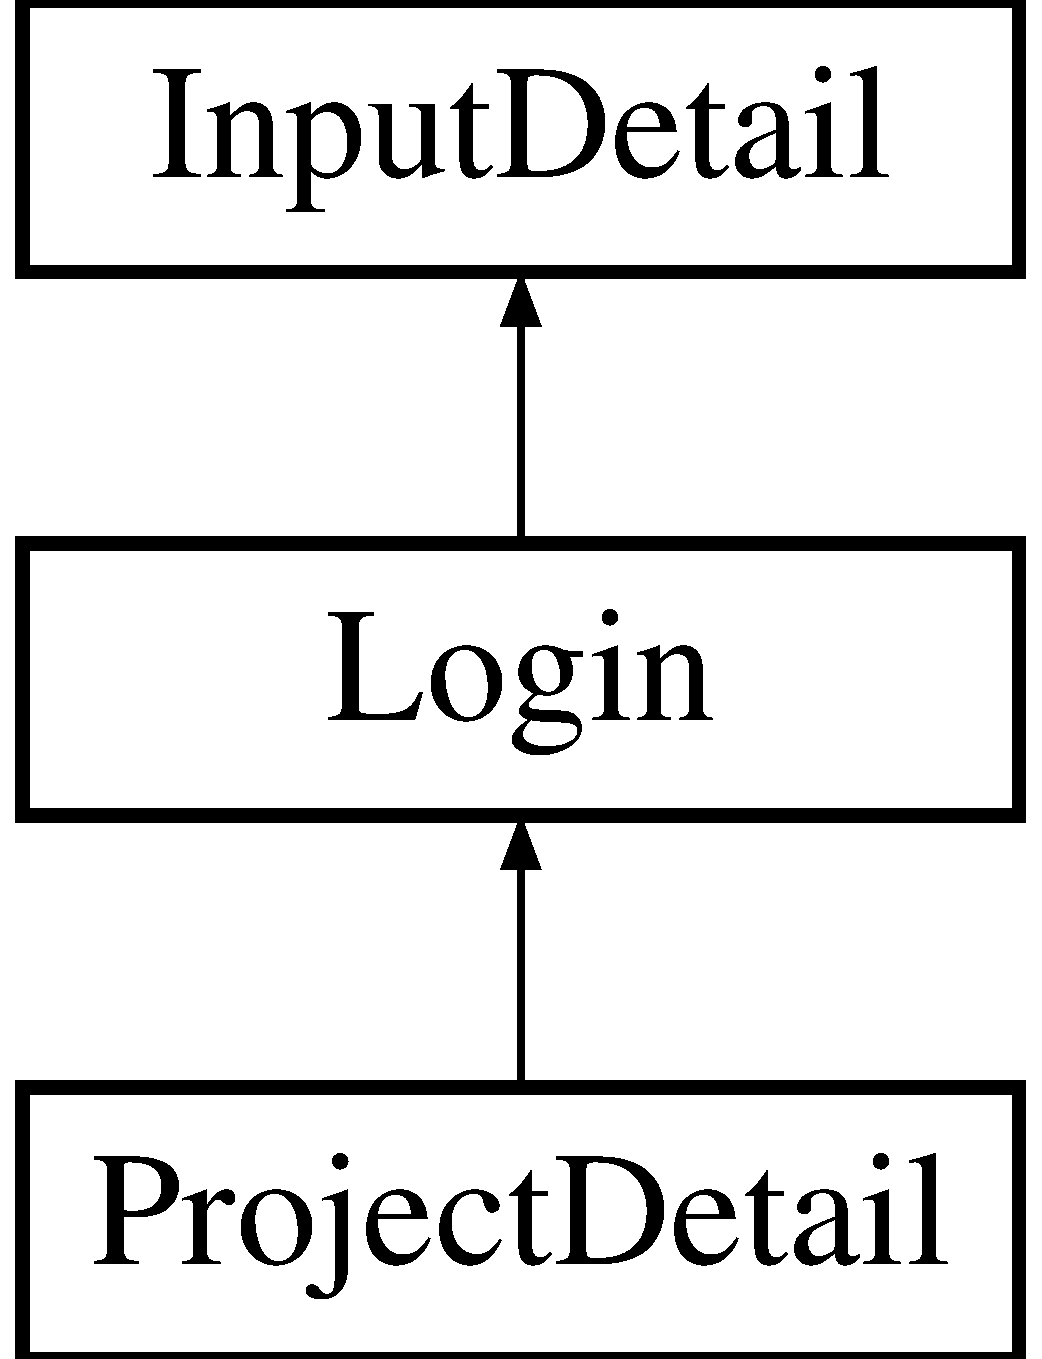
\includegraphics[height=3.000000cm]{classProjectDetail}
\end{center}
\end{figure}
\subsection*{Public Member Functions}
\begin{DoxyCompactItemize}
\item 
\hyperlink{classProjectDetail_a405e8bbc157e30c4ff93871988218d9f}{Project\-Detail} ()
\item 
void \hyperlink{classProjectDetail_a581ccdab5dcd21663b78ebedbbf0d240}{Project\-Detail\-Page} (string \hyperlink{classInputDetail_a1abb16cd695678c3fa05e3c812823fee}{msg}=\char`\"{}\char`\"{}, string project\-Name=\char`\"{}Project Name\char`\"{})
\item 
void \hyperlink{classProjectDetail_ab78c9e2a0cd5079c427638a5a3971c28}{Authorize\-User} ()
\item 
\hypertarget{classProjectDetail_ab92c992a37524a5f90fdcaf4868ac218}{void \hyperlink{classProjectDetail_ab92c992a37524a5f90fdcaf4868ac218}{Old\-Project} ()}\label{classProjectDetail_ab92c992a37524a5f90fdcaf4868ac218}

\begin{DoxyCompactList}\small\item\em List Existing projects from database. \end{DoxyCompactList}\item 
\hypertarget{classProjectDetail_aa36fe7134da17688018870ae8ebf2191}{void \hyperlink{classProjectDetail_aa36fe7134da17688018870ae8ebf2191}{Home\-Page} ()}\label{classProjectDetail_aa36fe7134da17688018870ae8ebf2191}

\begin{DoxyCompactList}\small\item\em Home Page. \end{DoxyCompactList}\item 
\hyperlink{classProjectDetail_ab4719d14d9efb8811916f5d691099c8f}{$\sim$\-Project\-Detail} ()
\end{DoxyCompactItemize}
\subsection*{Additional Inherited Members}


\subsection{Detailed Description}
\hyperlink{classProjectDetail}{Project\-Detail} class for creating new project for user. 

Definition at line 28 of file project.\-h.



\subsection{Constructor \& Destructor Documentation}
\hypertarget{classProjectDetail_a405e8bbc157e30c4ff93871988218d9f}{\index{Project\-Detail@{Project\-Detail}!Project\-Detail@{Project\-Detail}}
\index{Project\-Detail@{Project\-Detail}!ProjectDetail@{Project\-Detail}}
\subsubsection[{Project\-Detail}]{\setlength{\rightskip}{0pt plus 5cm}Project\-Detail\-::\-Project\-Detail (
\begin{DoxyParamCaption}
{}
\end{DoxyParamCaption}
)}}\label{classProjectDetail_a405e8bbc157e30c4ff93871988218d9f}
include projectdetail.\-h -\/-\/-\/-\/-\/-\/-\/-\/-\/-\/-\/-\/-\/-\/-\/-\/-\/-\/-\/-\/-\/-\/-\/-\/-\/-\/-\/-\/-\/-\/-\/-\/-\/-\/-\/-\/-\/-\/-\/-\/-\/-\/-\/-\/-\/-\/-\/-\/-\/-\/-\/-\/-\/-\/-\/-\/-\/-\/-\/-\/-\/-\/-\/-\/-\/---\par
 Class\-: \hyperlink{classProjectDetail}{Project\-Detail} \par
 Method\-: \hyperlink{classProjectDetail}{Project\-Detail} \-:\-: \hyperlink{classProjectDetail_a405e8bbc157e30c4ff93871988218d9f}{Project\-Detail()} \par
\subsubsection*{Description\-: Constructor of \hyperlink{classProjectDetail}{Project\-Detail} }

Definition at line 29 of file project.\-cc.

\hypertarget{classProjectDetail_ab4719d14d9efb8811916f5d691099c8f}{\index{Project\-Detail@{Project\-Detail}!$\sim$\-Project\-Detail@{$\sim$\-Project\-Detail}}
\index{$\sim$\-Project\-Detail@{$\sim$\-Project\-Detail}!ProjectDetail@{Project\-Detail}}
\subsubsection[{$\sim$\-Project\-Detail}]{\setlength{\rightskip}{0pt plus 5cm}Project\-Detail\-::$\sim$\-Project\-Detail (
\begin{DoxyParamCaption}
{}
\end{DoxyParamCaption}
)}}\label{classProjectDetail_ab4719d14d9efb8811916f5d691099c8f}
-\/-\/-\/-\/-\/-\/-\/-\/-\/-\/-\/-\/-\/-\/-\/-\/-\/-\/-\/-\/-\/-\/-\/-\/-\/-\/-\/-\/-\/-\/-\/-\/-\/-\/-\/-\/-\/-\/-\/-\/-\/-\/-\/-\/-\/-\/-\/-\/-\/-\/-\/-\/-\/-\/-\/-\/-\/-\/-\/-\/-\/-\/-\/-\/-\/---\par
 Class\-: \hyperlink{classProjectDetail}{Project\-Detail} \par
 Method\-: \hyperlink{classProjectDetail}{Project\-Detail} \-:\-: \hyperlink{classProjectDetail_ab4719d14d9efb8811916f5d691099c8f}{$\sim$\-Project\-Detail()} \par
\subsubsection*{Description\-: Destuctor }

Definition at line 221 of file project.\-cc.



\subsection{Member Function Documentation}
\hypertarget{classProjectDetail_ab78c9e2a0cd5079c427638a5a3971c28}{\index{Project\-Detail@{Project\-Detail}!Authorize\-User@{Authorize\-User}}
\index{Authorize\-User@{Authorize\-User}!ProjectDetail@{Project\-Detail}}
\subsubsection[{Authorize\-User}]{\setlength{\rightskip}{0pt plus 5cm}void Project\-Detail\-::\-Authorize\-User (
\begin{DoxyParamCaption}
{}
\end{DoxyParamCaption}
)}}\label{classProjectDetail_ab78c9e2a0cd5079c427638a5a3971c28}
-\/-\/-\/-\/-\/-\/-\/-\/-\/-\/-\/-\/-\/-\/-\/-\/-\/-\/-\/-\/-\/-\/-\/-\/-\/-\/-\/-\/-\/-\/-\/-\/-\/-\/-\/-\/-\/-\/-\/-\/-\/-\/-\/-\/-\/-\/-\/-\/-\/-\/------------------\par
 Class\-: \hyperlink{classProjectDetail}{Project\-Detail} \par
 Method\-: \hyperlink{classProjectDetail}{Project\-Detail} \-:\-: \hyperlink{classProjectDetail_ab78c9e2a0cd5079c427638a5a3971c28}{Authorize\-User()} \par
\subsubsection*{Description\-: Checking user login details valid or invalid }Matching user details with values in database

$<$ If Email I\-D valid

$<$ If Password Correct

$<$ If Password Incorrect

$<$ If Email I\-D invalid 

Definition at line 42 of file project.\-cc.

\hypertarget{classProjectDetail_a581ccdab5dcd21663b78ebedbbf0d240}{\index{Project\-Detail@{Project\-Detail}!Project\-Detail\-Page@{Project\-Detail\-Page}}
\index{Project\-Detail\-Page@{Project\-Detail\-Page}!ProjectDetail@{Project\-Detail}}
\subsubsection[{Project\-Detail\-Page}]{\setlength{\rightskip}{0pt plus 5cm}void Project\-Detail\-::\-Project\-Detail\-Page (
\begin{DoxyParamCaption}
\item[{string}]{msg = {\ttfamily \char`\"{}\char`\"{}}, }
\item[{string}]{project\-Name = {\ttfamily \char`\"{}Project~Name\char`\"{}}}
\end{DoxyParamCaption}
)}}\label{classProjectDetail_a581ccdab5dcd21663b78ebedbbf0d240}
-\/-\/-\/-\/-\/-\/-\/-\/-\/-\/-\/-\/-\/-\/-\/-\/-\/-\/-\/-\/-\/-\/-\/-\/-\/-\/-\/-\/-\/-\/-\/-\/-\/-\/-\/-\/-\/-\/-\/-\/-\/-\/-\/-\/-\/-\/-\/-\/-\/-\/-\/-\/-\/-\/-\/-\/-\/-\/-\/-\/-\/-\/-\/-\/-\/---\par
 Class\-: \hyperlink{classProjectDetail}{Project\-Detail} \par
 Method\-: \hyperlink{classProjectDetail}{Project\-Detail} \-:\-: \hyperlink{classProjectDetail_a581ccdab5dcd21663b78ebedbbf0d240}{Project\-Detail\-Page()} \par
\subsubsection*{Description\-: Diplaying page for project details }

Definition at line 93 of file project.\-cc.



The documentation for this class was generated from the following files\-:\begin{DoxyCompactItemize}
\item 
frontend/src/header/project.\-h\item 
frontend/src/project.\-cc\end{DoxyCompactItemize}

\hypertarget{classReadInput}{\section{Read\-Input Class Reference}
\label{classReadInput}\index{Read\-Input@{Read\-Input}}
}


\subsection{Detailed Description}
Include readinput.\-h file 

The documentation for this class was generated from the following file\-:\begin{DoxyCompactItemize}
\item 
frontend/src/backend/\hyperlink{readinput_8cc}{readinput.\-cc}\end{DoxyCompactItemize}

\hypertarget{classReadInputField}{\section{Read\-Input\-Field Class Reference}
\label{classReadInputField}\index{Read\-Input\-Field@{Read\-Input\-Field}}
}


{\ttfamily \#include $<$readinputfield.\-h$>$}

\subsection*{Public Member Functions}
\begin{DoxyCompactItemize}
\item 
\hyperlink{classReadInputField_aae743343381035c28a3a0111fc353c7f}{Read\-Input\-Field} ()
\begin{DoxyCompactList}\small\item\em Constructor. \end{DoxyCompactList}\item 
string \hyperlink{classReadInputField_a7f6e49b47412649644cc644927ccc682}{Read\-Field\-Value} (string field\-Name)
\begin{DoxyCompactList}\small\item\em Public Member Functions. \end{DoxyCompactList}\item 
string \hyperlink{classReadInputField_accf7ceba77721a35968c69268e4e559e}{Read\-Field\-Value} (string field\-Name, int field\-No)
\item 
int \hyperlink{classReadInputField_a567466724dfe4f76bd599bde7c565f47}{String\-To\-Int} (string value)
\begin{DoxyCompactList}\small\item\em Convert String to Integer. \end{DoxyCompactList}\end{DoxyCompactItemize}
\subsection*{Protected Attributes}
\begin{DoxyCompactItemize}
\item 
string \hyperlink{classReadInputField_a0d95496b5fc8fb4badd4af19492182ae}{field\-Value}
\begin{DoxyCompactList}\small\item\em For storing value of field. \end{DoxyCompactList}\item 
Cgicc \hyperlink{classReadInputField_a1e4ebac8979fd9b2771320d669fce5fc}{form\-Data}
\begin{DoxyCompactList}\small\item\em Variables used in reading input fields. \end{DoxyCompactList}\item 
\hypertarget{classReadInputField_ae252dc321be04c2c1afa6928ad16a45d}{form\-\_\-iterator {\bfseries fi}}\label{classReadInputField_ae252dc321be04c2c1afa6928ad16a45d}

\end{DoxyCompactItemize}


\subsection{Detailed Description}
-\/-\/-\/-\/-\/-\/-\/-\/-\/-\/-\/-\/-\/-\/-\/-\/-\/-\/-\/-\/-\/-\/-\/-\/-\/-\/-\/-\/-\/-\/-\/-\/-\/-\/-\/-\/-\/-\/-\/-\/-\/-\/-\/-\/-\/-\/-\/-\/-\/-\/-\/-\/-\/-\/-\/-\/-\/-\/-\/-\/-\/-\/-\/-\/-\/-\/-\/ Include required header files ------------------------------------------------------------------ =================================================================== Class\-: \hyperlink{classReadInputField}{Read\-Input\-Field} Description\-: For reading values of fields like textbox, select, etc. =================================================================== 

Definition at line 36 of file readinputfield.\-h.



\subsection{Constructor \& Destructor Documentation}
\hypertarget{classReadInputField_aae743343381035c28a3a0111fc353c7f}{\index{Read\-Input\-Field@{Read\-Input\-Field}!Read\-Input\-Field@{Read\-Input\-Field}}
\index{Read\-Input\-Field@{Read\-Input\-Field}!ReadInputField@{Read\-Input\-Field}}
\subsubsection[{Read\-Input\-Field}]{\setlength{\rightskip}{0pt plus 5cm}Read\-Input\-Field\-::\-Read\-Input\-Field (
\begin{DoxyParamCaption}
{}
\end{DoxyParamCaption}
)\hspace{0.3cm}{\ttfamily [inline]}}}\label{classReadInputField_aae743343381035c28a3a0111fc353c7f}


Constructor. 



Definition at line 48 of file readinputfield.\-h.



\subsection{Member Function Documentation}
\hypertarget{classReadInputField_a7f6e49b47412649644cc644927ccc682}{\index{Read\-Input\-Field@{Read\-Input\-Field}!Read\-Field\-Value@{Read\-Field\-Value}}
\index{Read\-Field\-Value@{Read\-Field\-Value}!ReadInputField@{Read\-Input\-Field}}
\subsubsection[{Read\-Field\-Value}]{\setlength{\rightskip}{0pt plus 5cm}string Read\-Input\-Field\-::\-Read\-Field\-Value (
\begin{DoxyParamCaption}
\item[{string}]{field\-Name}
\end{DoxyParamCaption}
)}}\label{classReadInputField_a7f6e49b47412649644cc644927ccc682}


Public Member Functions. 

Read Field's Value with one argument field\-Name

-\/-\/-\/-\/-\/-\/-\/-\/-\/-\/-\/-\/-\/-\/-\/-\/-\/-\/-\/-\/-\/-\/-\/-\/-\/-\/-\/-\/-\/-\/-\/-\/-\/-\/-\/-\/-\/-\/-\/-\/-\/-\/-\/-\/-\/-\/-\/-\/-\/-\/-\/-\/-\/-\/-\/-\/-\/-\/-\/-\/-\/-\/-\/-\/-\/-\/-\/ Include Header file of \hyperlink{classReadInputField}{Read\-Input\-Field} class declaration ------------------------------------------------------------------ -\/-\/-\/-\/-\/-\/-\/-\/-\/-\/-\/-\/-\/-\/-\/-\/-\/-\/-\/-\/-\/-\/-\/-\/-\/-\/-\/-\/-\/-\/-\/-\/-\/-\/-\/-\/-\/-\/-\/-\/-\/-\/-\/-\/-\/-\/-\/-\/-\/-\/-\/-\/-\/-\/-\/-\/-\/-\/-\/-\/-\/-\/-\/-\/-\/-\/-\/ Definition of member functions of \hyperlink{classReadInputField}{Read\-Input\-Field} Class ------------------------------------------------------------------ -\/-\/-\/-\/-\/-\/-\/-\/-\/-\/-\/-\/-\/-\/-\/-\/-\/-\/-\/-\/-\/-\/-\/-\/-\/-\/-\/-\/-\/-\/-\/-\/-\/-\/-\/-\/-\/-\/-\/-\/-\/-\/-\/-\/-\/-\/-\/-\/-\/-\/-\/-\/-\/-\/-\/-\/-\/-\/-\/-\/-\/-\/-\/-\/-\/-\/-\/-\/ Class\-: \hyperlink{classReadInputField}{Read\-Input\-Field} Method\-: \hyperlink{classReadInputField}{Read\-Input\-Field} \-:\-: \hyperlink{classReadInputField_a7f6e49b47412649644cc644927ccc682}{Read\-Field\-Value(string field\-Name)} Description\-: Read field's value and return it as string -\/-\/-\/-\/-\/-\/-\/-\/-\/-\/-\/-\/-\/-\/-\/-\/-\/-\/-\/-\/-\/-\/-\/-\/-\/-\/-\/-\/-\/-\/-\/-\/-\/-\/-\/-\/-\/-\/-\/-\/-\/-\/-\/-\/-\/-\/-\/-\/-\/-\/-\/-\/-\/-\/-\/-\/-\/-\/-\/-\/-\/-\/-\/-\/-\/-\/-\/-\/ 

Definition at line 37 of file readinputfield.\-cc.

\hypertarget{classReadInputField_accf7ceba77721a35968c69268e4e559e}{\index{Read\-Input\-Field@{Read\-Input\-Field}!Read\-Field\-Value@{Read\-Field\-Value}}
\index{Read\-Field\-Value@{Read\-Field\-Value}!ReadInputField@{Read\-Input\-Field}}
\subsubsection[{Read\-Field\-Value}]{\setlength{\rightskip}{0pt plus 5cm}string Read\-Input\-Field\-::\-Read\-Field\-Value (
\begin{DoxyParamCaption}
\item[{string}]{field\-Name, }
\item[{int}]{field\-No}
\end{DoxyParamCaption}
)}}\label{classReadInputField_accf7ceba77721a35968c69268e4e559e}
Read Field's value with two arguments field\-Name and field no.)

-\/-\/-\/-\/-\/-\/-\/-\/-\/-\/-\/-\/-\/-\/-\/-\/-\/-\/-\/-\/-\/-\/-\/-\/-\/-\/-\/-\/-\/-\/-\/-\/-\/-\/-\/-\/-\/-\/-\/-\/-\/-\/-\/-\/-\/-\/-\/-\/-\/-\/-\/-\/-\/-\/-\/-\/-\/-\/-\/-\/-\/-\/-\/-\/-\/-\/-\/-\/ Class\-: \hyperlink{classReadInputField}{Read\-Input\-Field} Method\-: \hyperlink{classReadInputField}{Read\-Input\-Field} \-:\-: Read\-Field\-Value(string field\-Name, int field\-No) Description\-: Read field's value and return it as string -\/-\/-\/-\/-\/-\/-\/-\/-\/-\/-\/-\/-\/-\/-\/-\/-\/-\/-\/-\/-\/-\/-\/-\/-\/-\/-\/-\/-\/-\/-\/-\/-\/-\/-\/-\/-\/-\/-\/-\/-\/-\/-\/-\/-\/-\/-\/-\/-\/-\/-\/-\/-\/-\/-\/-\/-\/-\/-\/-\/-\/-\/-\/-\/-\/-\/-\/-\/ 

Definition at line 60 of file readinputfield.\-cc.

\hypertarget{classReadInputField_a567466724dfe4f76bd599bde7c565f47}{\index{Read\-Input\-Field@{Read\-Input\-Field}!String\-To\-Int@{String\-To\-Int}}
\index{String\-To\-Int@{String\-To\-Int}!ReadInputField@{Read\-Input\-Field}}
\subsubsection[{String\-To\-Int}]{\setlength{\rightskip}{0pt plus 5cm}int Read\-Input\-Field\-::\-String\-To\-Int (
\begin{DoxyParamCaption}
\item[{string}]{value}
\end{DoxyParamCaption}
)}}\label{classReadInputField_a567466724dfe4f76bd599bde7c565f47}


Convert String to Integer. 

-\/-\/-\/-\/-\/-\/-\/-\/-\/-\/-\/-\/-\/-\/-\/-\/-\/-\/-\/-\/-\/-\/-\/-\/-\/-\/-\/-\/-\/-\/-\/-\/-\/-\/-\/-\/-\/-\/-\/-\/-\/-\/-\/-\/-\/-\/-\/-\/-\/-\/-\/-\/-\/-\/-\/-\/-\/-\/-\/-\/-\/-\/-\/-\/-\/-\/-\/-\/ Class\-: \hyperlink{classReadInputField}{Read\-Input\-Field} Method\-: \hyperlink{classReadInputField}{Read\-Input\-Field} \-:\-: \hyperlink{classReadInputField_a567466724dfe4f76bd599bde7c565f47}{String\-To\-Int(string value)} Description\-: Converts string value to integer -\/-\/-\/-\/-\/-\/-\/-\/-\/-\/-\/-\/-\/-\/-\/-\/-\/-\/-\/-\/-\/-\/-\/-\/-\/-\/-\/-\/-\/-\/-\/-\/-\/-\/-\/-\/-\/-\/-\/-\/-\/-\/-\/-\/-\/-\/-\/-\/-\/-\/-\/-\/-\/-\/-\/-\/-\/-\/-\/-\/-\/-\/-\/-\/-\/-\/-\/-\/ 

Definition at line 77 of file readinputfield.\-cc.



\subsection{Member Data Documentation}
\hypertarget{classReadInputField_a0d95496b5fc8fb4badd4af19492182ae}{\index{Read\-Input\-Field@{Read\-Input\-Field}!field\-Value@{field\-Value}}
\index{field\-Value@{field\-Value}!ReadInputField@{Read\-Input\-Field}}
\subsubsection[{field\-Value}]{\setlength{\rightskip}{0pt plus 5cm}string Read\-Input\-Field\-::field\-Value\hspace{0.3cm}{\ttfamily [protected]}}}\label{classReadInputField_a0d95496b5fc8fb4badd4af19492182ae}


For storing value of field. 



Definition at line 40 of file readinputfield.\-h.

\hypertarget{classReadInputField_a1e4ebac8979fd9b2771320d669fce5fc}{\index{Read\-Input\-Field@{Read\-Input\-Field}!form\-Data@{form\-Data}}
\index{form\-Data@{form\-Data}!ReadInputField@{Read\-Input\-Field}}
\subsubsection[{form\-Data}]{\setlength{\rightskip}{0pt plus 5cm}Cgicc Read\-Input\-Field\-::form\-Data\hspace{0.3cm}{\ttfamily [protected]}}}\label{classReadInputField_a1e4ebac8979fd9b2771320d669fce5fc}


Variables used in reading input fields. 



Definition at line 43 of file readinputfield.\-h.



The documentation for this class was generated from the following files\-:\begin{DoxyCompactItemize}
\item 
src/readinputfield.\-h\item 
src/readinputfield.\-cc\end{DoxyCompactItemize}

\hypertarget{classReport}{\section{Report Class Reference}
\label{classReport}\index{Report@{Report}}
}
Inheritance diagram for Report\-:\begin{figure}[H]
\begin{center}
\leavevmode
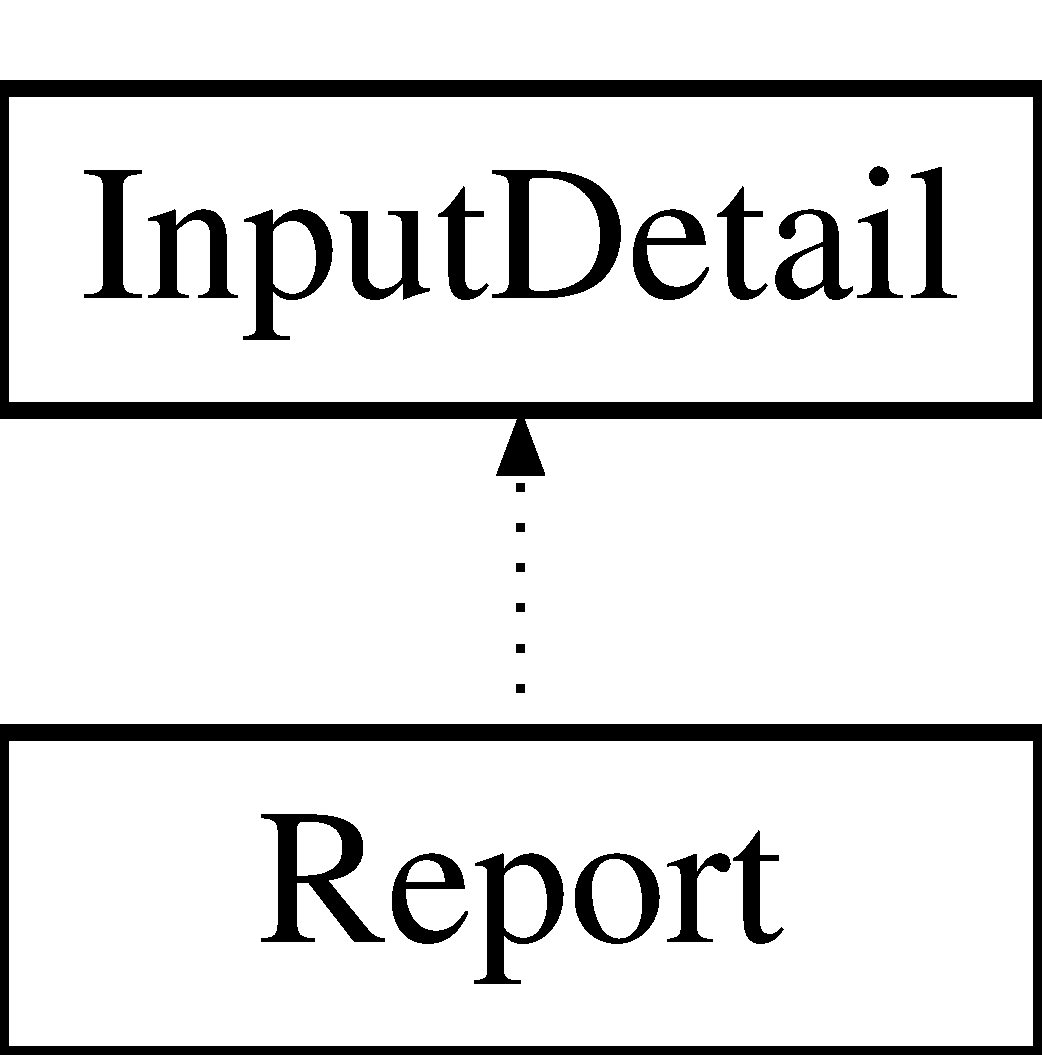
\includegraphics[height=3.000000cm]{classReport}
\end{center}
\end{figure}
\subsection*{Public Member Functions}
\begin{DoxyCompactItemize}
\item 
\hypertarget{classReport_a6b5a749dcbc19cb71503c5a6e2d465d3}{void {\bfseries Head} ()}\label{classReport_a6b5a749dcbc19cb71503c5a6e2d465d3}

\item 
\hypertarget{classReport_a97998b106d6fb7d6ccfea849892d21ee}{void {\bfseries Javascript} ()}\label{classReport_a97998b106d6fb7d6ccfea849892d21ee}

\item 
\hypertarget{classReport_a28dfc98e680194276c2bbb2fa4decf86}{void {\bfseries Body} ()}\label{classReport_a28dfc98e680194276c2bbb2fa4decf86}

\item 
\hypertarget{classReport_abfacfc97c910b8c2bc1a1102cc623d80}{void {\bfseries Body\-Content} ()}\label{classReport_abfacfc97c910b8c2bc1a1102cc623d80}

\item 
\hypertarget{classReport_a35895231f3a27c3247f9498cda2b42fe}{void {\bfseries Main} ()}\label{classReport_a35895231f3a27c3247f9498cda2b42fe}

\end{DoxyCompactItemize}
\subsection*{Additional Inherited Members}


The documentation for this class was generated from the following files\-:\begin{DoxyCompactItemize}
\item 
Baka\-Plan/report.\-h\item 
Baka\-Plan/report.\-cc\end{DoxyCompactItemize}

\hypertarget{classRollNoDetail}{\section{Roll\-No\-Detail Class Reference}
\label{classRollNoDetail}\index{Roll\-No\-Detail@{Roll\-No\-Detail}}
}


{\ttfamily \#include $<$rollnodetail.\-h$>$}

\subsection*{Public Member Functions}
\begin{DoxyCompactItemize}
\item 
\hyperlink{classRollNoDetail_a35022484630c725f33e0d9f70ee678d7}{Roll\-No\-Detail} ()
\begin{DoxyCompactList}\small\item\em Constructor. \end{DoxyCompactList}\item 
\hyperlink{classRollNoDetail_a941f09a9307b97c7d3655e68815954c3}{Read\-Class\-Details} ()
\begin{DoxyCompactList}\small\item\em Reading class details from previous page using cgicc. \end{DoxyCompactList}\item 
\hypertarget{classRollNoDetail_adeb8b51063f8e325c36472b8ab98557a}{{\bfseries Write\-Class\-Details} ()}\label{classRollNoDetail_adeb8b51063f8e325c36472b8ab98557a}

\end{DoxyCompactItemize}
\subsection*{Protected Attributes}
\begin{DoxyCompactItemize}
\item 
string \hyperlink{classRollNoDetail_af6210eb33a46b384c832560c9f1ebf07}{prefix} \mbox{[}M\-I\-N\-\_\-\-S\-I\-Z\-E\mbox{]}
\begin{DoxyCompactList}\small\item\em for storing values of class details \end{DoxyCompactList}\item 
\hypertarget{classRollNoDetail_ad093a47700148161f6bb299699ed8ff1}{string {\bfseries start\-Roll\-No} \mbox{[}M\-I\-N\-\_\-\-S\-I\-Z\-E\mbox{]}}\label{classRollNoDetail_ad093a47700148161f6bb299699ed8ff1}

\item 
\hypertarget{classRollNoDetail_a4eb0c44518937595bd377d40292422f9}{string {\bfseries end\-Roll\-No} \mbox{[}M\-I\-N\-\_\-\-S\-I\-Z\-E\mbox{]}}\label{classRollNoDetail_a4eb0c44518937595bd377d40292422f9}

\item 
\hypertarget{classRollNoDetail_aad7c0a0f7d5e854737a5fecfb4b745ca}{string {\bfseries not\-Included} \mbox{[}M\-I\-N\-\_\-\-S\-I\-Z\-E\mbox{]}}\label{classRollNoDetail_aad7c0a0f7d5e854737a5fecfb4b745ca}

\item 
\hypertarget{classRollNoDetail_ad904c7f4cf276df50d76651b5c4255c7}{int {\bfseries total\-Classes}}\label{classRollNoDetail_ad904c7f4cf276df50d76651b5c4255c7}

\end{DoxyCompactItemize}


\subsection{Detailed Description}
-\/-\/-\/-\/-\/-\/-\/-\/-\/-\/-\/-\/-\/-\/-\/-\/-\/-\/-\/-\/-\/-\/-\/-\/-\/-\/-\/-\/-\/-\/-\/-\/-\/-\/-\/-\/-\/-\/-\/-\/-\/-\/-\/-\/-\/-\/-\/-\/-\/-\/-\/-\/-\/-\/-\/-\/-\/-\/-\/-\/-\/-\/-\/-\/-\/-\/-\/ Include required header files ------------------------------------------------------------------ =================================================================== Class\-: \hyperlink{classRollNoDetail}{Roll\-No\-Detail} Description\-: \hyperlink{classRollNoDetail}{Roll\-No\-Detail} class for =================================================================== 

Definition at line 33 of file rollnodetail.\-h.



\subsection{Constructor \& Destructor Documentation}
\hypertarget{classRollNoDetail_a35022484630c725f33e0d9f70ee678d7}{\index{Roll\-No\-Detail@{Roll\-No\-Detail}!Roll\-No\-Detail@{Roll\-No\-Detail}}
\index{Roll\-No\-Detail@{Roll\-No\-Detail}!RollNoDetail@{Roll\-No\-Detail}}
\subsubsection[{Roll\-No\-Detail}]{\setlength{\rightskip}{0pt plus 5cm}Roll\-No\-Detail\-::\-Roll\-No\-Detail (
\begin{DoxyParamCaption}
{}
\end{DoxyParamCaption}
)}}\label{classRollNoDetail_a35022484630c725f33e0d9f70ee678d7}


Constructor. 

-\/-\/-\/-\/-\/-\/-\/-\/-\/-\/-\/-\/-\/-\/-\/-\/-\/-\/-\/-\/-\/-\/-\/-\/-\/-\/-\/-\/-\/-\/-\/-\/-\/-\/-\/-\/-\/-\/-\/-\/-\/-\/-\/-\/-\/-\/-\/-\/-\/-\/-\/-\/-\/-\/-\/-\/-\/-\/-\/-\/-\/-\/-\/-\/-\/-\/-\/ Include rollnodetails.\-h for \hyperlink{classRollNoDetail}{Roll\-No\-Detail} class declaration ------------------------------------------------------------------ -\/-\/-\/-\/-\/-\/-\/-\/-\/-\/-\/-\/-\/-\/-\/-\/-\/-\/-\/-\/-\/-\/-\/-\/-\/-\/-\/-\/-\/-\/-\/-\/-\/-\/-\/-\/-\/-\/-\/-\/-\/-\/-\/-\/-\/-\/-\/-\/-\/-\/-\/-\/-\/-\/-\/-\/-\/-\/-\/-\/-\/-\/-\/-\/-\/-\/-\/ Definition of functions \hyperlink{classRollNoDetail}{Roll\-No\-Detail} Class ------------------------------------------------------------------ -\/-\/-\/-\/-\/-\/-\/-\/-\/-\/-\/-\/-\/-\/-\/-\/-\/-\/-\/-\/-\/-\/-\/-\/-\/-\/-\/-\/-\/-\/-\/-\/-\/-\/-\/-\/-\/-\/-\/-\/-\/-\/-\/-\/-\/-\/-\/-\/-\/-\/-\/-\/-\/-\/-\/-\/-\/-\/-\/-\/-\/-\/-\/-\/-\/-\/-\/-\/ Class\-: \hyperlink{classRollNoDetail}{Roll\-No\-Detail} Method\-: \hyperlink{classRollNoDetail}{Roll\-No\-Detail} \-:\-: \hyperlink{classRollNoDetail_a35022484630c725f33e0d9f70ee678d7}{Roll\-No\-Detail()} Description\-: Constructor -\/-\/-\/-\/-\/-\/-\/-\/-\/-\/-\/-\/-\/-\/-\/-\/-\/-\/-\/-\/-\/-\/-\/-\/-\/-\/-\/-\/-\/-\/-\/-\/-\/-\/-\/-\/-\/-\/-\/-\/-\/-\/-\/-\/-\/-\/-\/-\/-\/-\/-\/-\/-\/-\/-\/-\/-\/-\/-\/-\/-\/-\/-\/-\/-\/-\/-\/-\/ 

Definition at line 37 of file rollnodetail.\-cc.



\subsection{Member Function Documentation}
\hypertarget{classRollNoDetail_a941f09a9307b97c7d3655e68815954c3}{\index{Roll\-No\-Detail@{Roll\-No\-Detail}!Read\-Class\-Details@{Read\-Class\-Details}}
\index{Read\-Class\-Details@{Read\-Class\-Details}!RollNoDetail@{Roll\-No\-Detail}}
\subsubsection[{Read\-Class\-Details}]{\setlength{\rightskip}{0pt plus 5cm}void Roll\-No\-Detail\-::\-Read\-Class\-Details (
\begin{DoxyParamCaption}
{}
\end{DoxyParamCaption}
)}}\label{classRollNoDetail_a941f09a9307b97c7d3655e68815954c3}


Reading class details from previous page using cgicc. 

-\/-\/-\/-\/-\/-\/-\/-\/-\/-\/-\/-\/-\/-\/-\/-\/-\/-\/-\/-\/-\/-\/-\/-\/-\/-\/-\/-\/-\/-\/-\/-\/-\/-\/-\/-\/-\/-\/-\/-\/-\/-\/-\/-\/-\/-\/-\/-\/-\/-\/-\/-\/-\/-\/-\/-\/-\/-\/-\/-\/-\/-\/-\/-\/-\/-\/-\/-\/ Class\-: \hyperlink{classRollNoDetail}{Roll\-No\-Detail} Method\-: \hyperlink{classRollNoDetail}{Roll\-No\-Detail} \-:\-: \hyperlink{classRollNoDetail_a941f09a9307b97c7d3655e68815954c3}{Read\-Class\-Details()} Description\-: For reading class details from previous page -\/-\/-\/-\/-\/-\/-\/-\/-\/-\/-\/-\/-\/-\/-\/-\/-\/-\/-\/-\/-\/-\/-\/-\/-\/-\/-\/-\/-\/-\/-\/-\/-\/-\/-\/-\/-\/-\/-\/-\/-\/-\/-\/-\/-\/-\/-\/-\/-\/-\/-\/-\/-\/-\/-\/-\/-\/-\/-\/-\/-\/-\/-\/-\/-\/-\/-\/-\/ 

Definition at line 50 of file rollnodetail.\-cc.



\subsection{Member Data Documentation}
\hypertarget{classRollNoDetail_af6210eb33a46b384c832560c9f1ebf07}{\index{Roll\-No\-Detail@{Roll\-No\-Detail}!prefix@{prefix}}
\index{prefix@{prefix}!RollNoDetail@{Roll\-No\-Detail}}
\subsubsection[{prefix}]{\setlength{\rightskip}{0pt plus 5cm}string Roll\-No\-Detail\-::prefix\mbox{[}M\-I\-N\-\_\-\-S\-I\-Z\-E\mbox{]}\hspace{0.3cm}{\ttfamily [protected]}}}\label{classRollNoDetail_af6210eb33a46b384c832560c9f1ebf07}


for storing values of class details 



Definition at line 37 of file rollnodetail.\-h.



The documentation for this class was generated from the following files\-:\begin{DoxyCompactItemize}
\item 
src/rollnodetail.\-h\item 
src/rollnodetail.\-cc\end{DoxyCompactItemize}

\hypertarget{classRoomDetail}{\section{\-Room\-Detail \-Class \-Reference}
\label{classRoomDetail}\index{\-Room\-Detail@{\-Room\-Detail}}
}


{\ttfamily \#include $<$room.\-h$>$}

\-Inheritance diagram for \-Room\-Detail\-:\begin{figure}[H]
\begin{center}
\leavevmode
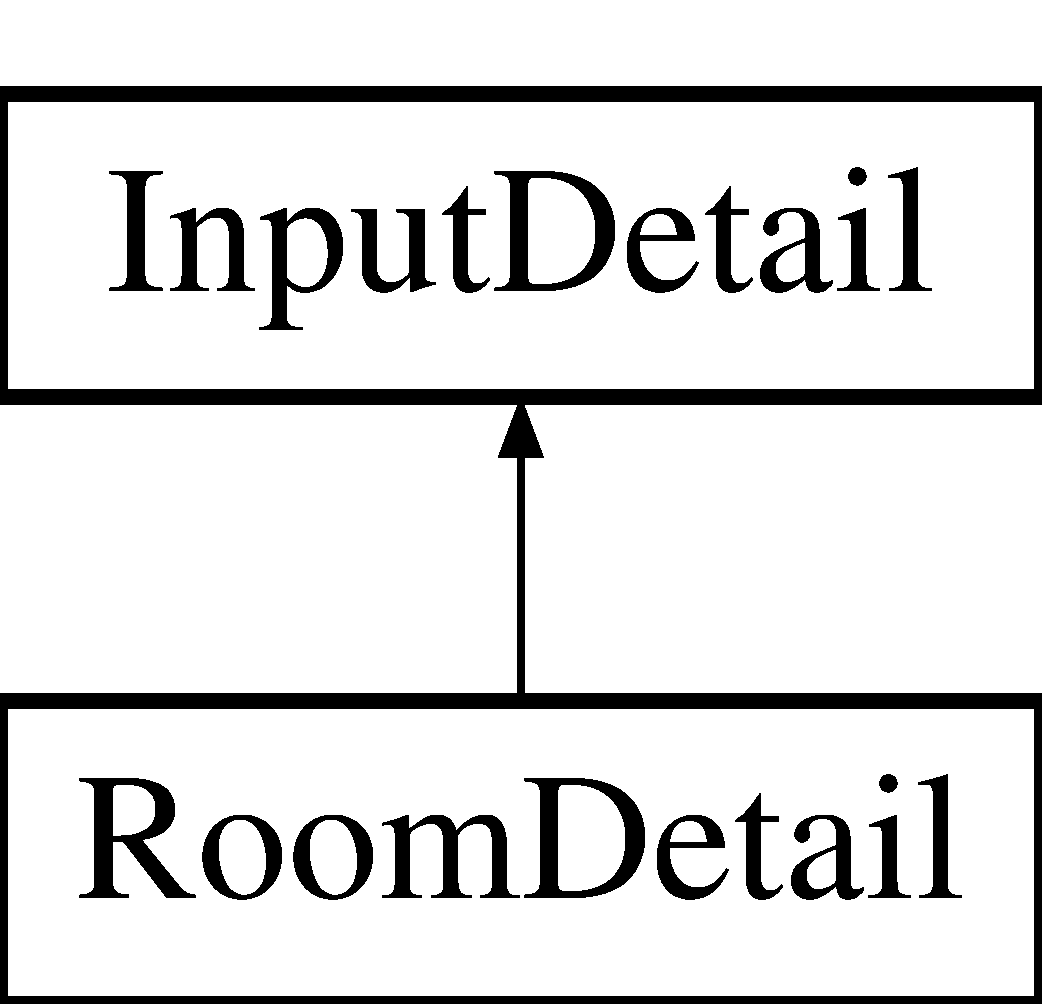
\includegraphics[height=2.000000cm]{classRoomDetail}
\end{center}
\end{figure}
\subsection*{\-Public \-Member \-Functions}
\begin{DoxyCompactItemize}
\item 
\hyperlink{classRoomDetail_acbbb21580bc1591daf23e614011acc06}{\-Room\-Detail} ()
\begin{DoxyCompactList}\small\item\em \-Constructor. \end{DoxyCompactList}\item 
void \hyperlink{classRoomDetail_a117bed37b0f95b364b7133fe13afa9b7}{\-Set\-Default\-Value} ()
\item 
void \hyperlink{classRoomDetail_ab8a07fd05ab314e85b374191e38e8556}{\-Read\-Date\-Sheet} ()
\begin{DoxyCompactList}\small\item\em \-Reading \-Date sheet \-I/\-P given by user. \end{DoxyCompactList}\item 
void \hyperlink{classRoomDetail_a90d4fc5bf3497068efecb5c9ec13e887}{\-Write\-Date\-Sheet} ()
\begin{DoxyCompactList}\small\item\em \-Writing \-Date \-Sheet into database. \end{DoxyCompactList}\item 
void \hyperlink{classRoomDetail_ab2c0a691ce4dea82d16f991c66021931}{\-Room\-Detail\-Page} (bool add\-Room)
\begin{DoxyCompactList}\small\item\em \-For \-Taking \-I/\-P from user of room details. \end{DoxyCompactList}\item 
void \hyperlink{classRoomDetail_ac4d4701717acda86a95c68ef5abbab28}{\-Add\-More\-Rooms} ()
\item 
\hyperlink{classRoomDetail_ae65b9b167e75a7dc994c4e2021937c68}{$\sim$\-Room\-Detail} ()
\begin{DoxyCompactList}\small\item\em \-Destructor to de-\/allocate objects. \end{DoxyCompactList}\end{DoxyCompactItemize}
\subsection*{\-Protected \-Attributes}
\begin{DoxyCompactItemize}
\item 
\hypertarget{classRoomDetail_a9bb16ea944d271f428cb36617c051ecd}{\hyperlink{classDateSheet}{\-Date\-Sheet} {\bfseries date\-Wise\-Roll\-No}}\label{classRoomDetail_a9bb16ea944d271f428cb36617c051ecd}

\end{DoxyCompactItemize}


\subsection{\-Detailed \-Description}
include inpudetail.\-h

\-Include \hyperlink{room_8h}{room.\-h} 

\-Definition at line 26 of file room.\-h.



\subsection{\-Constructor \& \-Destructor \-Documentation}
\hypertarget{classRoomDetail_acbbb21580bc1591daf23e614011acc06}{\index{\-Room\-Detail@{\-Room\-Detail}!\-Room\-Detail@{\-Room\-Detail}}
\index{\-Room\-Detail@{\-Room\-Detail}!RoomDetail@{\-Room\-Detail}}
\subsubsection[{\-Room\-Detail}]{\setlength{\rightskip}{0pt plus 5cm}{\bf \-Room\-Detail\-::\-Room\-Detail} (
\begin{DoxyParamCaption}
{}
\end{DoxyParamCaption}
)}}\label{classRoomDetail_acbbb21580bc1591daf23e614011acc06}


\-Constructor. 

\-Constructor 

\-Definition at line 27 of file room.\-cc.

\hypertarget{classRoomDetail_ae65b9b167e75a7dc994c4e2021937c68}{\index{\-Room\-Detail@{\-Room\-Detail}!$\sim$\-Room\-Detail@{$\sim$\-Room\-Detail}}
\index{$\sim$\-Room\-Detail@{$\sim$\-Room\-Detail}!RoomDetail@{\-Room\-Detail}}
\subsubsection[{$\sim$\-Room\-Detail}]{\setlength{\rightskip}{0pt plus 5cm}{\bf \-Room\-Detail\-::$\sim$\-Room\-Detail} (
\begin{DoxyParamCaption}
{}
\end{DoxyParamCaption}
)}}\label{classRoomDetail_ae65b9b167e75a7dc994c4e2021937c68}


\-Destructor to de-\/allocate objects. 

\-Desctructor 

\-Definition at line 491 of file room.\-cc.



\subsection{\-Member \-Function \-Documentation}
\hypertarget{classRoomDetail_ac4d4701717acda86a95c68ef5abbab28}{\index{\-Room\-Detail@{\-Room\-Detail}!\-Add\-More\-Rooms@{\-Add\-More\-Rooms}}
\index{\-Add\-More\-Rooms@{\-Add\-More\-Rooms}!RoomDetail@{\-Room\-Detail}}
\subsubsection[{\-Add\-More\-Rooms}]{\setlength{\rightskip}{0pt plus 5cm}void {\bf \-Room\-Detail\-::\-Add\-More\-Rooms} (
\begin{DoxyParamCaption}
{}
\end{DoxyParamCaption}
)}}\label{classRoomDetail_ac4d4701717acda86a95c68ef5abbab28}
\-Add \-More rooms if strategy in valid 

\-Definition at line 463 of file room.\-cc.

\hypertarget{classRoomDetail_ab8a07fd05ab314e85b374191e38e8556}{\index{\-Room\-Detail@{\-Room\-Detail}!\-Read\-Date\-Sheet@{\-Read\-Date\-Sheet}}
\index{\-Read\-Date\-Sheet@{\-Read\-Date\-Sheet}!RoomDetail@{\-Room\-Detail}}
\subsubsection[{\-Read\-Date\-Sheet}]{\setlength{\rightskip}{0pt plus 5cm}void {\bf \-Room\-Detail\-::\-Read\-Date\-Sheet} (
\begin{DoxyParamCaption}
{}
\end{DoxyParamCaption}
)}}\label{classRoomDetail_ab8a07fd05ab314e85b374191e38e8556}


\-Reading \-Date sheet \-I/\-P given by user. 

\-Reading \-Datesheet 

\-Definition at line 140 of file room.\-cc.

\hypertarget{classRoomDetail_ab2c0a691ce4dea82d16f991c66021931}{\index{\-Room\-Detail@{\-Room\-Detail}!\-Room\-Detail\-Page@{\-Room\-Detail\-Page}}
\index{\-Room\-Detail\-Page@{\-Room\-Detail\-Page}!RoomDetail@{\-Room\-Detail}}
\subsubsection[{\-Room\-Detail\-Page}]{\setlength{\rightskip}{0pt plus 5cm}void {\bf \-Room\-Detail\-::\-Room\-Detail\-Page} (
\begin{DoxyParamCaption}
\item[{bool}]{add\-Room}
\end{DoxyParamCaption}
)}}\label{classRoomDetail_ab2c0a691ce4dea82d16f991c66021931}


\-For \-Taking \-I/\-P from user of room details. 

\-Room \-D\-Etail page for taking \-I/\-P from user 

\-Definition at line 239 of file room.\-cc.

\hypertarget{classRoomDetail_a117bed37b0f95b364b7133fe13afa9b7}{\index{\-Room\-Detail@{\-Room\-Detail}!\-Set\-Default\-Value@{\-Set\-Default\-Value}}
\index{\-Set\-Default\-Value@{\-Set\-Default\-Value}!RoomDetail@{\-Room\-Detail}}
\subsubsection[{\-Set\-Default\-Value}]{\setlength{\rightskip}{0pt plus 5cm}void {\bf \-Room\-Detail\-::\-Set\-Default\-Value} (
\begin{DoxyParamCaption}
{}
\end{DoxyParamCaption}
)}}\label{classRoomDetail_a117bed37b0f95b364b7133fe13afa9b7}
\-Set \-Default \-Value 

\-Definition at line 47 of file room.\-cc.

\hypertarget{classRoomDetail_a90d4fc5bf3497068efecb5c9ec13e887}{\index{\-Room\-Detail@{\-Room\-Detail}!\-Write\-Date\-Sheet@{\-Write\-Date\-Sheet}}
\index{\-Write\-Date\-Sheet@{\-Write\-Date\-Sheet}!RoomDetail@{\-Room\-Detail}}
\subsubsection[{\-Write\-Date\-Sheet}]{\setlength{\rightskip}{0pt plus 5cm}void {\bf \-Room\-Detail\-::\-Write\-Date\-Sheet} (
\begin{DoxyParamCaption}
{}
\end{DoxyParamCaption}
)}}\label{classRoomDetail_a90d4fc5bf3497068efecb5c9ec13e887}


\-Writing \-Date \-Sheet into database. 

\-Writing \hyperlink{classDateSheet}{\-Date\-Sheet} 

\-Definition at line 185 of file room.\-cc.



\-The documentation for this class was generated from the following files\-:\begin{DoxyCompactItemize}
\item 
frontend/src/header/\hyperlink{room_8h}{room.\-h}\item 
frontend/src/\hyperlink{room_8cc}{room.\-cc}\end{DoxyCompactItemize}

\hypertarget{classSeatPlan}{\section{Seat\-Plan Class Reference}
\label{classSeatPlan}\index{Seat\-Plan@{Seat\-Plan}}
}


\hyperlink{classSeatPlan}{Seat\-Plan} C\-Lass for generating seating plan.  




{\ttfamily \#include $<$report.\-h$>$}

Inheritance diagram for Seat\-Plan\-:\begin{figure}[H]
\begin{center}
\leavevmode
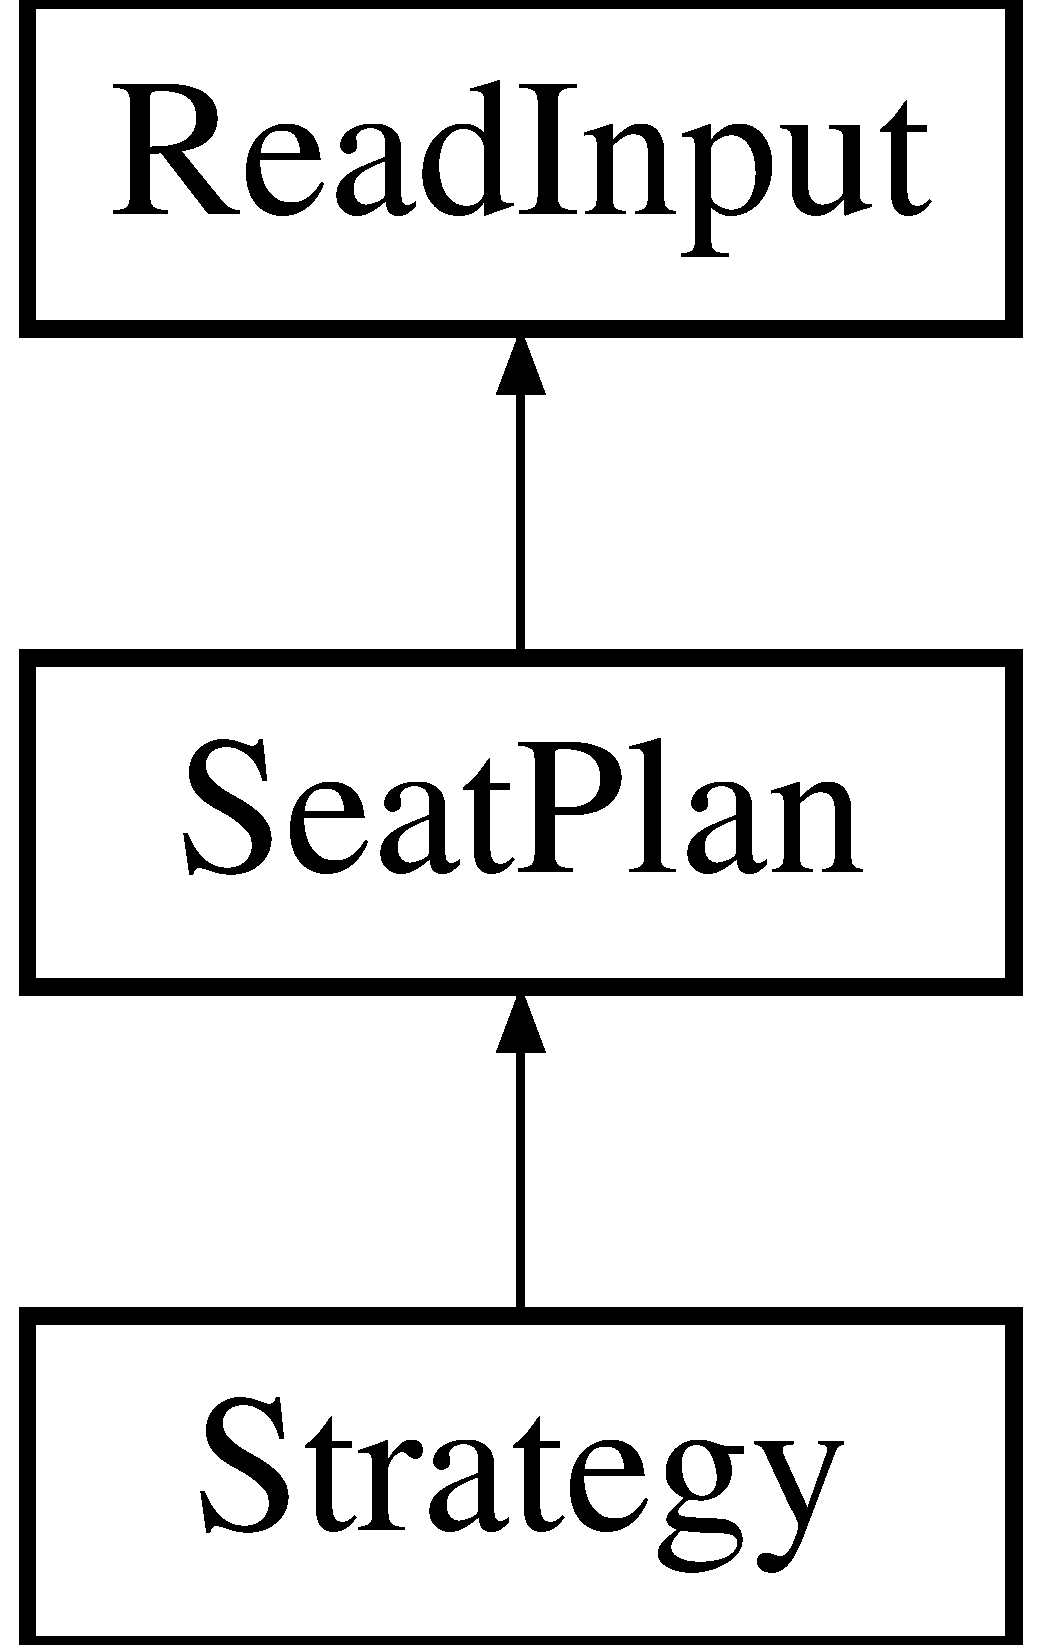
\includegraphics[height=3.000000cm]{classSeatPlan}
\end{center}
\end{figure}
\subsection*{Public Member Functions}
\begin{DoxyCompactItemize}
\item 
\hyperlink{classSeatPlan_a974a336df39c9fefc2b239a382a4749c}{Room\-Report} ()
\item 
void \hyperlink{classSeatPlan_ae93cefd4fd0401c5d54b8e97b23541ae}{Read\-Exam\-Detail} (string \hyperlink{classReadInput_a3ad470a25b3e0a29466bf4ff1f7d8e81}{project\-I\-D})
\item 
void \hyperlink{classSeatPlan_a618d148beefee9d4db3d038328c9b2c8}{Read\-Seat\-Plan} (string \hyperlink{classReadInput_a3ad470a25b3e0a29466bf4ff1f7d8e81}{project\-I\-D})
\item 
void \hyperlink{classSeatPlan_af572f79142f4dad362f54892c6747214}{Write\-H\-T\-M\-L\-File} (string \hyperlink{classReadInput_a3ad470a25b3e0a29466bf4ff1f7d8e81}{project\-I\-D})
\item 
\hyperlink{classSeatPlan_a446949506a25bcda5eb972c8a4b1384d}{$\sim$\-Room\-Report} ()
\item 
\hyperlink{classSeatPlan_ab1906186f96847704ed71f1a6c738327}{Seat\-Plan} ()
\begin{DoxyCompactList}\small\item\em Constructor. \end{DoxyCompactList}\item 
\hypertarget{classSeatPlan_afa418b9edadff831c73ea6005666becf}{void {\bfseries Set\-Roll\-No} (int strategy, int i)}\label{classSeatPlan_afa418b9edadff831c73ea6005666becf}

\item 
\hypertarget{classSeatPlan_a3dfc44c97eab7f3d33f2023ae0faaa13}{string {\bfseries Roll\-No} (int s)}\label{classSeatPlan_a3dfc44c97eab7f3d33f2023ae0faaa13}

\item 
\hypertarget{classSeatPlan_a1df3b03c983936c07225ed1a79959f1b}{void {\bfseries Seating\-Plan} (int strategy, int i)}\label{classSeatPlan_a1df3b03c983936c07225ed1a79959f1b}

\item 
\hypertarget{classSeatPlan_ade684c0f63b648d4d62df8e7ed800682}{void {\bfseries Create\-File} (string \hyperlink{classReadInput_a3ad470a25b3e0a29466bf4ff1f7d8e81}{project\-I\-D})}\label{classSeatPlan_ade684c0f63b648d4d62df8e7ed800682}

\item 
\hypertarget{classSeatPlan_a3f29cad9d9be46f7bc3055de2ab887fc}{void {\bfseries Write\-Seat\-Plan} (string \hyperlink{classReadInput_a3ad470a25b3e0a29466bf4ff1f7d8e81}{project\-I\-D}, int i)}\label{classSeatPlan_a3f29cad9d9be46f7bc3055de2ab887fc}

\item 
void \hyperlink{classSeatPlan_a67c10e2277f1f2823581cddf4df373c5}{Write\-H\-T\-M\-L\-File} (string \hyperlink{classReadInput_a3ad470a25b3e0a29466bf4ff1f7d8e81}{project\-I\-D}, int i)
\begin{DoxyCompactList}\small\item\em Creating H\-T\-M\-L file. \end{DoxyCompactList}\item 
\hypertarget{classSeatPlan_abce0c5b5545f1bb1ebcf2e578b6ab282}{void {\bfseries Write\-P\-D\-F\-File} (string \hyperlink{classReadInput_a3ad470a25b3e0a29466bf4ff1f7d8e81}{project\-I\-D}, int i)}\label{classSeatPlan_abce0c5b5545f1bb1ebcf2e578b6ab282}

\item 
\hypertarget{classSeatPlan_a3257eb25ac9c82d2757d2a7144614762}{void {\bfseries Add\-Roll\-No\-Info} (string \hyperlink{classReadInput_a3ad470a25b3e0a29466bf4ff1f7d8e81}{project\-I\-D}, int i)}\label{classSeatPlan_a3257eb25ac9c82d2757d2a7144614762}

\item 
\hyperlink{classSeatPlan_a373a1d60b6617a2e424f7d2f8866ec2e}{$\sim$\-Seat\-Plan} ()
\begin{DoxyCompactList}\small\item\em D\-Estructor. \end{DoxyCompactList}\end{DoxyCompactItemize}
\subsection*{Protected Attributes}
\begin{DoxyCompactItemize}
\item 
\hypertarget{classSeatPlan_a6915f74be45af73cda8c9a51b6cb99c9}{int {\bfseries total\-Seats}}\label{classSeatPlan_a6915f74be45af73cda8c9a51b6cb99c9}

\item 
\hypertarget{classSeatPlan_a3568dfc375740fd6b4075d7dc419a2e5}{int {\bfseries total\-Students}}\label{classSeatPlan_a3568dfc375740fd6b4075d7dc419a2e5}

\item 
\hypertarget{classSeatPlan_a18b1d6497343d6a9e751159dcdd8a179}{int {\bfseries total\-Group\-Seats}}\label{classSeatPlan_a18b1d6497343d6a9e751159dcdd8a179}

\item 
\hypertarget{classSeatPlan_acf6fa47342ec7f5675064c5601800f5c}{int {\bfseries day}}\label{classSeatPlan_acf6fa47342ec7f5675064c5601800f5c}

\item 
\hypertarget{classSeatPlan_a19a423aff33092a242f5dff5694efa37}{I\-N\-T\-\_\-\-V\-E\-C {\bfseries i\-Temp}}\label{classSeatPlan_a19a423aff33092a242f5dff5694efa37}

\item 
\hypertarget{classSeatPlan_af3fbce455c6744dee3fedb97442cd2c3}{I\-N\-T\-\_\-\-V\-E\-C {\bfseries index\-Value}}\label{classSeatPlan_af3fbce455c6744dee3fedb97442cd2c3}

\item 
\hypertarget{classSeatPlan_a6cb00329d2f0760f679d7e00958da879}{I\-N\-T\-\_\-\-V\-E\-C {\bfseries group\-Student\-Size}}\label{classSeatPlan_a6cb00329d2f0760f679d7e00958da879}

\item 
\hypertarget{classSeatPlan_a73de1d93e86c3a23406e0903c546ea2c}{I\-N\-T\-\_\-\-V\-E\-C {\bfseries seat\-Size}}\label{classSeatPlan_a73de1d93e86c3a23406e0903c546ea2c}

\item 
\hypertarget{classSeatPlan_a45d2c9c1d580d442bc15dcb50265d627}{I\-N\-T\-\_\-\-V\-E\-C {\bfseries size}}\label{classSeatPlan_a45d2c9c1d580d442bc15dcb50265d627}

\item 
\hypertarget{classSeatPlan_a52bafc6123bd54a8f95253c4693b2975}{I\-N\-T\-\_\-3\-D\-V\-E\-C {\bfseries room\-Size}}\label{classSeatPlan_a52bafc6123bd54a8f95253c4693b2975}

\item 
\hypertarget{classSeatPlan_ace374a7f84b7f9fb43fc56979a3793fb}{S\-T\-R\-I\-N\-G\-\_\-\-V\-E\-C {\bfseries sub\-Sub\-Code}}\label{classSeatPlan_ace374a7f84b7f9fb43fc56979a3793fb}

\item 
\hypertarget{classSeatPlan_adf8ed7579be4a43e20cbf4b40bb7b25e}{S\-T\-R\-I\-N\-G\-\_\-2\-D\-V\-E\-C {\bfseries seat\-Roll\-No}}\label{classSeatPlan_adf8ed7579be4a43e20cbf4b40bb7b25e}

\item 
\hypertarget{classSeatPlan_a38f161cde37bcfae5877a17f785cbb21}{S\-T\-R\-I\-N\-G\-\_\-2\-D\-V\-E\-C {\bfseries sub\-Roll\-No}}\label{classSeatPlan_a38f161cde37bcfae5877a17f785cbb21}

\item 
\hypertarget{classSeatPlan_a99f24fdf486af2b45bf142558011573d}{S\-T\-R\-I\-N\-G\-\_\-4\-D\-V\-E\-C {\bfseries seat}}\label{classSeatPlan_a99f24fdf486af2b45bf142558011573d}

\item 
\hypertarget{classSeatPlan_ac623e253b6005a0907c2dab61705f2ab}{int {\bfseries text\-Width}}\label{classSeatPlan_ac623e253b6005a0907c2dab61705f2ab}

\item 
\hypertarget{classSeatPlan_a2e67c39e7c6fff250ce3dc727f0680fd}{int {\bfseries text\-Width1}}\label{classSeatPlan_a2e67c39e7c6fff250ce3dc727f0680fd}

\item 
\hypertarget{classSeatPlan_aff452e60a99eb2582210d3ea7f454a32}{int {\bfseries rect\-Width}}\label{classSeatPlan_aff452e60a99eb2582210d3ea7f454a32}

\item 
\hypertarget{classSeatPlan_a878a765b96afb02615e7eb29bac8678d}{int {\bfseries x}}\label{classSeatPlan_a878a765b96afb02615e7eb29bac8678d}

\item 
\hypertarget{classSeatPlan_ab3a440c8ee63a36610340b1352d69f34}{int {\bfseries y}}\label{classSeatPlan_ab3a440c8ee63a36610340b1352d69f34}

\item 
\hypertarget{classSeatPlan_af13573b0c9227b8bba267fc9f3476f43}{int {\bfseries width}}\label{classSeatPlan_af13573b0c9227b8bba267fc9f3476f43}

\item 
\hypertarget{classSeatPlan_ad7a71523cc34692963985241fe942359}{int {\bfseries height}}\label{classSeatPlan_ad7a71523cc34692963985241fe942359}

\item 
\hypertarget{classSeatPlan_a55052a9b7a637609f439a003b0957552}{int {\bfseries centre}}\label{classSeatPlan_a55052a9b7a637609f439a003b0957552}

\item 
\hypertarget{classSeatPlan_ab01207ceddc85e4535874e2db71e36e3}{int {\bfseries room}}\label{classSeatPlan_ab01207ceddc85e4535874e2db71e36e3}

\item 
\hypertarget{classSeatPlan_a0b1f1e5086e938c3f484bbec62ff0dff}{int {\bfseries room1}}\label{classSeatPlan_a0b1f1e5086e938c3f484bbec62ff0dff}

\item 
\hypertarget{classSeatPlan_afcff743dbcb0e5c364cac4570730ad25}{int {\bfseries row}}\label{classSeatPlan_afcff743dbcb0e5c364cac4570730ad25}

\item 
\hypertarget{classSeatPlan_a959c1e5ee849ea93b5f46a98d4f45060}{int {\bfseries col}}\label{classSeatPlan_a959c1e5ee849ea93b5f46a98d4f45060}

\item 
\hypertarget{classSeatPlan_a31abf30876cae554e4a11f3b4892a93c}{int {\bfseries s}}\label{classSeatPlan_a31abf30876cae554e4a11f3b4892a93c}

\item 
\hypertarget{classSeatPlan_a03348c2da937f350737d7039dbd80cc8}{int {\bfseries start}}\label{classSeatPlan_a03348c2da937f350737d7039dbd80cc8}

\item 
\hypertarget{classSeatPlan_ade0c58a66a04c9f90803dee62954e15f}{int {\bfseries end}}\label{classSeatPlan_ade0c58a66a04c9f90803dee62954e15f}

\item 
\hypertarget{classSeatPlan_a2c85aa97b3681f2ba5e27af197836b26}{int {\bfseries index}}\label{classSeatPlan_a2c85aa97b3681f2ba5e27af197836b26}

\end{DoxyCompactItemize}


\subsection{Detailed Description}
\hyperlink{classSeatPlan}{Seat\-Plan} C\-Lass for generating seating plan. 

Include local header file

include \hyperlink{readinput_8h}{readinput.\-h}

include \hyperlink{seatplan_8h}{seatplan.\-h} file 

Definition at line 25 of file report.\-h.



\subsection{Constructor \& Destructor Documentation}
\hypertarget{classSeatPlan_a446949506a25bcda5eb972c8a4b1384d}{\index{Seat\-Plan@{Seat\-Plan}!$\sim$\-Room\-Report@{$\sim$\-Room\-Report}}
\index{$\sim$\-Room\-Report@{$\sim$\-Room\-Report}!SeatPlan@{Seat\-Plan}}
\subsubsection[{$\sim$\-Room\-Report}]{\setlength{\rightskip}{0pt plus 5cm}Seat\-Plan\-::$\sim$\-Room\-Report (
\begin{DoxyParamCaption}
{}
\end{DoxyParamCaption}
)}}\label{classSeatPlan_a446949506a25bcda5eb972c8a4b1384d}
Destructor \hypertarget{classSeatPlan_ab1906186f96847704ed71f1a6c738327}{\index{Seat\-Plan@{Seat\-Plan}!Seat\-Plan@{Seat\-Plan}}
\index{Seat\-Plan@{Seat\-Plan}!SeatPlan@{Seat\-Plan}}
\subsubsection[{Seat\-Plan}]{\setlength{\rightskip}{0pt plus 5cm}Seat\-Plan\-::\-Seat\-Plan (
\begin{DoxyParamCaption}
{}
\end{DoxyParamCaption}
)}}\label{classSeatPlan_ab1906186f96847704ed71f1a6c738327}


Constructor. 

Constructor 

Definition at line 28 of file seatplan.\-cc.

\hypertarget{classSeatPlan_a373a1d60b6617a2e424f7d2f8866ec2e}{\index{Seat\-Plan@{Seat\-Plan}!$\sim$\-Seat\-Plan@{$\sim$\-Seat\-Plan}}
\index{$\sim$\-Seat\-Plan@{$\sim$\-Seat\-Plan}!SeatPlan@{Seat\-Plan}}
\subsubsection[{$\sim$\-Seat\-Plan}]{\setlength{\rightskip}{0pt plus 5cm}Seat\-Plan\-::$\sim$\-Seat\-Plan (
\begin{DoxyParamCaption}
{}
\end{DoxyParamCaption}
)}}\label{classSeatPlan_a373a1d60b6617a2e424f7d2f8866ec2e}


D\-Estructor. 

Destructor 

Definition at line 593 of file seatplan.\-cc.



\subsection{Member Function Documentation}
\hypertarget{classSeatPlan_ae93cefd4fd0401c5d54b8e97b23541ae}{\index{Seat\-Plan@{Seat\-Plan}!Read\-Exam\-Detail@{Read\-Exam\-Detail}}
\index{Read\-Exam\-Detail@{Read\-Exam\-Detail}!SeatPlan@{Seat\-Plan}}
\subsubsection[{Read\-Exam\-Detail}]{\setlength{\rightskip}{0pt plus 5cm}void Seat\-Plan\-::\-Read\-Exam\-Detail (
\begin{DoxyParamCaption}
\item[{string}]{project\-I\-D}
\end{DoxyParamCaption}
)}}\label{classSeatPlan_ae93cefd4fd0401c5d54b8e97b23541ae}
Read Exam Detail \hypertarget{classSeatPlan_a618d148beefee9d4db3d038328c9b2c8}{\index{Seat\-Plan@{Seat\-Plan}!Read\-Seat\-Plan@{Read\-Seat\-Plan}}
\index{Read\-Seat\-Plan@{Read\-Seat\-Plan}!SeatPlan@{Seat\-Plan}}
\subsubsection[{Read\-Seat\-Plan}]{\setlength{\rightskip}{0pt plus 5cm}void Seat\-Plan\-::\-Read\-Seat\-Plan (
\begin{DoxyParamCaption}
\item[{string}]{project\-I\-D}
\end{DoxyParamCaption}
)}}\label{classSeatPlan_a618d148beefee9d4db3d038328c9b2c8}
Read Seat Plan \hypertarget{classSeatPlan_a974a336df39c9fefc2b239a382a4749c}{\index{Seat\-Plan@{Seat\-Plan}!Room\-Report@{Room\-Report}}
\index{Room\-Report@{Room\-Report}!SeatPlan@{Seat\-Plan}}
\subsubsection[{Room\-Report}]{\setlength{\rightskip}{0pt plus 5cm}Seat\-Plan\-::\-Room\-Report (
\begin{DoxyParamCaption}
{}
\end{DoxyParamCaption}
)}}\label{classSeatPlan_a974a336df39c9fefc2b239a382a4749c}
Constructor \hypertarget{classSeatPlan_af572f79142f4dad362f54892c6747214}{\index{Seat\-Plan@{Seat\-Plan}!Write\-H\-T\-M\-L\-File@{Write\-H\-T\-M\-L\-File}}
\index{Write\-H\-T\-M\-L\-File@{Write\-H\-T\-M\-L\-File}!SeatPlan@{Seat\-Plan}}
\subsubsection[{Write\-H\-T\-M\-L\-File}]{\setlength{\rightskip}{0pt plus 5cm}void Seat\-Plan\-::\-Write\-H\-T\-M\-L\-File (
\begin{DoxyParamCaption}
\item[{string}]{project\-I\-D}
\end{DoxyParamCaption}
)}}\label{classSeatPlan_af572f79142f4dad362f54892c6747214}
Write\-H\-T\-M\-L\-File \hypertarget{classSeatPlan_a67c10e2277f1f2823581cddf4df373c5}{\index{Seat\-Plan@{Seat\-Plan}!Write\-H\-T\-M\-L\-File@{Write\-H\-T\-M\-L\-File}}
\index{Write\-H\-T\-M\-L\-File@{Write\-H\-T\-M\-L\-File}!SeatPlan@{Seat\-Plan}}
\subsubsection[{Write\-H\-T\-M\-L\-File}]{\setlength{\rightskip}{0pt plus 5cm}void Seat\-Plan\-::\-Write\-H\-T\-M\-L\-File (
\begin{DoxyParamCaption}
\item[{string}]{project\-I\-D, }
\item[{int}]{i}
\end{DoxyParamCaption}
)}}\label{classSeatPlan_a67c10e2277f1f2823581cddf4df373c5}


Creating H\-T\-M\-L file. 


\begin{DoxyParams}{Parameters}
{\em project\-I\-D} & Project Id of seating plan project \\
\hline
{\em i} & For creating file accord to datesheet \\
\hline
\end{DoxyParams}


Definition at line 311 of file seatplan.\-cc.



The documentation for this class was generated from the following files\-:\begin{DoxyCompactItemize}
\item 
src/cpp/backend/header/\hyperlink{report_8h}{report.\-h}\item 
src/cpp/backend/header/\hyperlink{seatplan_8h}{seatplan.\-h}\item 
src/cpp/backend/\hyperlink{seatplan_8cc}{seatplan.\-cc}\end{DoxyCompactItemize}

\hypertarget{classSendMail}{\section{Send\-Mail Class Reference}
\label{classSendMail}\index{Send\-Mail@{Send\-Mail}}
}


Class for sending mail to user for registeration.  




{\ttfamily \#include $<$sendmail.\-h$>$}

\subsection*{Public Member Functions}
\begin{DoxyCompactItemize}
\item 
\hyperlink{classSendMail_ae0d11ddeda1ae7ae1cc3b8f11678ed92}{Send\-Mail} ()
\begin{DoxyCompactList}\small\item\em Constructor. \end{DoxyCompactList}\item 
void \hyperlink{classSendMail_a25ba5afabc97cf3dab525f2eb1e67e0e}{Set\-Mail\-Data} ()
\begin{DoxyCompactList}\small\item\em Settinf variable that are used to send mail. \end{DoxyCompactList}\item 
void \hyperlink{classSendMail_a89c5a5bace5c21014b8184db5707b986}{Set\-H\-T\-M\-L\-Message} (string reg\-Key, string mail)
\begin{DoxyCompactList}\small\item\em Setting body of mail(message ie send to user) \end{DoxyCompactList}\item 
void \hyperlink{classSendMail_a4c9983852dbcd1eb07170582761ed559}{Registration\-Mail} (string set\-Recipient, string reg\-Key)
\begin{DoxyCompactList}\small\item\em Sending registration mail to user. \end{DoxyCompactList}\item 
\hypertarget{classSendMail_a56180b5a27efd4d43514f91008b280ef}{void {\bfseries Reset\-Password\-Mail} (string set\-Recipient, string reg\-Key)}\label{classSendMail_a56180b5a27efd4d43514f91008b280ef}

\item 
\hyperlink{classSendMail_acc86b2a9995472436dbd77b3c6bb91f3}{$\sim$\-Send\-Mail} ()
\begin{DoxyCompactList}\small\item\em Destructor. \end{DoxyCompactList}\end{DoxyCompactItemize}
\subsection*{Protected Attributes}
\begin{DoxyCompactItemize}
\item 
\hypertarget{classSendMail_ae6776dfd1b92b97837f25259f7b57d2f}{string {\bfseries set\-Sender}}\label{classSendMail_ae6776dfd1b92b97837f25259f7b57d2f}

\item 
\hypertarget{classSendMail_a22e32135e60ad02a6beff91638907cc6}{string {\bfseries set\-Subject}}\label{classSendMail_a22e32135e60ad02a6beff91638907cc6}

\item 
\hypertarget{classSendMail_ac4e386f1e7775484429f7b01ef1623a3}{string {\bfseries set\-Message}}\label{classSendMail_ac4e386f1e7775484429f7b01ef1623a3}

\item 
\hypertarget{classSendMail_a5337895c22cda4db5ebd05e43925e391}{string {\bfseries set\-Server}}\label{classSendMail_a5337895c22cda4db5ebd05e43925e391}

\item 
\hypertarget{classSendMail_a962ca34d61eab5c0f8c47e760cce4a53}{string {\bfseries html\-Message}}\label{classSendMail_a962ca34d61eab5c0f8c47e760cce4a53}

\item 
\hypertarget{classSendMail_a6b02c708619c2fb35216b2ee3061f33b}{string {\bfseries url}}\label{classSendMail_a6b02c708619c2fb35216b2ee3061f33b}

\end{DoxyCompactItemize}


\subsection{Detailed Description}
Class for sending mail to user for registeration. 

Include \hyperlink{sendmail_8h}{sendmail.\-h} 

Definition at line 39 of file sendmail.\-h.



\subsection{Constructor \& Destructor Documentation}
\hypertarget{classSendMail_ae0d11ddeda1ae7ae1cc3b8f11678ed92}{\index{Send\-Mail@{Send\-Mail}!Send\-Mail@{Send\-Mail}}
\index{Send\-Mail@{Send\-Mail}!SendMail@{Send\-Mail}}
\subsubsection[{Send\-Mail}]{\setlength{\rightskip}{0pt plus 5cm}Send\-Mail\-::\-Send\-Mail (
\begin{DoxyParamCaption}
{}
\end{DoxyParamCaption}
)}}\label{classSendMail_ae0d11ddeda1ae7ae1cc3b8f11678ed92}


Constructor. 

Constructor 

Definition at line 28 of file sendmail.\-cc.

\hypertarget{classSendMail_acc86b2a9995472436dbd77b3c6bb91f3}{\index{Send\-Mail@{Send\-Mail}!$\sim$\-Send\-Mail@{$\sim$\-Send\-Mail}}
\index{$\sim$\-Send\-Mail@{$\sim$\-Send\-Mail}!SendMail@{Send\-Mail}}
\subsubsection[{$\sim$\-Send\-Mail}]{\setlength{\rightskip}{0pt plus 5cm}Send\-Mail\-::$\sim$\-Send\-Mail (
\begin{DoxyParamCaption}
{}
\end{DoxyParamCaption}
)}}\label{classSendMail_acc86b2a9995472436dbd77b3c6bb91f3}


Destructor. 

Desrtuctor 

Definition at line 133 of file sendmail.\-cc.



\subsection{Member Function Documentation}
\hypertarget{classSendMail_a4c9983852dbcd1eb07170582761ed559}{\index{Send\-Mail@{Send\-Mail}!Registration\-Mail@{Registration\-Mail}}
\index{Registration\-Mail@{Registration\-Mail}!SendMail@{Send\-Mail}}
\subsubsection[{Registration\-Mail}]{\setlength{\rightskip}{0pt plus 5cm}void Send\-Mail\-::\-Registration\-Mail (
\begin{DoxyParamCaption}
\item[{string}]{set\-Recipient, }
\item[{string}]{reg\-Key}
\end{DoxyParamCaption}
)}}\label{classSendMail_a4c9983852dbcd1eb07170582761ed559}


Sending registration mail to user. 

Function for sending mail to new user(registeration link)


\begin{DoxyParams}{Parameters}
{\em } & \\
\hline
\end{DoxyParams}


Definition at line 87 of file sendmail.\-cc.

\hypertarget{classSendMail_a89c5a5bace5c21014b8184db5707b986}{\index{Send\-Mail@{Send\-Mail}!Set\-H\-T\-M\-L\-Message@{Set\-H\-T\-M\-L\-Message}}
\index{Set\-H\-T\-M\-L\-Message@{Set\-H\-T\-M\-L\-Message}!SendMail@{Send\-Mail}}
\subsubsection[{Set\-H\-T\-M\-L\-Message}]{\setlength{\rightskip}{0pt plus 5cm}void Send\-Mail\-::\-Set\-H\-T\-M\-L\-Message (
\begin{DoxyParamCaption}
\item[{string}]{reg\-Key, }
\item[{string}]{mail}
\end{DoxyParamCaption}
)}}\label{classSendMail_a89c5a5bace5c21014b8184db5707b986}


Setting body of mail(message ie send to user) 

Setting message of mail


\begin{DoxyParams}{Parameters}
{\em reg\-Key} & Registration Key \\
\hline
\end{DoxyParams}


Definition at line 53 of file sendmail.\-cc.

\hypertarget{classSendMail_a25ba5afabc97cf3dab525f2eb1e67e0e}{\index{Send\-Mail@{Send\-Mail}!Set\-Mail\-Data@{Set\-Mail\-Data}}
\index{Set\-Mail\-Data@{Set\-Mail\-Data}!SendMail@{Send\-Mail}}
\subsubsection[{Set\-Mail\-Data}]{\setlength{\rightskip}{0pt plus 5cm}void Send\-Mail\-::\-Set\-Mail\-Data (
\begin{DoxyParamCaption}
{}
\end{DoxyParamCaption}
)}}\label{classSendMail_a25ba5afabc97cf3dab525f2eb1e67e0e}


Settinf variable that are used to send mail. 

Setting variables 

Definition at line 39 of file sendmail.\-cc.



The documentation for this class was generated from the following files\-:\begin{DoxyCompactItemize}
\item 
frontend/src/header/\hyperlink{sendmail_8h}{sendmail.\-h}\item 
frontend/src/\hyperlink{sendmail_8cc}{sendmail.\-cc}\end{DoxyCompactItemize}

\hypertarget{classStrategy}{\section{Strategy Class Reference}
\label{classStrategy}\index{Strategy@{Strategy}}
}


\subsection{Detailed Description}
include strategy.\-h 

The documentation for this class was generated from the following file\-:\begin{DoxyCompactItemize}
\item 
frontend/src/backend/strategy.\-cc\end{DoxyCompactItemize}

\hypertarget{classValidStrategy}{\section{Valid\-Strategy Class Reference}
\label{classValidStrategy}\index{Valid\-Strategy@{Valid\-Strategy}}
}


{\ttfamily \#include $<$validstrategy.\-h$>$}

Inheritance diagram for Valid\-Strategy\-:\begin{figure}[H]
\begin{center}
\leavevmode
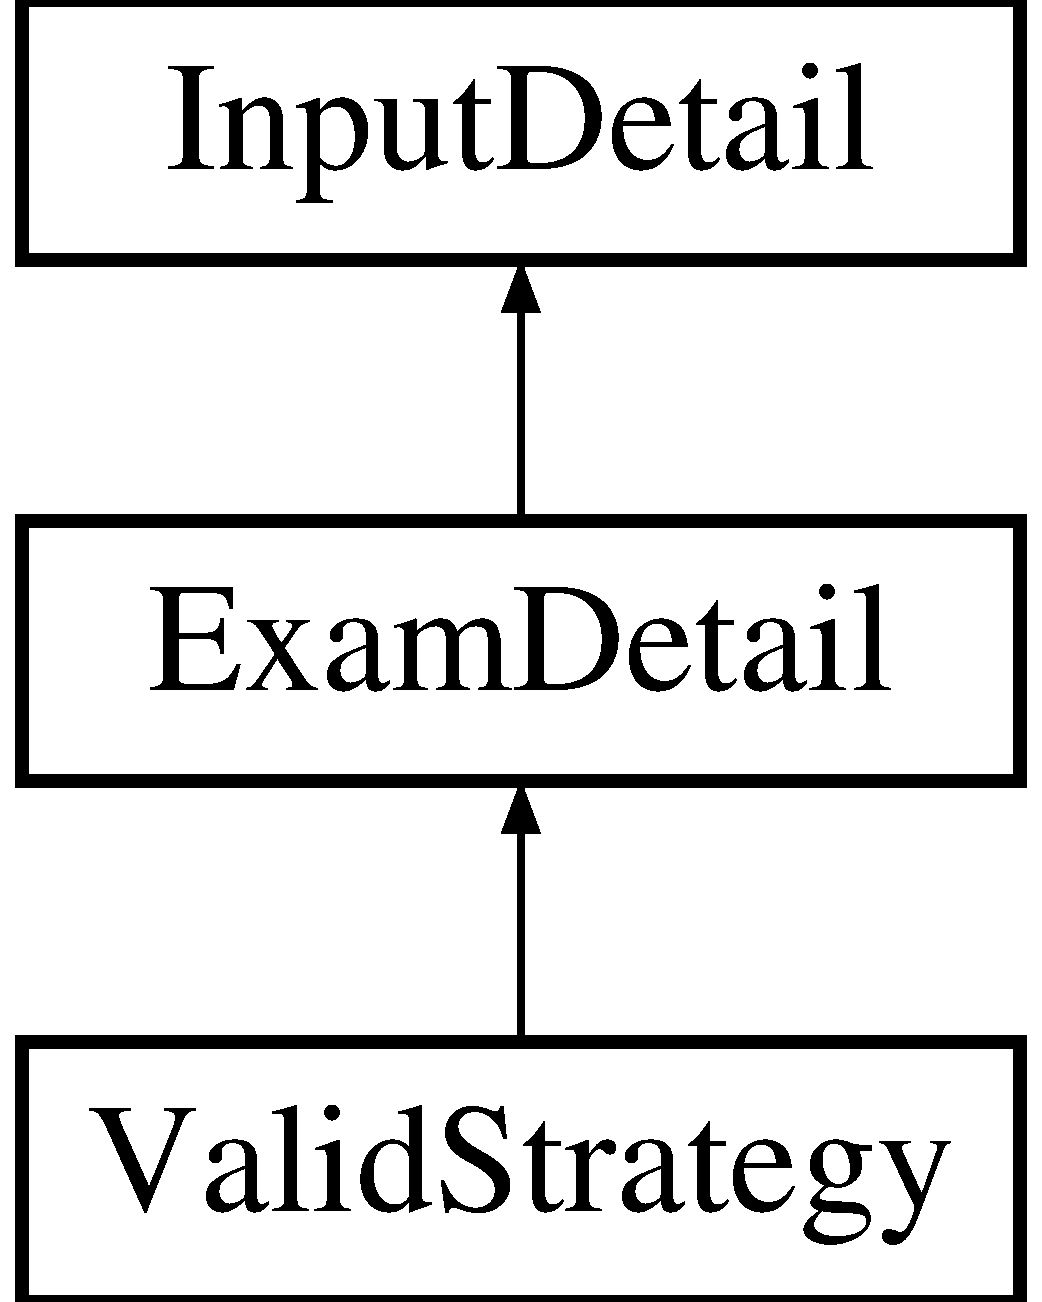
\includegraphics[height=2.000000cm]{classValidStrategy}
\end{center}
\end{figure}
\subsection*{Public Member Functions}
\begin{DoxyCompactItemize}
\item 
\hyperlink{classValidStrategy_ae168db88ebfa1eabdd7f241a631ffc27}{Valid\-Strategy} ()
\begin{DoxyCompactList}\small\item\em Constructor. \end{DoxyCompactList}\item 
void \hyperlink{classValidStrategy_ae8b17f98d81f8f70d974139086495dfa}{Read\-Strategy\-Detail} ()
\begin{DoxyCompactList}\small\item\em Reading strategy value from last page. \end{DoxyCompactList}\item 
void \hyperlink{classValidStrategy_a093620e19cef0865e6e38a26bb41b8bd}{Write\-Strategy\-Detail} ()
\begin{DoxyCompactList}\small\item\em Write strategy detail into D\-B. \end{DoxyCompactList}\item 
void \hyperlink{classValidStrategy_a234ca3ab5aa4684306148afa47b6860b}{Read\-Valid\-Strategy} ()
\begin{DoxyCompactList}\small\item\em Reading validation file for checking strategy is valid or not. \end{DoxyCompactList}\item 
void \hyperlink{classValidStrategy_ad89451a935f815b4c85b595135d70d94}{Valid\-Strategy\-Page} ()
\begin{DoxyCompactList}\small\item\em Valid\-Strategy.\-html page. \end{DoxyCompactList}\item 
\hyperlink{classValidStrategy_aec9e6ff1c9e9058a17f5488fe3e6cfec}{$\sim$\-Valid\-Strategy} ()
\begin{DoxyCompactList}\small\item\em Destructor. \end{DoxyCompactList}\end{DoxyCompactItemize}
\subsection*{Protected Attributes}
\begin{DoxyCompactItemize}
\item 
\hypertarget{classValidStrategy_aac23ca61c16d79b48603a7db96617003}{\hyperlink{classStrategy}{Strategy} {\bfseries valid\-Strategy}}\label{classValidStrategy_aac23ca61c16d79b48603a7db96617003}

\item 
\hypertarget{classValidStrategy_a0400bdc1d25df2a613d50ed02c537eb2}{S\-T\-R\-I\-N\-G\-\_\-\-V\-E\-C {\bfseries selected\-Strategy}}\label{classValidStrategy_a0400bdc1d25df2a613d50ed02c537eb2}

\item 
\hypertarget{classValidStrategy_ad34fa679672d7685af9678e6c579e800}{S\-T\-R\-I\-N\-G\-\_\-\-V\-E\-C {\bfseries total\-Seats}}\label{classValidStrategy_ad34fa679672d7685af9678e6c579e800}

\item 
\hypertarget{classValidStrategy_a7344a7cf32192fa494ed9dd6784c509e}{S\-T\-R\-I\-N\-G\-\_\-\-V\-E\-C {\bfseries total\-Group\-Seats}}\label{classValidStrategy_a7344a7cf32192fa494ed9dd6784c509e}

\item 
\hypertarget{classValidStrategy_a4d0e361e6ed28a83332bebf66ab018e2}{S\-T\-R\-I\-N\-G\-\_\-\-V\-E\-C {\bfseries total\-Students}}\label{classValidStrategy_a4d0e361e6ed28a83332bebf66ab018e2}

\item 
\hypertarget{classValidStrategy_a4d947570307ce9d87d35f699ee10cae6}{S\-T\-R\-I\-N\-G\-\_\-\-V\-E\-C {\bfseries total\-Group\-Students}}\label{classValidStrategy_a4d947570307ce9d87d35f699ee10cae6}

\item 
\hypertarget{classValidStrategy_a66d7ba02a423a08f4f0af7c714787e76}{S\-T\-R\-I\-N\-G\-\_\-\-V\-E\-C {\bfseries valid}}\label{classValidStrategy_a66d7ba02a423a08f4f0af7c714787e76}

\item 
\hypertarget{classValidStrategy_aa18f4ff7dd65ed5702148c192f8627a6}{bool {\bfseries add\-Room}}\label{classValidStrategy_aa18f4ff7dd65ed5702148c192f8627a6}

\end{DoxyCompactItemize}
\subsection*{Additional Inherited Members}


\subsection{Detailed Description}
include inpudetail.\-h 

Definition at line 25 of file validstrategy.\-h.



\subsection{Constructor \& Destructor Documentation}
\hypertarget{classValidStrategy_ae168db88ebfa1eabdd7f241a631ffc27}{\index{Valid\-Strategy@{Valid\-Strategy}!Valid\-Strategy@{Valid\-Strategy}}
\index{Valid\-Strategy@{Valid\-Strategy}!ValidStrategy@{Valid\-Strategy}}
\subsubsection[{Valid\-Strategy}]{\setlength{\rightskip}{0pt plus 5cm}Valid\-Strategy\-::\-Valid\-Strategy (
\begin{DoxyParamCaption}
{}
\end{DoxyParamCaption}
)}}\label{classValidStrategy_ae168db88ebfa1eabdd7f241a631ffc27}


Constructor. 

Constructor 

Definition at line 24 of file validstrategy.\-cc.

\hypertarget{classValidStrategy_aec9e6ff1c9e9058a17f5488fe3e6cfec}{\index{Valid\-Strategy@{Valid\-Strategy}!$\sim$\-Valid\-Strategy@{$\sim$\-Valid\-Strategy}}
\index{$\sim$\-Valid\-Strategy@{$\sim$\-Valid\-Strategy}!ValidStrategy@{Valid\-Strategy}}
\subsubsection[{$\sim$\-Valid\-Strategy}]{\setlength{\rightskip}{0pt plus 5cm}Valid\-Strategy\-::$\sim$\-Valid\-Strategy (
\begin{DoxyParamCaption}
{}
\end{DoxyParamCaption}
)}}\label{classValidStrategy_aec9e6ff1c9e9058a17f5488fe3e6cfec}


Destructor. 

desrtuctor 

Definition at line 271 of file validstrategy.\-cc.



\subsection{Member Function Documentation}
\hypertarget{classValidStrategy_ae8b17f98d81f8f70d974139086495dfa}{\index{Valid\-Strategy@{Valid\-Strategy}!Read\-Strategy\-Detail@{Read\-Strategy\-Detail}}
\index{Read\-Strategy\-Detail@{Read\-Strategy\-Detail}!ValidStrategy@{Valid\-Strategy}}
\subsubsection[{Read\-Strategy\-Detail}]{\setlength{\rightskip}{0pt plus 5cm}void Valid\-Strategy\-::\-Read\-Strategy\-Detail (
\begin{DoxyParamCaption}
{}
\end{DoxyParamCaption}
)}}\label{classValidStrategy_ae8b17f98d81f8f70d974139086495dfa}


Reading strategy value from last page. 

Read \hyperlink{classStrategy}{Strategy} Detail 

Definition at line 46 of file validstrategy.\-cc.

\hypertarget{classValidStrategy_a234ca3ab5aa4684306148afa47b6860b}{\index{Valid\-Strategy@{Valid\-Strategy}!Read\-Valid\-Strategy@{Read\-Valid\-Strategy}}
\index{Read\-Valid\-Strategy@{Read\-Valid\-Strategy}!ValidStrategy@{Valid\-Strategy}}
\subsubsection[{Read\-Valid\-Strategy}]{\setlength{\rightskip}{0pt plus 5cm}void Valid\-Strategy\-::\-Read\-Valid\-Strategy (
\begin{DoxyParamCaption}
{}
\end{DoxyParamCaption}
)}}\label{classValidStrategy_a234ca3ab5aa4684306148afa47b6860b}


Reading validation file for checking strategy is valid or not. 

Read Valid\-Strategy.\-out file 

Definition at line 131 of file validstrategy.\-cc.

\hypertarget{classValidStrategy_ad89451a935f815b4c85b595135d70d94}{\index{Valid\-Strategy@{Valid\-Strategy}!Valid\-Strategy\-Page@{Valid\-Strategy\-Page}}
\index{Valid\-Strategy\-Page@{Valid\-Strategy\-Page}!ValidStrategy@{Valid\-Strategy}}
\subsubsection[{Valid\-Strategy\-Page}]{\setlength{\rightskip}{0pt plus 5cm}void Valid\-Strategy\-::\-Valid\-Strategy\-Page (
\begin{DoxyParamCaption}
{}
\end{DoxyParamCaption}
)}}\label{classValidStrategy_ad89451a935f815b4c85b595135d70d94}


Valid\-Strategy.\-html page. 

\hyperlink{classValidStrategy}{Valid\-Strategy} Page 

Definition at line 185 of file validstrategy.\-cc.

\hypertarget{classValidStrategy_a093620e19cef0865e6e38a26bb41b8bd}{\index{Valid\-Strategy@{Valid\-Strategy}!Write\-Strategy\-Detail@{Write\-Strategy\-Detail}}
\index{Write\-Strategy\-Detail@{Write\-Strategy\-Detail}!ValidStrategy@{Valid\-Strategy}}
\subsubsection[{Write\-Strategy\-Detail}]{\setlength{\rightskip}{0pt plus 5cm}void Valid\-Strategy\-::\-Write\-Strategy\-Detail (
\begin{DoxyParamCaption}
{}
\end{DoxyParamCaption}
)}}\label{classValidStrategy_a093620e19cef0865e6e38a26bb41b8bd}


Write strategy detail into D\-B. 

Write \hyperlink{classStrategy}{Strategy} Detail 

Definition at line 80 of file validstrategy.\-cc.



The documentation for this class was generated from the following files\-:\begin{DoxyCompactItemize}
\item 
frontend/src/header/validstrategy.\-h\item 
frontend/src/validstrategy.\-cc\end{DoxyCompactItemize}

\chapter{File Documentation}
\hypertarget{adduser-main_8cpp}{\section{frontend/src/adduser-\/main.cpp File Reference}
\label{adduser-main_8cpp}\index{frontend/src/adduser-\/main.\-cpp@{frontend/src/adduser-\/main.\-cpp}}
}


Adding new user and setting its password.  


{\ttfamily \#include \char`\"{}header/login.\-h\char`\"{}}\\*
\subsection*{Functions}
\begin{DoxyCompactItemize}
\item 
\hypertarget{adduser-main_8cpp_a840291bc02cba5474a4cb46a9b9566fe}{int {\bfseries main} (void)}\label{adduser-main_8cpp_a840291bc02cba5474a4cb46a9b9566fe}

\end{DoxyCompactItemize}


\subsection{Detailed Description}
Adding new user and setting its password. \begin{DoxyVersion}{Version}
0.\-8 
\end{DoxyVersion}
\begin{DoxyDate}{Date}
Sunday 07 April 2013 01\-:15\-:32 I\-S\-T\par
Compiler g++
\end{DoxyDate}
\begin{DoxyAuthor}{Author}
Mandeep Kaur, \href{mailto:meghasimak@gmail.com}{\tt meghasimak@gmail.\-com} License G\-N\-U General Public License 
\end{DoxyAuthor}
\begin{DoxyCopyright}{Copyright}
Copyright (c) 2013, Great\-Developers \href{https://github.com/GreatDevelopers}{\tt https\-://github.\-com/\-Great\-Developers} 
\end{DoxyCopyright}


Definition in file \hyperlink{adduser-main_8cpp_source}{adduser-\/main.\-cpp}.


\hypertarget{arrangerollno_8cc}{\section{frontend/src/backend/arrangerollno.cc File Reference}
\label{arrangerollno_8cc}\index{frontend/src/backend/arrangerollno.\-cc@{frontend/src/backend/arrangerollno.\-cc}}
}


Function definition of \hyperlink{classArrangeRollNo}{Arrange\-Roll\-No} class.  


{\ttfamily \#include \char`\"{}header/arrangerollno.\-h\char`\"{}}\\*


\subsection{Detailed Description}
Function definition of \hyperlink{classArrangeRollNo}{Arrange\-Roll\-No} class. \begin{DoxyVersion}{Version}
0.\-7 
\end{DoxyVersion}
\begin{DoxyDate}{Date}
Sunday 31 March 2013 06\-:50\-:00 I\-S\-T\par
Compiler g++
\end{DoxyDate}
\begin{DoxyAuthor}{Author}
Mandeep Kaur, \href{mailto:meghasimak@gmail.com}{\tt meghasimak@gmail.\-com} License G\-N\-U General Public License 
\end{DoxyAuthor}
\begin{DoxyCopyright}{Copyright}
Copyright (c) 2013, Great\-Developers \href{https://github.com/GreatDevelopers}{\tt https\-://github.\-com/\-Great\-Developers} 
\end{DoxyCopyright}


Definition in file \hyperlink{arrangerollno_8cc_source}{arrangerollno.\-cc}.


\hypertarget{expandrollno_8cc}{\section{frontend/src/backend/expandrollno.cc \-File \-Reference}
\label{expandrollno_8cc}\index{frontend/src/backend/expandrollno.\-cc@{frontend/src/backend/expandrollno.\-cc}}
}


\-Function definition of \hyperlink{classExpandRollNo}{\-Expand\-Roll\-No} class defintion.  


{\ttfamily \#include \char`\"{}header/expandrollno.\-h\char`\"{}}\*


\subsection{\-Detailed \-Description}
\-Function definition of \hyperlink{classExpandRollNo}{\-Expand\-Roll\-No} class defintion. \begin{DoxyVersion}{\-Version}
0.\-7 
\end{DoxyVersion}
\begin{DoxyDate}{\-Date}
\-Sunday 31 \-March 2013 06\-:49\-:23 \-I\-S\-T\par
 \-Compiler g++
\end{DoxyDate}
\begin{DoxyAuthor}{\-Author}
\-Mandeep \-Kaur, \href{mailto:meghasimak@gmail.com}{\tt meghasimak@gmail.\-com} \-License \-G\-N\-U \-General \-Public \-License 
\end{DoxyAuthor}
\begin{DoxyCopyright}{\-Copyright}
\-Copyright (c) 2013, \-Great\-Developers \href{https://github.com/GreatDevelopers}{\tt https\-://github.\-com/\-Great\-Developers} 
\end{DoxyCopyright}


\-Definition in file \hyperlink{expandrollno_8cc_source}{expandrollno.\-cc}.


\hypertarget{arrangerollno_8h}{\section{frontend/src/backend/header/arrangerollno.h \-File \-Reference}
\label{d4/d7b/arrangerollno_8h}\index{frontend/src/backend/header/arrangerollno.\-h@{frontend/src/backend/header/arrangerollno.\-h}}
}


\hyperlink{classArrangeRollNo}{\-Arrange\-Roll\-No} class for arranging roll no, sorting, and removing roll nos that are not required for seating plan.  


{\ttfamily \#include \char`\"{}expandrollno.\-h\char`\"{}}\*
\subsection*{\-Classes}
\begin{DoxyCompactItemize}
\item 
class \hyperlink{classArrangeRollNo}{\-Arrange\-Roll\-No}
\begin{DoxyCompactList}\small\item\em \-Arrange roll no class for sorting, removing redundant roll nos and also excludeing roll nos that are not for seating plan. \end{DoxyCompactList}\end{DoxyCompactItemize}


\subsection{\-Detailed \-Description}
\hyperlink{classArrangeRollNo}{\-Arrange\-Roll\-No} class for arranging roll no, sorting, and removing roll nos that are not required for seating plan. \begin{DoxyVersion}{\-Version}
0.\-7 
\end{DoxyVersion}
\begin{DoxyDate}{\-Date}
\-Sunday 31 \-March 2013 06\-:33\-:39 \-I\-S\-T\par
 \-Compiler g++
\end{DoxyDate}
\begin{DoxyAuthor}{\-Author}
\-Mandeep \-Kaur, \href{mailto:meghasimak@gmail.com}{\tt meghasimak@gmail.\-com} \-License \-G\-N\-U \-General \-Public \-License 
\end{DoxyAuthor}
\begin{DoxyCopyright}{\-Copyright}
\-Copyright (c) 2013, \-Great\-Developers \href{https://github.com/GreatDevelopers}{\tt https\-://github.\-com/\-Great\-Developers} 
\end{DoxyCopyright}


\-Definition in file \hyperlink{arrangerollno_8h_source}{arrangerollno.\-h}.


\hypertarget{expandrollno_8h}{\section{src/backend/header/expandrollno.h File Reference}
\label{expandrollno_8h}\index{src/backend/header/expandrollno.\-h@{src/backend/header/expandrollno.\-h}}
}


\hyperlink{classExpandRollNo}{Expand\-Roll\-No} class declaration for expanding roll nos.  


{\ttfamily \#include \char`\"{}readinput.\-h\char`\"{}}\\*
\subsection*{Classes}
\begin{DoxyCompactItemize}
\item 
class \hyperlink{classExpandRollNo}{Expand\-Roll\-No}
\end{DoxyCompactItemize}


\subsection{Detailed Description}
\hyperlink{classExpandRollNo}{Expand\-Roll\-No} class declaration for expanding roll nos. \begin{DoxyVersion}{Version}
0.\-6 
\end{DoxyVersion}
\begin{DoxyDate}{Date}
Sunday 31 March 2013 05\-:45\-:55 I\-S\-T\par
 Compiler g++
\end{DoxyDate}
\begin{DoxyAuthor}{Author}
Mandeep Kaur, \href{mailto:meghasimak@gmail.com}{\tt meghasimak@gmail.\-com} License G\-N\-U General Public License 
\end{DoxyAuthor}
\begin{DoxyCopyright}{Copyright}
Copyright (c) 2013, Great\-Developers \href{https://github.com/GreatDevelopers}{\tt https\-://github.\-com/\-Great\-Developers} 
\end{DoxyCopyright}


Definition in file \hyperlink{expandrollno_8h_source}{expandrollno.\-h}.


\hypertarget{readinput_8h}{\section{frontend/src/backend/header/readinput.h \-File \-Reference}
\label{d3/d23/readinput_8h}\index{frontend/src/backend/header/readinput.\-h@{frontend/src/backend/header/readinput.\-h}}
}


\-Declaration of \hyperlink{classReadInput}{\-Read\-Input} class for reading input details from file.  


{\ttfamily \#include \char`\"{}header.\-h\char`\"{}}\*
\subsection*{\-Classes}
\begin{DoxyCompactItemize}
\item 
class \hyperlink{classReadInput}{\-Read\-Input}
\begin{DoxyCompactList}\small\item\em \-Class for reading input files ie reading roll no details, class detail, room detail, etc. \end{DoxyCompactList}\end{DoxyCompactItemize}


\subsection{\-Detailed \-Description}
\-Declaration of \hyperlink{classReadInput}{\-Read\-Input} class for reading input details from file. \begin{DoxyVersion}{\-Version}
0.\-7 
\end{DoxyVersion}
\begin{DoxyDate}{\-Date}
\-Sunday 31 \-March 2013 02\-:33\-:49 \-I\-S\-T\par
 \-Compiler g++
\end{DoxyDate}
\begin{DoxyAuthor}{\-Author}
\-Mandeep \-Kaur, \href{mailto:meghasimak@gmail.com}{\tt meghasimak@gmail.\-com} \-License \-G\-N\-U \-General \-Public \-License 
\end{DoxyAuthor}
\begin{DoxyCopyright}{\-Copyright}
\-Copyright (c) 2013, \-Great\-Developers \href{https://github.com/GreatDevelopers}{\tt https\-://github.\-com/\-Great\-Developers} 
\end{DoxyCopyright}


\-Definition in file \hyperlink{readinput_8h_source}{readinput.\-h}.


\hypertarget{seatplan_8h}{\section{frontend/src/backend/header/seatplan.h File Reference}
\label{seatplan_8h}\index{frontend/src/backend/header/seatplan.\-h@{frontend/src/backend/header/seatplan.\-h}}
}


Declaration of \hyperlink{classSeatPlan}{Seat\-Plan} class for generating seating plan.  


{\ttfamily \#include \char`\"{}readinput.\-h\char`\"{}}\\*
\subsection*{Classes}
\begin{DoxyCompactItemize}
\item 
class \hyperlink{classSeatPlan}{Seat\-Plan}
\begin{DoxyCompactList}\small\item\em \hyperlink{classSeatPlan}{Seat\-Plan} C\-Lass for generating seating plan. \end{DoxyCompactList}\end{DoxyCompactItemize}


\subsection{Detailed Description}
Declaration of \hyperlink{classSeatPlan}{Seat\-Plan} class for generating seating plan. \begin{DoxyVersion}{Version}
0.\-7 
\end{DoxyVersion}
\begin{DoxyDate}{Date}
Tuesday 02 April 2013 02\-:05\-:39 I\-S\-T\par
 Compiler g++
\end{DoxyDate}
\begin{DoxyAuthor}{Author}
Mandeep Kaur, \href{mailto:meghasimak@gmail.com}{\tt meghasimak@gmail.\-com} License G\-N\-U General Public License 
\end{DoxyAuthor}
\begin{DoxyCopyright}{Copyright}
Copyright (c) 2013, Great\-Developers \href{https://github.com/GreatDevelopers}{\tt https\-://github.\-com/\-Great\-Developers} 
\end{DoxyCopyright}


Definition in file \hyperlink{seatplan_8h_source}{seatplan.\-h}.


\hypertarget{main_8cpp}{\section{frontend/src/backend/main.cpp File Reference}
\label{main_8cpp}\index{frontend/src/backend/main.\-cpp@{frontend/src/backend/main.\-cpp}}
}


Main Method.  


{\ttfamily \#include \char`\"{}header/datesheet.\-h\char`\"{}}\\*
{\ttfamily \#include \char`\"{}header/strategy.\-h\char`\"{}}\\*
\subsection*{Functions}
\begin{DoxyCompactItemize}
\item 
\hypertarget{main_8cpp_a840291bc02cba5474a4cb46a9b9566fe}{int {\bfseries main} (void)}\label{main_8cpp_a840291bc02cba5474a4cb46a9b9566fe}

\end{DoxyCompactItemize}


\subsection{Detailed Description}
Main Method. \begin{DoxyVersion}{Version}
0.\-7 
\end{DoxyVersion}
\begin{DoxyDate}{Date}
Sunday 31 March 2013 08\-:13\-:40 I\-S\-T\par
 Compiler g++
\end{DoxyDate}
\begin{DoxyAuthor}{Author}
Mandeep Kaur, \href{mailto:meghasimak@gmail.com}{\tt meghasimak@gmail.\-com} License G\-N\-U General Public License 
\end{DoxyAuthor}
\begin{DoxyCopyright}{Copyright}
Copyright (c) 2013, Great\-Developers \href{https://github.com/GreatDevelopers}{\tt https\-://github.\-com/\-Great\-Developers} 
\end{DoxyCopyright}


Definition in file \hyperlink{main_8cpp_source}{main.\-cpp}.


\hypertarget{readinput_8cc}{\section{src/cpp/backend/readinput.cc File Reference}
\label{readinput_8cc}\index{src/cpp/backend/readinput.\-cc@{src/cpp/backend/readinput.\-cc}}
}


Function Definition of \hyperlink{classReadInput}{Read\-Input} Class.  


{\ttfamily \#include \char`\"{}header/readinput.\-h\char`\"{}}\\*


\subsection{Detailed Description}
Function Definition of \hyperlink{classReadInput}{Read\-Input} Class. \begin{DoxyVersion}{Version}
0.\-8 
\end{DoxyVersion}
\begin{DoxyDate}{Date}
Sunday 31 March 2013 06\-:48\-:51 I\-S\-T\par
 Compiler g++
\end{DoxyDate}
\begin{DoxyAuthor}{Author}
Mandeep Kaur, \href{mailto:meghasimak@gmail.com}{\tt meghasimak@gmail.\-com} License G\-N\-U General Public License 
\end{DoxyAuthor}
\begin{DoxyCopyright}{Copyright}
Copyright (c) 2013, Great\-Developers \href{https://github.com/GreatDevelopers}{\tt https\-://github.\-com/\-Great\-Developers} 
\end{DoxyCopyright}


Definition in file \hyperlink{readinput_8cc_source}{readinput.\-cc}.


\hypertarget{seatplan_8cc}{\section{frontend/src/backend/seatplan.cc File Reference}
\label{seatplan_8cc}\index{frontend/src/backend/seatplan.\-cc@{frontend/src/backend/seatplan.\-cc}}
}


Function definition of \hyperlink{classSeatPlan}{Seat\-Plan} Class.  


{\ttfamily \#include \char`\"{}header/seatplan.\-h\char`\"{}}\\*


\subsection{Detailed Description}
Function definition of \hyperlink{classSeatPlan}{Seat\-Plan} Class. \begin{DoxyVersion}{Version}
0.\-7 
\end{DoxyVersion}
\begin{DoxyDate}{Date}
Tuesday 02 April 2013 02\-:44\-:21 I\-S\-T\par
 Compiler g++
\end{DoxyDate}
\begin{DoxyAuthor}{Author}
Mandeep Kaur, \href{mailto:meghasimak@gmail.com}{\tt meghasimak@gmail.\-com} License G\-N\-U General Public License 
\end{DoxyAuthor}
\begin{DoxyCopyright}{Copyright}
Copyright (c) 2013, Great\-Developers \href{https://github.com/GreatDevelopers}{\tt https\-://github.\-com/\-Great\-Developers} 
\end{DoxyCopyright}


Definition in file \hyperlink{seatplan_8cc_source}{seatplan.\-cc}.


\hypertarget{class-main_8cpp}{\section{frontend/src/class-\/main.cpp File Reference}
\label{class-main_8cpp}\index{frontend/src/class-\/main.\-cpp@{frontend/src/class-\/main.\-cpp}}
}


main method  


{\ttfamily \#include \char`\"{}header/class.\-h\char`\"{}}\\*
\subsection*{Functions}
\begin{DoxyCompactItemize}
\item 
\hypertarget{class-main_8cpp_a840291bc02cba5474a4cb46a9b9566fe}{int {\bfseries main} (void)}\label{class-main_8cpp_a840291bc02cba5474a4cb46a9b9566fe}

\end{DoxyCompactItemize}


\subsection{Detailed Description}
main method \begin{DoxyVersion}{Version}
0.\-7 
\end{DoxyVersion}
\begin{DoxyDate}{Date}
Sunday 07 April 2013 09\-:00\-:37 I\-S\-T\par
Compiler g++
\end{DoxyDate}
\begin{DoxyAuthor}{Author}
Mandeep Kaur, \href{mailto:meghasimak@gmail.com}{\tt meghasimak@gmail.\-com} License G\-N\-U General Public License 
\end{DoxyAuthor}
\begin{DoxyCopyright}{Copyright}
Copyright (c) 2013, Great\-Developers \href{https://github.com/GreatDevelopers}{\tt https\-://github.\-com/\-Great\-Developers} 
\end{DoxyCopyright}


Definition in file \hyperlink{class-main_8cpp_source}{class-\/main.\-cpp}.


\hypertarget{class_8cc}{\section{frontend/src/class.cc \-File \-Reference}
\label{d6/df2/class_8cc}\index{frontend/src/class.\-cc@{frontend/src/class.\-cc}}
}


\hyperlink{classClassDetail}{\-Class\-Detail} function definition.  


{\ttfamily \#include \char`\"{}header/class.\-h\char`\"{}}\*


\subsection{\-Detailed \-Description}
\hyperlink{classClassDetail}{\-Class\-Detail} function definition. \begin{DoxyVersion}{\-Version}
0.\-7 
\end{DoxyVersion}
\begin{DoxyDate}{\-Date}
\-Sunday 07 \-April 2013 07\-:49\-:18 \-I\-S\-T\par
 \-Compiler g++
\end{DoxyDate}
\begin{DoxyAuthor}{\-Author}
\-Mandeep \-Kaur, \href{mailto:meghasimak@gmail.com}{\tt meghasimak@gmail.\-com} \-License \-G\-N\-U \-General \-Public \-License 
\end{DoxyAuthor}
\begin{DoxyCopyright}{\-Copyright}
\-Copyright (c) 2013, \-Great\-Developers \href{https://github.com/GreatDevelopers}{\tt https\-://github.\-com/\-Great\-Developers} 
\end{DoxyCopyright}


\-Definition in file \hyperlink{class_8cc_source}{class.\-cc}.


\hypertarget{confirm-main_8cpp}{\section{src/confirm-\/main.cpp File Reference}
\label{confirm-main_8cpp}\index{src/confirm-\/main.\-cpp@{src/confirm-\/main.\-cpp}}
}


Main method to call Confirm\-Page of \hyperlink{classLogin}{Login} class and creating confirm.\-html page.  


{\ttfamily \#include \char`\"{}header/login.\-h\char`\"{}}\\*
\subsection*{Functions}
\begin{DoxyCompactItemize}
\item 
\hypertarget{confirm-main_8cpp_a840291bc02cba5474a4cb46a9b9566fe}{int {\bfseries main} (void)}\label{confirm-main_8cpp_a840291bc02cba5474a4cb46a9b9566fe}

\end{DoxyCompactItemize}


\subsection{Detailed Description}
Main method to call Confirm\-Page of \hyperlink{classLogin}{Login} class and creating confirm.\-html page. \begin{DoxyVersion}{Version}
0.\-6 
\end{DoxyVersion}
\begin{DoxyDate}{Date}
Sunday 07 April 2013 07\-:40\-:31 I\-S\-T\par
 Compiler g++
\end{DoxyDate}
\begin{DoxyAuthor}{Author}
Mandeep Kaur, \href{mailto:meghasimak@gmail.com}{\tt meghasimak@gmail.\-com} License G\-N\-U General Public License 
\end{DoxyAuthor}
\begin{DoxyCopyright}{Copyright}
Copyright (c) 2013, Great\-Developers \href{https://github.com/GreatDevelopers}{\tt https\-://github.\-com/\-Great\-Developers} 
\end{DoxyCopyright}


Definition in file \hyperlink{confirm-main_8cpp_source}{confirm-\/main.\-cpp}.


\hypertarget{datesheet-main_8cpp}{\section{src/datesheet-\/main.cpp File Reference}
\label{datesheet-main_8cpp}\index{src/datesheet-\/main.\-cpp@{src/datesheet-\/main.\-cpp}}
}


main method  


{\ttfamily \#include \char`\"{}header/datesheet.\-h\char`\"{}}\\*
\subsection*{Functions}
\begin{DoxyCompactItemize}
\item 
\hypertarget{datesheet-main_8cpp_a840291bc02cba5474a4cb46a9b9566fe}{int {\bfseries main} (void)}\label{datesheet-main_8cpp_a840291bc02cba5474a4cb46a9b9566fe}

\end{DoxyCompactItemize}


\subsection{Detailed Description}
main method \begin{DoxyVersion}{Version}
0.\-6 
\end{DoxyVersion}
\begin{DoxyDate}{Date}
Sunday 07 April 2013 09\-:00\-:37 I\-S\-T\par
 Compiler g++
\end{DoxyDate}
\begin{DoxyAuthor}{Author}
Mandeep Kaur, \href{mailto:meghasimak@gmail.com}{\tt meghasimak@gmail.\-com} License G\-N\-U General Public License 
\end{DoxyAuthor}
\begin{DoxyCopyright}{Copyright}
Copyright (c) 2013, Great\-Developers \href{https://github.com/GreatDevelopers}{\tt https\-://github.\-com/\-Great\-Developers} 
\end{DoxyCopyright}


Definition in file \hyperlink{datesheet-main_8cpp_source}{datesheet-\/main.\-cpp}.


\hypertarget{exam-main_8cpp}{\section{frontend/src/exam-\/main.cpp \-File \-Reference}
\label{exam-main_8cpp}\index{frontend/src/exam-\/main.\-cpp@{frontend/src/exam-\/main.\-cpp}}
}


main method  


{\ttfamily \#include \char`\"{}header/exam.\-h\char`\"{}}\*
\subsection*{\-Functions}
\begin{DoxyCompactItemize}
\item 
\hypertarget{exam-main_8cpp_a840291bc02cba5474a4cb46a9b9566fe}{int {\bfseries main} (void)}\label{exam-main_8cpp_a840291bc02cba5474a4cb46a9b9566fe}

\end{DoxyCompactItemize}


\subsection{\-Detailed \-Description}
main method \begin{DoxyVersion}{\-Version}
0.\-7 
\end{DoxyVersion}
\begin{DoxyDate}{\-Date}
\-Sunday 07 \-April 2013 09\-:00\-:37 \-I\-S\-T\par
 \-Compiler g++
\end{DoxyDate}
\begin{DoxyAuthor}{\-Author}
\-Mandeep \-Kaur, \href{mailto:meghasimak@gmail.com}{\tt meghasimak@gmail.\-com} \-License \-G\-N\-U \-General \-Public \-License 
\end{DoxyAuthor}
\begin{DoxyCopyright}{\-Copyright}
\-Copyright (c) 2013, \-Great\-Developers \href{https://github.com/GreatDevelopers}{\tt https\-://github.\-com/\-Great\-Developers} 
\end{DoxyCopyright}


\-Definition in file \hyperlink{exam-main_8cpp_source}{exam-\/main.\-cpp}.


\hypertarget{exam_8cc}{\section{src/exam.cc File Reference}
\label{exam_8cc}\index{src/exam.\-cc@{src/exam.\-cc}}
}


\hyperlink{classExamDetail}{Exam\-Detail} Class func. definition.  


{\ttfamily \#include \char`\"{}header/exam.\-h\char`\"{}}\\*


\subsection{Detailed Description}
\hyperlink{classExamDetail}{Exam\-Detail} Class func. definition. \begin{DoxyVersion}{Version}
0.\-6 
\end{DoxyVersion}
\begin{DoxyDate}{Date}
Sunday 07 April 2013 08\-:04\-:21 I\-S\-T\par
 Compiler g++
\end{DoxyDate}
\begin{DoxyAuthor}{Author}
Mandeep Kaur, \href{mailto:meghasimak@gmail.com}{\tt meghasimak@gmail.\-com} License G\-N\-U General Public License 
\end{DoxyAuthor}
\begin{DoxyCopyright}{Copyright}
Copyright (c) 2013, Great\-Developers \href{https://github.com/GreatDevelopers}{\tt https\-://github.\-com/\-Great\-Developers} 
\end{DoxyCopyright}


Definition in file \hyperlink{exam_8cc_source}{exam.\-cc}.


\hypertarget{class_8h}{\section{frontend/src/header/class.h File Reference}
\label{class_8h}\index{frontend/src/header/class.\-h@{frontend/src/header/class.\-h}}
}


\hyperlink{classClassDetail}{Class\-Detail} Class declaration for displaying form for taking values from user. Input details like class/branch name, subject code and subject names.  


{\ttfamily \#include \char`\"{}project.\-h\char`\"{}}\\*
\subsection*{Classes}
\begin{DoxyCompactItemize}
\item 
class \hyperlink{classClassDetail}{Class\-Detail}
\begin{DoxyCompactList}\small\item\em For getting class details and reading project detail filled by user. \end{DoxyCompactList}\end{DoxyCompactItemize}


\subsection{Detailed Description}
\hyperlink{classClassDetail}{Class\-Detail} Class declaration for displaying form for taking values from user. Input details like class/branch name, subject code and subject names. \begin{DoxyVersion}{Version}
0.\-7 
\end{DoxyVersion}
\begin{DoxyDate}{Date}
Sunday 07 April 2013 07\-:45\-:59 I\-S\-T\par
 Compiler g++
\end{DoxyDate}
\begin{DoxyAuthor}{Author}
Mandeep Kaur, \href{mailto:meghasimak@gmail.com}{\tt meghasimak@gmail.\-com} License G\-N\-U General Public License 
\end{DoxyAuthor}
\begin{DoxyCopyright}{Copyright}
Copyright (c) 2013, Great\-Developers \href{https://github.com/GreatDevelopers}{\tt https\-://github.\-com/\-Great\-Developers} 
\end{DoxyCopyright}


Definition in file \hyperlink{class_8h_source}{class.\-h}.


\hypertarget{exam_8h}{\section{frontend/src/header/exam.h \-File \-Reference}
\label{exam_8h}\index{frontend/src/header/exam.\-h@{frontend/src/header/exam.\-h}}
}


\hyperlink{classExamDetail}{\-Exam\-Detail} class for exam detail.  


{\ttfamily \#include \char`\"{}inputdetail.\-h\char`\"{}}\*
\subsection*{\-Classes}
\begin{DoxyCompactItemize}
\item 
class \hyperlink{classExamDetail}{\-Exam\-Detail}
\begin{DoxyCompactList}\small\item\em \hyperlink{classExamDetail}{\-Exam\-Detail} class for getting exam from user. \end{DoxyCompactList}\end{DoxyCompactItemize}


\subsection{\-Detailed \-Description}
\hyperlink{classExamDetail}{\-Exam\-Detail} class for exam detail. \begin{DoxyVersion}{\-Version}
0.\-7 
\end{DoxyVersion}
\begin{DoxyDate}{\-Date}
\-Sunday 07 \-April 2013 08\-:01\-:53 \-I\-S\-T\par
 \-Compiler g++
\end{DoxyDate}
\begin{DoxyAuthor}{\-Author}
\-Mandeep \-Kaur, \href{mailto:meghasimak@gmail.com}{\tt meghasimak@gmail.\-com} \-License \-G\-N\-U \-General \-Public \-License 
\end{DoxyAuthor}
\begin{DoxyCopyright}{\-Copyright}
\-Copyright (c) 2013, \-Great\-Developers \href{https://github.com/GreatDevelopers}{\tt https\-://github.\-com/\-Great\-Developers} 
\end{DoxyCopyright}


\-Definition in file \hyperlink{exam_8h_source}{exam.\-h}.


\hypertarget{rollno_8h}{\section{frontend/src/header/rollno.h File Reference}
\label{rollno_8h}\index{frontend/src/header/rollno.\-h@{frontend/src/header/rollno.\-h}}
}


Roll\-No class declaration for taking roll no detail.  


{\ttfamily \#include \char`\"{}inputdetail.\-h\char`\"{}}\\*
\subsection*{Classes}
\begin{DoxyCompactItemize}
\item 
class \hyperlink{classRollNoDetail}{Roll\-No\-Detail}
\begin{DoxyCompactList}\small\item\em \hyperlink{classRollNoDetail}{Roll\-No\-Detail} class for taking roll no detail from user. \end{DoxyCompactList}\end{DoxyCompactItemize}


\subsection{Detailed Description}
Roll\-No class declaration for taking roll no detail. \begin{DoxyVersion}{Version}
0.\-8 
\end{DoxyVersion}
\begin{DoxyDate}{Date}
Sunday 07 April 2013 07\-:51\-:45 I\-S\-T\par
Compiler g++
\end{DoxyDate}
\begin{DoxyAuthor}{Author}
Mandeep Kaur, \href{mailto:meghasimak@gmail.com}{\tt meghasimak@gmail.\-com} License G\-N\-U General Public License 
\end{DoxyAuthor}
\begin{DoxyCopyright}{Copyright}
Copyright (c) 2013, Great\-Developers \href{https://github.com/GreatDevelopers}{\tt https\-://github.\-com/\-Great\-Developers} 
\end{DoxyCopyright}


Definition in file \hyperlink{rollno_8h_source}{rollno.\-h}.


\hypertarget{room_8h}{\section{frontend/src/header/room.h \-File \-Reference}
\label{room_8h}\index{frontend/src/header/room.\-h@{frontend/src/header/room.\-h}}
}


\hyperlink{classRoomDetail}{\-Room\-Detail} class.  


{\ttfamily \#include \char`\"{}inputdetail.\-h\char`\"{}}\*
{\ttfamily \#include \char`\"{}../backend/header/datesheet.\-h\char`\"{}}\*
\subsection*{\-Classes}
\begin{DoxyCompactItemize}
\item 
class \hyperlink{classRoomDetail}{\-Room\-Detail}
\end{DoxyCompactItemize}


\subsection{\-Detailed \-Description}
\hyperlink{classRoomDetail}{\-Room\-Detail} class. \begin{DoxyVersion}{\-Version}
0.\-7 
\end{DoxyVersion}
\begin{DoxyDate}{\-Date}
\-Sunday 07 \-April 2013 08\-:14\-:54 \-I\-S\-T\par
 \-Compiler g++
\end{DoxyDate}
\begin{DoxyAuthor}{\-Author}
\-Mandeep \-Kaur, \href{mailto:meghasimak@gmail.com}{\tt meghasimak@gmail.\-com} \-License \-G\-N\-U \-General \-Public \-License 
\end{DoxyAuthor}
\begin{DoxyCopyright}{\-Copyright}
\-Copyright (c) 2013, \-Great\-Developers \href{https://github.com/GreatDevelopers}{\tt https\-://github.\-com/\-Great\-Developers} 
\end{DoxyCopyright}


\-Definition in file \hyperlink{room_8h_source}{room.\-h}.


\hypertarget{sendmail-detail_8h}{\section{frontend/src/header/sendmail-\/detail.h File Reference}
\label{sendmail-detail_8h}\index{frontend/src/header/sendmail-\/detail.\-h@{frontend/src/header/sendmail-\/detail.\-h}}
}


S\-M\-T\-P swttings detail.  


{\ttfamily \#include \char`\"{}constant.\-h\char`\"{}}\\*
\subsection*{Variables}
\begin{DoxyCompactItemize}
\item 
\hypertarget{sendmail-detail_8h_a6a17dd6df02d3a5118873bc84ce9801d}{const char {\bfseries S\-E\-N\-D\-E\-R\-\_\-\-E\-M\-A\-I\-L\-I\-D} \mbox{[}F\-I\-L\-E\-\_\-\-S\-I\-Z\-E\mbox{]} = \char`\"{}baithnekaplan@gmail.\-com\char`\"{}}\label{sendmail-detail_8h_a6a17dd6df02d3a5118873bc84ce9801d}

\item 
\hypertarget{sendmail-detail_8h_a5a43d9760874d06771eec35419dad507}{const char {\bfseries S\-E\-R\-V\-E\-R\-\_\-\-M\-A\-I\-L} \mbox{[}F\-I\-L\-E\-\_\-\-S\-I\-Z\-E\mbox{]} = \char`\"{}202.\-164.\-53.\-122\char`\"{}}\label{sendmail-detail_8h_a5a43d9760874d06771eec35419dad507}

\item 
\hypertarget{sendmail-detail_8h_af0dde2cd6a9fa974836b177b410e97fe}{const char {\bfseries U\-S\-E\-R\-N\-A\-M\-E} \mbox{[}F\-I\-L\-E\-\_\-\-S\-I\-Z\-E\mbox{]} = \char`\"{}/$\sim$mandeep\char`\"{}}\label{sendmail-detail_8h_af0dde2cd6a9fa974836b177b410e97fe}

\end{DoxyCompactItemize}


\subsection{Detailed Description}
S\-M\-T\-P swttings detail. \begin{DoxyVersion}{Version}
0.\-8 
\end{DoxyVersion}
\begin{DoxyDate}{Date}
Saturday 06 April 2013 10\-:46\-:54 I\-S\-T\par
Compiler g++
\end{DoxyDate}
\begin{DoxyAuthor}{Author}
Mandeep Kaur, \href{mailto:meghasimak@gmail.com}{\tt meghasimak@gmail.\-com} License G\-N\-U General Public License 
\end{DoxyAuthor}
\begin{DoxyCopyright}{Copyright}
Copyright (c) 2013, Great\-Developers \href{https://github.com/GreatDevelopers}{\tt https\-://github.\-com/\-Great\-Developers} 
\end{DoxyCopyright}


Definition in file \hyperlink{sendmail-detail_8h_source}{sendmail-\/detail.\-h}.


\hypertarget{sendmail_8h}{\section{frontend/src/header/sendmail.h File Reference}
\label{sendmail_8h}\index{frontend/src/header/sendmail.\-h@{frontend/src/header/sendmail.\-h}}
}


Declaration of \hyperlink{classSendMail}{Send\-Mail} Class usinf jw\-S\-M\-T\-P library.  


{\ttfamily \#include $<$iostream$>$}\\*
{\ttfamily \#include \char`\"{}jwsmtp/jwsmtp.\-h\char`\"{}}\\*
{\ttfamily \#include \char`\"{}sendmail-\/detail.\-h\char`\"{}}\\*
\subsection*{Classes}
\begin{DoxyCompactItemize}
\item 
class \hyperlink{classSendMail}{Send\-Mail}
\begin{DoxyCompactList}\small\item\em Class for sending mail to user for registeration and for changing password. \end{DoxyCompactList}\end{DoxyCompactItemize}


\subsection{Detailed Description}
Declaration of \hyperlink{classSendMail}{Send\-Mail} Class usinf jw\-S\-M\-T\-P library. \begin{DoxyVersion}{Version}
0.\-8 
\end{DoxyVersion}
\begin{DoxyDate}{Date}
Saturday 06 April 2013 07\-:46\-:27 I\-S\-T\par
Compiler g++
\end{DoxyDate}
\begin{DoxyAuthor}{Author}
Mandeep Kaur, \href{mailto:meghasimak@gmail.com}{\tt meghasimak@gmail.\-com} License G\-N\-U General Public License 
\end{DoxyAuthor}
\begin{DoxyCopyright}{Copyright}
Copyright (c) 2013, Great\-Developers \href{https://github.com/GreatDevelopers}{\tt https\-://github.\-com/\-Great\-Developers} 
\end{DoxyCopyright}


Definition in file \hyperlink{sendmail_8h_source}{sendmail.\-h}.


\hypertarget{javascript_8cc}{\section{src/javascript.cc File Reference}
\label{javascript_8cc}\index{src/javascript.\-cc@{src/javascript.\-cc}}
}


function definition of javascript class  


{\ttfamily \#include \char`\"{}header/javascript.\-h\char`\"{}}\\*


\subsection{Detailed Description}
function definition of javascript class \begin{DoxyVersion}{Version}
0.\-6 
\end{DoxyVersion}
\begin{DoxyDate}{Date}
Thursday 04 April 2013 09\-:15\-:01 I\-S\-T\par
 Compiler g++
\end{DoxyDate}
\begin{DoxyAuthor}{Author}
Mandeep Kaur, \href{mailto:meghasimak@gmail.com}{\tt meghasimak@gmail.\-com} License G\-N\-U General Public License 
\end{DoxyAuthor}
\begin{DoxyCopyright}{Copyright}
Copyright (c) 2013, Great\-Developers \href{https://github.com/GreatDevelopers}{\tt https\-://github.\-com/\-Great\-Developers} 
\end{DoxyCopyright}


Definition in file \hyperlink{javascript_8cc_source}{javascript.\-cc}.


\hypertarget{login-main_8cpp}{\section{frontend/src/login-\/main.cpp \-File \-Reference}
\label{d5/d3b/login-main_8cpp}\index{frontend/src/login-\/main.\-cpp@{frontend/src/login-\/main.\-cpp}}
}


\-Main \-Function for create login.\-html page.  


{\ttfamily \#include \char`\"{}header/login.\-h\char`\"{}}\*
\subsection*{\-Functions}
\begin{DoxyCompactItemize}
\item 
\hypertarget{login-main_8cpp_a840291bc02cba5474a4cb46a9b9566fe}{int {\bfseries main} (void)}\label{d5/d3b/login-main_8cpp_a840291bc02cba5474a4cb46a9b9566fe}

\end{DoxyCompactItemize}


\subsection{\-Detailed \-Description}
\-Main \-Function for create login.\-html page. \begin{DoxyVersion}{\-Version}
0.\-7 
\end{DoxyVersion}
\begin{DoxyDate}{\-Date}
\-Friday 05 \-April 2013 07\-:30\-:10 \-I\-S\-T\par
 \-Compiler g++
\end{DoxyDate}
\begin{DoxyAuthor}{\-Author}
\-Mandeep \-Kaur, \href{mailto:meghasimak@gmail.com}{\tt meghasimak@gmail.\-com} \-License \-G\-N\-U \-General \-Public \-License 
\end{DoxyAuthor}
\begin{DoxyCopyright}{\-Copyright}
\-Copyright (c) 2013, \-Great\-Developers \href{https://github.com/GreatDevelopers}{\tt https\-://github.\-com/\-Great\-Developers} 
\end{DoxyCopyright}


\-Definition in file \hyperlink{login-main_8cpp_source}{login-\/main.\-cpp}.


\hypertarget{logout-main_8cpp}{\section{frontend/src/logout-\/main.cpp \-File \-Reference}
\label{logout-main_8cpp}\index{frontend/src/logout-\/main.\-cpp@{frontend/src/logout-\/main.\-cpp}}
}


\-Log out user account.  


{\ttfamily \#include \char`\"{}header/login.\-h\char`\"{}}\*
\subsection*{\-Functions}
\begin{DoxyCompactItemize}
\item 
\hypertarget{logout-main_8cpp_a840291bc02cba5474a4cb46a9b9566fe}{int {\bfseries main} (void)}\label{logout-main_8cpp_a840291bc02cba5474a4cb46a9b9566fe}

\end{DoxyCompactItemize}


\subsection{\-Detailed \-Description}
\-Log out user account. \begin{DoxyVersion}{\-Version}
0.\-7 
\end{DoxyVersion}
\begin{DoxyDate}{\-Date}
\-Sunday 07 \-April 2013 04\-:29\-:47 \-I\-S\-T\par
 \-Compiler g++
\end{DoxyDate}
\begin{DoxyAuthor}{\-Author}
\-Mandeep \-Kaur, \href{mailto:meghasimak@gmail.com}{\tt meghasimak@gmail.\-com} \-License \-G\-N\-U \-General \-Public \-License 
\end{DoxyAuthor}
\begin{DoxyCopyright}{\-Copyright}
\-Copyright (c) 2013, \-Great\-Developers \href{https://github.com/GreatDevelopers}{\tt https\-://github.\-com/\-Great\-Developers} 
\end{DoxyCopyright}


\-Definition in file \hyperlink{logout-main_8cpp_source}{logout-\/main.\-cpp}.


\hypertarget{register-main_8cpp}{\section{frontend/src/register-\/main.cpp File Reference}
\label{register-main_8cpp}\index{frontend/src/register-\/main.\-cpp@{frontend/src/register-\/main.\-cpp}}
}


Main method for register.\-html.  


{\ttfamily \#include \char`\"{}header/login.\-h\char`\"{}}\\*
\subsection*{Functions}
\begin{DoxyCompactItemize}
\item 
int \hyperlink{register-main_8cpp_a840291bc02cba5474a4cb46a9b9566fe}{main} (void)
\end{DoxyCompactItemize}


\subsection{Detailed Description}
Main method for register.\-html. \begin{DoxyVersion}{Version}
0.\-7 
\end{DoxyVersion}
\begin{DoxyDate}{Date}
Friday 05 April 2013 10\-:56\-:56 I\-S\-T\par
 Compiler g++
\end{DoxyDate}
\begin{DoxyAuthor}{Author}
Mandeep Kaur, \href{mailto:meghasimak@gmail.com}{\tt meghasimak@gmail.\-com} License G\-N\-U General Public License 
\end{DoxyAuthor}
\begin{DoxyCopyright}{Copyright}
Copyright (c) 2013, Great\-Developers \href{https://github.com/GreatDevelopers}{\tt https\-://github.\-com/\-Great\-Developers} 
\end{DoxyCopyright}


Definition in file \hyperlink{register-main_8cpp_source}{register-\/main.\-cpp}.



\subsection{Function Documentation}
\hypertarget{register-main_8cpp_a840291bc02cba5474a4cb46a9b9566fe}{\index{register-\/main.\-cpp@{register-\/main.\-cpp}!main@{main}}
\index{main@{main}!register-main.cpp@{register-\/main.\-cpp}}
\subsubsection[{main}]{\setlength{\rightskip}{0pt plus 5cm}int main (
\begin{DoxyParamCaption}
\item[{void}]{}
\end{DoxyParamCaption}
)}}\label{register-main_8cpp_a840291bc02cba5474a4cb46a9b9566fe}
Include login.\-h Main method for creating register.\-html page using functions of \hyperlink{classLogin}{Login} class 

Definition at line 26 of file register-\/main.\-cpp.


\hypertarget{report-main_8cpp}{\section{frontend/src/report-\/main.cpp File Reference}
\label{report-main_8cpp}\index{frontend/src/report-\/main.\-cpp@{frontend/src/report-\/main.\-cpp}}
}


main method  


{\ttfamily \#include \char`\"{}header/report.\-h\char`\"{}}\\*
\subsection*{Functions}
\begin{DoxyCompactItemize}
\item 
\hypertarget{report-main_8cpp_a840291bc02cba5474a4cb46a9b9566fe}{int {\bfseries main} (void)}\label{report-main_8cpp_a840291bc02cba5474a4cb46a9b9566fe}

\end{DoxyCompactItemize}


\subsection{Detailed Description}
main method \begin{DoxyVersion}{Version}
0.\-7 
\end{DoxyVersion}
\begin{DoxyDate}{Date}
Sunday 07 April 2013 09\-:00\-:37 I\-S\-T\par
Compiler g++
\end{DoxyDate}
\begin{DoxyAuthor}{Author}
Mandeep Kaur, \href{mailto:meghasimak@gmail.com}{\tt meghasimak@gmail.\-com} License G\-N\-U General Public License 
\end{DoxyAuthor}
\begin{DoxyCopyright}{Copyright}
Copyright (c) 2013, Great\-Developers \href{https://github.com/GreatDevelopers}{\tt https\-://github.\-com/\-Great\-Developers} 
\end{DoxyCopyright}


Definition in file \hyperlink{report-main_8cpp_source}{report-\/main.\-cpp}.


\hypertarget{rollno-main_8cpp}{\section{frontend/src/rollno-\/main.cpp \-File \-Reference}
\label{rollno-main_8cpp}\index{frontend/src/rollno-\/main.\-cpp@{frontend/src/rollno-\/main.\-cpp}}
}


main method  


{\ttfamily \#include \char`\"{}header/rollno.\-h\char`\"{}}\*
\subsection*{\-Functions}
\begin{DoxyCompactItemize}
\item 
\hypertarget{rollno-main_8cpp_a840291bc02cba5474a4cb46a9b9566fe}{int {\bfseries main} (void)}\label{rollno-main_8cpp_a840291bc02cba5474a4cb46a9b9566fe}

\end{DoxyCompactItemize}


\subsection{\-Detailed \-Description}
main method \begin{DoxyVersion}{\-Version}
0.\-7 
\end{DoxyVersion}
\begin{DoxyDate}{\-Date}
\-Sunday 07 \-April 2013 09\-:00\-:37 \-I\-S\-T\par
 \-Compiler g++
\end{DoxyDate}
\begin{DoxyAuthor}{\-Author}
\-Mandeep \-Kaur, \href{mailto:meghasimak@gmail.com}{\tt meghasimak@gmail.\-com} \-License \-G\-N\-U \-General \-Public \-License 
\end{DoxyAuthor}
\begin{DoxyCopyright}{\-Copyright}
\-Copyright (c) 2013, \-Great\-Developers \href{https://github.com/GreatDevelopers}{\tt https\-://github.\-com/\-Great\-Developers} 
\end{DoxyCopyright}


\-Definition in file \hyperlink{rollno-main_8cpp_source}{rollno-\/main.\-cpp}.


\hypertarget{rollno_8cc}{\section{frontend/src/rollno.cc File Reference}
\label{rollno_8cc}\index{frontend/src/rollno.\-cc@{frontend/src/rollno.\-cc}}
}


Roll\-No detail Class definition.  


{\ttfamily \#include \char`\"{}header/rollno.\-h\char`\"{}}\\*


\subsection{Detailed Description}
Roll\-No detail Class definition. \begin{DoxyVersion}{Version}
0.\-8 
\end{DoxyVersion}
\begin{DoxyDate}{Date}
Sunday 07 April 2013 07\-:53\-:57 I\-S\-T\par
Compiler g++
\end{DoxyDate}
\begin{DoxyAuthor}{Author}
Mandeep Kaur, \href{mailto:meghasimak@gmail.com}{\tt meghasimak@gmail.\-com} License G\-N\-U General Public License 
\end{DoxyAuthor}
\begin{DoxyCopyright}{Copyright}
Copyright (c) 2013, Great\-Developers \href{https://github.com/GreatDevelopers}{\tt https\-://github.\-com/\-Great\-Developers} 
\end{DoxyCopyright}


Definition in file \hyperlink{rollno_8cc_source}{rollno.\-cc}.


\hypertarget{room-main_8cpp}{\section{src/room-\/main.cpp File Reference}
\label{room-main_8cpp}\index{src/room-\/main.\-cpp@{src/room-\/main.\-cpp}}
}


main method  


{\ttfamily \#include \char`\"{}header/room.\-h\char`\"{}}\\*
\subsection*{Functions}
\begin{DoxyCompactItemize}
\item 
\hypertarget{room-main_8cpp_a840291bc02cba5474a4cb46a9b9566fe}{int {\bfseries main} (void)}\label{room-main_8cpp_a840291bc02cba5474a4cb46a9b9566fe}

\end{DoxyCompactItemize}


\subsection{Detailed Description}
main method \begin{DoxyVersion}{Version}
0.\-6 
\end{DoxyVersion}
\begin{DoxyDate}{Date}
Sunday 07 April 2013 09\-:00\-:37 I\-S\-T\par
 Compiler g++
\end{DoxyDate}
\begin{DoxyAuthor}{Author}
Mandeep Kaur, \href{mailto:meghasimak@gmail.com}{\tt meghasimak@gmail.\-com} License G\-N\-U General Public License 
\end{DoxyAuthor}
\begin{DoxyCopyright}{Copyright}
Copyright (c) 2013, Great\-Developers \href{https://github.com/GreatDevelopers}{\tt https\-://github.\-com/\-Great\-Developers} 
\end{DoxyCopyright}


Definition in file \hyperlink{room-main_8cpp_source}{room-\/main.\-cpp}.


\hypertarget{room_8cc}{\section{frontend/src/room.cc File Reference}
\label{room_8cc}\index{frontend/src/room.\-cc@{frontend/src/room.\-cc}}
}


\hyperlink{classRoomDetail}{Room\-Detail} class definition.  


{\ttfamily \#include \char`\"{}header/room.\-h\char`\"{}}\\*


\subsection{Detailed Description}
\hyperlink{classRoomDetail}{Room\-Detail} class definition. \begin{DoxyVersion}{Version}
0.\-7 
\end{DoxyVersion}
\begin{DoxyDate}{Date}
Sunday 07 April 2013 08\-:17\-:36 I\-S\-T\par
 Compiler g++
\end{DoxyDate}
\begin{DoxyAuthor}{Author}
Mandeep Kaur, \href{mailto:meghasimak@gmail.com}{\tt meghasimak@gmail.\-com} License G\-N\-U General Public License 
\end{DoxyAuthor}
\begin{DoxyCopyright}{Copyright}
Copyright (c) 2013, Great\-Developers \href{https://github.com/GreatDevelopers}{\tt https\-://github.\-com/\-Great\-Developers} 
\end{DoxyCopyright}


Definition in file \hyperlink{room_8cc_source}{room.\-cc}.


\hypertarget{sendmail_8cc}{\section{frontend/src/sendmail.cc \-File \-Reference}
\label{sendmail_8cc}\index{frontend/src/sendmail.\-cc@{frontend/src/sendmail.\-cc}}
}


\-Function \-Definitons of \hyperlink{classSendMail}{\-Send\-Mail} \-Class.  


{\ttfamily \#include \char`\"{}header/sendmail.\-h\char`\"{}}\*


\subsection{\-Detailed \-Description}
\-Function \-Definitons of \hyperlink{classSendMail}{\-Send\-Mail} \-Class. \begin{DoxyVersion}{\-Version}
0.\-7 
\end{DoxyVersion}
\begin{DoxyDate}{\-Date}
\-Saturday 06 \-April 2013 07\-:58\-:56 \-I\-S\-T\par
 \-Compiler g++
\end{DoxyDate}
\begin{DoxyAuthor}{\-Author}
\-Mandeep \-Kaur, \href{mailto:meghasimak@gmail.com}{\tt meghasimak@gmail.\-com} \-License \-G\-N\-U \-General \-Public \-License 
\end{DoxyAuthor}
\begin{DoxyCopyright}{\-Copyright}
\-Copyright (c) 2013, \-Great\-Developers \href{https://github.com/GreatDevelopers}{\tt https\-://github.\-com/\-Great\-Developers} 
\end{DoxyCopyright}


\-Definition in file \hyperlink{sendmail_8cc_source}{sendmail.\-cc}.


\hypertarget{strategy-main_8cpp}{\section{src/strategy-\/main.cpp File Reference}
\label{strategy-main_8cpp}\index{src/strategy-\/main.\-cpp@{src/strategy-\/main.\-cpp}}
}


main method  


{\ttfamily \#include \char`\"{}header/strategy.\-h\char`\"{}}\\*
\subsection*{Functions}
\begin{DoxyCompactItemize}
\item 
\hypertarget{strategy-main_8cpp_a840291bc02cba5474a4cb46a9b9566fe}{int {\bfseries main} (void)}\label{strategy-main_8cpp_a840291bc02cba5474a4cb46a9b9566fe}

\end{DoxyCompactItemize}


\subsection{Detailed Description}
main method \begin{DoxyVersion}{Version}
0.\-6 
\end{DoxyVersion}
\begin{DoxyDate}{Date}
Sunday 07 April 2013 09\-:00\-:37 I\-S\-T\par
 Compiler g++
\end{DoxyDate}
\begin{DoxyAuthor}{Author}
Mandeep Kaur, \href{mailto:meghasimak@gmail.com}{\tt meghasimak@gmail.\-com} License G\-N\-U General Public License 
\end{DoxyAuthor}
\begin{DoxyCopyright}{Copyright}
Copyright (c) 2013, Great\-Developers \href{https://github.com/GreatDevelopers}{\tt https\-://github.\-com/\-Great\-Developers} 
\end{DoxyCopyright}


Definition in file \hyperlink{strategy-main_8cpp_source}{strategy-\/main.\-cpp}.


\hypertarget{validstrategy-main_8cpp}{\section{frontend/src/validstrategy-\/main.cpp \-File \-Reference}
\label{d9/dce/validstrategy-main_8cpp}\index{frontend/src/validstrategy-\/main.\-cpp@{frontend/src/validstrategy-\/main.\-cpp}}
}


main method  


{\ttfamily \#include \char`\"{}header/validstrategy.\-h\char`\"{}}\*
\subsection*{\-Functions}
\begin{DoxyCompactItemize}
\item 
\hypertarget{validstrategy-main_8cpp_a840291bc02cba5474a4cb46a9b9566fe}{int {\bfseries main} (void)}\label{d9/dce/validstrategy-main_8cpp_a840291bc02cba5474a4cb46a9b9566fe}

\end{DoxyCompactItemize}


\subsection{\-Detailed \-Description}
main method \begin{DoxyVersion}{\-Version}
0.\-7 
\end{DoxyVersion}
\begin{DoxyDate}{\-Date}
\-Sunday 07 \-April 2013 09\-:00\-:37 \-I\-S\-T\par
 \-Compiler g++
\end{DoxyDate}
\begin{DoxyAuthor}{\-Author}
\-Mandeep \-Kaur, \href{mailto:meghasimak@gmail.com}{\tt meghasimak@gmail.\-com} \-License \-G\-N\-U \-General \-Public \-License 
\end{DoxyAuthor}
\begin{DoxyCopyright}{\-Copyright}
\-Copyright (c) 2013, \-Great\-Developers \href{https://github.com/GreatDevelopers}{\tt https\-://github.\-com/\-Great\-Developers} 
\end{DoxyCopyright}


\-Definition in file \hyperlink{validstrategy-main_8cpp_source}{validstrategy-\/main.\-cpp}.


\addcontentsline{toc}{part}{Index}
\printindex
\end{document}
